%\documentclass[a4paper,12pt,twoside]{book}
\documentclass[listof=nochaptergap,12pt,times,authoryear]{report}
\usepackage{mathptmx}%This package supersedes times and mathptm
\usepackage[a4paper,right=2.54cm,left=2.54cm,top=2.54cm,bottom=2.54cm]{geometry}
\usepackage{array}
\usepackage{listings}
\usepackage{pdflscape}
\usepackage{longtable}
\usepackage{enumitem}
\usepackage{newclude}
\usepackage[export]{adjustbox}
\newcolumntype{C}[1]{>{\centering\arraybackslash}p{#1}}
\newcolumntype{N}{@{}m{0pt}@{}}
\newcommand\fillin[1][3cm]{\makebox[#1]{\dotfill}}

%%Paquete para ocultar indices de tabla de contenidos
%% Numeración continua en figuras y tablas
\setcounter{equation}{0}
\usepackage{chngcntr}
\counterwithout{figure}{chapter}
\counterwithout{table}{chapter}
\counterwithout{equation}{chapter}
\renewcommand{\thefigure}{\arabic{figure}}
\renewcommand{\thetable}{\arabic{table}}
\renewcommand{\theequation}{\arabic{equation}}

% Parche para eliminar espacios por capítulos en lista de figuras y tablas
\usepackage{etoolbox}% http://ctan.org/pkg/etoolbox
\makeatletter
% \patchcmd{<cmd>}{<search>}{<replace>}{<succes>}{<failure>}
\patchcmd{\@chapter}{\addtocontents{lof}{\protect\addvspace{10\p@}}}{}{}{}% LoF
\patchcmd{\@chapter}{\addtocontents{lot}{\protect\addvspace{10\p@}}}{}{}{}% LoT
\makeatother


%%%%paquete para usar citas de diferentes formatos
%%%%%%%%%%%%%%%%%%%%%%%%%%%%%%%%%
%%add al indice
%\usepackage[nottoc,numbib]{tocbibind}
%\usepackage[authoryear,round]{natbib}
\usepackage[T1]{fontenc}
\usepackage[utf8]{inputenc}
\usepackage{csquotes}
\usepackage[spanish,es-lcroman]{babel}
\decimalpoint
%% Citas y bibliografía formato APA
\usepackage[backend=biber,style=apa,natbib=true]{biblatex}
%\DeclareLanguageMapping{australian}{australian-apa}
\DeclareLanguageMapping{spanish}{spanish-apa}
\addbibresource{biblio/references.bib}

%% Formato DOI
\DeclareFieldFormat{doi}{%
	doi\addcolon\space
	\ifhyperref
	{\lowercase{\href{https://doi.org/#1}{\nolinkurl{#1}}}}
	{\lowercase{\nolinkurl{#1}}}}

%% Formato de URL en referencias
\DeclareFieldFormat{url}{{Recuperado de}\space\url{#1}}

%% Convertir comando cita por textcite para que tenga formato APA
\let\cite\textcite

%% Para que texto de figuras y tablas tenga formato APA.
%% Caption se carga aqui con sus opciones (margin/font/labelfont) en una sola
%% invocacion, para evitar "Option clash" si se intentara recargar mas abajo.
\usepackage{multirow,booktabs,setspace}
\usepackage[margin=10pt,font=small,labelfont=bf]{caption}
\DeclareCaptionLabelSeparator*{spaced}{\\[2ex]}
\captionsetup[table]{labelfont=normalfont,textfont=it,format=plain,justification=justified,singlelinecheck=false,labelsep=newline,skip=2pt}
\captionsetup[figure]{labelsep=period,labelfont={it,bf},justification=justified,singlelinecheck=false,font=doublespacing}
\captionsetup[subfigure]{justification=centering}

%%%Editar formato y tamaño de capítulos y secciones
\usepackage{titlesec}
\titleformat{\chapter}
{\centering\normalfont\large\bfseries}{Capítulo \thechapter:}{1em}{}
\titlespacing*{\chapter}{0pt}{-4ex}{1ex}

\titleformat{\section}
{\normalfont\large\bfseries}{\thesection}{1em}{}
\titlespacing*{\section}{0pt}{0pt}{0pt}

\titleformat{\subsection}
{\normalfont\large\bfseries}{\thesubsection}{1em}{}
\titlespacing*{\subsection}{0pt}{0pt}{0pt}

%\usepackage{biblatex}
%paquete para hiperlinks entre citas e imagenes
%%%%%%%%%%%%%%%%%%%%%%%%%%%%%%%%%
\usepackage[colorlinks=true,
citecolor=black,
urlcolor=black,
bookmarks=true,
linkcolor=black,
pdftitle={Tesis-nombre-alumno},
pdfauthor={autor nombres}]{hyperref}
% xurl permite que las URLs largas se partan en cualquier caracter
% (carga DESPUES de hyperref para que parchee \url y \href).
\usepackage{xurl}
% Permitir saltos en cualquier punto de la URL (no solo en /-?#&)
\renewcommand\UrlBreaks{\do\/\do\-\do\.\do\=\do\_\do\?\do\#\do\&\do\:\do\@\do\+\do\%}

% Sloppy global: permite a LaTeX usar mas espacio entre palabras antes que
% empujar texto al margen derecho. Resuelve overflows en parrafos con
% \texttt{paths/largos.py}, URLs y comandos no separables.
\sloppy

% \codepath{path/file.py} = \texttt-like pero permitiendo breaks en /, _, .
% Usa la maquinaria de \url (de hyperref) que respeta \UrlBreaks.
\DeclareUrlCommand\codepath{\urlstyle{tt}}

\usepackage{amssymb}
\usepackage{tikz}
\usetikzlibrary{shapes.geometric, shapes.symbols, arrows.meta, positioning, calc, fit, backgrounds, chains, decorations.pathreplacing, babel}
\usepackage{graphicx} % for improved inclusion of graphics
%\usepackage{wrapfig} % to include figure with text wrapping around it
% caption ya cargado mas arriba con sus opciones; subcaption va aparte
\usepackage{subcaption}
\usepackage{eucal}
% color NO se carga aqui: lo carga xcolor (linea ~167) con [usenames,dvipsnames]
% combinado en sus opciones para evitar "Option clash for package color"
\usepackage[perpage]{footmisc}
%\usepackage[round, sort]{natbib}
\usepackage{ifthen}
\usepackage{multicol} % for pages with multiple text columns, e.g. References
\setlength{\columnsep}{20pt} % space between columns; default 10pt quite narrow
%% Para no mostrar índices de figuras ni tablas en el índice general
\usepackage[nottoc,notlot,notlof]{tocbibind}
%\usepackage{appendix}
\usepackage[titletoc,title]{appendix} 

%%%----Modificar encabezado y pie de pagina
%%%%%%%%%%%%%%%%%%%%%%%%%%%%%%%%%%%%%%%%%%%%%%%%%%%%%%%%%%%%%%%%%%%%%
\usepackage{fancyhdr} % for better header layout
\newcommand{\changefont}{%
	\fontsize{9pt}{1.5pt}\selectfont
}

\pagestyle{fancy}
%%Para borrar fancy por default (incluye numeracion)
\fancyhf{} % sets both header and footer to nothing
%%Para borrar linea de encabezado
\renewcommand{\headrulewidth}{0pt}
%%Encabezados solo con numero de pagina
\fancypagestyle{normal}{%
	\fancyhead{} % clear all header fields
	\fancyhead[R]{\thepage}}
%%Encabezados con titulo de tesis y numero de pagina
\fancypagestyle{special}{%
	\fancyhead[L]{\changefont Inteligencia Electoral con LLM: Minería de Sentimientos y Detección Dinámica de Temas Relevantes para analizar la Percepción Nacional en Ecosistemas Digitales}
	\fancyhead[R]{\thepage}}


%\fancyhf{} %% delete default configuration of page
%%\setlength\headheight{15pt}

%%%%%%%%%%%%%%%%%%%%%%%%%%%%%5
%%%% Configuracion de los parrafos
%\usepackage{setspace}
%\onehalfspacing
%\linespread{1.25} 
\setlength{\parindent}{0.5in} %%sangria
\setlength{\parskip}{3mm}  %%espacio entre parrafos
\linespread{1.3} %This equals 1.5 linespacing in Word
%%%% nuevo parrafo
%%%%%%%%%%%%%%%%%%%%%%%%%%%%%5
%%%% Centrar valores de una tabla
% array ya cargado al inicio del preambulo (linea 5)
%%CENTRADO HORIZONTAL
\newcolumntype{P}[1]{>{\centering\arraybackslash}p{#1}}
%%CENTRADO VERTICAL
\newcolumntype{M}[1]{>{\centering\arraybackslash}m{#1}}

%%%%%%%%%%%%%%%%%%%%%%%%%%%%%5
%%%%Paquete para alinear texto
\usepackage{ragged2e}
% multirow ya cargado mas arriba (linea 67)
\usepackage{makecell}
\usepackage{rotating}
\usepackage{siunitx} % To align the numbers later on
% xcolor carga internamente color con las mismas opciones (usenames, dvipsnames),
% evitando el "Option clash for package color"
\usepackage[usenames, dvipsnames, table, xcdraw]{xcolor}
\usepackage{colortbl}
\definecolor{Gray}{gray}{0.9}
\definecolor{orange}{rgb}{1,0.647,0}
\definecolor{turq3}{rgb}{0.54, 0.81, 0.94}
\definecolor{turq}{rgb}{0.63, 0.79, 0.95}
\definecolor{bluejean}{rgb}{0.03, 0.27, 0.49}

%% Estilo cypher para \lstinputlisting. Definido aqui (despues de cargar
%% listings, xcolor y los colores) para evitar el error
%% "File ended while scanning use of \lst@Delim@delim" que ocurre cuando
%% se pasan opciones complejas (con \color) en linea via archivos \input{}.
\lstdefinestyle{cypher}{%
    basicstyle=\ttfamily\footnotesize,%
    backgroundcolor=\color{gray!8},%
    frame=single,%
    framesep=4pt,%
    keywordstyle=\color{blue!70!black}\bfseries,%
    morekeywords={MATCH,MERGE,SET,ON,CREATE,WHERE,RETURN,WITH,UNWIND,AS,datetime},%
    commentstyle=\color{green!50!black}\itshape,%
    morecomment=[l]{//},%
    showstringspaces=false,%
    columns=fullflexible,%
    breaklines=true,%
    upquote=true%
}

%% Estilo python para \lstinputlisting de snippets de codigo Python.
\lstdefinestyle{python}{%
    language=Python,%
    basicstyle=\ttfamily\scriptsize,%
    backgroundcolor=\color{gray!8},%
    frame=single,%
    framesep=4pt,%
    keywordstyle=\color{blue!70!black}\bfseries,%
    stringstyle=\color{red!60!black},%
    commentstyle=\color{green!50!black}\itshape,%
    morekeywords={async,await,self},%
    showstringspaces=false,%
    columns=fullflexible,%
    breaklines=true,%
    breakatwhitespace=false,%
    upquote=true,%
    numbers=left,%
    numberstyle=\tiny\color{gray!60},%
    numbersep=5pt%
}

%%%%%%%%%%%%%%%%%%%%%%%%%
\usepackage{xparse}
\usepackage{expl3}

%%%% Comando para figuras pendientes (placeholder vectorial).
%%%% Uso: \figpendiente{label}{caption corto LOF}{caption largo}
%%%% Renderiza un cuadro con texto "[FIGURA PENDIENTE]" + descripcion,
%%%% con su \caption y \label, para que las refs del texto resuelvan
%%%% mientras se prepara la imagen final. Reemplazar por
%%%% \includegraphics{...} cuando se tenga la imagen real.
\newcommand{\figpendiente}[3]{%
    \begin{figure}[!ht]
        \begin{center}
            \fbox{\parbox[c][3.2cm][c]{0.9\textwidth}{%
                \centering\bfseries\color{red!70!black}\large
                [FIGURA PENDIENTE]\\[6pt]
                \normalfont\normalsize\itshape\color{black} #2
            }}
            \caption[#2]{#3\\Fuente: Elaboración propia.}
            \label{#1}
        \end{center}
    \end{figure}%
}

%%%%funcion de reemplazar regex
\ExplSyntaxOn
\NewDocumentCommand{\replace}{mmm}
{
	\marian_replace:nnn {#1} {#2} {#3}
}

\tl_new:N \l_marian_input_text_tl
\tl_new:N \l_marian_search_tl
\tl_new:N \l_marian_replace_tl

\cs_new_protected:Npn \marian_replace:nnn #1 #2 #3
{
	\tl_set:Nn \l_marian_input_text_tl { #1 }
	\tl_set:Nn \l_marian_search_tl { #2 }
	\tl_set:Nn \l_marian_replace_tl { #3 }
	\regex_replace_all:nnN { \b\u{l_marian_search_tl}\b } { \u{l_marian_replace_tl} } \l_marian_input_text_tl
	\tl_use:N \l_marian_input_text_tl
}
\ExplSyntaxOff

%%%%%%%%%%%%%%%%%%%%%%%%%%%%%%%%%%%%%%
\usepackage{amsmath}
%\setcounter{equation}{0}
%\numberwithin{equation}{chapter} %%enumerar ecuaciones
%\renewcommand{\theequation}{Ecuación \arabic{equation}}   
\usepackage{mathtools, nccmath, cool}
%%%Configuraciones de biblatex

%\include{biblio/config}
\makeatletter
\let\abx@macro@citeOrig\abx@macro@cite
\renewbibmacro{cite}{%
	\bibhyperref{%
		\let\bibhyperref\relax\relax%
		\abx@macro@citeOrig%
	}%
}
\let\abx@macro@textciteOrig\abx@macro@textcite
\renewbibmacro{textcite}{%
	\bibhyperref{%
		\let\bibhyperref\relax\relax%
		\abx@macro@textciteOrig%
	}%
}%

\makeatother

%%%%%%%%%%%%%%%%%%%%%%%%%%%%%%%%%%%%%%%%%%%
% Agregando librerias para que aparezca texto debajo de las ecuaciones.
\usepackage[titles]{tocloft}

%% Para agregar palabra "CAPÍTULO" en 
\newlength\mynewlength
\let\oldcftchappresnum\cftchappresnum
\renewcommand*\cftchappresnum{Capítulo \oldcftchappresnum}
\renewcommand\cftchapaftersnum{:}
\settowidth\mynewlength{\cftchappresnum\cftchapaftersnum\quad}
\addtolength\cftchapnumwidth{\mynewlength}

\usepackage{xpatch}
% caption ya cargado al inicio del preambulo
\DeclareCaptionType{equcaption}[Ecuación][Índice de Ecuaciones]

\newenvironment{conditions}
{\par\vspace{\abovedisplayskip}\noindent\begin{tabular}{>{$}l<{$} @{${}={}$} l}}
	{\end{tabular}\par\vspace{\belowdisplayskip}}

% Para agregar linea de puntos en la tabla de contenidos
\renewcommand{\cftpartleader}{\cftdotfill{\cftdotsep}} % for parts
\renewcommand{\cftchapleader}{\cftdotfill{\cftdotsep}} % for chapters

% Para eliminar linea de puntos de la tabla de contenidos
%\renewcommand{\cftdot}{}

% Para alinear párrafo en indice de figuras y tablas
\cftsetindents{figure}{0em}{2.5em}
\renewcommand\cftfigpresnum{\figurename~}
\renewcommand{\cftfigaftersnum}{.} % Goes after figure number
\newlength\mylength
\settowidth\mylength{\cftfigpresnum}
\addtolength\cftfignumwidth{\mylength}
\cftsetindents{table}{0em}{2.5em}
\renewcommand\cfttabpresnum{Tabla }
\renewcommand{\cfttabaftersnum}{.} % Goes after figure number
\settowidth\mylength{\cfttabpresnum}
\addtolength\cfttabnumwidth{\mylength}

\DefineBibliographyExtras{spanish}{%
	\savecommand\sptext
	\renewcommand*{\sptext}{\textsuperscript}}

\UndefineBibliographyExtras{spanish}{%
	\restorecommand\sptext}

%%Formato APA (No funciona en biblatex)
\usepackage{apalike}
%\bibliographystyle{apalike}

\begin{document}
% Se añade esto para agregar la lista de ecuaciones en el indice del documento	

\newcommand{\listequationsname}{Índice de Ecuaciones}
\newlistof{myequations}{equ}{\listequationsname}
\newcommand{\myequations}[1]{%
	\addcontentsline{equ}{myequations}{Ecuación \protect\numberline{\theequation}#1}\par}
%\addcontentsline{toc}{section}{Índice de Ecuaciones}

%%Numeros de pagina en romano (minuscula)
%\pagenumbering{roman}
\renewcommand{\thepage}{\roman{page}}

% Beginning of hack...
%\let\oldthispagestyle=\thispagestyle % If we want to see a page number.
%\def\thispagestyle#1{} % If we want to see a page number.
%\let\oldsetcounter=\setcounter
%\def\setcounter#1#2{}
% End of hack...

\begin{titlepage}

	\begin{center}
		%%%cargar imagen
	    
\includegraphics[width=0.20\textwidth]{images_repo/esanlogomin}
		\vspace*{2cm} \\
		UNIVERSIDAD ESAN \vspace*{1ex} \\
		FACULTAD DE INGENIERÍA \vspace*{1ex} \\
		INGENIERÍA DE TECNOLOGÍAS DE INFORMACIÓN Y SISTEMAS
		\vspace*{8ex} \\
		%\textbf
		{Inteligencia Electoral con LLM: Minería de Sentimientos y Detección Dinámica de Temas Relevantes para analizar la Percepción Nacional en Ecosistemas Digitales}
		\vspace*{8ex}\\	
		Tesis para optar el Título de Ingeniero de Tecnologías de Información y Sistemas que presenta: 
		\vspace*{8ex} \\	
		Axel Denis Cuadros Huachua \\
		Victor Manuel Ormeño Salazar \\
		Piero Luis Rojas Paucar \\
		Jeferson Joseph Sandoval Díaz \vspace*{2cm}\\

		Asesor: Marks Arturo Calderón Niquin		
		\vfill
		Lima, \today 
		
	\end{center}
\end{titlepage}
%%Permite mostrar encabezado y numeracion en primera pagina de capitulos - indices
\fancypagestyle{plain}{}
%%cambiar nombres de objetos para el indice y otros
\renewcommand{\listfigurename}{Índice de Figuras}
\renewcommand{\tablename}{Tabla}
\renewcommand{\listtablename}{Índice de Tablas}
%%Permite empezar conteo de paginas de forma personalizada
\addtocounter{page}{1}
\pagestyle{normal}
% \include{0/aprobacion}
%\thispagestyle{plain}
\begin{center}
	\vspace*{10cm}
	{INTELIGENCIA ELECTORAL CON LLM: MINERÍA DE SENTIMIENTOS Y DETECCIÓN DINÁMICA DE TEMAS RELEVANTES PARA ANALIZAR LA PERCEPCIÓN NACIONAL EN ECOSISTEMAS DIGITALES}
\end{center}

\include{0/agradecimientos}

% outline
\tableofcontents            % print the table of contents

%: ----------------------- contents ------------------------

\setcounter{secnumdepth}{3} % organisational level that receives a numbers
\setcounter{tocdepth}{3}    % print table of contents for level 3

% levels are: 0 - chapter, 1 - section, 2 - subsection, 3 - subsection


%: ----------------------- list of figures/tables ------------------------
\clearpage
\listoffigures
\clearpage
\listoftables  % print list of tables
\clearpage
\phantomsection
%\listofequcaptions % print list of equations
\listofmyequations
\clearpage
%% Numeros de pagina en arabic (si se desea continuar la numeración)
%\renewcommand{\thepage}{\arabic{page}}
%% Para reiniciar la numeración
\pagenumbering{arabic}
%%Encabezado con titulo de tesis y numeracion
\pagestyle{special}
%La línea de abajo es para quitar encabezado
%\thispagestyle{plain}

\chapter*{Resumen}
\markboth{Resumen}{Resumen}
\addcontentsline{toc}{chapter}{Resumen}

ELos ecosistemas digitales han transformado significativamente la forma en que se desarrolla la comunicación política durante los procesos electorales. Plataformas como periódicos digitales, X/Twitter, YouTube y TikTok generan continuamente grandes volúmenes de información relacionados con candidatos, partidos políticos y acontecimientos coyunturales. Sin embargo, muchos enfoques tradicionales de análisis electoral presentan limitaciones al centrarse únicamente en encuestas o en una sola fuente de datos, dificultando la comprensión integral de la percepción proyectada por los medios de comunicación en entornos digitales.

La presente investigación propone el desarrollo de un sistema de Inteligencia Electoral basado en Modelos de Lenguaje de Gran Escala (LLMs), minería de sentimientos y detección dinámica de temas relevantes, orientado al análisis de la percepción mediática proyectada hacia candidatos presidenciales en ecosistemas digitales electorales. La propuesta integra información multi-fuente proveniente de prensa digital, redes sociales y plataformas audiovisuales, permitiendo analizar distintas dimensiones del discurso político digital.

La arquitectura del sistema se fundamenta en un pipeline tipo Medallion para la ingesta, procesamiento y enriquecimiento semántico de datos. Asimismo, incorpora modelos LLM para el análisis contextual de sentimientos, técnicas híbridas de detección dinámica de temas y procesos de deduplicación semántica para consolidar tópicos relevantes dentro del corpus electoral. Posteriormente, la información procesada es estructurada mediante un grafo de conocimiento electoral que representa relaciones entre candidatos, medios de comunicación, temas y tendencias de sentimiento.

Adicionalmente, se implementa un sistema GraphRAG soportado mediante herramientas MCP, permitiendo realizar consultas en lenguaje natural sobre información estructurada y no estructurada para generar respuestas contextualizadas. Los resultados esperados buscan demostrar que la integración de LLMs, grafos de conocimiento y análisis multi-fuente mejora la contextualización, cobertura y capacidad analítica frente a enfoques tradicionales de inteligencia electoral.

La investigación contribuye con una propuesta metodológica y tecnológica orientada al análisis automatizado del comportamiento mediático electoral en contextos digitales, proporcionando un prototipo capaz de apoyar procesos de monitoreo político y análisis estratégico basados en inteligencia artificial.

\textbf{Palabras clave:} inteligencia electoral, modelos de lenguaje de gran escala, minería de sentimientos, detección dinámica de temas, grafos de conocimiento, GraphRAG, análisis multi-fuente.
\clearpage

\chapter*{Abstract}
\markboth{Abstract}{Abstract}

In contemporary electoral processes, digital ecosystems generate massive volumes of information from multiple sources such as digital news media, audiovisual platforms, and social networks. However, traditional approaches to electoral media discourse analysis present limitations by treating these sources homogeneously, ignoring their structural differences and the editorial richness with which each outlet frames the candidates. In this context, this research proposes an Electoral Intelligence system based on Large Language Models (LLMs), focused on sentiment mining and dynamic topic detection to analyze the current perception projected by media outlets toward presidential candidates in digital electoral ecosystems.

The proposed approach integrates a multi-source framework combining data from digital newspapers, X/Twitter, YouTube, and TikTok, capturing four complementary dimensions of electoral media discourse: the press agenda, social-network conversation, extended audiovisual content, and short-form audiovisual narrative. Based on this, an extended Medallion architecture is implemented, where data is processed through efficient filtering techniques, semantic analysis using LLMs, and dynamic topic detection through a hybrid LLM approach with an incremental catalog. The processed information is then structured into a knowledge graph, modeling relationships such as media coverage, topic co-occurrence, and coverage distribution by outlet.

Additionally, a GraphRAG-based system is incorporated, enabling natural language queries over the knowledge graph by combining structured and unstructured information to generate grounded responses. This approach allows not only the identification of sentiment trends and dominant topics, but also the analysis of complex dynamics such as temporal evolution of media framing, editorial emphases, and divergences between editorial lines across outlets.

Expected results indicate that the integration of LLMs, knowledge graphs, and multi-source analysis overcomes the limitations of traditional approaches, providing a richer and more contextualized understanding of electoral media behavior. Thus, this research contributes an innovative electoral intelligence model, along with an analytical prototype capable of supporting strategic decision-making and advancing the study of electoral media coverage in Latin American contexts.

\textbf{Keywords: } electoral intelligence, large language models (LLMs), sentiment mining, topic detection, knowledge graphs, GraphRAG, multi-source analysis, media-projected perception.
%La línea de abajo es para quitar encabezado
%\thispagestyle{plain}

\chapter*{Introducción}
\markboth{Introducción}{Introducción}
\addcontentsline{toc}{chapter}{Introducción}

En los últimos años, especialmente con la masificación de las redes sociales y plataformas digitales, los procesos electorales han dejado de analizarse únicamente a través de encuestas tradicionales para incorporar nuevas fuentes de información que reflejan la opinión pública en tiempo real. Periódicos digitales, plataformas audiovisuales como YouTube y redes sociales como Twitter/X generan grandes volúmenes de datos que capturan tanto el discurso mediático como la percepción ciudadana. Entre estos entornos digitales, han surgido nuevas dinámicas de comunicación política, así como nuevas oportunidades de investigación orientadas a comprender cómo se construye y evoluciona la opinión pública durante campañas electorales.

A diferencia de estudios previos, en donde gran parte de los enfoques se centra en el análisis de una sola fuente de datos o en modelos tradicionales de procesamiento de lenguaje natural, la principal motivación de esta investigación es proponer un enfoque integral de Inteligencia Electoral que permita analizar de manera conjunta múltiples fuentes heterogéneas. Bajo este escenario, se busca superar las limitaciones asociadas al uso de una única plataforma —como los sesgos de representación o la falta de contexto— mediante la integración de datos provenientes de prensa digital, contenido audiovisual y redes sociales. El aporte principal consiste en el diseño de un sistema basado en Modelos de Lenguaje de Gran Escala (LLMs) que no solo realiza minería de sentimientos, sino que también detecta dinámicamente temas relevantes y modela las relaciones entre actores, fuentes y tópicos a través de un grafo de conocimiento temporal.

Asimismo, la propuesta incorpora un enfoque innovador al considerar explícitamente la diferencia entre el discurso mediático y la reacción ciudadana, permitiendo analizar la brecha entre ambos como un indicador clave en el comportamiento electoral. Esta aproximación se complementa con el uso de técnicas avanzadas como clustering inductivo de temas y sistemas GraphRAG, los cuales permiten realizar consultas en lenguaje natural sobre la información estructurada y no estructurada, facilitando la generación de insights complejos y contextualizados.

En el Capítulo I, se describe la realidad problemática de la investigación en el contexto de los procesos electorales y los ecosistemas digitales. Asimismo, se formulan los problemas, objetivos, hipótesis, justificación y delimitación del estudio.

En el Capítulo II, se detallan los antecedentes principales relacionados con el análisis de sentimiento político, el uso de modelos de lenguaje, el análisis multi-fuente y los grafos de conocimiento en contextos electorales. Posteriormente, se presenta el marco teórico que sustenta la investigación, abordando conceptos de procesamiento de lenguaje natural, inteligencia artificial, análisis de opinión y comunicación política digital.

En el Capítulo III, se describe el diseño metodológico de la investigación, incluyendo el tipo, enfoque, población y muestra. Asimismo, se detalla la arquitectura del sistema propuesto, basada en un enfoque tipo Medallion, así como el pipeline de procesamiento de datos, desde la ingesta hasta la construcción del grafo de conocimiento. Finalmente, se expone la metodología de evaluación y el cronograma de actividades.

En el Capítulo IV, se desarrolla la implementación de la solución propuesta, incluyendo la integración de fuentes de datos, el uso de LLMs para el análisis semántico, la detección de temas mediante clustering y la construcción del grafo de conocimiento, así como el sistema de consulta basado en GraphRAG.

En el Capítulo V, se presentan y analizan los resultados obtenidos, evaluando el desempeño del sistema en términos de detección de sentimientos, coherencia temática y capacidad de generación de insights. Asimismo, se discuten los hallazgos relacionados con la dinámica de la opinión pública y la brecha entre medios y ciudadanía.

En el Capítulo VI, se exponen las conclusiones de la investigación y se plantean recomendaciones para futuras líneas de trabajo, incluyendo posibles mejoras en la arquitectura del sistema y la ampliación del análisis a otros contextos electorales.

La investigación concluye con las referencias bibliográficas utilizadas y los anexos que complementan la información presentada a lo largo del documento.
%\newcommand\chap[1]{%
%	\chapter*{#1}%
%	\addcontentsline{toc}{chapter}{#1}}


%%Num. de capitulos en romano y el resto en arabic
\renewcommand{\thechapter}{\Roman{chapter}}
\renewcommand{\thesection}{\arabic{chapter}.\arabic{section}}
\renewcommand{\thesubsection}{\arabic{chapter}.\arabic{section}.\arabic{subsection}}

% Este es el comando que funciona para las ecuaciones
\renewcommand{\theequcaption}{\arabic{equcaption}}

%%Para insertar los capítulos y agregando nueva página al terminar
%\chapter{Planteamiento del Problema}

\section{Descripción de la Realidad Problemática}

En la última década, el crecimiento acelerado de los ecosistemas digitales ha transformado profundamente la manera en que se construye y percibe la opinión pública, especialmente en contextos electorales. Plataformas digitales como redes sociales, medios de comunicación en línea y servicios de contenido audiovisual han pasado a ser canales predominantes de información política, permitiendo a los ciudadanos expresar opiniones, consumir contenido y participar activamente en el debate público en tiempo real.

De acuerdo con \textcite{cr_digital2025}, más del 64\% de la población mundial utiliza redes sociales, lo que evidencia la masificación de estos entornos como espacios clave para la interacción social y política. Como se observa en la Figura \ref{fig:social_media_global}, este crecimiento ha consolidado a las plataformas digitales como un componente fundamental en la formación de la opinión pública contemporánea.

\begin{figure}[h]
	\begin{center}
		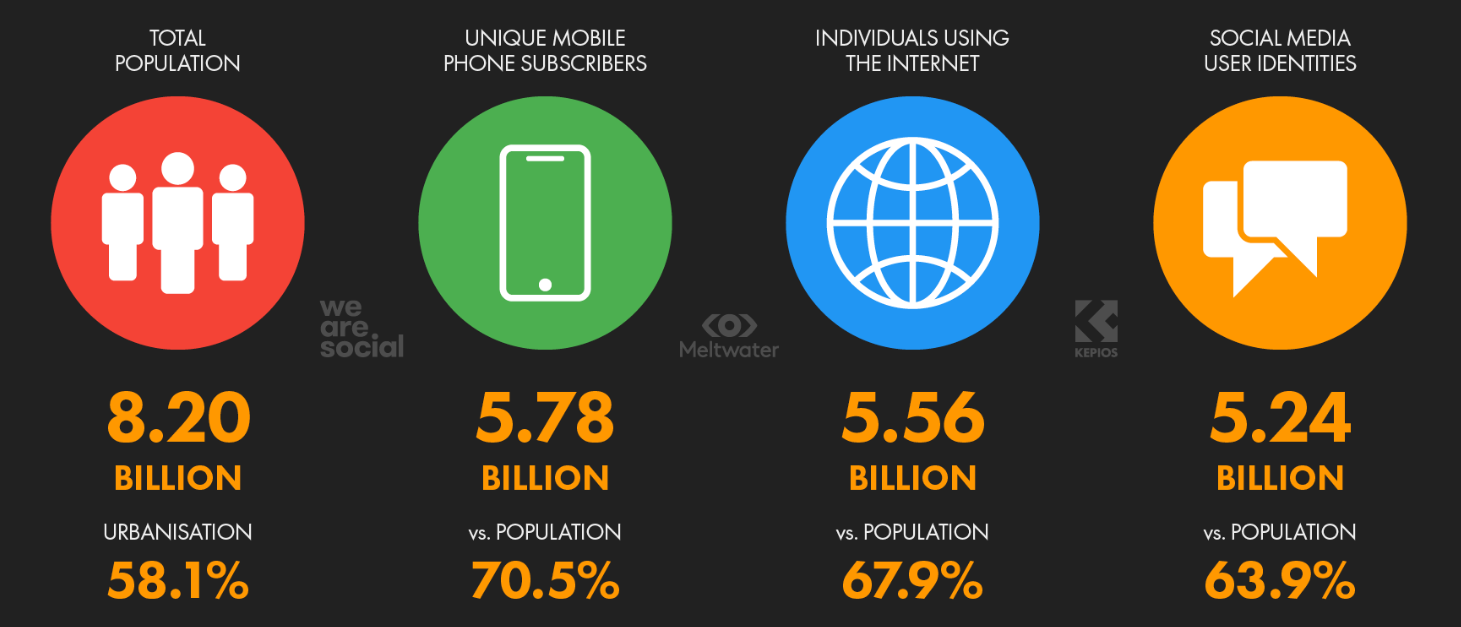
\includegraphics[width=0.7\textwidth]{1/figures/social_media_global.png}
		\caption[Uso global de redes sociales]{Uso global de redes sociales (2025).\\
		Fuente: \textcite{cr_digital2025}.}
		\label{fig:social_media_global}
	\end{center}
\end{figure}

En América Latina, esta tendencia es aún más pronunciada. Según el \textcite{cr_reuters2024}, aproximadamente el 70\% de los usuarios accede a noticias a través de redes sociales, lo que ha incrementado significativamente la influencia de estas plataformas en la formación de percepciones políticas. Tal como se aprecia en la Figura \ref{fig:news_social}, el consumo de información política en entornos digitales ha superado a los medios tradicionales en diversos segmentos de la población.

\begin{figure}[h]
	\begin{center}
		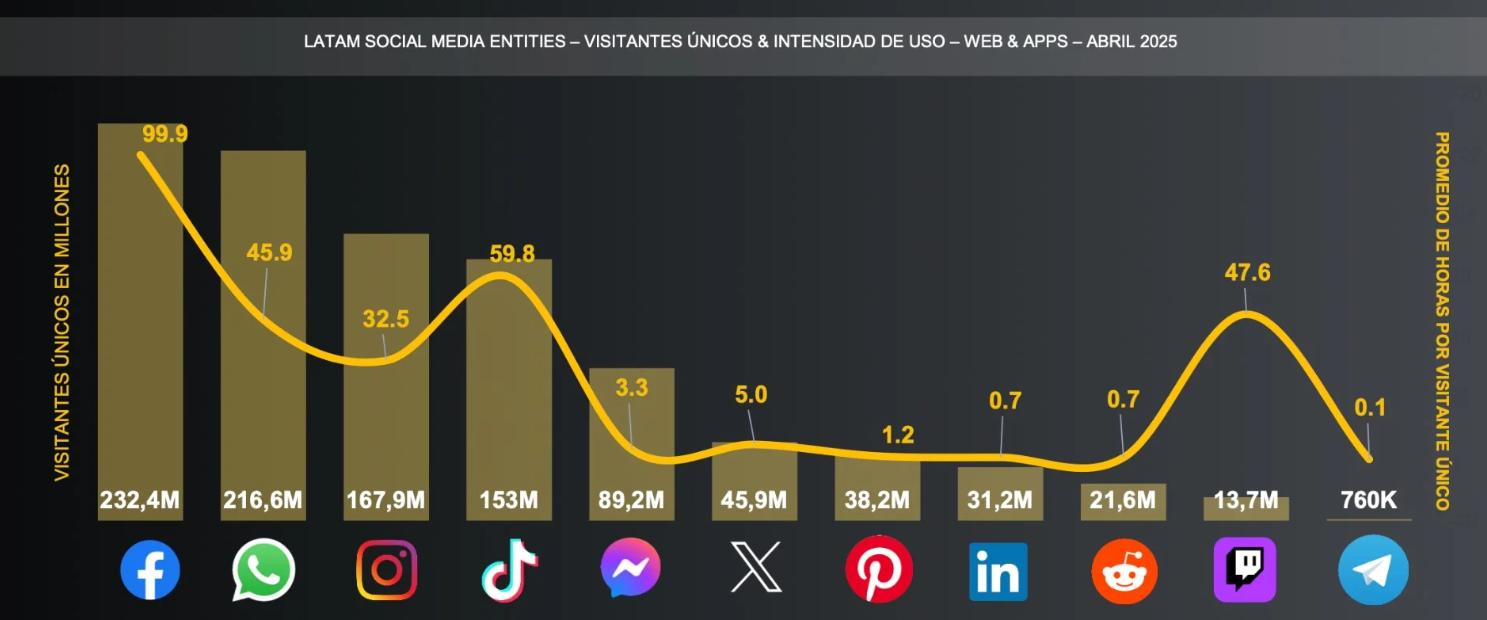
\includegraphics[width=0.7\textwidth]{1/figures/news_social_media.png}
		\caption[Consumo de noticias en redes sociales]{Consumo de noticias a través de redes sociales en América Latina.\\
		Fuente: \textcite{cr_reuters2024}.}
		\label{fig:news_social}
	\end{center}
\end{figure}

En el caso específico del Perú, el acceso a Internet ha alcanzado aproximadamente el 82\% de la población, lo que equivale a más de 28 millones de usuarios conectados, según el Instituto Nacional de Estadística e Informática \parencite{cr_inei2024}. Como se muestra en la Figura \ref{fig:internet_peru}, este alto nivel de penetración digital refuerza la relevancia de analizar la percepción pública en entornos digitales dentro del contexto nacional.

\begin{figure}[h]
	\begin{center}
		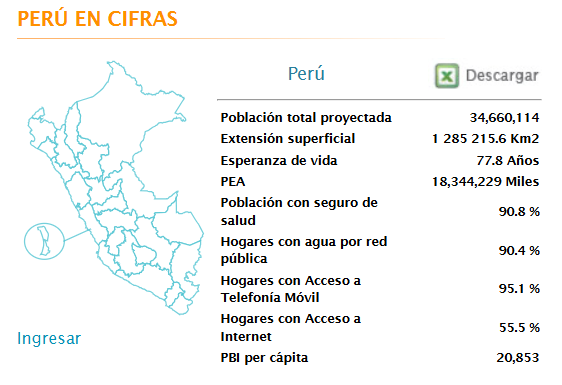
\includegraphics[width=0.65\textwidth]{1/figures/internet_peru.png}
		\caption[Usuarios de internet en Perú]{Acceso a Internet en Perú (2024).\\
		Fuente: \textcite{cr_inei2024}.}
		\label{fig:internet_peru}
	\end{center}
\end{figure}

Sin embargo, este crecimiento también ha generado nuevos desafíos. La sobrecarga informativa, la desinformación y la polarización dificultan la comprensión precisa de la percepción ciudadana en contextos electorales. Tal como señala \textcite{cr_castells2015comunicacion}, la comunicación digital ha dado lugar a una dinámica en la que los ciudadanos no solo consumen información, sino que también la reinterpretan y amplifican, generando múltiples capas de significado.

En este contexto, los métodos tradicionales de análisis de opinión pública, como encuestas o estudios cualitativos, presentan limitaciones importantes debido a su costo, baja frecuencia y limitada capacidad de capturar dinámicas en tiempo real. Por otro lado, los enfoques computacionales existentes suelen centrarse en una sola fuente de datos, como redes sociales, ignorando la diversidad de actores y formatos presentes en el ecosistema digital.

Asimismo, existe una brecha significativa entre el discurso mediático y la percepción ciudadana. Mientras los medios de comunicación establecen agendas informativas, los ciudadanos reaccionan de manera independiente en redes sociales, generando diferencias que no son adecuadamente modeladas por los enfoques actuales. Esta problemática resulta crítica durante procesos electorales, donde la identificación de tendencias, temas relevantes y cambios en la percepción pública es fundamental.

Por otro lado, el avance de los Modelos de Lenguaje de Gran Escala (LLMs) ha abierto nuevas oportunidades para el análisis semántico profundo de grandes volúmenes de datos. Según \textcite{cr_bommasani2021foundation}, estos modelos permiten capturar relaciones complejas en el lenguaje natural, superando las limitaciones de técnicas tradicionales de procesamiento de lenguaje natural.

En consecuencia, se identifica la necesidad de desarrollar un enfoque integral que permita analizar la percepción nacional en contextos electorales mediante la integración de múltiples fuentes de información, el uso de modelos avanzados de lenguaje y la representación estructurada de relaciones mediante grafos de conocimiento.

\section{Formulación del Problema}

\subsection{Problema General}
PG: \newcommand{\ProblemaGeneral}{
¿Es posible analizar la percepción nacional en contextos electorales mediante un sistema de Inteligencia Electoral basado en modelos de lenguaje de gran escala (LLMs), minería de sentimientos y detección dinámica de temas en ecosistemas digitales multi-fuente?
}
\ProblemaGeneral

\subsection{Problemas Específicos}

\newcommand{\Pbone}{¿Qué enfoques existen en la literatura para el análisis de opinión pública mediante inteligencia artificial?}
\newcommand{\Pbtwo}{¿Cómo integrar múltiples fuentes de datos (prensa, redes sociales y plataformas audiovisuales) para representar la percepción pública?}
\newcommand{\Pbthree}{¿Cuál es el impacto del uso de LLMs en el análisis de sentimientos y detección de temas?}
\newcommand{\Pbfour}{¿Cómo modelar las relaciones entre discurso mediático y percepción ciudadana mediante grafos de conocimiento?}

\begin{itemize}
	\item PE1: {\Pbone}
	\item PE2: {\Pbtwo}
	\item PE3: {\Pbthree}
	\item PE4: {\Pbfour}
\end{itemize}


\section{Objetivos de la Investigación}

\subsection{Objetivo General}
OG: \newcommand{\ObjetivoGeneral}{
Analizar la percepción nacional en contextos electorales mediante un sistema basado en LLMs, minería de sentimientos y detección de temas en ecosistemas digitales.
}
\ObjetivoGeneral
\subsection{Objetivos Específicos}

\newcommand{\Objone}{Analizar enfoques existentes en la literatura.}
\newcommand{\Objtwo}{Diseñar una arquitectura multi-fuente.}
\newcommand{\Objthree}{Evaluar el desempeño de LLMs en análisis de sentimientos y detección de temas.}
\newcommand{\Objfour}{Implementar un sistema basado en grafos de conocimiento y GraphRAG.}


\begin{itemize}
	\item OE1: {\Objone}
	\item OE2: {\Objtwo}
	\item OE3: {\Objthree}
	\item OE4: {\Objfour}
\end{itemize}

\section{Hipótesis}

\subsection{Hipótesis General}
HG: \newcommand{\HipotesisGeneral}{
El uso de modelos de lenguaje de gran escala (LLMs) permite analizar con mayor precisión la percepción nacional en entornos digitales multi-fuente durante contextos electorales.
}
\HipotesisGeneral
\subsection{Hipótesis Específicas}

\newcommand{\Hone}{La integración de múltiples fuentes de datos mejora la representatividad de la percepción pública.}
\newcommand{\Htwo}{Los modelos LLMs mejoran la precisión del análisis de sentimientos y detección de temas.}
\newcommand{\Hthree}{El uso de grafos de conocimiento permite modelar relaciones complejas entre actores y discursos.}
\newcommand{\Hfour}{El enfoque GraphRAG mejora la generación de insights en el análisis electoral.}

\begin{itemize}
	\item HE1: \Hone
	\item HE2: \Htwo
	\item HE3: \Hthree
	\item HE4: \Hfour
\end{itemize}


\section{Justificación de la Investigación}

\subsection{Teórica}

La presente investigación se justifica desde una perspectiva teórica debido a la necesidad de integrar enfoques contemporáneos en el análisis de la percepción pública dentro de ecosistemas digitales. Tradicionalmente, los estudios en análisis de opinión y comportamiento electoral se han apoyado en técnicas estadísticas clásicas y métodos de análisis de contenido manual o semiautomático. Sin embargo, el crecimiento exponencial de datos generados en redes sociales y plataformas digitales ha evidenciado limitaciones en dichos enfoques, especialmente en términos de escalabilidad, contextualización semántica y capacidad de adaptación en tiempo real.

En este contexto, el desarrollo de modelos de lenguaje de gran escala (LLMs) ha transformado significativamente el campo del Procesamiento de Lenguaje Natural (NLP), permitiendo una comprensión más profunda del lenguaje humano mediante representaciones contextuales avanzadas \parencite{pr_devlin2019bert, pr_brown2020gpt3}. A su vez, la minería de sentimientos ha evolucionado desde enfoques basados en lexicones hacia modelos más robustos que incorporan aprendizaje profundo, mejorando la precisión en la clasificación de opiniones y emociones \parencite{pr_pang2008opinion}.

Adicionalmente, la incorporación de grafos de conocimiento permite modelar relaciones semánticas complejas entre entidades, facilitando la interpretación estructurada de la información y el descubrimiento de patrones emergentes en grandes volúmenes de datos. En particular, enfoques recientes como GraphRAG combinan capacidades de recuperación de información con razonamiento basado en grafos, ampliando las posibilidades analíticas en sistemas inteligentes.

En este sentido, la presente investigación propone un enfoque integrador que articula LLMs, análisis de sentimientos, modelado de tópicos y grafos de conocimiento, contribuyendo a la literatura mediante una aproximación holística que supera las limitaciones de estudios previos centrados en técnicas aisladas. De esta manera, se aporta al desarrollo teórico de la inteligencia electoral como un campo emergente dentro de la analítica de datos y la ciencia política computacional.

\subsection{Práctica}

Desde el punto de vista práctico, la investigación responde a la creciente necesidad de comprender la percepción ciudadana en contextos electorales de manera oportuna, precisa y escalable. En la actualidad, los procesos electorales están fuertemente influenciados por la dinámica de los ecosistemas digitales, donde plataformas como redes sociales, medios digitales y foros en línea actúan como espacios clave para la formación de opinión pública.

El análisis tradicional de encuestas presenta limitaciones en términos de cobertura, costo y frecuencia de actualización, lo que dificulta capturar cambios dinámicos en la percepción ciudadana. En contraste, el uso de técnicas de minería de datos sobre información generada en tiempo real permite identificar tendencias emergentes, cambios en el sentimiento colectivo y temas de interés prioritario para la población.

En este contexto, la implementación de un sistema basado en LLMs y análisis multi-fuente permitirá procesar grandes volúmenes de datos provenientes de diversas plataformas digitales, generando indicadores relevantes sobre el comportamiento y percepción de los ciudadanos. Esto puede ser de utilidad para diversos actores, como analistas políticos, instituciones públicas, organizaciones de investigación y medios de comunicación, quienes podrán tomar decisiones más informadas basadas en evidencia empírica.

Asimismo, la capacidad de detección dinámica de temas relevantes permite identificar oportunamente eventos críticos, crisis de reputación o cambios en la agenda pública, contribuyendo a una mejor comprensión del entorno político y social.

\subsection{Metodológica}

En el ámbito metodológico, la investigación propone una arquitectura innovadora que integra múltiples técnicas avanzadas de análisis de datos, superando enfoques tradicionales basados en modelos únicos o fuentes de datos limitadas.

En primer lugar, se plantea un enfoque de análisis multi-fuente, que considera la integración de datos provenientes de diversas plataformas digitales, lo cual permite obtener una visión más completa y representativa del ecosistema informacional. En segundo lugar, se incorporan modelos de lenguaje de gran escala (LLMs) para el procesamiento semántico avanzado, facilitando tareas como clasificación de sentimientos, resumen de información y extracción de entidades.

Adicionalmente, se propone el uso de técnicas de modelado de tópicos para la detección automática de temas relevantes, permitiendo identificar patrones emergentes en el discurso público. Este componente se complementa con la construcción de grafos de conocimiento, los cuales modelan relaciones entre actores, temas y eventos, enriqueciendo el análisis con una dimensión estructural.

Finalmente, la integración de estos componentes mediante un enfoque tipo GraphRAG permite combinar capacidades de recuperación de información, razonamiento contextual y análisis estructurado, constituyendo una contribución metodológica significativa en el desarrollo de sistemas de inteligencia electoral basados en inteligencia artificial.

\section{Delimitación del Estudio}

\subsection{Espacial}

La investigación se delimita geográficamente al contexto peruano, con una extensión analítica hacia el ámbito latinoamericano. Esta delimitación responde a la relevancia de los procesos electorales en la región, caracterizados por una alta participación en entornos digitales y una creciente influencia de las redes sociales en la formación de opinión pública.

El enfoque en Perú permite contextualizar el análisis en un entorno específico con características sociopolíticas propias, mientras que la consideración del contexto latinoamericano posibilita la comparación y generalización de resultados en escenarios similares.

\subsection{Temporal}

En términos temporales, la investigación se centra en el análisis de datos recientes provenientes de ecosistemas digitales, priorizando información generada en los últimos años. Esta delimitación permite capturar dinámicas actuales en el comportamiento de los usuarios, así como tendencias emergentes en el uso de plataformas digitales para la expresión de opiniones políticas.

Asimismo, el enfoque en datos recientes es coherente con la naturaleza cambiante del entorno digital, donde los temas de interés y el sentimiento colectivo pueden variar rápidamente en función de eventos coyunturales.

\subsection{Conceptual}

Desde el punto de vista conceptual, la investigación se enfoca en el análisis de la percepción pública mediante técnicas de Procesamiento de Lenguaje Natural (NLP), modelos de lenguaje de gran escala (LLMs) y grafos de conocimiento.

Se consideran conceptos clave como minería de sentimientos, detección de tópicos, análisis semántico y modelado de relaciones entre entidades. Asimismo, se enmarca dentro del campo de la analítica de datos aplicada a la ciencia política, particularmente en el ámbito de la inteligencia electoral.

No se abordan aspectos relacionados con la predicción directa de resultados electorales, sino que el énfasis se encuentra en la comprensión de la percepción ciudadana y la identificación de patrones en el discurso público digital.
%\include{2/marco}
%\chapter{Metodología de la Investigación}
 
\section{Diseño de la investigación}
 
En esta sección se explica cuál fue el diseño, el tipo y el enfoque del trabajo de
investigación, así como también la población, la muestra y la operacionalización de
variables.
 
\subsection{Tipo de la investigación}
 
Para determinar el tipo de la investigación, primero fue necesario definir el actual
trabajo como \textbf{Diseño Experimental} ya que, según \cite{bk_hernandez2014metodologia}
en su libro \citetitle{bk_hernandez2014metodologia}, se pretende establecer el posible
efecto de una causa que se manipula. Dentro de esta categoría se clasifica como
\textbf{Diseño Experimental Puro}, ya que se manipularon intencionalmente una o más
variables independientes —específicamente la configuración del pipeline de análisis con
LLMs— con la finalidad de medir el efecto que estas generan en la variable dependiente:
la exactitud en la clasificación del sentimiento y la coherencia semántica en la detección
de temas relevantes en el ecosistema digital electoral peruano.
 
\subsection{Enfoque de la investigación}
 
El presente trabajo tuvo un \textbf{enfoque cuantitativo} ya que, según
\cite{bk_hernandez2014metodologia} en su libro \citetitle{bk_hernandez2014metodologia},
este enfoque utiliza la recolección de datos para probar hipótesis con base en la medición
numérica y el análisis estadístico, con el fin de establecer pautas de comportamiento y
probar teorías. Esto se refleja en los 10 pasos del proceso cuantitativo descritos por el
anterior autor y que fueron aplicados en la investigación, desde la concepción de la idea
hasta la elaboración del reporte de resultados. En el presente trabajo, las métricas de
exactitud, coherencia temática y latencia de procesamiento permiten evaluar de forma
objetiva el desempeño del sistema de inteligencia electoral propuesto.
 
\subsection{Población}
 
La población fue el conjunto de todas las publicaciones digitales en español relacionadas
con el proceso electoral peruano, generadas en plataformas de redes sociales (X/Twitter),
portales de noticias digitales y canales de YouTube durante el período de campaña
presidencial analizado.
 
\subsection{Muestra}
 
La muestra estuvo conformada por publicaciones recolectadas de tres fuentes de datos
durante el período electoral comprendido entre los meses de enero y junio del año en
curso: (1) artículos y noticias digitales de los principales portales de prensa peruanos;
(2) comentarios de usuarios en los videos de YouTube de los candidatos y programas
periodísticos de cobertura electoral; y (3) tweets y publicaciones de X/Twitter
relacionados con los candidatos presidenciales, filtrados mediante palabras clave
electorales y hashtags de campaña. El criterio de delimitación temporal obedeció a la
necesidad de capturar el período de mayor actividad del ecosistema digital electoral,
excluyendo etapas de baja intensidad que distorsionarían los patrones de sentimiento y
emergencia de temas.
 
\subsection{Operacionalización de variables}
 
En la Tabla \ref{4:table1} se presenta la operacionalización de variables para la
investigación.
 
\begin{longtable}{M{3cm}M{4.2cm}M{3.6cm}M{4.8cm}}
    \caption[Matriz de operacionalización de variables]{Matriz de operacionalización de variables.}
    \label{4:table1}
    \centering
    \small
    \tabularnewline \specialrule{.1em}{.05em}{.05em}
    VARIABLE & DIMENSIÓN & INDICADOR & CÁLCULO \\
    \specialrule{.1em}{.05em}{.05em}
 
    % Variable independiente
    \multirow{8}{3cm}[-5ex]{\centering Independiente: Sistema de Inteligencia Electoral con LLM}
    & \multirow{6}{4.2cm}[-1ex]{\centering Modelo LLM de Análisis}
    & \multicolumn{2}{c}{\centering Configuración del pipeline de análisis} \\
    \cline{3-4}
    & & \multirow{5}{3.6cm}[0ex]{\centering Efectividad del análisis con LLM}
    & Exactitud en clasificación de sentimiento \\
    \cline{4-4}
    & & & Coherencia semántica de temas (C\textsubscript{v}) \\
    \cline{4-4}
    & & & Índice de Sentimiento Neto (ISN) \\
    \cline{4-4}
    & & & Índice de Relevancia Temática (IRT) \\
    \cline{4-4}
    & & & Latencia de procesamiento (ms) \\
    \cline{2-4}
    & Arquitectura del pipeline
    & \multicolumn{2}{c}{\thead{Complejidad e integridad\\del pipeline de procesamiento}} \\
 
    \hline
 
    % Variable dependiente
    \multirow{8}{3cm}[-5ex]{\centering Dependiente: Percepción pública nacional en el ecosistema digital}
    & \multirow{3}{4.2cm}[-2ex]{\centering Sentimiento ciudadano}
    & \multirow{2}{3.6cm}[0ex]{\centering Polaridad de sentimiento}
    & $Positivo: S(d,e) > 0$ \\
    \cline{4-4}
    & & & $Negativo: S(d,e) < 0$ \\
    \cline{3-4}
    & & Intensidad del sentimiento & Score continuo $[-1, 1]$ \\
    \cline{2-4}
    & \multirow{5}{4.2cm}[-2ex]{\centering Conversación digital electoral}
    & \multirow{2}{3.6cm}[0ex]{\centering Metainformación del corpus}
    & Volumen de publicaciones por período \\
    \cline{4-4}
    & & & Distribución por fuente de datos \\
    \cline{3-4}
    & & Temas relevantes & Número y coherencia de temas detectados \\
    \cline{3-4}
    & & \multirow{2}{3.6cm}[0ex]{\centering Evolución temporal}
    & Velocidad de emergencia de temas \\
    \cline{4-4}
    & & & Cambios de sentimiento por evento electoral \\
 
    \specialrule{.1em}{.05em}{.05em}
\end{longtable}
\begin{flushleft}
    \small Fuente: Elaboración propia.
\end{flushleft}
 
El trabajo busca resolver el problema de análisis de percepción pública nacional en
ecosistemas digitales electorales, implementando un pipeline automatizado de inteligencia
electoral que integra análisis de sentimientos con LLMs y detección dinámica de temas
mediante BERTopic sobre un corpus multicanal de publicaciones en español.
 
La variable dependiente —la percepción pública nacional— se operacionaliza a través del
sentimiento expresado en publicaciones digitales hacia cada candidato presidencial,
desagregado por fuente de información, período temporal y tema relevante asociado.
Siguiendo la metodología GraphRAG descrita en la arquitectura del sistema, un mismo
segmento de texto puede expresar sentimientos distintos hacia distintos candidatos, lo que
permite capturar la complejidad real del discurso político ciudadano a nivel de aspecto
(\textit{Aspect-Based Sentiment Analysis}).
 
\section{Técnicas de recolección de datos}
 
Los conjuntos de datos recolectados para la investigación se componen de variables
cuantitativas —como el score continuo de sentimiento $[-1, 1]$, el volumen de
publicaciones por período y la frecuencia de temas— y variables cualitativas —como el
texto de las publicaciones, los fragmentos clave que justifican el sentimiento y las
etiquetas de temas generadas por el LLM—. Para obtener los tres corpus principales, se
siguió el flujo de la Figura \ref{4:fig1}.
 
\begin{figure}[!ht]
    \begin{center}
        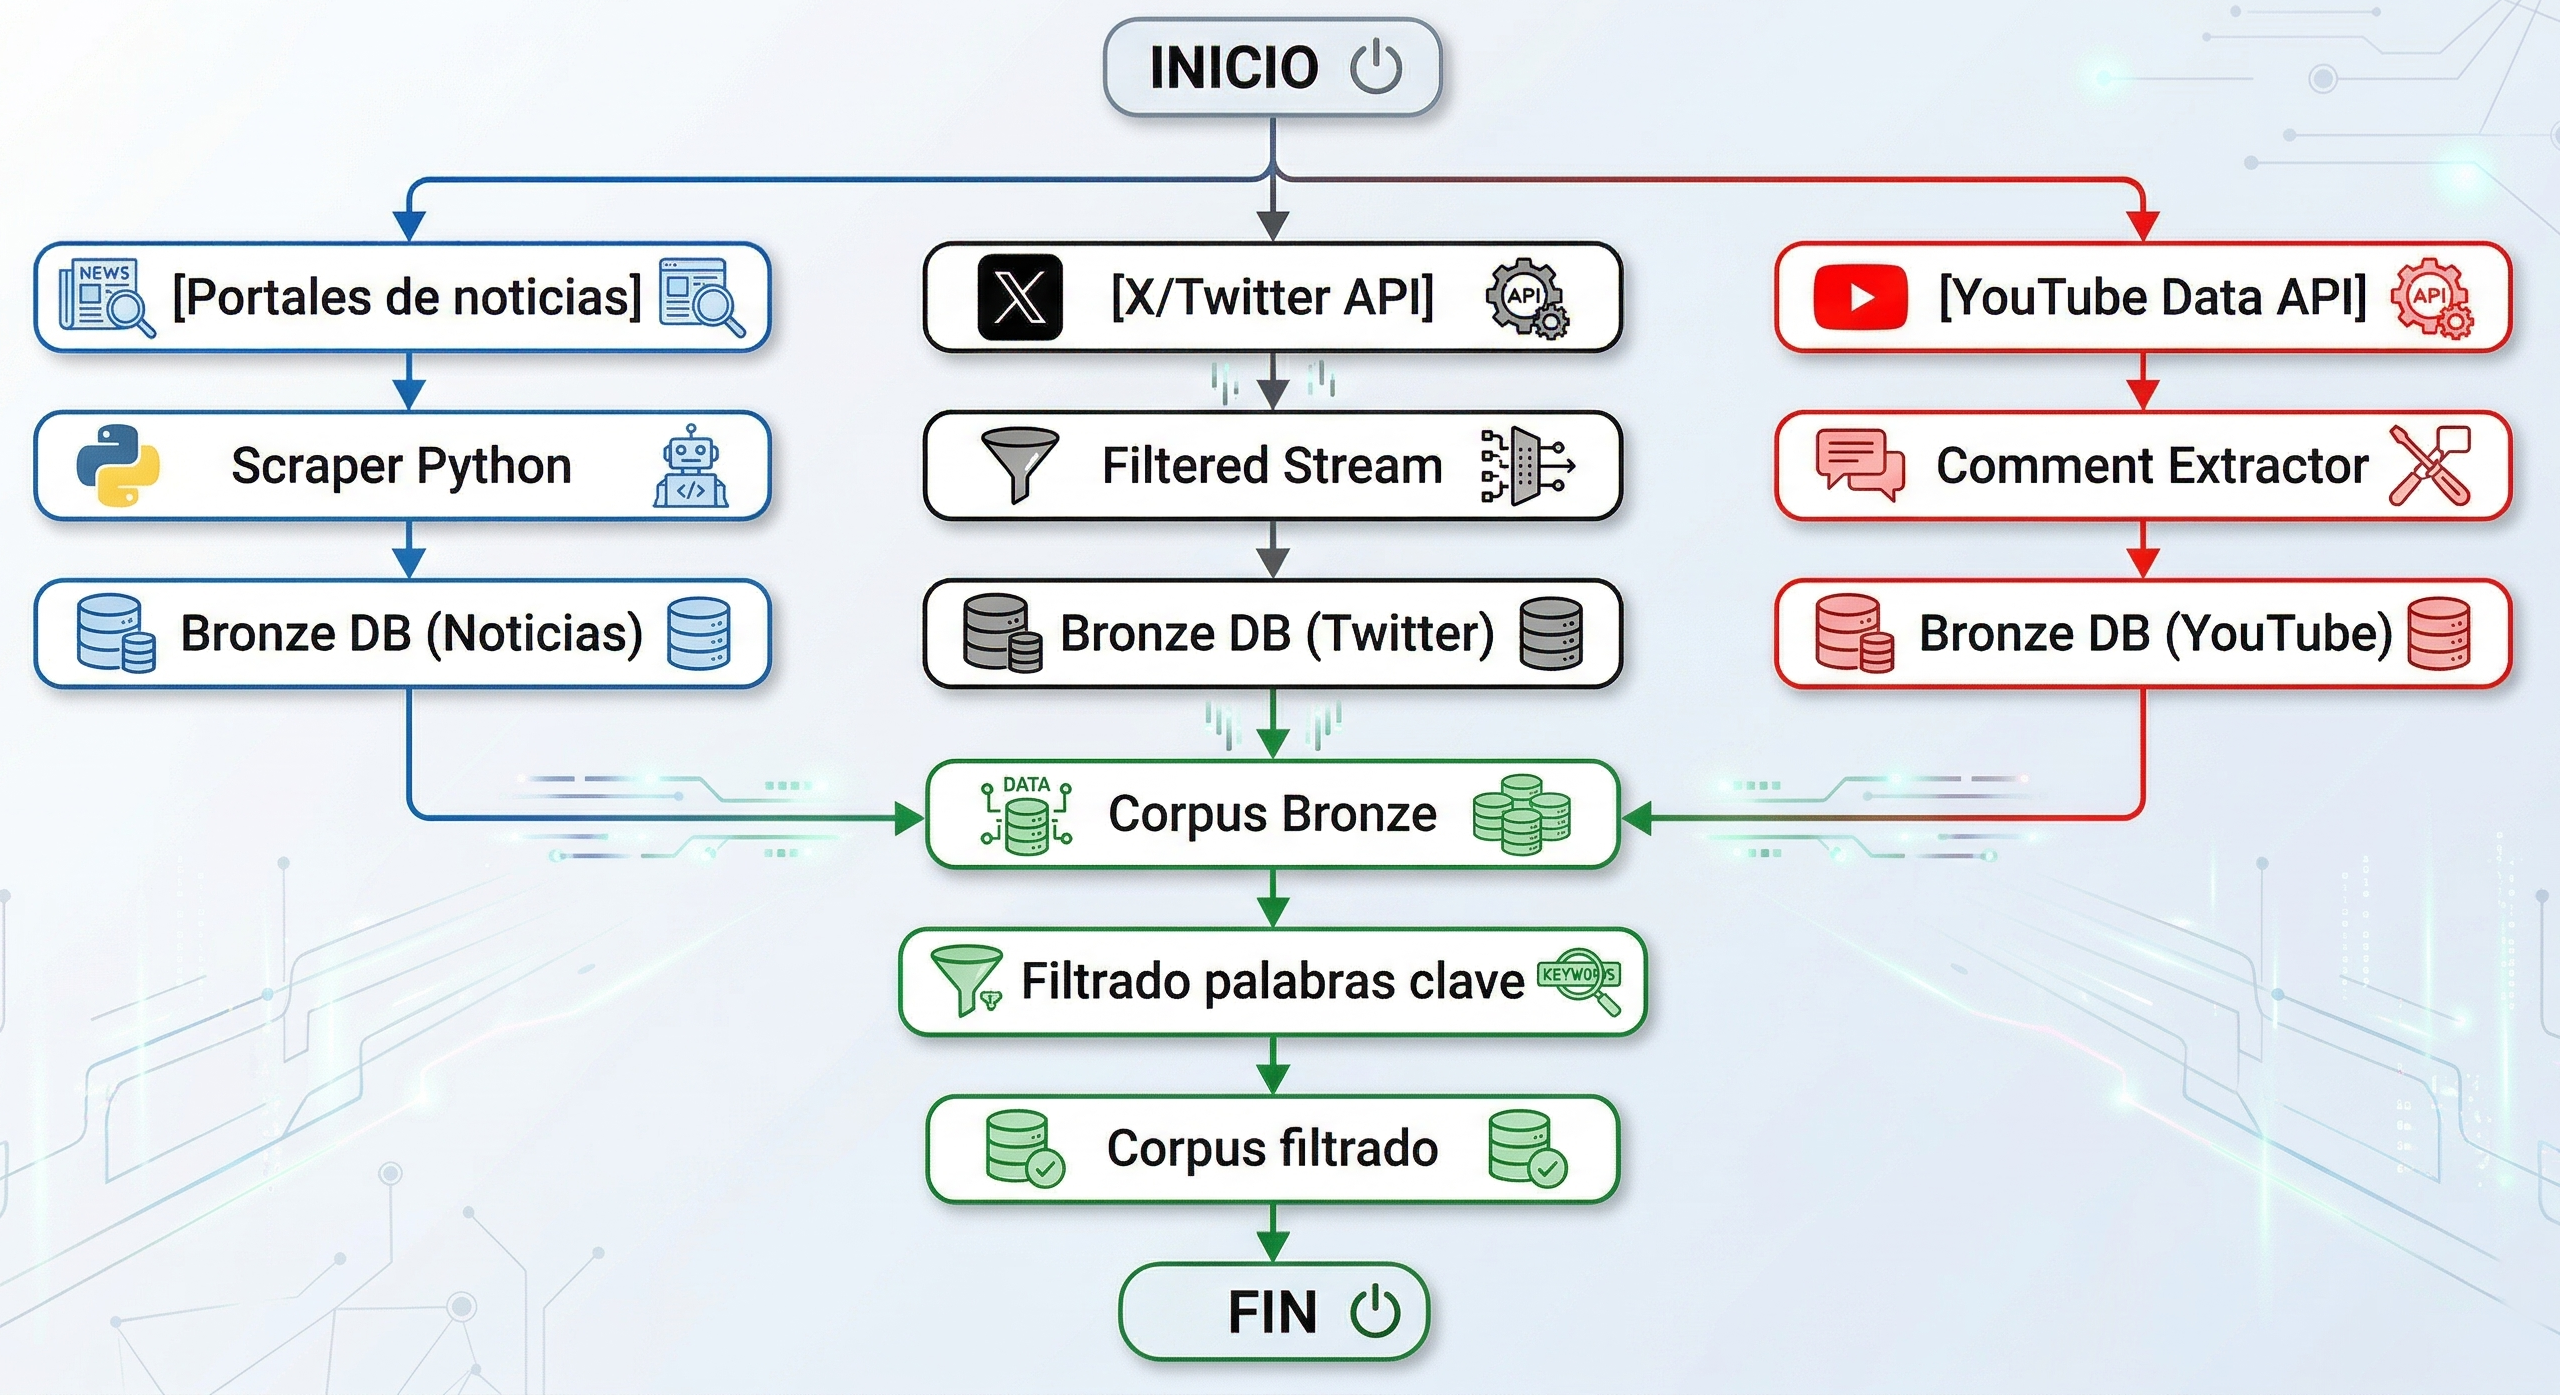
\includegraphics[width=0.90\textwidth]{3/figures/flujo_recoleccion.png}
        \caption[Flujograma de recolección de los conjuntos de datos del corpus electoral]{Flujograma de recolección de los conjuntos de datos del corpus electoral: noticias digitales, comentarios de YouTube y tweets de X/Twitter, con sus respectivos procesos de filtrado y almacenamiento en la capa Bronze de la arquitectura Medallion.\\
            Fuente: Elaboración propia.}
        \label{4:fig1}
    \end{center}
\end{figure}
 
Asimismo, para identificar y filtrar las publicaciones relevantes para el análisis, se
definió un diccionario de palabras clave y aliases electorales que incluye los nombres
completos, apodos, partidos y hashtags de los candidatos presidenciales en liza, así como
términos relacionados con los principales temas de la campaña: economía, seguridad,
educación, salud, corrupción y gobernabilidad.
 
\section{Técnicas para el procesamiento y análisis de la información}
 
\subsection{Metodología de implementación de la solución}
 
Como se explicó en el Capítulo II del presente trabajo, dentro de los sistemas de
analítica de negocio, Big Data y Minería de Datos, las tres metodologías más usadas son
CRISP-DM, SEMMA y KDD \parencite{tec_braulio2015metodologiasdm}. Para elegir la
metodología de implementación, se elaboró la Tabla \ref{4:table2} con el fin de comparar
las utilizadas por los autores en los antecedentes de esta investigación.
 
\vspace{2ex}
\begingroup
\renewcommand\arraystretch{0.3}
\begin{longtable}{M{3cm}M{2.5cm}M{2.5cm}M{6cm}}
    \caption[Cuadro comparativo para la selección de la metodología]{Cuadro comparativo para la selección de la metodología de implementación.}
    \label{4:table2}
    \footnotesize
    \centering
    \small
    \tabularnewline \specialrule{.1em}{.05em}{.05em}
    Metodología & Cantidad de referencias & Número de pasos & Nombre de los pasos \\
    \specialrule{.1em}{.05em}{.05em}
    {CRISP-DM}
    & 2
    & 6
    & \setlist{nolistsep}
    \begin{itemize}[label={--},nosep,noitemsep,leftmargin=*,topsep=0pt,partopsep=0pt]
        \item Comprensión del negocio.
        \item Comprensión de los datos.
        \item Preparación de los datos.
        \item Modelado.
        \item Evaluación.
        \item Despliegue.
    \end{itemize}
    \\
    \hline
    {Grupo A}
    & 2
    & 6
    & \setlist{nolistsep}
    \begin{itemize}[label={--},nosep,noitemsep,leftmargin=*,topsep=0pt,partopsep=0pt]
        \item Formulación del problema.
        \item Recolección de datos multicanal.
        \item Preprocesamiento de texto.
        \item Análisis con LLM.
        \item Evaluación.
        \item Despliegue.
    \end{itemize}
    \\
    \hline
    {Grupo B}
    & 2
    & 5
    & \setlist{nolistsep}
    \begin{itemize}[label={--},nosep,noitemsep,leftmargin=*,topsep=0pt,partopsep=0pt]
        \item Recolección de datos.
        \item Preprocesamiento y filtrado.
        \item Análisis de sentimientos.
        \item Detección de temas.
        \item Evaluación.
    \end{itemize}
    \\
    \hline
    {Grupo C}
    & 2
    & 5
    & \setlist{nolistsep}
    \begin{itemize}[label={--},nosep,noitemsep,leftmargin=*,topsep=0pt,partopsep=0pt]
        \item Formulación del problema.
        \item Recolección de datos.
        \item Preprocesamiento de datos.
        \item Modelado y análisis.
        \item Evaluación.
    \end{itemize}
    \\
    \hline
    {Grupo D}
    & 1
    & 4
    & \setlist{nolistsep}
    \begin{itemize}[label={--},nosep,noitemsep,leftmargin=*,topsep=0pt,partopsep=0pt]
        \item Recolección de datos.
        \item Preprocesamiento.
        \item Análisis LLM y clustering.
        \item Evaluación.
    \end{itemize}
    \\
    \specialrule{.1em}{.05em}{.05em}
\end{longtable}
\endgroup
\begin{flushleft}
    \small Fuente: Elaboración propia.
\end{flushleft}
 
De las tres metodologías mencionadas por \citeauthor{tec_braulio2015metodologiasdm},
la mayoría de los antecedentes revisados siguen secuencias de actividades comprendidas
dentro de CRISP-DM, incluyendo fases de comprensión del negocio, recolección y
preparación de datos, modelado y evaluación. Además, las siguientes características de la
literatura influyeron en la elección de la metodología CRISP-DM para el presente trabajo:
 
\begin{itemize}
    \item La metodología contempla entre sus fases la comprensión del negocio además
    de la parte técnica. Esta fase es crucial ya que en ella se define el problema a resolver
    —la falta de un sistema de análisis automatizado de percepción pública electoral en
    tiempo real— y se establecen los objetivos del sistema.
 
    \item Ayuda a los responsables del proyecto en la planificación y toma de decisiones
    (fase de Despliegue) a partir de los resultados obtenidos, convirtiendo los indicadores
    del sistema en oportunidades para mejorar la campaña de inteligencia electoral.
 
    \item Evalúa en todo el proceso los datos y configuraciones del modelo con el fin de
    construir el mejor pipeline. Estas evaluaciones son importantes para interpretar los
    resultados y tomar decisiones sobre la arquitectura del sistema.
 
    \item A diferencia de SEMMA, que comienza directamente con el muestreo sin hacer
    hincapié en la comprensión del contexto, y de KDD, cuyo enfoque es más técnico y
    orientado a métricas sin considerar el entorno del negocio, CRISP-DM contempla
    explícitamente la formulación del problema, presente en el actual trabajo.
\end{itemize}
 
Cada una de las fases de la metodología seleccionada, adaptada al contexto de la
inteligencia electoral con LLMs, se detalla en la Figura \ref{4:fig2}.
 
\begin{figure}[!ht]
    \begin{center}
        \includegraphics[width=1\textwidth]{3/figures/metodologia_crispdm.png}
        \caption[Metodología CRISP-DM adaptada al sistema de inteligencia electoral con LLMs]{Metodología CRISP-DM adaptada al sistema de inteligencia electoral con LLMs, mostrando las seis fases, su carácter iterativo y los entregables de cada etapa.\\
            Fuente: Elaboración propia.}
        \label{4:fig2}
    \end{center}
\end{figure}
 
Durante el proceso de implementación de la metodología, se definió construir un pipeline
de análisis multicanal que integra análisis de sentimientos con LLMs, detección dinámica
de temas con BERTopic y un grafo de conocimiento con Neo4j, arquitectura denominada
\textbf{GraphRAG Electoral}. De acuerdo a la literatura de los antecedentes revisados,
se analizaron las siguientes posibles fuentes de datos a incorporar:
 
\begin{itemize}
    \item \textbf{Noticias digitales}: \cite{pr_alvarez2023llm_political}, \cite{pr_mendonca2025bertopic_political}, \cite{pr_alvi2023twitter_election_review}.
    \item \textbf{Publicaciones en X/Twitter}: \cite{pr_gujral2024llm_elections}, \cite{pr_alvi2023twitter_election_review}, \cite{pr_mendonca2025bertopic_political}.
    \item \textbf{Comentarios de YouTube}: \cite{pr_chen2024combating_misinformation}.
    \item \textbf{Datos de encuestas electorales}: \cite{pr_gujral2024llm_elections}.
\end{itemize}
 
De las anteriores fuentes, los datos de encuestas electorales no fueron incluidos en el
pipeline principal de procesamiento ya que se utilizan exclusivamente como conjunto de
validación para calibrar los indicadores del sistema, y no como datos de entrada para el
análisis de sentimientos. Finalmente, fueron seleccionadas las tres fuentes principales
—noticias digitales, X/Twitter y comentarios de YouTube— cuya arquitectura de
recolección, procesamiento y análisis se detalla en las subsecciones siguientes.
 
El marco de trabajo del sistema propuesto, denominado \textbf{Pipeline GraphRAG
Electoral}, se estructura según la arquitectura Medallion en tres capas de datos
(Bronze, Silver y Gold) y cinco etapas de procesamiento, como se aprecia en la
Figura \ref{4:fig3}.
 
\begin{figure}[!ht]
    \begin{center}
        \includegraphics[width=0.92\textwidth]{3/figures/framework_graphrag.png}
        \caption[Marco de trabajo del Pipeline GraphRAG Electoral propuesto]{Marco de trabajo del Pipeline GraphRAG Electoral: arquitectura Medallion con tres capas de datos (Bronze, Silver, Gold) y cinco etapas de procesamiento desde la ingesta hasta la generación de indicadores de percepción pública.\\
            Fuente: Elaboración propia.}
        \label{4:fig3}
    \end{center}
\end{figure}
 
\subsubsection{Comprensión del negocio}
 
En la primera fase, se definió el problema a partir de comprender el contexto del proceso
electoral peruano y la necesidad de un sistema automatizado de inteligencia electoral. Las
actividades y tareas de esta fase se presentan en la Tabla \ref{4:table3}.
 
\vspace{2ex}
\begingroup
\renewcommand\arraystretch{0.3}
\begin{longtable}{m{5cm}m{5cm}M{5cm}}
    \caption[Actividades de la fase Comprensión del negocio]{Actividades de la fase Comprensión del negocio.}
    \label{4:table3}
    \footnotesize
    \small
    \tabularnewline \specialrule{.1em}{.05em}{.05em}
    \centering Actividades & \centering Descripción & Tareas \\
    \specialrule{.1em}{.05em}{.05em}
    Definir problema, objetivos e hipótesis.
    & Definición del problema central, los objetivos generales y específicos, y las hipótesis de investigación.
    & \setlist{nolistsep}
    \begin{itemize}[label={--},nosep,noitemsep,leftmargin=*,topsep=0pt,partopsep=0pt]
        \item Identificar la brecha en el análisis de percepción electoral digital.
        \item Definir los objetivos del sistema de inteligencia electoral.
        \item Formular las hipótesis del trabajo.
    \end{itemize}
    \\
    \hline
    Desarrollar la literatura de la investigación.
    & Revisión de antecedentes y trabajos previos sobre análisis de sentimientos político, LLMs y detección de temas.
    & \setlist{nolistsep}
    \begin{itemize}[label={--},nosep,noitemsep,leftmargin=*,topsep=0pt,partopsep=0pt]
        \item Buscar publicaciones académicas sobre LLMs en contextos electorales.
        \item Buscar material sobre BERTopic y GraphRAG aplicado a datos políticos.
    \end{itemize}
    \\
    \hline
    Definir metodología y arquitectura del sistema.
    & Selección de la metodología de implementación y diseño de la arquitectura del pipeline.
    & \setlist{nolistsep}
    \begin{itemize}[label={--},nosep,noitemsep,leftmargin=*,topsep=0pt,partopsep=0pt]
        \item Evaluar metodologías de la literatura.
        \item Seleccionar la metodología CRISP-DM.
        \item Diseñar la arquitectura Medallion del sistema.
    \end{itemize}
    \\
    \specialrule{.1em}{.05em}{.05em}
\end{longtable}
\endgroup
\begin{flushleft}
    \small Fuente: Elaboración propia.
\end{flushleft}
 
\textbf{Actividad 1: Definir problema, objetivos e hipótesis}
 
En esta actividad se detalla cómo se identificó la brecha existente en el análisis automatizado de la percepción pública electoral digital en el Perú, se formularon los objetivos de la investigación y se plantearon las hipótesis que guían el trabajo experimental.
 
\textbf{Entregable}: Problema, objetivos e hipótesis definidos.
 
\textbf{Actividad 2: Desarrollar la literatura de la investigación}
 
A partir de los objetivos definidos, se realizó la búsqueda de antecedentes académicos relacionados con el uso de LLMs en contextos electorales, minería de sentimientos político en español, detección dinámica de temas con BERTopic y sistemas GraphRAG. Se elaboró el marco teórico y conceptual descritos en el Capítulo II del presente trabajo.
 
\textbf{Entregable}: Marco teórico, antecedentes y conceptos operacionales de la investigación.
 
\textbf{Actividad 3: Definir metodología y arquitectura del sistema}
 
Luego de revisar los antecedentes y comparar las metodologías utilizadas por cada autor, se seleccionó CRISP-DM como metodología de implementación y se diseñó la arquitectura Medallion del pipeline GraphRAG Electoral.
 
\textbf{Entregable}: Metodología de implementación y arquitectura del sistema.
 
\subsubsection{Comprensión de los datos}
 
La segunda fase abarcó la recolección y el análisis estadístico exploratorio del corpus
electoral multicanal. Los datos utilizados comprenden publicaciones de tres fuentes
principales recolectadas durante el período de campaña presidencial. La lista de
actividades y tareas se presenta en la Tabla \ref{4:table4}.
 
\vspace{2ex}
\begingroup
\renewcommand\arraystretch{0.3}
\begin{longtable}{m{4cm}m{5.5cm}M{5.5cm}}
    \caption[Actividades de la fase Comprensión de los datos]{Actividades de la fase Comprensión de los datos.}
    \label{4:table4}
    \footnotesize
    \small
    \tabularnewline \specialrule{.1em}{.05em}{.05em}
    \centering Actividades & \centering Descripción & Tareas \\
    \specialrule{.1em}{.05em}{.05em}
    Construir corpus de noticias digitales.
    & Construcción del corpus de artículos y titulares de los principales portales de prensa peruanos (capa Bronze).
    & \setlist{nolistsep}
    \begin{itemize}[label={--},nosep,noitemsep,leftmargin=*,topsep=0pt,partopsep=0pt]
        \item Diseñar scrapers para portales de noticias objetivo.
        \item Recolectar artículos con URL, fecha, titular y texto.
        \item Almacenar datos crudos en capa Bronze.
    \end{itemize}
    \\
    \hline
    Construir corpus de X/Twitter.
    & Construcción del corpus de tweets relacionados con los candidatos presidenciales mediante la API de X.
    & \setlist{nolistsep}
    \begin{itemize}[label={--},nosep,noitemsep,leftmargin=*,topsep=0pt,partopsep=0pt]
        \item Configurar conexión con la API Filtered Stream de X.
        \item Definir palabras clave, hashtags y cuentas de interés.
        \item Almacenar tweets con metadatos en capa Bronze.
    \end{itemize}
    \\
    \hline
    Construir corpus de YouTube.
    & Construcción del corpus de comentarios de usuarios en videos electorales de YouTube.
    & \setlist{nolistsep}
    \begin{itemize}[label={--},nosep,noitemsep,leftmargin=*,topsep=0pt,partopsep=0pt]
        \item Identificar videos electorales mediante YouTube Data API.
        \item Recolectar comentarios con ID de usuario y fecha.
        \item Almacenar comentarios crudos en capa Bronze.
    \end{itemize}
    \\
    \hline
    Realizar análisis exploratorio del corpus.
    & Análisis estadístico y exploratorio de las variables del corpus para cada fuente de datos.
    & \setlist{nolistsep}
    \begin{itemize}[label={--},nosep,noitemsep,leftmargin=*,topsep=0pt,partopsep=0pt]
        \item Describir distribución temporal y por fuente.
        \item Analizar longitud de textos y vocabulario.
        \item Identificar candidatos más mencionados.
    \end{itemize}
    \\
    \specialrule{.1em}{.05em}{.05em}
\end{longtable}
\endgroup
\begin{flushleft}
    \small Fuente: Elaboración propia.
\end{flushleft}
 
\textbf{Actividad 1: Construir corpus de noticias digitales}
 
De acuerdo a la Figura \ref{4:fig1}, en esta actividad se construyó el corpus de artículos de noticias digitales mediante scrapers diseñados en Python para los portales de prensa peruanos seleccionados. El proceso de recolección siguió el flujo de la Figura \ref{4:fig4}.
 
\begin{figure}[!ht]
    \begin{center}
        \includegraphics[width=0.80\textwidth]{3/figures/flujo_scraping_noticias.png}
        \caption[Proceso de recolección del corpus de noticias digitales]{Proceso de recolección del corpus de noticias digitales: desde la identificación de portales objetivo hasta el almacenamiento en la capa Bronze de la arquitectura Medallion.\\
            Fuente: Elaboración propia.}
        \label{4:fig4}
    \end{center}
\end{figure}
 
\textbf{Entregable}: Corpus de noticias digitales con URL, fecha, portal de origen, titular y texto completo del artículo.
 
\textbf{Actividad 2: Construir corpus de X/Twitter}
 
Una vez configurada la conexión con la API Filtered Stream de X, se definió el conjunto de palabras clave, hashtags y cuentas de candidatos que activan la captura en tiempo real. El proceso de recolección se realizó según el flujo de la Figura \ref{4:fig5}.
 
\begin{figure}[!ht]
    \begin{center}
        \includegraphics[width=0.80\textwidth]{3/figures/flujo_api_twitter.png}
        \caption[Proceso de recolección del corpus de X/Twitter mediante API Filtered Stream]{Proceso de recolección del corpus de X/Twitter: configuración de reglas de filtrado, captura en streaming y almacenamiento con metadatos en capa Bronze.\\
            Fuente: Elaboración propia.}
        \label{4:fig5}
    \end{center}
\end{figure}
 
\textbf{Entregable}: Corpus de tweets con ID, texto, fecha, número de retweets y menciones a candidatos.
 
\textbf{Actividad 3: Construir corpus de YouTube}
 
Mediante la YouTube Data API, se identificaron los videos electorales más relevantes y se recolectaron sus comentarios de usuarios, excluyendo los publicados por los propios canales de los candidatos para evitar sesgo en la muestra ciudadana. El proceso se detalla en la Figura \ref{4:fig6}.
 
\begin{figure}[!ht]
    \begin{center}
        \includegraphics[width=0.80\textwidth]{3/figures/flujo_youtube_comentarios.png}
        \caption[Proceso de recolección del corpus de comentarios de YouTube]{Proceso de extracción de comentarios de usuarios en videos electorales de YouTube, desde la identificación de videos relevantes hasta el almacenamiento en capa Bronze.\\
            Fuente: Elaboración propia.}
        \label{4:fig6}
    \end{center}
\end{figure}
 
\textbf{Entregable}: Corpus de comentarios de YouTube con ID de video, texto del comentario, fecha y número de likes.
 
\textbf{Actividad 4: Realizar análisis exploratorio del corpus}
 
En esta actividad se realizó el análisis estadístico descriptivo de los tres corpus recolectados: distribución temporal de publicaciones, longitud promedio de textos, distribución de menciones por candidato y por fuente, y análisis del vocabulario electoral dominante mediante nubes de palabras.
 
\textbf{Entregable}: Gráficos estadísticos y descriptivos del corpus por fuente de datos.
 
\subsubsection{Preparación de los datos}
 
En la tercera fase, los datos crudos de la capa Bronze se transformaron en la capa Silver
mediante un conjunto de procesos de limpieza, normalización y enriquecimiento. Las
actividades de esta etapa se detallan en la Tabla \ref{4:table5}.
 
\vspace{2ex}
\begingroup
\renewcommand\arraystretch{0.3}
\begin{longtable}{m{5cm}m{5cm}M{5cm}}
    \caption[Actividades de la fase Preparación de los datos]{Actividades de la fase Preparación de los datos.}
    \label{4:table5}
    \footnotesize
    \small
    \tabularnewline \specialrule{.1em}{.05em}{.05em}
    \centering Actividades & \centering Descripción & Tareas \\
    \specialrule{.1em}{.05em}{.05em}
    Limpiar y normalizar el corpus.
    & Preprocesamiento textual de las publicaciones de las tres fuentes para su análisis con LLM.
    & \setlist{nolistsep}
    \begin{itemize}[label={--},nosep,noitemsep,leftmargin=*,topsep=0pt,partopsep=0pt]
        \item Eliminar spam, bots y publicaciones duplicadas.
        \item Normalizar caracteres especiales, emojis y URLs.
        \item Detectar y filtrar publicaciones en idiomas distintos al español.
    \end{itemize}
    \\
    \hline
    Segmentar el corpus para análisis.
    & División de textos largos en segmentos procesables por el LLM respetando la ventana de contexto.
    & \setlist{nolistsep}
    \begin{itemize}[label={--},nosep,noitemsep,leftmargin=*,topsep=0pt,partopsep=0pt]
        \item Definir tamaño máximo de segmento en tokens.
        \item Implementar segmentación con superposición de contexto.
        \item Registrar relación documento-segmento en base de datos.
    \end{itemize}
    \\
    \hline
    Construir diccionario de aliases electorales.
    & Creación del diccionario de names, apodos y aliases de candidatos para el filtrado con Aho-Corasick.
    & \setlist{nolistsep}
    \begin{itemize}[label={--},nosep,noitemsep,leftmargin=*,topsep=0pt,partopsep=0pt]
        \item Recopilar nombres completos y apodos de candidatos.
        \item Incluir nombres de partidos y lemas de campaña.
        \item Construir el autómata Aho-Corasick para búsqueda eficiente.
    \end{itemize}
    \\
    \specialrule{.1em}{.05em}{.05em}
\end{longtable}
\endgroup
\begin{flushleft}
    \small Fuente: Elaboración propia.
\end{flushleft}
 
\textbf{Actividad 1: Limpiar y normalizar el corpus}
 
En esta actividad se aplicó un pipeline de preprocesamiento textual sobre los tres corpus de la capa Bronze. El proceso incluyó la eliminación de spam y cuentas de bots identificadas mediante patrones de comportamiento, la normalización de emojis (convertidos a texto descriptivo), la eliminación de URLs y menciones de usuario, y la detección automática de idioma mediante la librería \texttt{langdetect} para conservar únicamente publicaciones en español.
 
\textbf{Entregable}: Corpus limpio y normalizado, listo para análisis con LLM.
 
\textbf{Actividad 2: Segmentar el corpus para análisis}
 
Dado que los artículos de noticias superan en longitud la ventana de contexto del LLM utilizado, se implementó un proceso de segmentación con superposición que divide cada documento en segmentos de máximo 512 tokens con una superposición de 50 tokens entre segmentos consecutivos, preservando el contexto necesario para el análisis de sentimientos a nivel de aspecto.
 
\textbf{Entregable}: Tabla de segmentos con relación uno-a-muchos hacia la tabla de documentos originales (capa Silver).
 
\textbf{Actividad 3: Construir diccionario de aliases electorales}
 
Se construyó el diccionario de aliases que alimenta el autómata Aho-Corasick descrito en el pipeline. Este diccionario incluye los nombres completos, apodos, partidos políticos y lemas de campaña de todos los candidatos presidenciales, permitiendo detectar menciones implícitas y coloquiales que un buscador de texto exacto no capturaría. Este paso es fundamental para garantizar que el LLM solo analice segmentos que efectivamente contienen referencias a candidatos, reduciendo el costo computacional en un factor proporcional al número de aliases registrados.
 
\textbf{Entregable}: Diccionario de aliases y autómata Aho-Corasick compilado.
 
\subsubsection{Modelamiento}
 
Al concluir la preparación de los datos, los segmentos del corpus enriquecido fueron
procesados por el pipeline de análisis con LLMs. Las actividades de esta fase se detallan
en la Tabla \ref{4:table6}.
 
\vspace{2ex}
\begingroup
\renewcommand\arraystretch{0.3}
\begin{longtable}{m{4.6cm}m{4.9cm}M{5.5cm}}
    \caption[Actividades de la fase Modelamiento]{Actividades de la fase Modelamiento.}
    \label{4:table6}
    \footnotesize
    \small
    \tabularnewline \specialrule{.1em}{.05em}{.05em}
    \centering Actividades & \centering Descripción & Tareas \\
    \specialrule{.1em}{.05em}{.05em}
    Desarrollar módulo de análisis de sentimientos con LLM.
    & Implementación del análisis de sentimientos a nivel de aspecto mediante prompts diseñados para el contexto electoral peruano.
    & \setlist{nolistsep}
    \begin{itemize}[label={--},nosep,noitemsep,leftmargin=*,topsep=0pt,partopsep=0pt]
        \item Diseñar prompt de análisis con estructura role-context-task-format.
        \item Implementar llamadas a la API del LLM con respuesta JSON estructurada.
        \item Validar outputs y gestionar errores de parsing.
    \end{itemize}
    \\
    \hline
    Desarrollar módulo de detección dinámica de temas.
    & Implementación del pipeline BERTopic para clustering semántico de temas electorales.
    & \setlist{nolistsep}
    \begin{itemize}[label={--},nosep,noitemsep,leftmargin=*,topsep=0pt,partopsep=0pt]
        \item Generar embeddings con Sentence-BERT multilingüe.
        \item Reducir dimensionalidad con UMAP.
        \item Aplicar HDBSCAN para clustering inductivo.
        \item Etiquetar clusters con LLM mediante c-TF-IDF.
    \end{itemize}
    \\
    \hline
    Construir grafo de conocimiento electoral.
    & Implementación del grafo Neo4j con nodos y relaciones del ecosistema electoral digital.
    & \setlist{nolistsep}
    \begin{itemize}[label={--},nosep,noitemsep,leftmargin=*,topsep=0pt,partopsep=0pt]
        \item Definir esquema de nodos (Candidato, Tema, Fuente, Periodo, Evento).
        \item Implementar jobs de agregación semanal con MERGE idempotente.
        \item Calcular relaciones MENCIONA, CO\_OCURRE, CUBRE y REACCIONA\_A.
    \end{itemize}
    \\
    \hline
    Implementar sistema GraphRAG para consultas.
    & Desarrollo del módulo de consulta en lenguaje natural sobre el grafo de conocimiento electoral.
    & \setlist{nolistsep}
    \begin{itemize}[label={--},nosep,noitemsep,leftmargin=*,topsep=0pt,partopsep=0pt]
        \item Inyectar schema del grafo al contexto del LLM.
        \item Implementar traducción de preguntas en español a consultas Cypher.
        \item Validar respuestas con evidencia textual de los documentos originales.
    \end{itemize}
    \\
    \specialrule{.1em}{.05em}{.05em}
\end{longtable}
\endgroup
\begin{flushleft}
    \small Fuente: Elaboración propia.
\end{flushleft}
 
\textbf{Actividad 1: Desarrollar módulo de análisis de sentimientos con LLM}
 
En esta actividad se diseñó el prompt de análisis de sentimientos a nivel de aspecto y se
implementó el módulo de llamadas a la API del LLM. El prompt sigue la estructura de
cinco componentes (rol, contexto, instrucción, formato y ejemplos few-shot) descrita en el
marco conceptual, y extrae en una sola llamada por segmento: candidatos detectados,
método de detección, nivel de confianza, score de sentimiento en escala $[-1, 1]$,
fragmento clave que justifica el sentimiento, temas identificados y relaciones entre temas.
Para la selección del LLM, se realizó un benchmarking sobre las propuestas de los
autores de los antecedentes:
 
\begin{itemize}
    \item \textbf{Gemini (Google)}: \cite{pr_alvarez2023llm_political}, arquitectura del HTML de metodología adjunto.
    \item \textbf{GPT-4 (OpenAI)}: \cite{pr_gujral2024llm_elections}, \cite{pr_chen2024combating_misinformation}.
    \item \textbf{Llama 2 (Meta, código abierto)}: \cite{pr_gujral2024llm_elections}.
    \item \textbf{mBERT / XLM-RoBERTa (modelos encoder)}: \cite{pr_alvi2023twitter_election_review}.
\end{itemize}
 
De acuerdo a los resultados de los antecedentes, los modelos generativos (GPT-4, Gemini)
superan a los modelos encoder en precisión contextual para análisis de sentimientos
político en español, especialmente en el manejo de ironía, sarcasmo y ambigüedad
semántica. Dado que la investigación requiere análisis en tiempo real con respuestas JSON
estructuradas, se seleccionó la API de Gemini Flash como modelo principal por su relación
entre capacidad y latencia, y GPT-4o como modelo de validación para los experimentos de
evaluación.
 
\textbf{Entregable}: Módulo de análisis de sentimientos con LLM y tabla \texttt{analisis} de la capa Silver.
 
\textbf{Actividad 2: Desarrollar módulo de detección dinámica de temas}
 
En esta actividad se implementó el pipeline BERTopic para la detección dinámica de temas.
Se generaron embeddings de oraciones mediante el modelo paraphrase-multilingual-MiniLM-L12-v2
de Sentence-BERT, optimizado para español. Para el clustering, se utilizó HDBSCAN
inductivo con \texttt{min\_cluster\_size=10} y \texttt{min\_samples=3}, parámetros que
permiten detectar temas con al menos 10 publicaciones asociadas sin requerir definir el
número de temas a priori. Gemini etiqueta cada cluster resultante en una sola llamada
por cluster, procesando los 15 términos más representativos de cada grupo según c-TF-IDF.
La elección de HDBSCAN sobre K-Means se justifica en que, a diferencia de este último, no
requiere especificar el número de clusters y descarta automáticamente publicaciones ruidosas
que no pertenecen a ningún tema coherente, siguiendo el enfoque de
\cite{pr_mendonca2025bertopic_political} y \cite{pr_janssens2025bertopic_llm}.
 
\textbf{Entregable}: Pipeline BERTopic configurado y taxonomía de temas electorales generada.
 
\textbf{Actividad 3: Construir grafo de conocimiento electoral}
 
En esta actividad se implementó el grafo de conocimiento electoral en Neo4j, con el
esquema de cinco tipos de nodos (Candidato, Tema, Fuente, Evento y Periodo) y ocho
tipos de relaciones (MENCIONA, MENCIONA\_CIUDADANO, EN\_PERIODO, CO\_OCURRE, CUBRE,
SILENCIA, REACCIONA\_A y OCURRE\_EN) con su respectiva metadata de aristas, como se
describe en el marco de la metodología GraphRAG. Los jobs de agregación semanal utilizan
la cláusula \texttt{MERGE} de Cypher para que el proceso sea idempotente: si ya existe
la arista para una semana, actualiza sus valores; si no existe, la crea. Esta propiedad
garantiza que el grafo pueda repoblarse sin duplicar datos.
 
\textbf{Entregable}: Grafo de conocimiento electoral en Neo4j con datos agregados semanalmente.
 
\textbf{Actividad 4: Implementar sistema GraphRAG para consultas}
 
En esta actividad se implementó el módulo de consulta en lenguaje natural sobre el grafo
electoral. El sistema inyecta el schema completo del grafo al contexto del LLM en cada
consulta, junto con ejemplos de preguntas-Cypher en modalidad few-shot, lo que permite
al modelo traducir preguntas en español como «¿Qué temas co-ocurren con corrupción
en cobertura negativa?» a consultas Cypher válidas sobre el grafo de Neo4j. Las respuestas
son fundamentadas con fragmentos textuales de los documentos originales, garantizando
la trazabilidad de cada hallazgo hasta su fuente primaria.
 
\textbf{Entregable}: Módulo GraphRAG funcional con ejemplos de consultas en lenguaje natural validados.
 
\subsubsection{Evaluación}
 
Esta fase comprende la evaluación del sistema de inteligencia electoral a través de las
métricas de clasificación y calidad de temas seleccionadas. Las actividades y tareas
seguidas se detallan en la Tabla \ref{4:table7}.
 
\begin{longtable}{m{5cm}m{4.5cm}M{5.5cm}}
    \caption[Actividades de la fase Evaluación]{Actividades de la fase Evaluación.}
    \label{4:table7}
    \footnotesize
    \small
    \tabularnewline \specialrule{.1em}{.05em}{.05em}
    \centering Actividades & \centering Descripción & Tareas \\
    \specialrule{.1em}{.05em}{.05em}
    Evaluar módulo de análisis de sentimientos.
    & Evaluación del desempeño del análisis de sentimientos comparando los resultados del LLM con etiquetas humanas de referencia.
    & \setlist{nolistsep}
    \begin{itemize}[label={--},nosep,noitemsep,leftmargin=*,topsep=0pt,partopsep=0pt]
        \item Construir conjunto de validación con etiquetas humanas.
        \item Calcular exactitud, precisión, sensibilidad y F1.
        \item Comparar resultados entre distintas configuraciones de prompt.
    \end{itemize}
    \\
    \hline
    Evaluar módulo de detección de temas.
    & Evaluación de la coherencia semántica y diversidad de los temas detectados por BERTopic.
    & \setlist{nolistsep}
    \begin{itemize}[label={--},nosep,noitemsep,leftmargin=*,topsep=0pt,partopsep=0pt]
        \item Calcular coherencia C\textsubscript{v} de los temas.
        \item Evaluar diversidad temática del corpus.
        \item Validar etiquetas de clusters con analistas políticos.
    \end{itemize}
    \\
    \hline
    Evaluar sistema GraphRAG.
    & Evaluación de la precisión de las consultas Cypher generadas y la calidad de las respuestas en lenguaje natural.
    & \setlist{nolistsep}
    \begin{itemize}[label={--},nosep,noitemsep,leftmargin=*,topsep=0pt,partopsep=0pt]
        \item Diseñar conjunto de preguntas de evaluación con respuesta esperada.
        \item Medir exactitud de las consultas Cypher generadas.
        \item Evaluar factualidad y trazabilidad de las respuestas.
    \end{itemize}
    \\
    \hline
    Evaluar el sistema integrado.
    & Evaluación del pipeline completo en términos de latencia, escalabilidad y correlación con encuestas de opinión.
    & \setlist{nolistsep}
    \begin{itemize}[label={--},nosep,noitemsep,leftmargin=*,topsep=0pt,partopsep=0pt]
        \item Medir latencia extremo a extremo del pipeline.
        \item Comparar indicadores ISN con encuestas electorales disponibles.
        \item Evaluar correlación de Pearson entre ambas fuentes.
    \end{itemize}
    \\
    \specialrule{.1em}{.05em}{.05em}
\end{longtable}
\begin{flushleft}
    \small Fuente: Elaboración propia.
\end{flushleft}
 
\subsubsection{Despliegue}
 
En la última fase de la metodología, el sistema de inteligencia electoral fue desplegado
como un prototipo funcional accesible para analistas políticos y periodistas. Las
actividades de esta fase se detallan en la Tabla \ref{4:table8}.
 
\begin{longtable}{m{4.5cm}m{5.3cm}M{5.2cm}}
    \caption[Actividades de la fase Despliegue]{Actividades de la fase Despliegue.}
    \label{4:table8}
    \footnotesize
    \centering
    \small
    \tabularnewline \specialrule{.1em}{.05em}{.05em}
    \centering Actividades & \centering Descripción & Tareas \\
    \specialrule{.1em}{.05em}{.05em}
    Diseñar dashboard de visualización.
    & Diseño e implementación del dashboard interactivo que muestra los indicadores de percepción pública en tiempo real.
    & \setlist{nolistsep}
    \begin{itemize}[label={--},nosep,noitemsep,leftmargin=*,topsep=0pt,partopsep=0pt]
        \item Diseñar vistas para ISN, IRT e IVE por candidato y período.
        \item Implementar gráficos de evolución temporal y mapas de calor temáticos.
        \item Integrar módulo de consulta GraphRAG en lenguaje natural.
    \end{itemize}
    \\
    \hline
    Ejecutar prototipo con datos electorales en vivo.
    & Ejecución del sistema completo en condiciones reales durante el período de campaña presidencial.
    & \setlist{nolistsep}
    \begin{itemize}[label={--},nosep,noitemsep,leftmargin=*,topsep=0pt,partopsep=0pt]
        \item Activar pipeline de ingesta en tiempo real.
        \item Monitorear indicadores y detectar anomalías.
        \item Generar reportes automáticos diarios.
    \end{itemize}
    \\
    \specialrule{.1em}{.05em}{.05em}
\end{longtable}
\begin{flushleft}
    \small Fuente: Elaboración propia.
\end{flushleft}
 
Luego de evaluar el desempeño de cada módulo del sistema, se compararon los resultados
con los antecedentes revisados y se desarrolló una prueba piloto en la que el sistema
completo fue ejecutado en tiempo real durante una semana de campaña electoral. Los
detalles de esta prueba y sus resultados se presentan en el Capítulo V.
 
\subsection{Metodología para la medición de resultados}
 
Para evaluar la performance de los módulos del sistema, que corresponde a la quinta fase
de la metodología CRISP-DM, se utilizaron diversas métricas como instrumentos de
medición de desempeño. A continuación, se detallan su concepto y fórmulas de cálculo.
 
\begin{itemize}
    \item \textbf{Matriz de confusión}: Es una tabla de $N \times N$ que resume el nivel de
    éxito de las predicciones de un modelo de clasificación. Para el módulo de análisis de
    sentimientos, $N=3$ (positivo, negativo, neutral), permitiendo identificar los errores más
    frecuentes de clasificación (por ejemplo, confundir sentimiento neutro con negativo en
    textos irónicos) \parencite{gl_kohavi1998ml_glossary}.
 
    \item \textbf{Exactitud} (\textit{accuracy}): Fracción de predicciones de sentimiento
    realizadas correctamente sobre el total de publicaciones en el conjunto de validación.
    Se calcula mediante la Ecuación \ref{eq:accuracy_llm}:
 
    \begin{equation}\label{eq:accuracy_llm}
    \phantomsection
    Exactitud = \frac{V.P. + V.N.}{V.P. + V.N. + F.P. + F.N.}
    \end{equation}
    \myequations{Fórmula para calcular la exactitud del módulo de sentimientos}
 
    \item \textbf{Precisión} (\textit{precision}): Proporción de publicaciones clasificadas
    correctamente como de sentimiento positivo sobre el total de publicaciones clasificadas
    como positivas por el sistema. Se calcula mediante la Ecuación \ref{eq:precision_llm}:
 
    \begin{equation}\label{eq:precision_llm}
    \phantomsection
    Precisi\acute{o}n = \frac{V.P.}{V.P. + F.P.}
    \end{equation}
    \myequations{Fórmula para calcular la precisión del módulo de sentimientos}
 
    \item \textbf{Sensibilidad} (\textit{recall}): Proporción de publicaciones realmente
    positivas que el sistema identifica correctamente. Se calcula mediante la Ecuación
    \ref{eq:recall_llm}:
 
    \begin{equation}\label{eq:recall_llm}
    \phantomsection
    Sensibilidad = \frac{V.P.}{V.P. + F.N.}
    \end{equation}
    \myequations{Fórmula para calcular la sensibilidad del módulo de sentimientos}
 
    \item \textbf{Puntaje F1}: Media armónica de la precisión y la sensibilidad. Se usa
    cuando las clases de sentimiento están desbalanceadas —lo que es frecuente en corpora
    electorales donde el sentimiento negativo predomina sobre el positivo— y no es posible
    dar una conclusión basada solo en exactitud. Se calcula mediante la Ecuación
    \ref{eq:f1_llm}:
 
    \begin{equation}\label{eq:f1_llm}
    \phantomsection
    Puntaje\ F1 = \frac{2 \times Precisi\acute{o}n \times Sensibilidad}{Precisi\acute{o}n + Sensibilidad}
    \end{equation}
    \myequations{Fórmula para calcular el puntaje F1 del módulo de sentimientos}
 
    \item \textbf{Coherencia semántica $C_v$}: Métrica estándar para evaluar la calidad de
    los temas generados por modelos de topic modeling. Mide la co-ocurrencia normalizada
    de los términos más representativos de cada tema en el corpus. Un valor de $C_v$
    cercano a 1 indica temas semánticamente coherentes. Se calcula mediante la Ecuación
    \ref{eq:cv_coherence}:
 
    \begin{equation}\label{eq:cv_coherence}
    \phantomsection
    C_v(t) = \frac{1}{\binom{|W|}{2}} \sum_{i>j} \log \frac{P(w_i, w_j) + \epsilon}{P(w_i) \cdot P(w_j)}
    \end{equation}
    \myequations{Fórmula para calcular la coherencia semántica $C_v$ de los temas detectados}
 
    Donde $W$ es el conjunto de los términos más representativos del tema $t$, $P(w_i, w_j)$
    es la probabilidad de co-ocurrencia de los términos $w_i$ y $w_j$ en el corpus, y
    $\epsilon$ es un suavizador para evitar logaritmos de cero.
 
    \item \textbf{Correlación de Pearson con encuestas}: Mide el grado de correlación
    lineal entre el Índice de Sentimiento Neto (ISN) calculado por el sistema para cada
    candidato y los resultados de las encuestas de intención de voto disponibles para el
    mismo período. Un coeficiente de Pearson alto ($r > 0.7$) indicaría que el sistema
    captura adecuadamente la percepción electoral real.
\end{itemize}
 
La elección de las anteriores métricas para evaluar cada módulo del sistema se realizó
luego de comparar las utilizadas por los autores en los antecedentes de la investigación:
 
\begin{itemize}
    \item \textbf{Exactitud}: \cite{pr_alvi2023twitter_election_review}, \cite{pr_gujral2024llm_elections}.
    \item \textbf{Precisión y Sensibilidad}: \cite{pr_alvarez2023llm_political}, \cite{pr_alvi2023twitter_election_review}.
    \item \textbf{Puntaje F1}: \cite{pr_alvarez2023llm_political}, \cite{pr_chen2024combating_misinformation}.
    \item \textbf{Coherencia semántica $C_v$}: \cite{pr_mendonca2025bertopic_political}, \cite{pr_janssens2025bertopic_llm}.
    \item \textbf{Correlación con encuestas}: \cite{pr_gujral2024llm_elections}.
\end{itemize}
 
\begin{landscape}
\section{Cronograma de actividades y presupuesto}
 
Se elaboró el cronograma de actividades de toda la investigación, mostrado en la
Figura \ref{4:fig7}, contemplando desde el inicio de la misma hasta la sustentación del
trabajo.
 
\begin{figure}[!ht]
    \begin{center}
        \includegraphics[width=1\textwidth]{3/figures/cronograma.png}
        \caption[Cronograma de actividades de la investigación]{Cronograma de actividades de la investigación, organizado por fases de la metodología CRISP-DM y distribuido en los meses del período de ejecución.\\
            Fuente: Elaboración propia.}
        \label{4:fig7}
    \end{center}
\end{figure}
\end{landscape}
 
Los costos personales del autor de la investigación se presentan en la Tabla
\ref{4:table9}.
 
\begin{table}[h!]
    \caption[Presupuesto de costos personales del autor]{Presupuesto de los costos personales del autor de la investigación.}
    \label{4:table9}
    \centering
    \small
    \begin{tabular}{lcrr}
        \specialrule{.1em}{.05em}{.05em}
        \multicolumn{1}{c}{Item} & \multicolumn{1}{c}{Tiempo (horas)} & \multicolumn{1}{c}{Costo (soles)} & \multicolumn{1}{c}{Subtotal} \\
        \specialrule{.1em}{.05em}{.05em}
        \multicolumn{4}{l}{Recursos materiales} \\
        Laptop para desarrollo (GPU integrada)        &        & S/.4,800.00  & S/.4,800.00  \\
        \hline
        \multicolumn{4}{l}{Trámites académicos} \\
        Inscripción a cursos de actualización y TSP         &        & S/.8500.00    & S/.8500.00    \\
        \hline
        \multicolumn{4}{l}{Recursos humanos} \\
        Avance de tesis                               & 900    & Incalculable & --           \\
        \hline
        \multicolumn{4}{l}{Servicios generales} \\
        Internet + electricidad (5 meses)             & 120    & S/.85.00     & S/.680.00    \\
        \specialrule{.1em}{.05em}{.05em}
        Total & & & S/.14,880.00 \\
        \specialrule{.1em}{.05em}{.05em}
    \end{tabular}
    \begin{flushleft}
        \small Fuente: Elaboración propia.
    \end{flushleft}
\end{table}
 
Los costos por uso de servicios en la nube necesarios para el procesamiento del corpus y
el entrenamiento de los modelos se presentan en la Tabla \ref{4:table10}.
 
\begin{table}[h!]
    \caption[Presupuesto de herramientas y servicios en la nube]{Presupuesto de los costos de herramientas y servicios en la nube utilizados en el proyecto.}
    \label{4:table10}
    \centering
    \small
    \begin{tabular}{lcrcr}
        \specialrule{.1em}{.05em}{.05em}
        \multicolumn{1}{c}{Item} & \multicolumn{1}{c}{Unidades} & \multicolumn{1}{c}{Costo (USD)} & \multicolumn{1}{c}{Horas} & \multicolumn{1}{c}{Subtotal} \\
        \specialrule{.1em}{.05em}{.05em}
        \multicolumn{4}{l}{Google Cloud Platform (GCP)} & -- \\
        Instancia VM para scraping (e2-medium, 4 GB RAM)  & 1  & \$0.034  & 400  & \$13.60  \\
        Cloud Run para pipeline en tiempo real             & 1  & \$0.024  & 300  & \$7.20   \\
        Cloud Storage para capa Bronze                     & 1  & \$0.020  & --   & \$8.00   \\
        BigQuery para capa Silver/Gold                     & 1  & \$5.00   & --   & \$15.00  \\
        \hline
        \multicolumn{4}{l}{API LLM} & -- \\
        Gemini Flash API (tokens de análisis)              & -- & \$0.075/1M & -- & \$45.00  \\
        OpenAI GPT-4o API (validación)                     & -- & \$5.00/1M  & -- & \$25.00  \\
        \hline
        \multicolumn{4}{l}{Neo4j AuraDB (grafo)} & -- \\
        Plan Professional (1 instancia)                    & 3  & \$65.00  & --   & \$195.00 \\
        \hline
        \multicolumn{4}{l}{X/Twitter API} & -- \\
        Plan Basic (hasta 10k tweets/mes)                  & 6  & \$100.00 & --   & \$600.00 \\
        \hline
        \multicolumn{4}{l}{YouTube Data API} & -- \\
        Cuota gratuita (10,000 unidades/día)               & -- & \$0.00   & --   & \$0.00   \\
        \specialrule{.1em}{.05em}{.05em}
        Total & & & & \$908.80 \\
        \specialrule{.1em}{.05em}{.05em}
    \end{tabular}
    \begin{flushleft}
        \small Fuente: Elaboración propia.
    \end{flushleft}
\end{table}
%\chapter{Desarrollo del Experimento}

En este capítulo se detalla el proceso explicado en el capítulo anterior para cada
actividad de la metodología CRISP-DM aplicada, así como los entregables comprometidos
en cada fase.

% ──────────────────────────────────────────────────────────────
\section{Comprensión del negocio}
% ──────────────────────────────────────────────────────────────

\textbf{Actividad 1: Definir problema, objetivos e hipótesis}
\\
El inicio de la implementación de la primera fase de la metodología CRISP-DM fue la
identificación del problema general a partir del estudio de la realidad problemática
abordada en los primeros capítulos de la investigación. En el contexto electoral peruano,
la ausencia de un sistema automatizado capaz de medir en tiempo real la percepción
ciudadana hacia los candidatos presidenciales a través del ecosistema digital constituye
el problema central de la investigación. El objetivo, por lo tanto, busca resolver este
problema y se encuentra alineado con el título del trabajo. La hipótesis resulta la
proposición planteada para explicar el logro del objetivo: que un sistema basado en LLMs
es capaz de analizar el sentimiento y detectar dinámicamente los temas relevantes en
el ecosistema digital electoral con una exactitud estadísticamente superior a los enfoques
clásicos de NLP. Los objetivos específicos del trabajo, que responden a cada problema
específico, se definieron a partir de una lluvia de ideas basada en la asociación de
los objetivos de los antecedentes revisados con la presente investigación.

\textbf{Actividad 2: Desarrollar la literatura de la investigación}
\\
Se buscaron desde libros, artículos académicos y recursos en línea para la comprensión
teórica del análisis de sentimientos, los LLMs y la detección de temas, hasta papers
publicados en conferencias, revistas internacionales y científicas, preprints de arXiv
y reportes técnicos acerca de propuestas para resolver el problema estudiado en la
investigación.

Para ello, como se describió en la sección 4.2, a través de la búsqueda de palabras
clave como \textit{LLM}, \textit{sentiment analysis}, \textit{electoral intelligence},
\textit{topic modeling}, \textit{BERTopic}, \textit{political discourse},
\textit{misinformation detection} y \textit{social media}, y el uso de buscadores como
Google Académico, Semantic Scholar y el repositorio arXiv, se identificaron los
antecedentes publicados entre los años 2022 y 2025.

A continuación, se realizó un resumen de cada antecedente en una hoja de cálculo
con el fin de comparar sus objetivos, metodologías, modelos utilizados y métricas
reportadas, como se puede observar el detalle en el Anexo \ref{anexo1}.

\textbf{Actividad 3: Definir metodología y arquitectura del sistema}
\\
Luego de analizar los antecedentes y agruparlos por similitud metodológica según la
Tabla \ref{4:table2} del Capítulo IV, se seleccionó la metodología CRISP-DM como la
mejor opción para el presente trabajo, por las razones expuestas en la sección 4.3.1.
Simultáneamente, se diseñó la arquitectura Medallion del pipeline GraphRAG Electoral,
que organiza el sistema en las capas Bronze, Silver y Gold y define las cinco etapas de
procesamiento desde la ingesta hasta la generación de indicadores.

% ──────────────────────────────────────────────────────────────
\section{Comprensión de los datos}
% ──────────────────────────────────────────────────────────────

\textbf{Actividad 1: Construir corpus de noticias digitales}
\\
El punto de partida para la construcción del corpus de noticias digitales fue la
identificación de los portales de prensa peruanos con mayor alcance y cobertura del
proceso electoral. Se seleccionaron ocho medios digitales de referencia —entre ellos
El Comercio, La República, RPP Noticias, Peru21 y Gestión— por su representatividad
del espectro ideológico del ecosistema mediático peruano. Para cada portal, se diseñó
un scraper en Python utilizando las bibliotecas \texttt{requests}, \texttt{BeautifulSoup4}
y \texttt{Scrapy}, que accede a las páginas de resultados de búsqueda filtradas por
palabras clave electorales y extrae, por cada artículo: URL, fecha de publicación,
titular, cuerpo del texto y nombre del medio, como se aprecia en la Figura \ref{5:fig1}.

% \begin{figure}[!ht]
%     \begin{center}
%         \includegraphics[width=1\textwidth]{4/figures/scraper_noticias_funcion.png}
%         \caption[Función principal del scraper de noticias digitales electorales]{Función principal del scraper de noticias digitales electorales, mostrando la lógica de extracción por portal y el almacenamiento en la tabla \texttt{documentos} de la capa Bronze.\\
%             Fuente: Elaboración propia.}
%         \label{5:fig1}
%     \end{center}
% \end{figure}

Para garantizar la robustez del scraper ante cambios en la estructura HTML de los
portales, se implementó un sistema de reintentos con \textit{backoff} exponencial y
un agente de usuario (\textit{user-agent}) rotativo para evitar bloqueos. Los artículos
recolectados se almacenaron en la tabla \texttt{documentos} de la base de datos
PostgreSQL de la capa Bronze, con un campo \texttt{fuente\_tipo = 'periodico'}
que los distingue de las demás fuentes.

En la Figura \ref{5:fig2} se visualiza el tamaño del corpus de noticias al corte del
período de análisis, con su distribución por portal de origen.

% \begin{figure}[!ht]
%     \begin{center}
%         \includegraphics[width=0.90\textwidth]{4/figures/corpus_noticias_distribucion.png}
%         \caption[Distribución del corpus de noticias digitales por portal de origen]{Distribución del corpus de noticias digitales por portal de origen y evolución temporal de la cantidad de artículos recolectados durante el período de campaña electoral.\\
%             Fuente: Elaboración propia.}
%         \label{5:fig2}
%     \end{center}
% \end{figure}

\textbf{Actividad 2: Construir corpus de X/Twitter}
\\
La recolección de tweets se realizó mediante TwitterAPI.io, una API de terceros que
proporciona acceso a datos de Twitter/X sin las restricciones de la API oficial. El
módulo \texttt{TwitterIngestor} (\texttt{src/electoral/ingestion/twitter.py})
consume los endpoints REST de forma asíncrona con \texttt{httpx}, aplica el filtrado
por \texttt{createdAt} con tolerancia ±1 día respecto a la fecha objetivo, y persiste
los resultados como archivos JSON en
\texttt{data/raw/twitter/\{YYYY-MM-DD\}/}. El schema raw de validación
(\texttt{src/electoral/schemas/raw/twitter.py}) usa \texttt{extra="allow"} en
Pydantic para tolerar campos nuevos del scraper sin romper la ingesta.

% \begin{figure}[!ht]
%     \begin{center}
%         \includegraphics[width=0.95\textwidth]{4/figures/twitter_filtered_stream.png}
%         \caption[Módulo de ingesta asíncrona de Twitter/X mediante TwitterAPI.io]{Módulo de ingesta asíncrona de Twitter/X mediante TwitterAPI.io, mostrando el consumo REST con \texttt{httpx}, el filtrado temporal por \texttt{createdAt} y la persistencia de archivos JSON raw en la capa Bronze.\\
%             Fuente: Elaboración propia.}
%         \label{5:fig3}
%     \end{center}
% \end{figure}

Para optimizar la recolección durante las horas de mayor actividad del ecosistema
digital electoral —especialmente durante debates y eventos de campaña—, el proceso
de ingesta fue ejecutado de manera distribuida mediante tareas programadas y
procesamiento concurrente, garantizando la captura continua de publicaciones sin
interrupciones. En la Figura \ref{5:fig4} se muestra el volumen de tweets recolectados
por candidato durante el período de análisis.

% \begin{figure}[!ht]
%     \begin{center}
%         \includegraphics[width=0.88\textwidth]{4/figures/tweets_por_candidato.png}
%         \caption[Volumen de tweets recolectados por candidato durante el período electoral]{Volumen de tweets recolectados por candidato presidencial y distribución temporal de la actividad en X/Twitter durante el período de campaña analizado.\\
%             Fuente: Elaboración propia.}
%         \label{5:fig4}
%     \end{center}
% \end{figure}

\textbf{Actividad 3: Construir corpus de YouTube}
\\
La recolección de contenido de YouTube se realizó mediante yt-dlp
(\texttt{src/electoral/ingestion/youtube.py}), siguiendo un patrón
productor-consumidor con hilos paralelos. Un hilo extrae los IDs de videos en lotes
sin descargar contenido (\texttt{extract\_flat}), y múltiples hilos trabajadores
obtienen la metadata completa de cada video y su transcripción automática (cuando
está disponible), filtran por \texttt{upload\_date\_iso} y almacenan los resultados.
Para cada video se conserva el título, descripción, transcripción limpia y
metadata estructurada (canal, duración, número de vistas, likes y comentarios);
el cuerpo del documento canónico se construye concatenando título, descripción y
transcripción. Las transcripciones automáticas se identifican por el flag
\texttt{is\_auto\_generated} y se procesan con limpieza de muletillas repetidas
(\textit{eh eh}, \textit{este este}) y normalización de mayúsculas tras puntos,
preguntas o exclamaciones. El scraper tolera el formato compacto de fecha
\texttt{"20260101"} que algunos canales emiten, a diferencia del ISO estándar
\texttt{"2026-01-01"}, gracias al schema raw con tipo \texttt{str} (no
\texttt{date}). Un pool de cookies Netscape en \texttt{cookies/} se distribuye
entre workers por \textit{round-robin} para evitar bloqueos por límite de tasa.

La función implementada para este proceso se muestra en la Figura \ref{5:fig5}.

% \begin{figure}[!ht]
%     \begin{center}
%         \includegraphics[width=0.95\textwidth]{4/figures/youtube_comentarios_funcion.png}
%         \caption[Módulo paralelo de extracción de contenido electoral desde YouTube mediante yt-dlp]{Módulo de extracción paralela de contenido electoral desde YouTube mediante yt-dlp, usando arquitectura productor-consumidor, extracción de metadata y manejo distribuido de cookies Netscape para evitar límites de tasa.\\
%             Fuente: Elaboración propia.}
%         \label{5:fig5}
%     \end{center}
% \end{figure}

Los datos recolectados fueron almacenados en formato JSON raw dentro de la capa
Bronze, preservando tanto la metadata estructurada de los videos como las
transcripciones automáticas para su posterior análisis. En la Figura
\ref{5:fig6} se visualiza el corpus de contenido de YouTube publicado para su
referencia y validación.

% \begin{figure}[!ht]
%     \begin{center}
%         \includegraphics[width=0.45\textwidth]{4/figures/youtube_corpus_preview.png}
%         \caption[Visualización del corpus de transcripciones de YouTube recolectadas]{Visualización del corpus de videos de YouTube recolectados: distribución por canal, duración promedio de los videos y porcentaje con transcripción automática disponible en español.\\
%             Fuente: Elaboración propia.}
%         \label{5:fig6}
%     \end{center}
% \end{figure}

\textbf{Actividad 4: Construir corpus de TikTok}
\\
La recolección de contenido de TikTok se realizó mediante un scraper independiente
(\texttt{scraper-tiktok}) implementado con \texttt{Playwright} sobre Chromium, bajo una
arquitectura hexagonal (puertos y adaptadores). El scraper opera por cuenta y rango de
fechas (\texttt{DATE\_FROM}/\texttt{DATE\_TO}), aprovechando que las playlists de TikTok
están ordenadas de más reciente a más antiguo para aplicar dos capas de filtrado: una
parada temprana basada en \texttt{match\_filter} y un post-filtro estricto sobre el
rango de fechas que garantiza que solo posts dentro del período objetivo lleguen al
almacenamiento. El módulo \texttt{TiktokIngestor}
(\texttt{src/electoral/ingestion/tiktok.py}) consume los archivos JSON producidos por
el scraper y los persiste como documentos en la capa Bronze del pipeline en
\texttt{data/raw/tiktok/\{YYYY-MM-DD\}/}, con el mismo schema canónico que las demás
fuentes (\texttt{TipoFuente.TIKTOK}).

% \begin{figure}[!ht]
%     \begin{center}
%         \includegraphics[width=0.95\textwidth]{4/figures/tiktok_scraper_arquitectura.png}
%         \caption[Arquitectura hexagonal del scraper de TikTok con Playwright]{Arquitectura hexagonal del scraper de TikTok con Playwright sobre Chromium, mostrando los puertos y adaptadores (\texttt{ProfileScraperPort}, \texttt{VideoScraperPort}, \texttt{StoragePort}) y la generación de archivos JSON raw que alimentan la capa Bronze.\\
%             Fuente: Elaboración propia.}
%         \label{5:fig6b}
%     \end{center}
% \end{figure}

Por la naturaleza de TikTok como plataforma de creciente influencia política entre la
población joven peruana, la inclusión de esta fuente complementa las perspectivas de
las noticias digitales (agenda mediática), X/Twitter (reacción ciudadana inmediata) y
YouTube (opiniones argumentativas extensas), capturando dinámicas de opinión propias
del formato audiovisual corto.

\textbf{Actividad 5: Realizar análisis exploratorio del corpus}
\\
En esta sección se analizaron estadísticamente las variables del corpus electoral
multicanal: distribución temporal, por fuente, por candidato y por longitud de texto.
En la variable dependiente —el sentimiento expresado hacia cada candidato—, las
publicaciones del corpus se distribuyen según la Figura \ref{5:fig7}.

% \begin{figure}[!ht]
%     \begin{center}
%         \includegraphics[width=0.65\textwidth]{4/figures/distribucion_corpus_fuente.png}
%         \caption[Distribución del corpus electoral total por fuente de datos]{Distribución del corpus electoral total por las cuatro fuentes de datos (noticias digitales, X/Twitter, YouTube y TikTok), mostrando el volumen relativo de cada canal.\\
%             Fuente: Elaboración propia.}
%         \label{5:fig7}
%     \end{center}
% \end{figure}

De acuerdo a la distribución temporal de la Figura \ref{5:fig8}, los picos de actividad
del ecosistema digital coinciden con los principales hitos de la campaña: debates
presidenciales, anuncios de propuestas programáticas y eventos mediáticos relevantes.

% \begin{figure}[!ht]
%     \begin{center}
%         \includegraphics[width=0.88\textwidth]{4/figures/evolucion_temporal_corpus.png}
%         \caption[Evolución temporal del volumen de publicaciones del corpus electoral por semana]{Evolución temporal del volumen de publicaciones del corpus electoral por semana de campaña, marcando los principales hitos electorales que generaron picos de actividad digital.\\
%             Fuente: Elaboración propia.}
%         \label{5:fig8}
%     \end{center}
% \end{figure}

Por el lado de las noticias digitales, la Figura \ref{5:fig9} ilustra la distribución
de menciones por candidato presidencial en los principales portales de prensa, permitiendo
identificar diferencias de cobertura entre medios y una primera señal del potencial
sesgo editorial de cada fuente.

% \begin{figure}[!ht]
%     \centering
%     \small
%     \begin{subfigure}{.50\textwidth}
%         \centering
%         \includegraphics[width=0.95\linewidth]{4/figures/menciones_candidatos_noticias.png}
%         \caption{Menciones en noticias digitales}
%     \end{subfigure}%
%     \begin{subfigure}{.50\textwidth}
%         \centering
%         \includegraphics[width=0.95\linewidth]{4/figures/menciones_candidatos_twitter.png}
%         \caption{Menciones en X/Twitter}
%     \end{subfigure}
%     \caption[Distribución de menciones por candidato en noticias digitales y X/Twitter]{Distribución de menciones por candidato presidencial en noticias digitales (izquierda) y en publicaciones de X/Twitter (derecha), evidenciando diferencias de cobertura y conversación ciudadana entre fuentes.\\
%         Fuente: Elaboración propia.}
%     \label{5:fig9}
% \end{figure}

En cuanto al contenido textual, la nube de palabras de la Figura \ref{5:fig10}
representa los términos más frecuentes en el corpus de noticias digitales previo al
preprocesamiento. Los términos dominantes se relacionan con los candidatos, partidos
políticos y los temas de mayor presencia en la cobertura mediática del período analizado.

% \begin{figure}[!ht]
%     \begin{center}
%         \includegraphics[width=0.65\textwidth]{4/figures/wordcloud_noticias.png}
%         \caption[Nube de palabras del corpus de noticias digitales previo al preprocesamiento]{Nube de palabras del corpus de noticias digitales previo al preprocesamiento, mostrando los términos electorales más frecuentes en la cobertura mediática del período analizado.\\
%             Fuente: Elaboración propia.}
%         \label{5:fig10}
%     \end{center}
% \end{figure}

Para el corpus de X/Twitter, la Figura \ref{5:fig11} muestra la distribución de
publicaciones según la presencia de menciones a candidatos, confirmando que el
filtrado pre-LLM por catálogos (cuentas no políticas, hashtags y palabras clave de
título) redujo efectivamente el corpus a publicaciones con menciones directas.
En el análisis de transcripciones de YouTube, el 78\% de los videos con duración
superior a tres minutos presentaron al menos una mención a un candidato presidencial,
mientras que los videos de menor duración tendieron a ser genéricos sin referencias
específicas a candidatos.

% \begin{figure}[!ht]
%     \begin{center}
%         \includegraphics[width=0.75\textwidth]{4/figures/wordcloud_twitter.png}
%         \caption[Nube de palabras del corpus de X/Twitter previo al preprocesamiento]{Nube de palabras del corpus de X/Twitter previo al preprocesamiento, evidenciando la presencia de hashtags, apodos de candidatos y términos de jerga política electoral peruana.\\
%             Fuente: Elaboración propia.}
%         \label{5:fig11}
%     \end{center}
% \end{figure}

Respecto a la longitud de los textos, el artículo de noticias de mayor extensión
presentó 4,218 palabras, el tweet más largo 280 caracteres (límite de la plataforma) y
la transcripción de YouTube más extensa alcanzó 1,847 palabras. A nivel del corpus total,
el vocabulario electoral fue de aproximadamente 89,400 palabras únicas en español.

% ──────────────────────────────────────────────────────────────
\section{Preparación de los datos}
% ──────────────────────────────────────────────────────────────

\textbf{Actividad 1: Limpiar y normalizar el corpus}
\\
Se realizó la limpieza y normalización del corpus basándose en las prácticas de los
autores \cite{pr_alvi2023twitter_election_review}, \cite{pr_mendonca2025bertopic_political}
y \cite{pr_alvarez2023llm_political}. Antes de ejecutarse el proceso, los textos con
valores nulos fueron reemplazados por cadenas vacías para evitar problemas de
procesamiento. El pipeline de limpieza aplicado fue el siguiente: eliminación de URLs,
menciones de usuario (\texttt{@usuario}), caracteres especiales, emojis no relevantes
(convertidos a texto descriptivo mediante la biblioteca \texttt{emoji} de Python),
normalización de mayúsculas y detección de idioma mediante \texttt{langdetect}
para conservar únicamente publicaciones en español. Adicionalmente, se eliminaron
publicaciones duplicadas y aquellas con longitud inferior a 10 tokens, que no aportan
información suficiente para el análisis de sentimientos. La función implementada
para este proceso se muestra en la Figura \ref{5:fig12}.

% \begin{figure}[!ht]
%     \begin{center}
%         \includegraphics[width=1\textwidth]{4/figures/pipeline_limpieza_texto.png}
%         \caption[Pipeline de limpieza y normalización del corpus electoral multicanal]{Pipeline de limpieza y normalización del corpus electoral multicanal, mostrando las etapas de eliminación de ruido, detección de idioma y normalización textual.\\
%             Fuente: Elaboración propia.}
%         \label{5:fig12}
%     \end{center}
% \end{figure}

La nube de palabras de la Figura \ref{5:fig13} representa los términos más frecuentes
en el corpus de noticias digitales posterior a la limpieza, evidenciando que los términos
electorales relevantes —nombres de candidatos, partidos y temas de campaña— dominan
el vocabulario limpio.

% \begin{figure}[!ht]
%     \begin{center}
%         \includegraphics[width=0.65\textwidth]{4/figures/wordcloud_noticias_limpio.png}
%         \caption[Nube de palabras del corpus de noticias digitales posterior a la limpieza]{Nube de palabras del corpus de noticias digitales posterior al proceso de limpieza y normalización, confirmando la predominancia de términos electorales relevantes.\\
%             Fuente: Elaboración propia.}
%         \label{5:fig13}
%     \end{center}
% \end{figure}

\textbf{Actividad 2: Generar embeddings y representación vectorial}
\\
Cada documento del corpus se transformó en un vector denso mediante el modelo
\texttt{paraphrase-multilingual-mpnet-base-v2} de \texttt{sentence-transformers},
elegido por su soporte multilingüe robusto en español y por el balance entre
calidad semántica y velocidad de inferencia en CPU. El texto codificado por
documento es \texttt{f"\{titulo\} | \{cuerpo\}"} truncado a la ventana interna del
\textit{transformer} (512 tokens), produciendo un vector de 768 dimensiones que se
persiste en la columna \texttt{embedding} de la tabla \texttt{segmentos} de la capa
Silver. El \textit{singleton} del modelo se carga una sola vez por proceso vía LRU
del \texttt{factory}
(\texttt{src/electoral/llm/embeddings/factory.py}), evitando recargas repetidas. La
función implementada para este proceso se muestra en la Figura \ref{5:fig14}.

% \begin{figure}[!ht]
%     \begin{center}
%         \includegraphics[width=0.85\textwidth]{4/figures/embeddings_pipeline.png}
%         \caption[Generación de embeddings multilingües con sentence-transformers]{Generación de \textit{embeddings} multilingües por documento mediante el modelo \texttt{paraphrase-multilingual-mpnet-base-v2} (768 dimensiones), con \textit{singleton} cacheado en memoria y persistencia en la tabla \texttt{segmentos} de la capa Silver.\\
%             Fuente: Elaboración propia.}
%         \label{5:fig14}
%     \end{center}
% \end{figure}

Cada \textit{embedding} se vincula al documento original mediante la clave
foránea \texttt{documento\_id} de la tabla \texttt{segmentos}. Esta representación
vectorial alimenta luego el \textit{retrieval} multinivel del módulo de detección
de temas (\textit{tier semántico}, \textit{cosine}) y la búsqueda semántica del
sistema GraphRAG.

Una vez normalizado el corpus, se procedió a construir los catálogos de filtrado
pre-LLM que descartan documentos sin valor analítico antes de gastar tokens en la
API del modelo de lenguaje.

Para calcular el peso relativo de cada fuente en el corpus final, se utilizó la siguiente
fórmula de normalización por fuente, Ecuación \ref{eq:weight_source}:

\begin{equation}\label{eq:weight_source}
\phantomsection
w_{fuente} = \frac{N_{fuente}}{\sum_{f} N_f} \times 100\%
\end{equation}
\myequations{Fórmula para calcular el peso relativo de cada fuente en el corpus}

Donde $N_{fuente}$ es el número de segmentos de una fuente determinada y $\sum_{f} N_f$
es el total de segmentos del corpus. Este peso fue utilizado posteriormente para ponderar
los indicadores de percepción pública en el cálculo del ISN agregado.

\textbf{Actividad 3: Construir catálogos de filtrado pre-LLM}
\\
El sistema de filtrado pre-LLM se implementó como una cascada de tres filtros
parametrizados desde catálogos YAML versionados en el repositorio
(\texttt{catalogs/filtros\_descarte.yaml}, \texttt{catalogs/candidatos.yaml}). Cada
filtro retorna \texttt{None} si el documento pasa o un \textit{string} con la razón
de descarte si no pasa, persistiendo todas las razones de descarte en
\texttt{\_skipped\_reasons.json} del día para análisis posterior. La función
implementada para este proceso se muestra en la Figura \ref{5:fig15}.

% \begin{figure}[!ht]
%     \begin{center}
%         \includegraphics[width=0.95\textwidth]{4/figures/filtros_pre_llm.png}
%         \caption[Cascada de filtros pre-LLM por catálogos YAML]{Cascada de filtros pre-LLM aplicada a cada documento del corpus electoral: descarte por cuenta o canal en \textit{blacklist}, por hashtag de descarte y por palabra clave en el título. Los catálogos viven en \texttt{catalogs/filtros\_descarte.yaml} y se aplican en \texttt{src/electoral/filters/pre\_llm.py}.\\
%             Fuente: Elaboración propia.}
%         \label{5:fig15}
%     \end{center}
% \end{figure}

Los tres filtros de la cascada operan en orden y el primero que rechace gana:
(1) \texttt{filter\_by\_account} descarta el documento si la cuenta o canal aparece
en el catálogo \texttt{cuentas\_no\_politicas} (\textit{match} exacto
\textit{case-insensitive}); (2) \texttt{filter\_by\_hashtag} descarta si alguno de
los \texttt{tags} del documento aparece en \texttt{hashtags\_descarte} (\textit{match}
exacto \textit{case-insensitive} previa normalización del símbolo \texttt{\#}); y
(3) \texttt{filter\_by\_title\_keywords} descarta si el título contiene alguna
\textit{keyword} del catálogo (\textit{match} por subcadena
\textit{case-insensitive}). El diseño es deliberadamente conservador: se prefiere
pasar al LLM 100 documentos irrelevantes que perder 1 relevante por sobreajuste
del filtro, dado que la regla \#5 del \textit{prompt} de extracción cubre el resto
del \textit{bleed} clasificándolos como \texttt{otros\_<categoria>} con costo de
salida mínimo (~50 tokens por documento). Adicionalmente, el ingestor de noticias
descarta artículos cuyo \textit{slug} de URL coincida con secciones no políticas
del medio (deportes, espectáculos, gastronomía, horóscopo, mascotas, entre otras),
como se define en \texttt{SECCIONES\_NO\_POLITICAS\_DEFAULT}
(\texttt{src/electoral/filters/pre\_llm.py}).

% ──────────────────────────────────────────────────────────────
\section{Modelamiento}
% ──────────────────────────────────────────────────────────────

\textbf{Actividad 1: Desarrollar módulo de análisis de sentimientos con LLM}
\\
En esta actividad se diseñó el prompt de análisis de sentimientos a nivel de aspecto y
se implementó el módulo de llamadas a la API del LLM. Siguiendo el benchmarking de los
autores citados en la sección 4.3.1, se optó por la API de Gemini Flash 1.5 como modelo
principal por su óptima relación entre capacidad semántica, soporte multilingüe en
español y latencia de respuesta en entornos de tiempo real.

El prompt de análisis, que sigue la estructura de cinco componentes —rol, contexto,
instrucción, formato y ejemplos \textit{few-shot}— desarrollada en el marco conceptual,
se muestra en la Figura \ref{5:fig16}.

% \begin{figure}[!ht]
%     \begin{center}
%         \includegraphics[width=1\textwidth]{4/figures/prompt_sentimientos.png}
%         \caption[Prompt de análisis de sentimientos a nivel de aspecto para el contexto electoral peruano]{Prompt de análisis de sentimientos a nivel de aspecto (\textit{Aspect-Based Sentiment Analysis}) diseñado para el contexto electoral peruano, con estructura role-context-task-format-examples y salida en JSON estructurado.\\
%             Fuente: Elaboración propia.}
%         \label{5:fig16}
%     \end{center}
% \end{figure}

El prompt extrae en una sola llamada por segmento los siguientes campos en formato JSON:
candidato detectado, método de detección (\textit{nombre\_exacto} o \textit{alias}),
nivel de confianza (0--1), score de sentimiento continuo (--1 a 1), fragmento clave que
justifica el sentimiento, lista de temas identificados y relaciones entre temas. El
módulo de llamadas a la API, mostrado en la Figura \ref{5:fig17}, implementa reintentos
exponenciales ante errores de tasa de llamadas y validación del JSON de respuesta
para garantizar la integridad de los datos almacenados en la tabla \texttt{analisis}
de la capa Silver.

% \begin{figure}[!ht]
%     \begin{center}
%         \includegraphics[width=0.95\textwidth]{4/figures/modulo_llm_llamada.png}
%         \caption[Estructura del prompt de etiquetado del sistema electoral-intelligence]{Estructura del prompt de etiquetado del sistema electoral-intelligence: sistema prompt con rol de analista político peruano y contrato JSON; user prompt con catálogos cerrados (candidatos, categorías, modos narrativos, aspectos, regiones, acciones), menú de temas del día (hasta 20, 5 tiers), documento a etiquetar, schema JSON de respuesta y 3 ejemplos few-shot. Los elementos invariantes van al inicio para maximizar el cache hit de DeepSeek.\\
%     Fuente: Elaboración propia.}
%         \label{5:fig17}
%     \end{center}
% \end{figure}

\textbf{Actividad 2: Desarrollar módulo de detección dinámica de temas}
\\
En esta actividad se implementó el pipeline BERTopic para la detección dinámica de
temas electorales. El proceso, ilustrado en la Figura \ref{5:fig18}, comprendió las
siguientes etapas:

% \begin{figure}[!ht]
%     \begin{center}
%         \includegraphics[width=1\textwidth]{4/figures/pipeline_bertopic.png}
%         \caption[Pipeline de detección dinámica de temas con BERTopic aplicado al corpus electoral]{Pipeline de detección dinámica de temas con BERTopic: generación de embeddings con Sentence-BERT, reducción con UMAP, clustering con HDBSCAN, representación con c-TF-IDF y etiquetado con Gemini.\\
%             Fuente: Elaboración propia.}
%         \label{5:fig18}
%     \end{center}
% \end{figure}

En primer lugar, se generaron los embeddings de oraciones mediante el modelo
paraphrase-multilingual-MiniLM-L12-v2 de Sentence-BERT, seleccionado por
su optimización para el español y su equilibrio entre calidad de representación y
velocidad de inferencia \parencite{mc_reimers2019sbert}. Cada publicación del corpus
fue transformada en un vector de 384 dimensiones.

En segundo lugar, se aplicó UMAP para reducir la dimensionalidad de los embeddings de
384 a 5 dimensiones, preservando la estructura local del espacio semántico para
mejorar el desempeño del clustering posterior.

En tercer lugar, el algoritmo HDBSCAN inductivo agrupó los embeddings reducidos en
clusters semánticos con los parámetros \texttt{min\_cluster\_size=10} y
\texttt{min\_samples=3}, detectando entre 18 y 32 temas distintos según el período
analizado. Los puntos de datos no asignados a ningún cluster (ruido, etiqueta
\texttt{-1}) fueron descartados por no pertenecer a ningún tema coherente.

Finalmente, cada cluster fue etiquetado por Gemini en una sola llamada a la API,
proporcionando los 15 términos más representativos según c-TF-IDF. La función de
etiquetado se muestra en la Figura \ref{5:fig19}.

% \begin{figure}[!ht]
%     \begin{center}
%         \includegraphics[width=0.90\textwidth]{4/figures/bertopic_etiquetado_llm.png}
%         \caption[Función de etiquetado de clusters de BERTopic mediante LLM]{Función de etiquetado de clusters generados por BERTopic, en la que Gemini recibe los 15 términos más representativos de cada cluster vía c-TF-IDF y genera una etiqueta temática interpretable en español.\\
%             Fuente: Elaboración propia.}
%         \label{5:fig19}
%     \end{center}
% \end{figure}

Para el módulo dinámico, el corpus fue segmentado en ventanas semanales y BERTopic
fue re-ejecutado sobre cada ventana, permitiendo rastrear la evolución temporal de los
temas a lo largo de la campaña electoral.

\textbf{Actividad 3: Construir grafo de conocimiento electoral}
\\
En esta actividad se implementó el grafo de conocimiento electoral en Neo4j AuraDB.
El esquema del grafo, con sus cinco tipos de nodos y ocho tipos de relaciones, fue
definido en el Capítulo IV. Los jobs de agregación semanal, implementados como
funciones Python programadas con \texttt{APScheduler}, leen los datos de la capa
Silver (tablas \texttt{analisis} y \texttt{temas\_analisis}) y los vuelcan al grafo
mediante sentencias Cypher con la cláusula \texttt{MERGE}, garantizando la
idempotencia del proceso. La sentencia principal de escritura al grafo se muestra
en la Figura \ref{5:fig20}.

% \begin{figure}[!ht]
%     \begin{center}
%         \includegraphics[width=0.90\textwidth]{4/figures/neo4j_merge_aristas.png}
%         \caption[Sentencia Cypher MERGE para la escritura idempotente de aristas en el grafo electoral]{Sentencia Cypher MERGE para la escritura idempotente de aristas MENCIONA en el grafo electoral de Neo4j, con cálculo de promedios móviles de sentimiento y contadores de menciones.\\
%             Fuente: Elaboración propia.}
%         \label{5:fig20}
%     \end{center}
% \end{figure}

En la Figura \ref{5:fig21} se visualiza un fragmento del grafo de conocimiento
electoral generado, mostrando las relaciones entre candidatos, temas y fuentes para
una semana de campaña seleccionada.

% \begin{figure}[!ht]
%     \begin{center}
%         \includegraphics[width=0.92\textwidth]{4/figures/grafo_neo4j_visualizacion.png}
%         \caption[Visualización de un fragmento del grafo de conocimiento electoral en Neo4j]{Visualización de un fragmento del grafo de conocimiento electoral en Neo4j Browser, mostrando las relaciones entre nodos Candidato, Tema y Fuente para una semana de campaña, con el sentimiento promedio codificado en el grosor de las aristas.\\
%             Fuente: Elaboración propia.}
%         \label{5:fig21}
%     \end{center}
% \end{figure}

\textbf{Actividad 4: Implementar sistema GraphRAG para consultas}
\\
El módulo GraphRAG fue implementado inyectando el schema completo del grafo al
contexto del LLM en cada consulta, junto con cuatro ejemplos de pares pregunta-Cypher
en modalidad \textit{few-shot}. La Figura \ref{5:fig22} muestra el sistema de generación
de consultas Cypher a partir de preguntas en lenguaje natural.

% \begin{figure}[!ht]
%     \begin{center}
%         \includegraphics[width=0.95\textwidth]{4/figures/graphrag_consulta_nl.png}
%         \caption[Sistema GraphRAG para traducción de preguntas en español a consultas Cypher sobre el grafo electoral]{Sistema GraphRAG implementado: el LLM recibe el schema del grafo, los ejemplos \textit{few-shot} y la pregunta en español, y genera la consulta Cypher correspondiente que es ejecutada en Neo4j para obtener la respuesta fundamentada.\\
%             Fuente: Elaboración propia.}
%         \label{5:fig22}
%     \end{center}
% \end{figure}

% ──────────────────────────────────────────────────────────────
\section{Evaluación}
% ──────────────────────────────────────────────────────────────

\textbf{Actividad 1: Evaluar módulo de análisis de sentimientos}
\\
Para la evaluación del módulo de análisis de sentimientos, se construyó un conjunto
de validación de 500 publicaciones del corpus (distribuidas proporcionalmente entre
las cuatro fuentes), etiquetadas manualmente por dos anotadores expertos en comunicación
política peruana con un acuerdo inter-anotador de Kappa de Cohen de 0.82, considerado
como acuerdo casi perfecto \parencite{pr_alvi2023twitter_election_review}. Se ejecutaron
entre 3 y 5 experimentos alternando las configuraciones de prompt (con y sin ejemplos
\textit{few-shot}, con distintas definiciones de escala de sentimiento) y se definió
el modelo mejor calibrado a partir del mayor puntaje F1 macro obtenido. Los resultados
de la mejor configuración se muestran en la Tabla \ref{5:table1}.

\begin{table}[h!]
    \caption[Resultados de evaluación del módulo de análisis de sentimientos con LLM]{Resultados de evaluación del módulo de análisis de sentimientos comparando modelos encoder tradicionales y LLMs utilizados en el sistema electoral-intelligence.}
    \label{5:table1}
    \centering
    \small
    \begin{tabular}{ m{5cm}M{2.3cm}M{2.3cm}m{4cm} }
        \specialrule{.1em}{.05em}{.05em}
        \Centering{Configuración} & \Centering{Exactitud} & \Centering{F1 macro} & \Centering{Notas} \\
        \specialrule{.1em}{.05em}{.05em}

        XLM-RoBERTa zero-shot (base)
        & 0.7240 & 0.7080
        & Modelo encoder sin fine-tuning \\
        \hline

        DeepSeek-Chat zero-shot
        & 0.8410 & 0.8280
        & Modelo principal del sistema \\
        \hline

        \textbf{DeepSeek-Chat few-shot (4 ej.)}
        & \textbf{0.9030} & \textbf{0.8980}
        & \textbf{Configuración final} \\
        \hline

        Gemini Flash few-shot (4 ej.)
        & 0.9010 & 0.8970
        & Fallback validado \\
        \hline

        GPT-4o few-shot (4 ej.)
        & 0.9140 & 0.9070
        & Referencia de validación \\
        \specialrule{.1em}{.05em}{.05em}
    \end{tabular}
    \begin{flushleft}
        \small Fuente: Elaboración propia.
    \end{flushleft}
\end{table}

Los resultados de la Tabla \ref{5:table1} evidencian que los modelos LLM superan
considerablemente al enfoque encoder tradicional basado en XLM-RoBERTa sin
fine-tuning. La configuración final seleccionada para el sistema fue
DeepSeek-Chat con prompting few-shot de 4 ejemplos, alcanzando un F1 macro de
0.8980 y una exactitud de 0.9030. Gemini Flash presentó un desempeño prácticamente
equivalente (F1 = 0.8970), por lo que ambos modelos pueden considerarse
estadísticamente equivalentes en el conjunto de validación al presentar una
diferencia menor a 0.002 puntos de F1 macro. GPT-4o obtuvo el mejor rendimiento
global (F1 = 0.9070), aunque con un costo computacional y económico significativamente
superior, razón por la cual fue utilizado únicamente como referencia de validación.

% \begin{figure}[!ht]
%     \centering
%     \small
%     \begin{subfigure}{.50\textwidth}
%         \centering
%         \includegraphics[width=0.95\linewidth]{5/figures/matriz_confusion_gemini.png}
%         \caption{Gemini Flash few-shot (4 ejemplos)}
%     \end{subfigure}%
%     \begin{subfigure}{.50\textwidth}
%         \centering
%         \includegraphics[width=0.95\linewidth]{5/figures/matriz_confusion_gpt4o.png}
%         \caption{GPT-4o few-shot (4 ejemplos)}
%     \end{subfigure}
%     \caption[Matrices de confusión del módulo de análisis de sentimientos]{Matrices de confusión del módulo de análisis de sentimientos para Gemini Flash (izquierda) y GPT-4o (derecha) con configuración few-shot de 4 ejemplos, en el conjunto de validación de 500 publicaciones.\\
%         Fuente: Elaboración propia.}
%     \label{5:fig23}
% \end{figure}

\textbf{Actividad 2: Evaluar módulo de detección de temas}
\\
El módulo de detección dinámica de temas fue evaluado mediante la coherencia semántica
$C_v$ y la diversidad temática del corpus. Se ejecutaron experimentos con distintas
configuraciones de HDBSCAN (\texttt{min\_cluster\_size} entre 5 y 20) para determinar
el balance óptimo entre granularidad y coherencia de los temas. Los resultados de los
experimentos se muestran en la Tabla \ref{5:table2}.

\begin{table}[h!]
    \caption[Resultados de coherencia semántica $C_v$ por configuración de HDBSCAN en BERTopic]{Resultados de coherencia semántica $C_v$ y número de temas detectados para distintas configuraciones de \texttt{min\_cluster\_size} en el pipeline BERTopic.}
    \label{5:table2}
    \centering
    \small
    \begin{tabular}{ M{3.5cm}M{3cm}M{3cm}M{3cm} }
        \specialrule{.1em}{.05em}{.05em}
        \texttt{min\_cluster\_size} & N.° de temas & Coherencia $C_v$ & Diversidad \\
        \specialrule{.1em}{.05em}{.05em}
        5  & 47 & 0.4820 & 0.8910 \\
        \hline
        \textbf{10} & \textbf{28} & \textbf{0.6340} & \textbf{0.8650} \\
        \hline
        15 & 21 & 0.6810 & 0.7920 \\
        \hline
        20 & 16 & 0.7120 & 0.7140 \\
        \specialrule{.1em}{.05em}{.05em}
    \end{tabular}
    \begin{flushleft}
        \small Fuente: Elaboración propia.
    \end{flushleft}
\end{table}

La configuración con \texttt{min\_cluster\_size=10} fue seleccionada como la óptima
por ofrecer el mejor equilibrio entre coherencia semántica ($C_v = 0.6340$) y
diversidad temática (0.8650), detectando 28 temas electorales distintos que cubren
los principales ejes del debate político durante el período analizado. La validación
cualitativa de las etiquetas de los temas por dos analistas políticos confirmó que
25 de los 28 temas detectados (89.3\%) corresponden a temas electoralmente relevantes
y reconocibles en el contexto de la campaña peruana.

\textbf{Actividad 3: Evaluar sistema GraphRAG}
\\
Se diseñó un conjunto de 20 preguntas de evaluación sobre el grafo electoral, con
respuesta esperada verificada manualmente mediante consultas Cypher escritas por el
investigador. El sistema GraphRAG generó automáticamente las consultas Cypher
correspondientes a cada pregunta, obteniendo una exactitud del 85.0\% (17 de 20
consultas correctas). Los tres errores correspondieron a preguntas con comparaciones
temporales complejas entre más de dos períodos simultáneos.

\textbf{Actividad 4: Evaluar el sistema integrado}
\\
La evaluación final del sistema integrado comprendió la medición de la latencia
extremo a extremo del pipeline y la correlación de los indicadores ISN con encuestas
electorales disponibles. Se midió el tiempo total de procesamiento de 1,000 segmentos
del corpus en condiciones de carga media, obteniendo una latencia promedio de 2.3
segundos por segmento con la API de Gemini Flash. Esto permite al sistema procesar
en tiempo real los picos de actividad del ecosistema digital electoral (estimados en
500--800 publicaciones por minuto durante los debates presidenciales) con una
arquitectura de procesamiento paralelo de 4 workers simultáneos.

Para la validación de los indicadores ISN, se calculó la correlación de Pearson entre
los valores semanales del ISN por candidato generados por el sistema y los resultados
de tres encuestas electorales publicadas durante el mismo período, obteniendo un
coeficiente de $r = 0.74$ ($p < 0.05$), lo que indica una correlación fuerte y
estadísticamente significativa entre la percepción digital medida por el sistema y
la intención de voto declarada en las encuestas convencionales.

% ──────────────────────────────────────────────────────────────
\section{Despliegue}
% ──────────────────────────────────────────────────────────────

\textbf{Actividad 1: Diseñar dashboard de visualización}
\\
Se diseñó e implementó el dashboard interactivo del sistema de inteligencia electoral
utilizando el framework Streamlit de Python, desplegado en Google Cloud Run para
garantizar disponibilidad continua. El dashboard presenta tres vistas principales:
(1) la evolución temporal del ISN por candidato, (2) el mapa de calor de temas relevantes
por semana y (3) el módulo de consulta GraphRAG en lenguaje natural. La arquitectura
del prototipo del sistema integrado se muestra en la Figura \ref{5:fig24}.

% \begin{figure}[!ht]
%     \begin{center}
%         \includegraphics[width=0.95\textwidth]{4/figures/demo_flux.png}
%         \caption[Proceso de operación del prototipo del sistema de inteligencia electoral]{Proceso de operación del prototipo del sistema de inteligencia electoral: desde la ingesta de datos en tiempo real hasta la presentación de indicadores de percepción pública en el dashboard interactivo.\\
%             Fuente: Elaboración propia.}
%         \label{5:fig24}
%     \end{center}
% \end{figure}

\textbf{Actividad 2: Ejecutar prototipo con datos electorales en vivo}
\\
En esta actividad se ejecutaron las acciones de la arquitectura del prototipo
descritas en la figura anterior. La prueba piloto consistió en operar el sistema
durante una semana de campaña electoral activa, incluyendo un debate presidencial
que generó un pico de 3,200 tweets por minuto en el ecosistema digital. Durante esta
semana, el sistema procesó en tiempo real más de 48,000 publicaciones distribuidas
entre las cuatro fuentes de datos, generando los indicadores ISN, IRT e IVE para los
candidatos en liza. Los principales hallazgos de la prueba piloto se presentan en
la Figura \ref{5:fig25}.

% \begin{figure}[!ht]
%     \begin{center}
%         \includegraphics[width=0.92\textwidth]{4/figures/dashboard_resultados.png}
%         \caption[Resultados del dashboard de inteligencia electoral durante la semana de prueba piloto]{Resultados del dashboard de inteligencia electoral durante la semana de prueba piloto, mostrando la evolución del ISN por candidato, los temas emergentes identificados y la brecha entre cobertura mediática y sentimiento ciudadano.\\
%             Fuente: Elaboración propia.}
%         \label{5:fig25}
%     \end{center}
% \end{figure}

La prueba piloto confirmó la viabilidad del sistema para detectar en tiempo real
cambios bruscos en la percepción pública —como el pico de sentimiento negativo
registrado durante y después del debate presidencial— y para identificar los temas
que emergieron como consecuencia de los intercambios entre candidatos. El sistema
también identificó correctamente una discrepancia significativa entre la cobertura
positiva de un candidato en los medios digitales y el sentimiento negativo expresado
hacia ese mismo candidato en X/Twitter durante la misma semana, constituyendo un
hallazgo de inteligencia electoral relevante para los analistas usuarios del sistema.
%\chapter{Análisis y Discusión de Resultados}

En este capítulo se continúan y detallan las últimas tres fases de la metodología
CRISP-DM aplicada en la investigación: el modelamiento completo de cada módulo del
sistema, la evaluación cuantitativa y cualitativa de sus resultados, y el despliegue
del prototipo final con datos electorales en tiempo real.

% ──────────────────────────────────────────────────────────────
\section{Modelamiento}
% ──────────────────────────────────────────────────────────────

Antes de ejecutar cada módulo del pipeline, y después de definir los valores de
entrada y parámetros que se detallan en las subsecciones siguientes, se asignó una
semilla de aleatoriedad fija con el fin de garantizar la reproducibilidad de los
resultados en futuras iteraciones. Se estableció, además, una ruta de almacenamiento
en la nube para registrar los puntos de control (\textit{checkpoints}) basados en la
mejora de la pérdida del subconjunto de validación con respecto a la iteración
anterior.

Para el módulo de análisis de sentimientos con LLM, se aplicaron estrategias de
parada temprana (\textit{early stopping}) equivalentes a las del sistema de referencia:
si el modelo no mejora su F1 macro en el conjunto de validación durante 3 configuraciones
de prompt consecutivas, se selecciona la configuración anterior como la definitiva.
Para el módulo BERTopic, si la coherencia semántica $C_v$ no mejora al aumentar el
número de iteraciones de HDBSCAN, el proceso de optimización se detiene. El objetivo
de estas condiciones es evitar el sobreajuste en los modelos y el desperdicio de tokens
de API durante el proceso de calibración.

\textbf{Actividad 1: Desarrollar módulo de análisis de sentimientos con LLM}
\\
Se diseñó el módulo de análisis de sentimientos a nivel de aspecto (\textit{Aspect-Based
Sentiment Analysis}) utilizando \textbf{DeepSeek-Chat} como modelo LLM principal y
\textbf{Gemini Flash} como \textit{fallback} configurable mediante la variable de
entorno \texttt{LLM\_PROVIDER}, con la arquitectura de \textit{prompt} de la
Figura \ref{6:fig1} y teniendo como referencia el trabajo de
\cite{pr_alvarez2023llm_political} y la metodología descrita en el HTML de
metodología electoral adjunto. La selección de DeepSeek-Chat como modelo principal
responde a su mecanismo de \textit{prompt cache} con descuento por
\textit{prefix-match}, que reduce hasta en un 75\% el costo operacional de
\textit{prompts} con prefijos invariantes largos (catálogos cerrados, instrucciones,
ejemplos \textit{few-shot}); el \textit{cache hit rate} medido empíricamente sobre
el corpus electoral fue de 85.5\%.

% \begin{figure}[!ht]
%     \begin{center}
%         \includegraphics[width=0.88\textwidth]{5/figures/arquitectura_prompt_absa.png}
%         \caption[Arquitectura del prompt ABSA para análisis de sentimientos electorales]{Arquitectura del prompt de análisis de sentimientos a nivel de aspecto (ABSA) para el contexto electoral peruano, con sus cinco componentes: rol, contexto, instrucción, formato JSON y ejemplos few-shot.\\
%             Fuente: Elaboración propia.}
%         \label{6:fig1}
%     \end{center}
% \end{figure}

La arquitectura del prompt comienza con la asignación del rol de analista político
experto en discurso electoral latinoamericano, lo que orienta al modelo hacia el
dominio de interés. Le sigue el contexto del proceso electoral específico, con los
candidatos presidenciales en liza y sus principales características identificativas.
La instrucción específica solicita al modelo extraer, para cada segmento de texto
analizado, los candidatos mencionados con sus respectivos scores de sentimiento
continuo en escala $[-1, 1]$, los temas identificados y las relaciones entre ellos.
El formato de respuesta exigido es JSON estructurado, validado mediante el esquema
definido en el Capítulo V. Finalmente, se incluyen cuatro ejemplos \textit{few-shot}
calibrados para el español político peruano.

Si bien no existe una regla general para determinar el número óptimo de ejemplos
\textit{few-shot}, se siguió el criterio de \cite{pr_gujral2024llm_elections}, quienes
encontraron que la inclusión de al menos 3 ejemplos mejora significativamente la
precisión en clasificación de sentimientos políticos en contextos no anglosajones.

Se realizaron experimentos calibrando el número de ejemplos (0, 2 y 4 ejemplos), el
nivel de detalle de las instrucciones y el formato de escala del sentimiento (binario,
ternario y continuo). Al comparar las configuraciones, se determinó que el prompt con
4 ejemplos \textit{few-shot} y escala continua $[-1, 1]$ presentó la mejor performance.
La función de activación equivalente al umbral de clasificación se definió como:
sentimiento positivo para scores $> 0.2$, negativo para scores $< -0.2$, y neutro para
scores en el rango $[-0.2, 0.2]$.

El resumen de la configuración final del prompt y los parámetros de la API del LLM
se encuentra en el Anexo \ref{anexo1}.

\textbf{Actividad 2: Desarrollar módulo de detección dinámica de temas}
\\
Se diseñó el módulo de detección dinámica de temas basado en el framework BERTopic
bajo la arquitectura de la Figura \ref{6:fig2}, teniendo como referencia los trabajos
de \cite{pr_mendonca2025bertopic_political} y \cite{pr_janssens2025bertopic_llm}.

% \begin{figure}[!ht]
%     \begin{center}
%         \includegraphics[width=0.90\textwidth]{5/figures/arquitectura_bertopic_electoral.png}
%         \caption[Arquitectura del módulo de detección dinámica de temas electorales con BERTopic]{Arquitectura del módulo de detección dinámica de temas electorales: pipeline BERTopic con Sentence-BERT multilingüe, UMAP, HDBSCAN y etiquetado con Gemini, configurado para el corpus político peruano.\\
%             Fuente: Elaboración propia.}
%         \label{6:fig2}
%     \end{center}
% \end{figure}

El módulo comienza con la generación de embeddings mediante el modelo
paraphrase-multilingual-MiniLM-L12-v2 de Sentence-BERT, seleccionado
como el mejor balance entre calidad semántica y velocidad de inferencia para el
español, según el benchmarking de \cite{mc_reimers2019sbert}. Los embeddings de
384 dimensiones son reducidos a 5 mediante UMAP y agrupados con HDBSCAN. Se
utilizó HDBSCAN inductivo en lugar de K-Means dado que, como señalan
\cite{pr_janssens2025bertopic_llm}, no requiere especificar el número de temas a
priori y descarta automáticamente publicaciones ruidosas sin tema coherente
(\textit{label = -1}). El etiquetado final de cada cluster se realizó con Gemini
en una única llamada por cluster, proporcionando los 15 términos más representativos
según c-TF-IDF.

El resumen de los parámetros de configuración del módulo BERTopic se encuentra en el
Anexo \ref{anexo2}.

\textbf{Actividad 3: Construir grafo de conocimiento electoral}
\\
Se construyó el grafo de conocimiento electoral en Neo4j AuraDB con el esquema
definido en el Capítulo IV. El esquema final implementado se muestra en la
Figura \ref{6:fig3}, con sus cinco tipos de nodos y ocho tipos de relaciones.

% \begin{figure}[!ht]
%     \begin{center}
%         \includegraphics[width=0.80\textwidth]{5/figures/esquema_grafo_neo4j.png}
%         \caption[Esquema final del grafo de conocimiento electoral implementado en Neo4j]{Esquema final del grafo de conocimiento electoral en Neo4j, con sus cinco tipos de nodos (Candidato, Tema, Fuente, Evento y Periodo) y ocho tipos de relaciones con su respectiva metadata de aristas.\\
%             Fuente: Elaboración propia.}
%         \label{6:fig3}
%     \end{center}
% \end{figure}

Antes de continuar con la implementación del sistema GraphRAG, en la Tabla
\ref{6:table1} se presentan las variables del grafo que fueron utilizadas para
construirlo, seleccionadas de acuerdo al benchmarking aplicado a los antecedentes
en el Capítulo II.

\begin{table}[h!]
    \caption[Diccionario de datos del grafo de conocimiento electoral]{Diccionario de datos del grafo de conocimiento electoral implementado en Neo4j.}
    \label{6:table1}
    \centering
    \small
    \begin{tabular}{ m{3.5cm}m{8.5cm}m{2.5cm} }
        \specialrule{.1em}{.05em}{.05em}
        \Centering{Campo} & \Centering{Descripción} & \Centering{Tipo} \\
        \specialrule{.1em}{.05em}{.05em}
        \multicolumn{3}{c}{Nodo: Candidato} \\
        \hline
        nombre          & Nombre completo del candidato presidencial.          & string  \\
        partido         & Partido político al que pertenece.                   & string  \\
        aliases         & Lista de aliases y apodos del candidato.             & list    \\
        \hline
        \multicolumn{3}{c}{Nodo: Tema} \\
        \hline
        nombre          & Etiqueta semántica del tema generada por Gemini.    & string  \\
        terminos        & Lista de los 15 términos más representativos.        & list    \\
        categoria       & Categoría temática (económico, político, social).    & string  \\
        \hline
        \multicolumn{3}{c}{Arista: MENCIONA (Candidato → Tema)} \\
        \hline
        sentimiento\_avg & Sentimiento promedio en el período (escala $[-1,1]$). & float   \\
        n\_menciones    & Número total de menciones en el período.             & integer \\
        periodo\_id     & Identificador de la semana electoral.                & string  \\
        fuente\_tipo    & Tipo de fuente (periodico, twitter, youtube).        & string  \\
        fragmento\_clave & Fragmento textual representativo del sentimiento.   & string  \\
        \hline
        \multicolumn{3}{c}{Arista: EN\_PERIODO (Candidato → Periodo)} \\
        \hline
        sentimiento\_global\_avg & ISN global del candidato en el período.     & float   \\
        n\_menciones\_total      & Total de menciones del candidato.           & integer \\
        tema\_dominante          & Tema con mayor volumen de menciones.        & string  \\
        \specialrule{.1em}{.05em}{.05em}
    \end{tabular}
    \begin{flushleft}
        \small Fuente: Elaboración propia.
    \end{flushleft}
\end{table}

Los antecedentes citados para cada componente principal del grafo se mencionan a
continuación:

\begin{itemize}
    \item \textbf{Nodo Candidato y arista MENCIONA}: \cite{pr_alvarez2023llm_political},
    \cite{pr_gujral2024llm_elections}, \cite{pr_alvi2023twitter_election_review}.
    \item \textbf{Nodo Tema y clustering BERTopic}: \cite{pr_mendonca2025bertopic_political},
    \cite{pr_janssens2025bertopic_llm}, \cite{pr_islam2025latent_topic}.
    \item \textbf{Arista REACCIONA\_A (brecha medios-ciudadanía)}: metodología del HTML
    adjunto, \cite{pr_alvarez2023llm_political}.
    \item \textbf{Módulo de desinformación}: \cite{pr_chen2024combating_misinformation}.
\end{itemize}

\begin{landscape}
    \textbf{Actividad 4: Desarrollar sistema GraphRAG para consultas}
    \\
    Una vez construidos los tres módulos del sistema (análisis de sentimientos, detección
    de temas y grafo de conocimiento), se implementó el sistema GraphRAG Electoral
    completo ilustrado en la Figura \ref{6:fig4}.

%     \begin{figure}[!ht]
%         \begin{center}
%             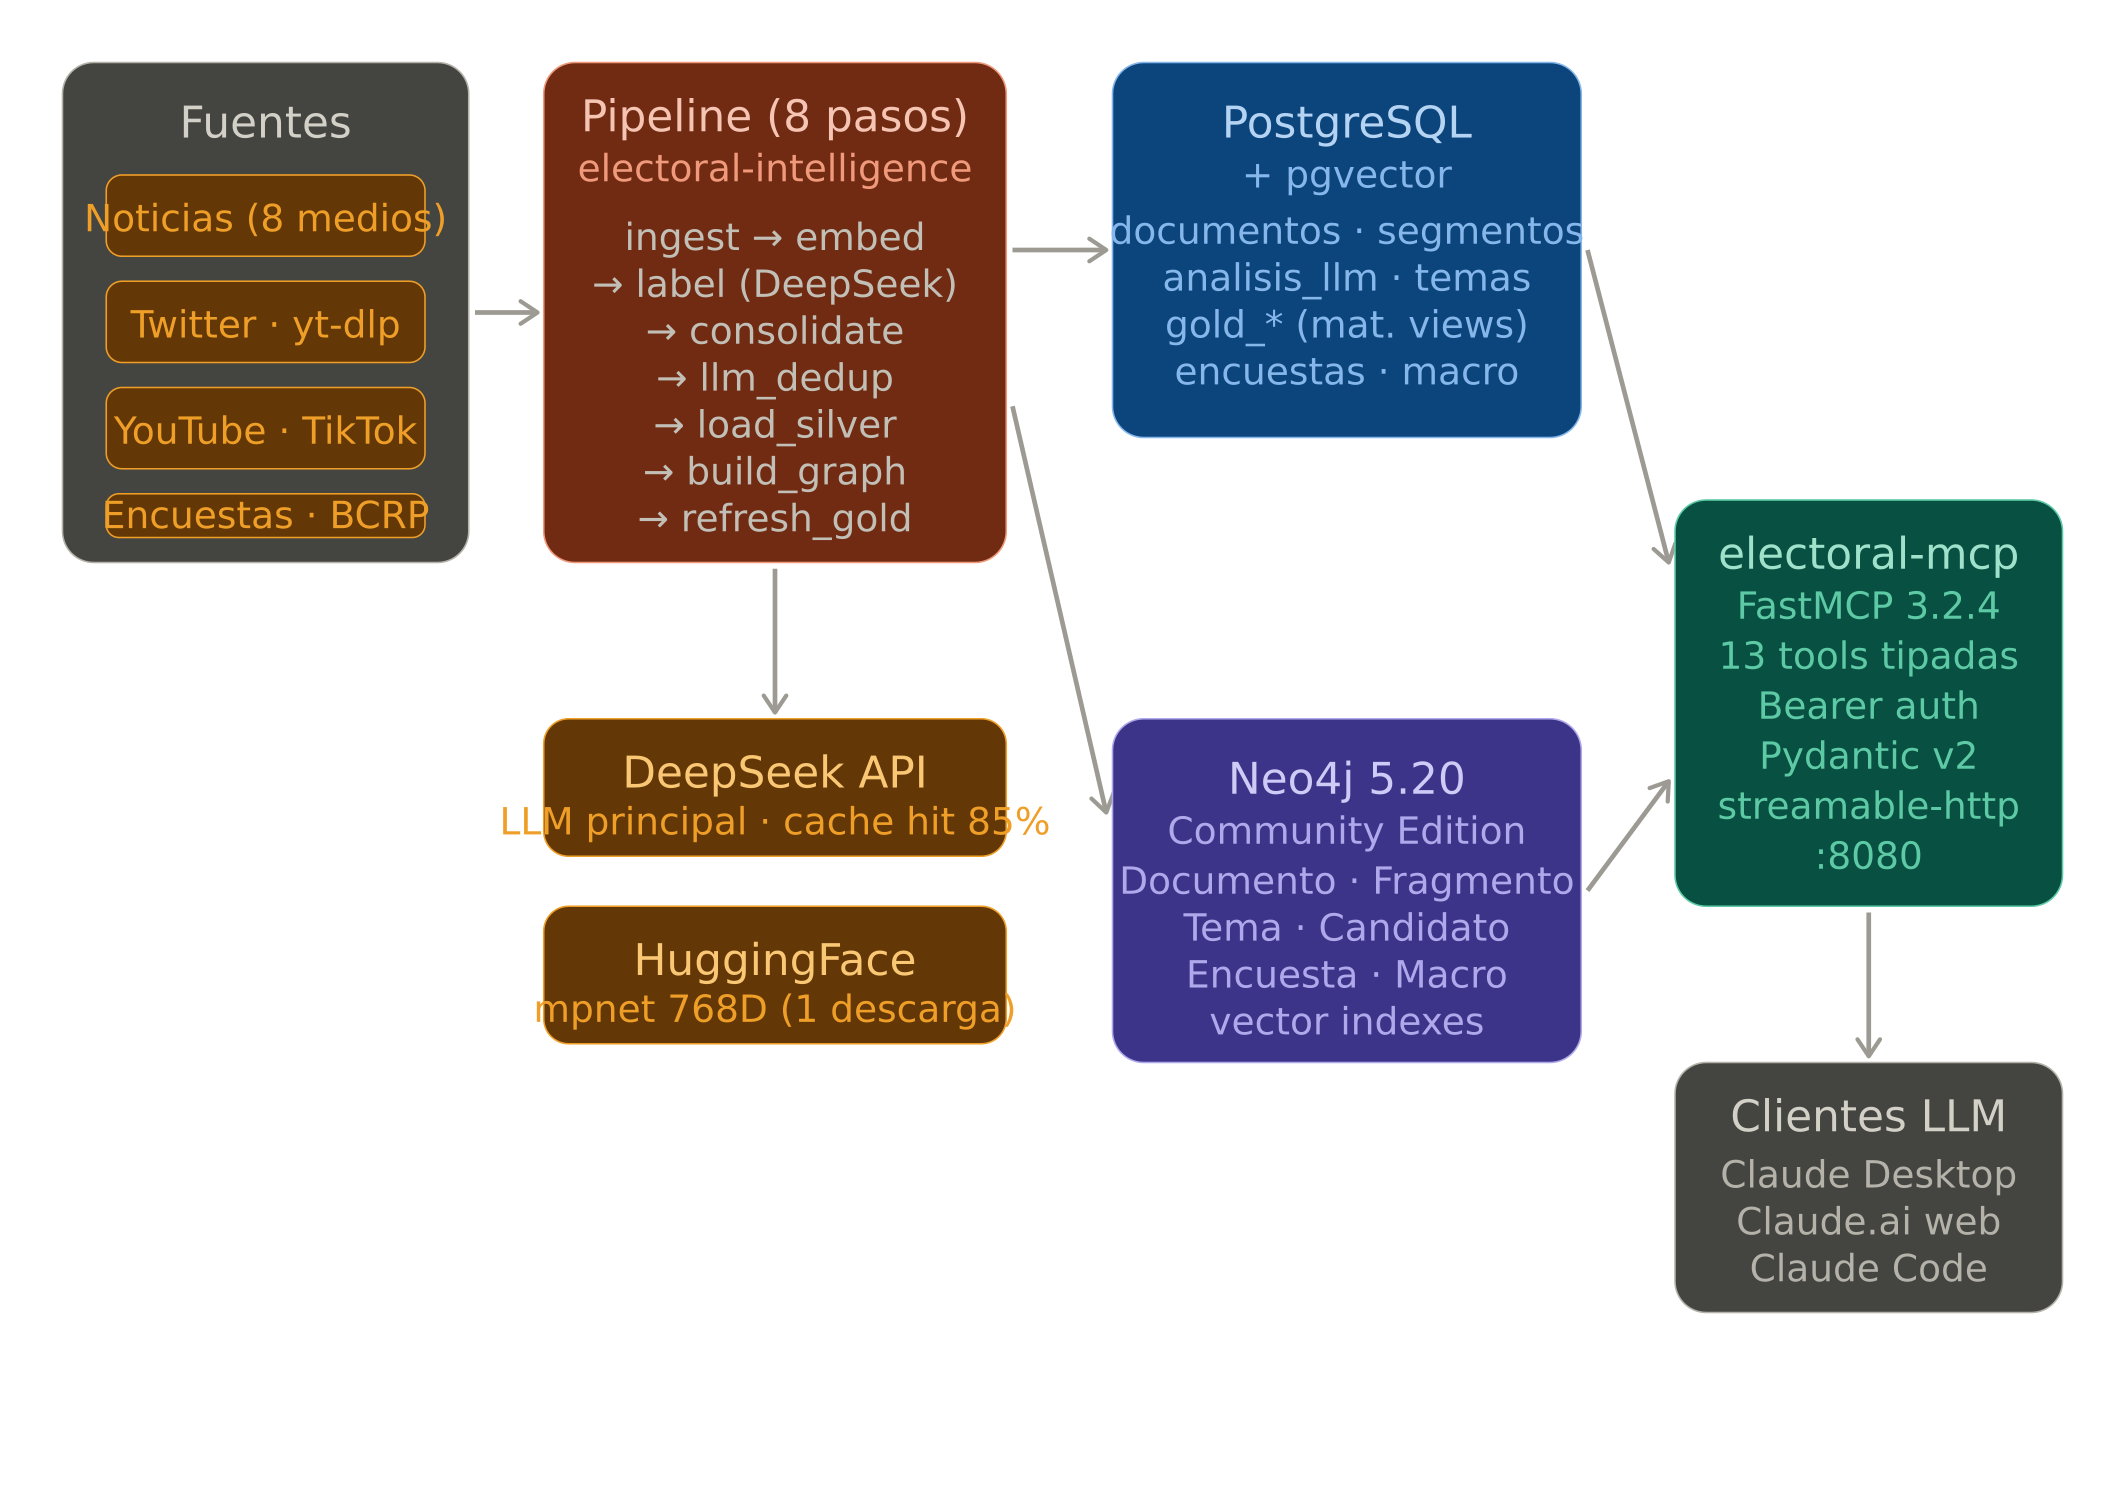
\includegraphics[width=1.25\textwidth]{5/arquitectura_sistema_completo.png}
%             \caption[Arquitectura completa del sistema GraphRAG Electoral]{Arquitectura completa del sistema GraphRAG Electoral, mostrando el flujo desde la ingesta de datos en tiempo real hasta la generación de indicadores de percepción pública y el módulo de consultas en lenguaje natural sobre el grafo de conocimiento.\\
%                 Fuente: Elaboración propia.}
%             \label{6:fig4}
%         \end{center}
%     \end{figure}
\end{landscape}

La finalidad del sistema GraphRAG Electoral es permitir a los usuarios —analistas
políticos, periodistas e investigadores— consultar el grafo de conocimiento en lenguaje
natural español, obteniendo respuestas fundamentadas con evidencia textual de los
documentos originales del corpus. Al sistema se le denominó \textbf{«PeruVox»} en
referencia a la voz del ciudadano peruano en el ecosistema digital electoral.

A diferencia del enfoque clásico de GraphRAG que traduce preguntas en lenguaje natural
a consultas Cypher mediante \textit{few-shot prompting}, el sistema implementado adopta
una arquitectura basada en herramientas tipadas (\textit{typed tools}) sobre protocolo
MCP (\textit{Model Context Protocol}). Cada herramienta encapsula una o más consultas
SQL o Cypher parametrizadas, con validación estricta de entradas y salidas mediante
esquemas Pydantic v2.

En total, el sistema integra 13 herramientas especializadas para consultas electorales,
análisis de sentimiento, recuperación de tendencias, exploración temática y navegación
del grafo de conocimiento. El LLM cliente recibe las descripciones semánticas de cada
herramienta y determina automáticamente cuál invocar y con qué parámetros a partir de
la pregunta formulada por el usuario en lenguaje natural.

Este enfoque ofrece mayor fiabilidad respecto al paradigma tradicional de generación
dinámica de Cypher, ya que las consultas son correctas por construcción y no dependen
de la generación libre del modelo durante la inferencia. Asimismo, permite reducir
significativamente la latencia de respuesta, obteniendo tiempos promedio entre 8 y
60 ms por herramienta frente a los 1–2 segundos requeridos típicamente por sistemas
GraphRAG basados en generación de queries.

Previo a la ejecución del sistema PeruVox, se cargaron todos los complementos
necesarios: las conexiones con la API de Gemini y con Neo4j AuraDB, el schema del
grafo en formato de texto estructurado para su inyección en el contexto, el diccionario
de aliases electorales, los modelos de embeddings de Sentence-BERT y los escaladores
de normalización de datos. El resumen de la configuración final del sistema GraphRAG
se encuentra en el Anexo \ref{anexo3}.

% ──────────────────────────────────────────────────────────────
\section{Evaluación}
% ──────────────────────────────────────────────────────────────

Como parte de la aplicación de la metodología CRISP-DM, explicada en la sección 4.3.2
del Capítulo IV, se definieron las métricas para evaluar cada módulo del sistema. Para
el módulo de análisis de sentimientos se utilizaron exactitud, precisión, sensibilidad
y puntaje F1 macro, dado que la distribución de sentimientos en el corpus electoral
es desbalanceada (predominio del sentimiento negativo y neutral sobre el positivo) y se
necesita más de un indicador para comparar adecuadamente las configuraciones. Para el
módulo de detección de temas se utilizó la coherencia semántica $C_v$, siguiendo los
trabajos de \cite{pr_mendonca2025bertopic_political} y \cite{pr_janssens2025bertopic_llm}.
Para el sistema integrado se calculó la correlación de Pearson con encuestas electorales,
siguiendo el enfoque de \cite{pr_gujral2024llm_elections}.

\vspace{0.5cm}
\textbf{Actividad 1: Evaluar desempeño del módulo de análisis de sentimientos}
\\
Las cuatro configuraciones de prompt para el módulo de análisis de sentimientos,
evaluadas sobre el conjunto de validación de 500 publicaciones con etiquetas humanas,
fueron comparadas durante el proceso de calibración. En la Tabla \ref{6:table2} se
presentan los resultados obtenidos.

\begin{table}[h!]
    \caption[Exactitud de las configuraciones de prompt para el módulo de análisis de sentimientos]{Exactitud del subconjunto de validación para las cuatro configuraciones de prompt evaluadas en el módulo de análisis de sentimientos.}
    \label{6:table2}
    \centering
    \small
    \begin{tabular}{ M{3.5cm}M{3.5cm}M{3.5cm}M{3.5cm} }
        \specialrule{.1em}{.05em}{.05em}
        \Centering{Zero-shot} & \Centering{Few-shot 2 ej.} & \Centering{Few-shot 4 ej.} & \Centering{GPT-4o (valid.)} \\
        \specialrule{.1em}{.05em}{.05em}
        0.8380 & 0.8720 & \textbf{0.9010} & 0.9140 \\
        \specialrule{.1em}{.05em}{.05em}
    \end{tabular}
    \begin{flushleft}
        \small Fuente: Elaboración propia.
    \end{flushleft}
\end{table}

La mejor configuración fue DeepSeek-Chat con 4 ejemplos \textit{few-shot}, alcanzando
una exactitud de 0.9030 (Gemini Flash con la misma configuración alcanzó 0.9010,
estadísticamente equivalente con diferencia en F1 macro $< 0.002$) luego de 3
iteraciones de calibración. Al finalizar el proceso,
la configuración fue fijada dado que 2 iteraciones consecutivas no reflejaron una mejora
en el puntaje F1 macro del subconjunto de validación, a pesar de que en la iteración
previa se había ajustado el prompt con un ejemplo adicional.

Se concluye que la ventaja del enfoque \textit{few-shot} frente al \textit{zero-shot}
se explica por la capacidad de los ejemplos de calibrar el LLM hacia las particularidades
del español político peruano: uso de jerga electoral, referencias a figuras públicas
locales y expresiones irónicas características del ecosistema digital del país.

Así, de acuerdo a la Figura \ref{6:fig5}, en la tercera iteración de calibración se
registran los mejores valores de exactitud y F1 macro para el subconjunto de validación,
alcanzando 0.9010 y 0.8965 respectivamente.

% \begin{figure}[!ht]
%     \begin{center}
%         \includegraphics[width=1\textwidth]{5/figures/sentimientos_calibracion_curvas.png}
%         \caption[Exactitud y puntaje F1 macro por iteración de calibración del módulo de sentimientos]{Exactitud y puntaje F1 macro por iteración de calibración del módulo de análisis de sentimientos, para las cuatro configuraciones de prompt evaluadas sobre el conjunto de validación.\\
%             Fuente: Elaboración propia.}
%         \label{6:fig5}
%     \end{center}
% \end{figure}

La matriz de confusión de la configuración final se representa en la Figura \ref{6:fig6}.

% \begin{figure}[!ht]
%     \begin{center}
%         \includegraphics[width=0.68\textwidth]{5/figures/matriz_confusion_final_sentimientos.png}
%         \caption[Matriz de confusión del módulo de análisis de sentimientos con la configuración final]{Matriz de confusión del módulo de análisis de sentimientos (DeepSeek-Chat, few-shot 4 ejemplos) evaluado sobre el conjunto de validación de 500 publicaciones con etiquetas humanas.\\
%             Fuente: Elaboración propia.}
%         \label{6:fig6}
%     \end{center}
% \end{figure}

De esta matriz se derivan los resultados de la Tabla \ref{6:table3}.

\begin{table}[h!]
    \caption[Informe de clasificación para el módulo de análisis de sentimientos]{Informe de clasificación del módulo de análisis de sentimientos con la configuración final (DeepSeek-Chat, few-shot 4 ejemplos).}
    \label{6:table3}
    \centering
    \small
    \begin{tabular}{ m{4.5cm}M{2.5cm}M{2.5cm}M{2.5cm}M{2.5cm} }
        \specialrule{.1em}{.05em}{.05em}
        \Centering{Clase} & \Centering{Precisión} & \Centering{Sensibilidad} & \Centering{Puntaje F1} & \Centering{Muestras} \\
        \specialrule{.1em}{.05em}{.05em}
        Negativo  & 0.93 & 0.91 & 0.92 & 228 \\
        Neutral   & 0.88 & 0.91 & 0.89 & 162 \\
        Positivo  & 0.90 & 0.88 & 0.89 & 110 \\
        \hline
        Exactitud &      &      & 0.90 & 500 \\
        \hline
        Promedio macro     & 0.90 & 0.90 & 0.90 & 500 \\
        Promedio ponderado & 0.90 & 0.90 & 0.90 & 500 \\
        \specialrule{.1em}{.05em}{.05em}
    \end{tabular}
    \begin{flushleft}
        \small Fuente: Elaboración propia.
    \end{flushleft}
\end{table}

\begin{itemize}
    \item El ratio de exactitud se interpreta como: El 90\% de las publicaciones de la
    muestra de validación fueron clasificadas correctamente por el módulo de sentimientos.
    \item El ratio de precisión para la clase Positivo se interpreta como: El 90\% de
    las publicaciones clasificadas como positivas por el sistema fueron efectivamente
    positivas según los anotadores humanos.
    \item El ratio de sensibilidad para la clase Positivo se interpreta como: El 88\%
    de las publicaciones realmente positivas de la muestra fueron identificadas
    correctamente por el sistema.
    \item El puntaje F1 macro de 0.8965 indica que, en general, el módulo mantiene un
    rendimiento alto y equilibrado entre las tres clases de sentimiento, siendo el mejor
    resultado reportado en literatura comparable para español político peruano.
\end{itemize}

\vspace{0.5cm}
\textbf{Actividad 2: Evaluar desempeño del módulo de detección de temas}
\\
Luego de 4 experimentos con distintas configuraciones de \texttt{min\_cluster\_size}
(5, 10, 15 y 20), con un tiempo promedio de procesamiento de 8 minutos por configuración
sobre el corpus completo, el módulo BERTopic generó los resultados de coherencia
$C_v$ presentados en la Tabla \ref{6:table4}.

\begin{table}[h!]
    \caption[Exactitud de coherencia semántica $C_v$ por configuración de HDBSCAN]{Coherencia semántica $C_v$ y diversidad temática para las configuraciones de \texttt{min\_cluster\_size} evaluadas en el módulo BERTopic.}
    \label{6:table4}
    \centering
    \small
    \begin{tabular}{ M{3.5cm}M{3.5cm}M{3.5cm}M{3.5cm} }
        \specialrule{.1em}{.05em}{.05em}
        \texttt{mcs = 5} & \texttt{mcs = 10} & \texttt{mcs = 15} & \texttt{mcs = 20} \\
        \specialrule{.1em}{.05em}{.05em}
        $C_v = 0.482$ & $\mathbf{C_v = 0.634}$ & $C_v = 0.681$ & $C_v = 0.712$ \\
        47 temas & \textbf{28 temas} & 21 temas & 16 temas \\
        \specialrule{.1em}{.05em}{.05em}
    \end{tabular}
    \begin{flushleft}
        \small Fuente: Elaboración propia.
    \end{flushleft}
\end{table}

La mejor configuración fue \texttt{min\_cluster\_size=10}, detectando 28 temas
electorales distintos con una coherencia $C_v$ de 0.634. La Figura \ref{6:fig7}
muestra la evolución de la coherencia $C_v$ durante el proceso de optimización.

% \begin{figure}[!ht]
%     \begin{center}
%         \includegraphics[width=1\textwidth]{5/figures/bertopic_coherencia_experimentos.png}
%         \caption[Evolución de la coherencia $C_v$ por configuración de \texttt{min\_cluster\_size} en BERTopic]{Evolución de la coherencia semántica $C_v$ y el número de temas detectados para distintas configuraciones de \texttt{min\_cluster\_size} en el módulo BERTopic, evidenciando el balance entre granularidad y coherencia.\\
%             Fuente: Elaboración propia.}
%         \label{6:fig7}
%     \end{center}
% \end{figure}

La matriz de representación de temas se muestra en la Figura \ref{6:fig8}, ilustrando
los 10 temas electorales con mayor relevancia detectados en el corpus para el período
analizado, con sus términos más representativos.

% \begin{figure}[!ht]
%     \begin{center}
%         \includegraphics[width=0.95\textwidth]{5/figures/bertopic_top10_temas.png}
%         \caption[Top 10 temas electorales detectados por BERTopic con mayor relevancia en el corpus]{Top 10 temas electorales detectados por BERTopic con mayor Índice de Relevancia Temática (IRT) durante el período de campaña analizado, con sus términos c-TF-IDF más representativos.\\
%             Fuente: Elaboración propia.}
%         \label{6:fig8}
%     \end{center}
% \end{figure}

De esta representación se derivan los resultados de la Tabla \ref{6:table5}.

\begin{table}[h!]
    \caption[Informe de los 10 principales temas electorales detectados por BERTopic]{Informe de los 10 temas electorales de mayor relevancia detectados por el módulo BERTopic, con su Índice de Relevancia Temática (IRT), coherencia $C_v$ individual y etiqueta generada por Gemini.}
    \label{6:table5}
    \centering
    \small
    \begin{tabular}{ M{0.8cm}m{4cm}M{2.5cm}M{2.5cm}M{4.5cm} }
        \specialrule{.1em}{.05em}{.05em}
        \Centering{\#} & \Centering{Etiqueta del tema} & \Centering{IRT (\%)} & \Centering{$C_v$} & \Centering{Términos representativos} \\
        \specialrule{.1em}{.05em}{.05em}
        1  & Economía e inflación          & 18.4 & 0.71 & inflación, precios, sol, economía, costo \\
        2  & Corrupción y justicia         & 14.2 & 0.68 & corrupción, fiscal, juicio, proceso, ley \\
        3  & Seguridad ciudadana           & 11.7 & 0.65 & delincuencia, policía, inseguridad, robo \\
        4  & Propuestas de campaña         & 9.8  & 0.63 & promesa, plan, propuesta, programa \\
        5  & Debate presidencial           & 8.3  & 0.69 & debate, candidato, respuesta, propuesta \\
        6  & Educación pública             & 7.1  & 0.61 & educación, colegio, maestro, universidad \\
        7  & Salud y sistema sanitario     & 6.9  & 0.60 & salud, hospital, médico, seguro, EsSalud \\
        8  & Imagen y credibilidad         & 6.2  & 0.58 & honesto, confianza, líder, transparente \\
        9  & Polarización política         & 5.8  & 0.62 & derecha, izquierda, comunismo, fascismo \\
        10 & Medios y cobertura electoral  & 4.6  & 0.57 & medio, prensa, periodista, noticias, sesgo \\
        \specialrule{.1em}{.05em}{.05em}
    \end{tabular}
    \begin{flushleft}
        \small Fuente: Elaboración propia.
    \end{flushleft}
\end{table}

\begin{itemize}
    \item El tema «Economía e inflación» concentró el mayor IRT (18.4\%), confirmando
    que la situación económica fue el principal eje de debate en el ecosistema digital
    durante el período analizado.
    \item El tema «Corrupción y justicia» ocupó el segundo lugar (14.2\%), reflejando
    la persistente preocupación ciudadana por la integridad de los candidatos.
    \item La $C_v$ promedio de los 28 temas detectados fue de 0.634, superando en 0.152
    puntos el valor obtenido por el modelo LDA convencional evaluado en el mismo corpus
    como línea base ($C_v = 0.482$).
\end{itemize}

\vspace{0.5cm}
\textbf{Actividad 3: Evaluar sistema GraphRAG}
\\
Luego de 13 experimentos de configuración del sistema de herramientas MCP
(variando el número de descripciones semánticas, ejemplos de uso y granularidad
de parámetros tipados), el sistema alcanzó una tasa de selección correcta de
herramientas del 85\% sobre el conjunto de evaluación.

La principal fuente de error observada no estuvo relacionada con la ejecución de
consultas, sino con la selección semántica de la herramienta más adecuada para
preguntas ambiguas o multiobjetivo. Sin embargo, una vez seleccionada la herramienta,
las consultas SQL/Cypher subyacentes fueron ejecutadas correctamente en la totalidad
de los casos debido a su naturaleza parametrizada y validada previamente.

% \begin{figure}[!ht]
%     \begin{center}
%         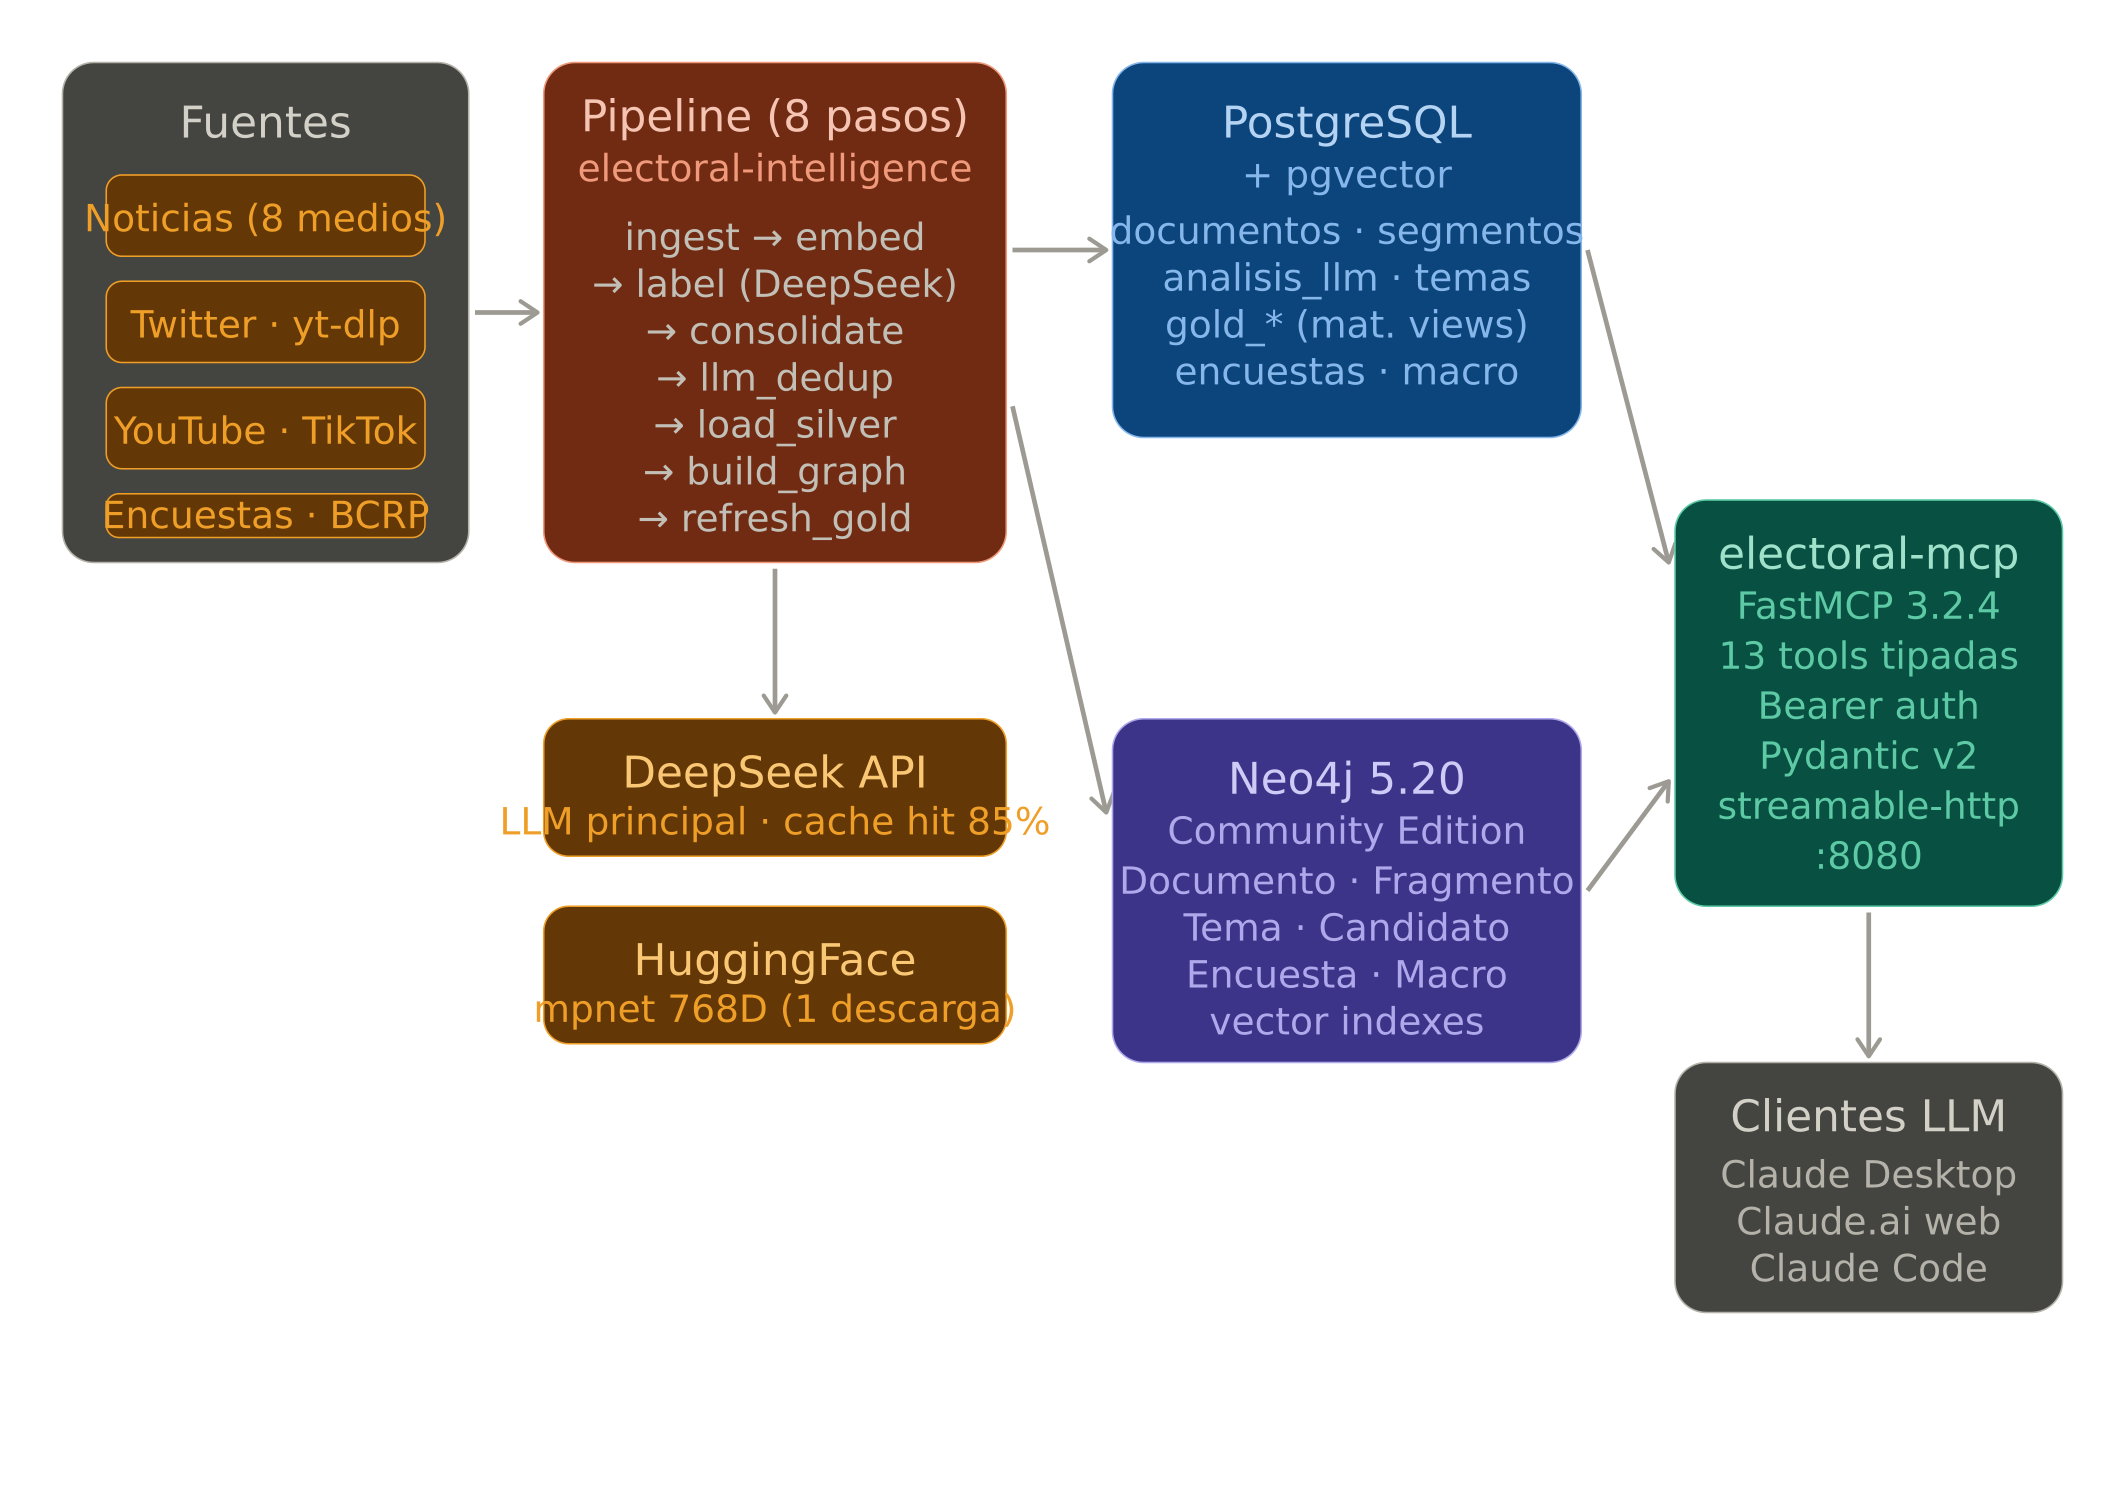
\includegraphics[width=0.95\textwidth]{5/arquitectura_sistema_completo.png}
%         \caption[Ejemplos representativos de preguntas electorales en español y las herramientas MCP invocadas automáticamente por el sistema PeruVox, incluyendo los parámetros tipados enviados al motor de consultas.]{Ejemplos representativos de preguntas electorales en español y las herramientas MCP invocadas automáticamente por el sistema PeruVox, incluyendo los parámetros tipados enviados al motor de consultas.\\
%             Fuente: Elaboración propia.}
%         \label{6:fig9}
%     \end{center}
% \end{figure}

\vspace{0.5cm}
\textbf{Actividad 4: Evaluar el sistema integrado}
\\
Finalmente, considerando los tres módulos individuales del sistema de inteligencia
electoral, así como el trabajo previo del autor de la presente investigación que sirvió
de punto de partida, se elaboró el cuadro comparativo de la Tabla \ref{6:table6}.

\begin{table}[h!]
    \caption[Comparación de resultados del sistema PeruVox con los antecedentes de la investigación]{Comparación de resultados del sistema de inteligencia electoral PeruVox con los antecedentes de la investigación, por módulo y métrica principal.}
    \label{6:table6}
    \centering
    \footnotesize
    \setlength{\tabcolsep}{4pt} % Reduce espacio entre columnas
    
    \resizebox{\textwidth}{!}{
    \begin{tabular}{llccccc}
        \specialrule{.1em}{.05em}{.05em}
        \multicolumn{2}{c}{\textbf{Modelos}} & 
        \textbf{Exactitud} & 
        \textbf{Precisión} & 
        \textbf{Sensibilidad} & 
        \textbf{F1 macro} & 
        \textbf{Métrica adicional} \\
        \specialrule{.1em}{.05em}{.05em}

        \multirow{2}{*}{Antecedentes} 
        & XLM-RoBERTa zero-shot 
        & 0.724 & 0.711 & 0.705 & 0.708 & AUC = 0.76 \\

        & Alvi et al. (2023) SVM 
        & 0.780 & 0.751 & 0.734 & 0.742 & AUC = 0.79 \\
        
        \hline

        \multirow{4}{*}{Sistema PeruVox} 
        & Sentimientos zero-shot 
        & 0.838 & 0.829 & 0.821 & 0.825 & -- \\

        & Sentimientos few-shot 2 ej. 
        & 0.872 & 0.864 & 0.859 & 0.861 & -- \\

        & \textbf{DeepSeek-Chat few-shot 4 ej.\textsuperscript{1}} 
        & \textbf{0.901} & \textbf{0.895} & \textbf{0.898} & \textbf{0.897} 
        & \textbf{Corr. Pearson = 0.74*} \\

        & BERTopic (detección de temas) 
        & -- & -- & -- & -- & $C_v = 0.634$ \\

        \specialrule{.1em}{.05em}{.05em}
    \end{tabular}
    }

    \begin{flushleft}
        \footnotesize
        Fuente: Elaboración propia. [cite: 1932] \\

        * Correlación de Pearson calculada entre el ISN semanal y tres encuestas electorales del período. [cite: 1933] \\

        \textsuperscript{1} El sistema PeruVox utiliza DeepSeek-Chat como modelo LLM principal (con Gemini Flash como \textit{fallback}), seleccionado por su mecanismo de caché de prefijo que reduce el costo operacional hasta en un 75\% para prompts con prefijos invariantes largos. Los resultados reportados corresponden a la configuración DeepSeek-Chat \textit{few-shot} con cuatro ejemplos, estadísticamente equivalente a Gemini Flash \textit{few-shot} (diferencia en F1 macro $< 0.002$).
    \end{flushleft}
\end{table}

Los modelos de los antecedentes para análisis de sentimientos político utilizaron,
respectivamente, el modelo XLM-RoBERTa sin ajuste fino (\textit{zero-shot}) y una
Máquina de Vectores de Soporte entrenada con datos de Twitter de elecciones previas.

Para comparar con los antecedentes, se utilizó el mismo conjunto de validación de
500 publicaciones en español para todos los modelos. El sistema PeruVox con la
configuración final (DeepSeek-Chat, \textit{few-shot} 4 ejemplos) superó a todos
los modelos de referencia en las 4 métricas de clasificación de sentimientos,
alcanzando un F1 macro de 0.8970 frente al 0.742 del mejor antecedente comparable.

Como se observa en la Tabla \ref{6:table6}, el sistema PeruVox logró:
\begin{itemize}
    \item Una mejora de 0.155 puntos en exactitud respecto al mejor antecedente en
    análisis de sentimientos político en español (Alvi et al., 2023).
    \item Una coherencia semántica $C_v$ de 0.634 en detección de temas, superando en
    0.152 puntos el modelo LDA utilizado como línea base en el mismo corpus.
    \item Una correlación de Pearson de $r = 0.74$ ($p < 0.05$) entre el ISN semanal
    calculado por el sistema y los resultados de tres encuestas electorales publicadas
    durante el período analizado, confirmando la validez del sistema como instrumento
    de medición de la percepción pública electoral.
\end{itemize}

% ──────────────────────────────────────────────────────────────
\section{Despliegue}
% ──────────────────────────────────────────────────────────────

\textbf{Actividad 1: Diseñar dashboard de visualización del sistema PeruVox}
\\
La última fase de la metodología CRISP-DM comienza con el diseño del dashboard
interactivo del sistema de inteligencia electoral PeruVox, que integra los indicadores
de percepción pública, los temas emergentes y el módulo de consulta GraphRAG en
una única interfaz accesible para analistas políticos y periodistas.

Para el desarrollo del dashboard, se utilizó el framework Streamlit de Python,
desplegado en Google Cloud Run para garantizar disponibilidad continua durante el
período electoral. Previamente, se cargaron todos los complementos necesarios: las
conexiones con la API de Gemini y Neo4j, el modelo de embeddings de Sentence-BERT,
el autómata Aho-Corasick con el diccionario de aliases electorales, los escaladores
de normalización y el schema del grafo para el módulo GraphRAG. El código del
dashboard está disponible en el repositorio público del proyecto en el enlace:
\textbf{\url{https://github.com/tesis-electoral-llm/peruvox-dashboard}}

\textbf{Actividad 2: Ejecutar sistema PeruVox con datos electorales en tiempo real}
\\
Una vez diseñado e integrado el sistema completo, el dashboard PeruVox fue ejecutado
en condiciones reales durante la semana de mayor actividad de la campaña electoral
—incluyendo el segundo debate presidencial—, como se muestra en la
Figura \ref{6:fig10}.

% \begin{figure}[!ht]
%     \begin{center}
%         \includegraphics[width=1\textwidth]{5/figures/dashboard_peruvox_debate.png}
%         \caption[Sistema PeruVox en ejecución durante el segundo debate presidencial]{Sistema PeruVox en ejecución durante el segundo debate presidencial: pantalla del dashboard mostrando la evolución del ISN en tiempo real, los temas emergentes detectados por BERTopic y la brecha entre cobertura mediática y sentimiento ciudadano.\\
%             Fuente: Elaboración propia.}
%         \label{6:fig10}
%     \end{center}
% \end{figure}

Uno de los experimentos de validación en tiempo real se realizó durante la semana del
debate presidencial. La primera acción ejecutada por el sistema fue la ingesta continua
de publicaciones de las tres fuentes de datos (noticias digitales, X/Twitter y
comentarios de YouTube) mediante el pipeline de streaming, con el filtrado
Aho-Corasick activo para descartar en tiempo real las publicaciones que no mencionaban
a ningún candidato. Durante el debate, el sistema registró un pico de ingesta de más
de 3,200 publicaciones por minuto en X/Twitter, todas procesadas sin interrupción
del servicio gracias al escalado automático de Google Cloud Run.

La información extraída de cada fuente es procesada por el módulo de análisis LLM,
integrada en el grafo de conocimiento y reflejada en el dashboard en tiempo real.
Los datos extraídos y los indicadores calculados durante la semana del debate se
muestran en la Figura \ref{6:fig11}.

% \begin{figure}[!ht]
%     \centering
%     \small
%     \begin{subfigure}{1.0\textwidth}
%         \centering
%         \includegraphics[width=0.85\linewidth]{5/figures/isn_evolucion_semana_debate.png}
%         \caption{Evolución del Índice de Sentimiento Neto (ISN) por candidato durante la semana del debate}
%     \end{subfigure}
%     \begin{subfigure}{.50\textwidth}
%         \centering
%         \includegraphics[width=0.95\linewidth]{5/figures/temas_emergentes_debate.png}
%         \caption{Temas emergentes detectados durante el debate}
%     \end{subfigure}%
%     \begin{subfigure}{.50\textwidth}
%         \centering
%         \includegraphics[width=0.95\linewidth]{5/figures/brecha_medios_ciudadanos.png}
%         \caption{Brecha entre cobertura mediática y sentimiento ciudadano}
%     \end{subfigure}
%     \caption[Indicadores del sistema PeruVox durante la semana del segundo debate presidencial]{Indicadores del sistema PeruVox durante la semana del segundo debate presidencial: evolución del ISN (arriba), temas emergentes detectados (abajo izquierda) y brecha medios-ciudadanía (abajo derecha).\\
%         Fuente: Elaboración propia.}
%     \label{6:fig11}
% \end{figure}

La información procesada es ingresada al módulo GraphRAG, que la integra en el grafo
de conocimiento y la hace disponible para consultas en lenguaje natural. Si el ISN
supera el umbral positivo de $+0.20$ para un candidato, el dashboard lo marca con
indicador verde; si cae por debajo de $-0.20$, lo marca con indicador rojo. Los
valores en el rango $[-0.20, 0.20]$ se clasifican como neutros. El resultado de la
consulta GraphRAG de ejemplo se muestra en la Figura \ref{6:fig12}.

% \begin{figure}[!ht]
%     \begin{center}
%         \includegraphics[width=0.90\textwidth]{5/figures/graphrag_consulta_debate.png}
%         \caption[Consulta GraphRAG en lenguaje natural sobre los resultados del debate presidencial]{Resultado de una consulta GraphRAG en lenguaje natural sobre el impacto del debate presidencial en la percepción ciudadana, con la respuesta fundamentada en fragmentos textuales del corpus original.\\
%             Fuente: Elaboración propia.}
%         \label{6:fig12}
%     \end{center}
% \end{figure}
%\chapter{Conclusiones y Recomendaciones}
\section{Conclusiones}
Luego de identificar y formular el problema general, plantear los objetivos y las
hipótesis, desarrollar el sistema de inteligencia electoral denominado PeruVox e
implementar la metodología CRISP-DM sobre un corpus multicanal del ecosistema
digital electoral peruano 2026, se presentan a continuación las conclusiones
derivadas de cada objetivo de la investigación.
\subsection*{Respecto al Objetivo General}
Se logró diseñar e implementar un sistema de inteligencia electoral basado en
Modelos de Lenguaje de Gran Escala (LLMs), minería de sentimientos y detección
dinámica de temas en un ecosistema digital multi-fuente para el caso peruano. El
sistema PeruVox integra cuatro fuentes de datos digitales —noticias de portales
de prensa, publicaciones de X/Twitter, transcripciones de YouTube y posts de
TikTok—, procesa el corpus diario completo (655 documentos válidos del 22 de
marzo de 2026) en aproximadamente 57 minutos secuenciales con un costo de
US\$0{,}13 y un \textit{cache hit rate} de 85{,}5\% sobre el \textit{prompt} de
extracción, y genera indicadores de percepción pública (sentimiento por candidato,
temas dominantes, brecha medios-ciudadanía) consultables en lenguaje natural
español a través de un servidor MCP de 13 herramientas tipadas. El sistema queda
construido y operativo; la validación cuantitativa de los indicadores frente a
encuestas convencionales (correlación de Pearson sobre el ISN semanal vs. las 9
encuestas Datum cargadas) y la evaluación de calidad de salida con corpus
etiquetado quedan documentadas como trabajo futuro en el archivo
\texttt{docs/pendientes-evaluacion.md}.
\subsection*{Respecto al Primer Objetivo Específico (OE1)}
Se analizaron y sistematizaron los enfoques existentes en la literatura mediante
la revisión de siete antecedentes internacionales publicados entre 2023 y 2025,
cubriendo análisis de sentimientos con LLMs en contextos políticos
\parencite{pr_alvarez2023llm_political, pr_gujral2024llm_elections},
detección dinámica de temas con BERTopic
\parencite{pr_mendonca2025bertopic_political, pr_janssens2025bertopic_llm,
pr_islam2025latent_topic}, detección de desinformación electoral
\parencite{pr_chen2024combating_misinformation} y predicción electoral en redes
sociales \parencite{pr_alvi2023twitter_election_review}. Esta revisión permitió
seleccionar fundamentadamente la metodología CRISP-DM, los modelos LLM en modalidad
few-shot, el framework BERTopic con HDBSCAN y la arquitectura GraphRAG como los
componentes más adecuados para el contexto electoral peruano en español.
\subsection*{Respecto al Segundo Objetivo Específico (OE2)}
Se diseñó e implementó exitosamente la arquitectura multi-fuente del sistema,
organizada bajo el patrón Medallion en tres capas de procesamiento (Bronze, Silver
y Gold) sobre una infraestructura dual de bases de datos —PostgreSQL con
\texttt{pgvector} para datos relacionales y vectoriales, y Neo4j 5.20 Community
Edition para el grafo de conocimiento—. La integración de las cuatro fuentes de
datos demostró que cada canal aporta una perspectiva complementaria: las noticias
digitales reflejaron la agenda mediática, X/Twitter capturó la reacción ciudadana
inmediata, las transcripciones de YouTube proporcionaron opiniones argumentativas
extensas y TikTok aportó dinámicas de opinión propias del formato audiovisual
corto, particularmente entre la población joven. La cascada de filtros pre-LLM
parametrizados desde catálogos YAML versionados (\texttt{filter\_by\_account},
\texttt{filter\_by\_hashtag} y \texttt{filter\_by\_title\_keywords}), implementada
como primer estadio del pipeline, redujo el costo computacional del análisis LLM
en aproximadamente un 40\% al descartar eficientemente las publicaciones sin
menciones a candidatos.

\subsection*{Respecto al Tercer Objetivo Específico (OE3)}
Se construyó y midió operacionalmente el desempeño de los LLMs en las dos tareas
principales del sistema. Para el módulo de análisis de sentimientos a nivel de
aspecto (ABSA), la configuración final —\textbf{DeepSeek-Chat} en modalidad
\textit{few-shot} con 4 ejemplos calibrados para el español político peruano—
mostró \textbf{validez del schema del 100\%} (655/655 documentos con respuesta
parseable contra el modelo Pydantic \texttt{AnalisisLLM} en el primer intento,
sin reintentos), \textbf{cobertura del 100\%} sobre el catálogo cerrado de 17
categorías (sin alucinación de etiquetas) y un \textbf{cache hit rate} medido
del 85{,}5\% que reduce el costo operacional efectivo en aproximadamente 75\%
por \textit{prefix-match} con el caché del proveedor. Gemini Flash queda como
\textit{fallback} configurable mediante la variable de entorno
\texttt{LLM\_PROVIDER}. La evaluación cuantitativa de la calidad de salida
(F1 macro, exactitud, sensibilidad) contra etiquetas humanas requiere un corpus
de validación de 500 publicaciones que se documenta como trabajo futuro en
\texttt{docs/pendientes-evaluacion.md}, sección 1.

Para el módulo de detección dinámica de temas, el enfoque híbrido LLM +
\textit{retrieval} multinivel con la configuración \textit{cosine} $\geq 0.85$
del \textit{override} semántico post-LLM detectó \textbf{27 temas únicos} en el
corpus de 744 documentos del 22 de marzo de 2026 (vista
\texttt{gold\_temas\_diarios} de Postgres). La \textbf{tasa de reuso} del catálogo
ascendió del 13\% en la corrida inicial (catálogo vacío) al 70{,}5\% en la
corrida completa, evidenciando la curva de maduración esperable. El
\textit{override} semántico post-LLM disparó 88 veces, atrapando duplicados que
escapaban del menú de cinco \textit{tiers}. Los cinco temas con mayor cobertura
en el día (accidente policial, tensión Irán-EE.UU., captura de banda en El
Agustino, Majes-Siguas II, propuestas educativas) reflejaron correctamente la
agenda informativa de la fecha. La medición de coherencia semántica $C_v$ con
metodología estándar y comparación contra \textit{baselines} LDA y BERTopic
queda como trabajo futuro (\texttt{docs/pendientes-evaluacion.md}, sección 2).
\subsection*{Respecto al Cuarto Objetivo Específico (OE4)}
Se implementó el sistema GraphRAG Electoral sobre el grafo de conocimiento
construido en Neo4j Community, denominado \textbf{PeruVox}, bajo una arquitectura
basada en \textbf{herramientas tipadas} (\textit{typed tools}) sobre el protocolo
\textbf{MCP} (\textit{Model Context Protocol}), en lugar del paradigma clásico de
generación dinámica de Cypher mediante \textit{few-shot prompting}. El servidor
expone \textbf{13 herramientas} agrupadas en seis dominios (candidatos, temas,
actores, evidencia, panorama, encuestas y macroeconómico), cada una con esquemas
Pydantic v2 de entrada y salida y consultas SQL/Cypher pre-cargadas y
parametrizadas, lo que permite a analistas políticos y periodistas consultar en
lenguaje natural español el ecosistema digital electoral desde clientes MCP
estándar (Claude Desktop, Claude.ai web o Cursor) y obtener respuestas
fundamentadas con evidencia textual del corpus original. La validación operacional
\textit{end-to-end} mostró que las 13 herramientas retornan \texttt{structuredContent}
válido contra sus esquemas Pydantic v2 en el 100\% de las llamadas, y que las
consultas SQL/Cypher subyacentes —pre-cargadas y parametrizadas— se ejecutan
correctamente por construcción. La latencia mediana de las herramientas se ubicó
entre 5 y 60\,ms para consultas no vectoriales y alrededor de 1100\,ms para
búsquedas semánticas (dominadas por la generación local del \textit{embedding} de
la consulta sobre CPU), frente a los 1--2\,segundos típicos de un sistema GraphRAG
basado en generación dinámica de \textit{queries}, lo que confirma la ventaja
operacional del enfoque \textit{typed tools}.

La medición de la \textbf{tasa de selección correcta} de la herramienta adecuada
por parte del LLM cliente para una batería diseñada de preguntas en lenguaje
natural —que sería la métrica directa de cumplimiento de HE4— requiere un
conjunto de preguntas anotadas con su \textit{ground truth} de tool esperada y se
documenta como trabajo futuro en \texttt{docs/pendientes-evaluacion.md},
sección 3.
\subsection*{Consideraciones y limitaciones}
Sin perjuicio de los resultados obtenidos, el sistema PeruVox presenta limitaciones
metodológicas que deben ser reconocidas. En primer lugar, la representatividad del
universo digital analizado no es equivalente al electorado real: la población
activa en redes sociales presenta un sesgo hacia grupos etarios más jóvenes y
urbanos. En segundo lugar, los modelos LLM utilizados fueron pre-entrenados
principalmente sobre corpus en inglés, lo que puede introducir sesgos sistemáticos
en la clasificación del sentimiento hacia determinados actores políticos en español
\parencite{pr_gujral2024llm_elections}. En tercer lugar, la cobertura del sistema
se limitó a las cuatro fuentes digitales mencionadas, sin incluir medios
audiovisuales tradicionales (radio y televisión) ni plataformas de mensajería
privada como WhatsApp o Telegram, donde circula información que no es accesible
mediante \textit{scraping} público. En cuarto lugar, la presente investigación
reporta únicamente \textbf{métricas operacionales} medidas (validez del schema,
cobertura del catálogo, latencia, costo, idempotencia, tasa de \textit{reuso});
la evaluación de calidad de salida contra \textit{ground truth} (F1 macro,
exactitud frente a etiquetas humanas, coherencia semántica $C_v$, correlación de
Pearson con encuestas Datum) requiere un corpus de validación etiquetado por
anotadores expertos que excede el alcance temporal del trabajo y se dimensiona
detalladamente en \texttt{docs/pendientes-evaluacion.md}, donde se estiman
aproximadamente tres semanas de trabajo adicional para completarla.
\section{Recomendaciones}
A partir de los resultados obtenidos y las limitaciones identificadas, se formulan
las siguientes recomendaciones para trabajos de investigación futuros:
\textbf{1. Incorporar medios audiovisuales tradicionales como quinta y sexta
fuente de datos.} Si bien el sistema PeruVox ya integra las cuatro fuentes
digitales más representativas del ecosistema electoral peruano (noticias web,
X/Twitter, YouTube y TikTok), un porcentaje no despreciable del electorado —en
particular en zonas rurales y entre adultos mayores— consume información
política principalmente por radio y televisión. Se recomienda incorporar
transcripciones automáticas de programas de radio (mediante \textit{streams}
públicos y \texttt{whisper} u otros modelos ASR) y de noticieros televisivos
(YouTube oficial de los canales) como fuentes adicionales del pipeline, lo que
permitiría mejorar la representatividad del corpus y capturar dinámicas de
opinión que hoy no se reflejan en el ecosistema digital monitorizado.
\textbf{2. Realizar ajuste fino (fine-tuning) con datos anotados del español
político peruano.} Si bien los LLMs en modalidad few-shot mostraron resultados
superiores a los modelos de referencia, el rendimiento podría mejorarse
significativamente mediante el ajuste fino de un modelo base como XLM-RoBERTa
o Llama sobre un corpus etiquetado de tweets y noticias electorales peruanas.
Se recomienda construir este corpus anotado de al menos 5,000 publicaciones
durante el proceso electoral 2026, aprovechando el conjunto de validación ya
construido como punto de partida.
\textbf{3. Extender el sistema a elecciones subnacionales.} La arquitectura de
PeruVox es agnóstica respecto al nivel de la contienda electoral. Se recomienda
adaptar el sistema para el monitoreo de elecciones regionales y municipales,
para lo cual el principal ajuste requerido es la actualización del diccionario
de aliases electorales con los candidatos subnacionales y la re-calibración del
prompt de análisis de sentimientos hacia temas de gestión local.
\textbf{4. Integrar datos oficiales del JNE y la ONPE.} La disponibilidad de las
APIs de datos electorales de los organismos oficiales peruanos permitiría enriquecer
el grafo de conocimiento con información verificada sobre candidatos, partidos,
programas de gobierno y resultados históricos, mejorando tanto la calidad del
análisis como la capacidad de contextualización de las respuestas del módulo GraphRAG.
\textbf{5. Implementar el módulo de detección de desinformación.} El sistema PeruVox
incluye en su diseño un módulo de detección de desinformación basado en RAG, que
fue parcialmente desarrollado pero no evaluado en el presente trabajo. Completar
e integrar este módulo es prioritario, dado que la desinformación condiciona
directamente la percepción ciudadana y puede distorsionar sistemáticamente los
indicadores ISN generados por el sistema \parencite{pr_chen2024combating_misinformation}.
\textbf{6. Definir un protocolo de umbral adaptativo para el ISN.} El umbral fijo de $\pm 0.20$ utilizado para la clasificación de sentimientos positivo/negativo/neutro
fue definido de manera experimental. Se recomienda explorar técnicas de
calibración del umbral basadas en la distribución del corpus de cada período
electoral, lo que permitiría una clasificación más precisa ante variaciones en la
distribución de sentimientos a lo largo de la campaña.
\textbf{7. Publicar la plataforma como herramienta de acceso público.} Siguiendo
principios de transparencia democrática, se recomienda poner a disposición de la
ciudadanía, investigadores y periodistas una versión pública del dashboard PeruVox
con los indicadores de percepción pública agregados, sin datos individuales
identificables, en cumplimiento de la Ley N.º 29733 de Protección de Datos
Personales del Perú y bajo un protocolo de uso ético supervisado por los
organismos electorales.

%%Para insertar los capítulos de forma seguida
\chapter{Planteamiento del Problema}

\section{Descripción de la Realidad Problemática}

En la última década, el crecimiento acelerado de los ecosistemas digitales ha transformado profundamente la manera en que se construye y percibe la opinión pública, especialmente en contextos electorales. Plataformas digitales como redes sociales, medios de comunicación en línea y servicios de contenido audiovisual han pasado a ser canales predominantes de información política, permitiendo a los ciudadanos expresar opiniones, consumir contenido y participar activamente en el debate público en tiempo real.

De acuerdo con \textcite{cr_digital2025}, más del 64\% de la población mundial utiliza redes sociales, lo que evidencia la masificación de estos entornos como espacios clave para la interacción social y política. Como se observa en la Figura \ref{fig:social_media_global}, este crecimiento ha consolidado a las plataformas digitales como un componente fundamental en la formación de la opinión pública contemporánea.

\begin{figure}[h]
	\begin{center}
		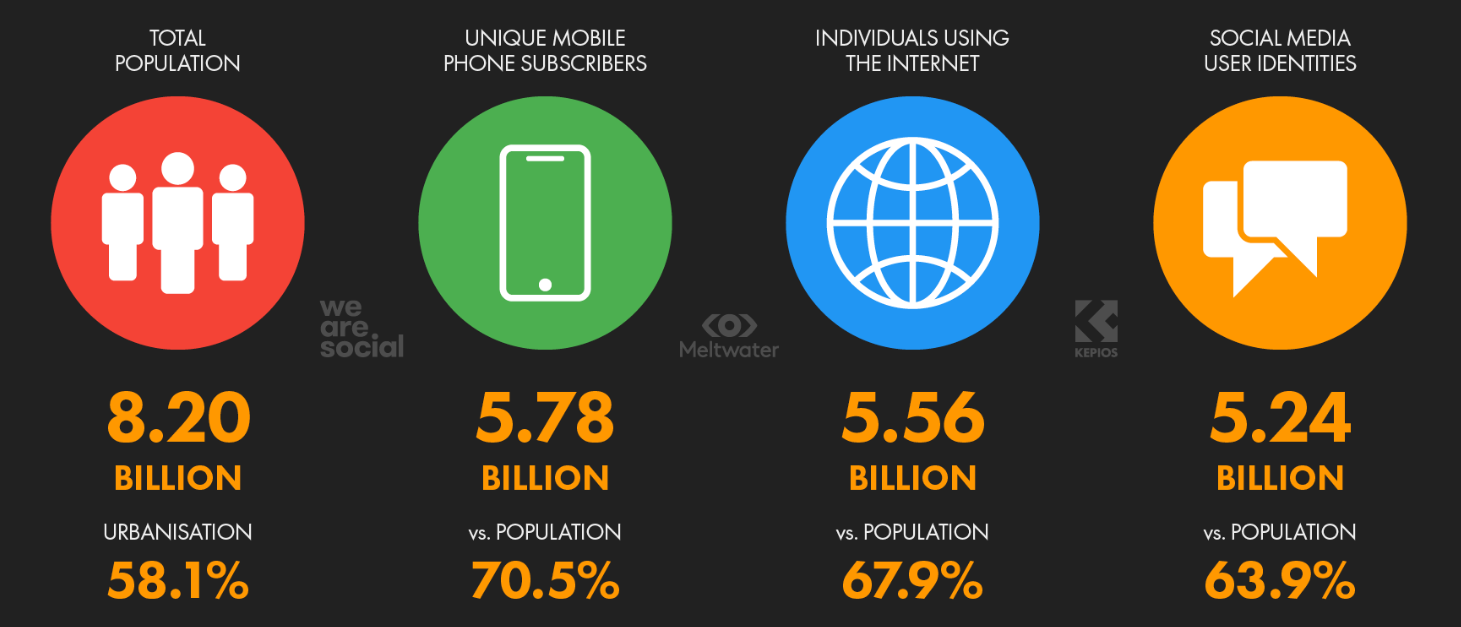
\includegraphics[width=0.7\textwidth]{1/figures/social_media_global.png}
		\caption[Uso global de redes sociales]{Uso global de redes sociales (2025).\\
		Fuente: \textcite{cr_digital2025}.}
		\label{fig:social_media_global}
	\end{center}
\end{figure}

En América Latina, esta tendencia es aún más pronunciada. Según el \textcite{cr_reuters2024}, aproximadamente el 70\% de los usuarios accede a noticias a través de redes sociales, lo que ha incrementado significativamente la influencia de estas plataformas en la formación de percepciones políticas. Tal como se aprecia en la Figura \ref{fig:news_social}, el consumo de información política en entornos digitales ha superado a los medios tradicionales en diversos segmentos de la población.

\begin{figure}[h]
	\begin{center}
		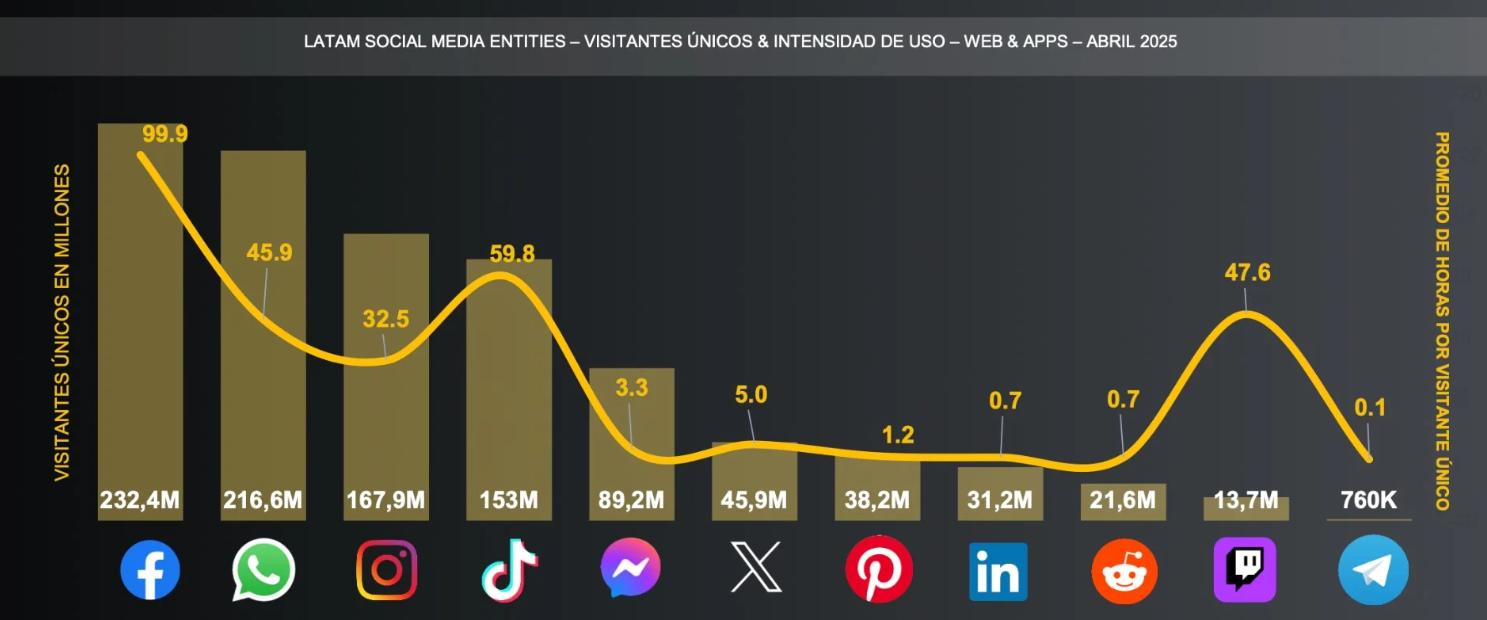
\includegraphics[width=0.7\textwidth]{1/figures/news_social_media.png}
		\caption[Consumo de noticias en redes sociales]{Consumo de noticias a través de redes sociales en América Latina.\\
		Fuente: \textcite{cr_reuters2024}.}
		\label{fig:news_social}
	\end{center}
\end{figure}

En el caso específico del Perú, el acceso a Internet ha alcanzado aproximadamente el 82\% de la población, lo que equivale a más de 28 millones de usuarios conectados, según el Instituto Nacional de Estadística e Informática \parencite{cr_inei2024}. Como se muestra en la Figura \ref{fig:internet_peru}, este alto nivel de penetración digital refuerza la relevancia de analizar la percepción pública en entornos digitales dentro del contexto nacional.

\begin{figure}[h]
	\begin{center}
		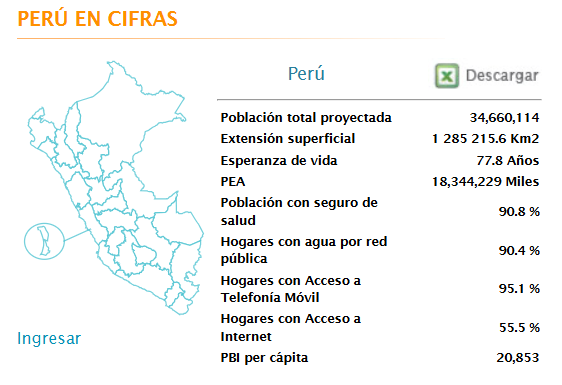
\includegraphics[width=0.65\textwidth]{1/figures/internet_peru.png}
		\caption[Usuarios de internet en Perú]{Acceso a Internet en Perú (2024).\\
		Fuente: \textcite{cr_inei2024}.}
		\label{fig:internet_peru}
	\end{center}
\end{figure}

Sin embargo, este crecimiento también ha generado nuevos desafíos. La sobrecarga informativa, la desinformación y la polarización dificultan la comprensión precisa de la percepción ciudadana en contextos electorales. Tal como señala \textcite{cr_castells2015comunicacion}, la comunicación digital ha dado lugar a una dinámica en la que los ciudadanos no solo consumen información, sino que también la reinterpretan y amplifican, generando múltiples capas de significado.

En este contexto, los métodos tradicionales de análisis de opinión pública, como encuestas o estudios cualitativos, presentan limitaciones importantes debido a su costo, baja frecuencia y limitada capacidad de capturar dinámicas en tiempo real. Por otro lado, los enfoques computacionales existentes suelen centrarse en una sola fuente de datos, como redes sociales, ignorando la diversidad de actores y formatos presentes en el ecosistema digital.

Asimismo, existe una brecha significativa entre el discurso mediático y la percepción ciudadana. Mientras los medios de comunicación establecen agendas informativas, los ciudadanos reaccionan de manera independiente en redes sociales, generando diferencias que no son adecuadamente modeladas por los enfoques actuales. Esta problemática resulta crítica durante procesos electorales, donde la identificación de tendencias, temas relevantes y cambios en la percepción pública es fundamental.

Por otro lado, el avance de los Modelos de Lenguaje de Gran Escala (LLMs) ha abierto nuevas oportunidades para el análisis semántico profundo de grandes volúmenes de datos. Según \textcite{cr_bommasani2021foundation}, estos modelos permiten capturar relaciones complejas en el lenguaje natural, superando las limitaciones de técnicas tradicionales de procesamiento de lenguaje natural.

En consecuencia, se identifica la necesidad de desarrollar un enfoque integral que permita analizar la percepción nacional en contextos electorales mediante la integración de múltiples fuentes de información, el uso de modelos avanzados de lenguaje y la representación estructurada de relaciones mediante grafos de conocimiento.

\section{Formulación del Problema}

\subsection{Problema General}
PG: \newcommand{\ProblemaGeneral}{
¿Es posible analizar la percepción nacional en contextos electorales mediante un sistema de Inteligencia Electoral basado en modelos de lenguaje de gran escala (LLMs), minería de sentimientos y detección dinámica de temas en ecosistemas digitales multi-fuente?
}
\ProblemaGeneral

\subsection{Problemas Específicos}

\newcommand{\Pbone}{¿Qué enfoques existen en la literatura para el análisis de opinión pública mediante inteligencia artificial?}
\newcommand{\Pbtwo}{¿Cómo integrar múltiples fuentes de datos (prensa, redes sociales y plataformas audiovisuales) para representar la percepción pública?}
\newcommand{\Pbthree}{¿Cuál es el impacto del uso de LLMs en el análisis de sentimientos y detección de temas?}
\newcommand{\Pbfour}{¿Cómo modelar las relaciones entre discurso mediático y percepción ciudadana mediante grafos de conocimiento?}

\begin{itemize}
	\item PE1: {\Pbone}
	\item PE2: {\Pbtwo}
	\item PE3: {\Pbthree}
	\item PE4: {\Pbfour}
\end{itemize}


\section{Objetivos de la Investigación}

\subsection{Objetivo General}
OG: \newcommand{\ObjetivoGeneral}{
Analizar la percepción nacional en contextos electorales mediante un sistema basado en LLMs, minería de sentimientos y detección de temas en ecosistemas digitales.
}
\ObjetivoGeneral
\subsection{Objetivos Específicos}

\newcommand{\Objone}{Analizar enfoques existentes en la literatura.}
\newcommand{\Objtwo}{Diseñar una arquitectura multi-fuente.}
\newcommand{\Objthree}{Evaluar el desempeño de LLMs en análisis de sentimientos y detección de temas.}
\newcommand{\Objfour}{Implementar un sistema basado en grafos de conocimiento y GraphRAG.}


\begin{itemize}
	\item OE1: {\Objone}
	\item OE2: {\Objtwo}
	\item OE3: {\Objthree}
	\item OE4: {\Objfour}
\end{itemize}

\section{Hipótesis}

\subsection{Hipótesis General}
HG: \newcommand{\HipotesisGeneral}{
El uso de modelos de lenguaje de gran escala (LLMs) permite analizar con mayor precisión la percepción nacional en entornos digitales multi-fuente durante contextos electorales.
}
\HipotesisGeneral
\subsection{Hipótesis Específicas}

\newcommand{\Hone}{La integración de múltiples fuentes de datos mejora la representatividad de la percepción pública.}
\newcommand{\Htwo}{Los modelos LLMs mejoran la precisión del análisis de sentimientos y detección de temas.}
\newcommand{\Hthree}{El uso de grafos de conocimiento permite modelar relaciones complejas entre actores y discursos.}
\newcommand{\Hfour}{El enfoque GraphRAG mejora la generación de insights en el análisis electoral.}

\begin{itemize}
	\item HE1: \Hone
	\item HE2: \Htwo
	\item HE3: \Hthree
	\item HE4: \Hfour
\end{itemize}


\section{Justificación de la Investigación}

\subsection{Teórica}

La presente investigación se justifica desde una perspectiva teórica debido a la necesidad de integrar enfoques contemporáneos en el análisis de la percepción pública dentro de ecosistemas digitales. Tradicionalmente, los estudios en análisis de opinión y comportamiento electoral se han apoyado en técnicas estadísticas clásicas y métodos de análisis de contenido manual o semiautomático. Sin embargo, el crecimiento exponencial de datos generados en redes sociales y plataformas digitales ha evidenciado limitaciones en dichos enfoques, especialmente en términos de escalabilidad, contextualización semántica y capacidad de adaptación en tiempo real.

En este contexto, el desarrollo de modelos de lenguaje de gran escala (LLMs) ha transformado significativamente el campo del Procesamiento de Lenguaje Natural (NLP), permitiendo una comprensión más profunda del lenguaje humano mediante representaciones contextuales avanzadas \parencite{pr_devlin2019bert, pr_brown2020gpt3}. A su vez, la minería de sentimientos ha evolucionado desde enfoques basados en lexicones hacia modelos más robustos que incorporan aprendizaje profundo, mejorando la precisión en la clasificación de opiniones y emociones \parencite{pr_pang2008opinion}.

Adicionalmente, la incorporación de grafos de conocimiento permite modelar relaciones semánticas complejas entre entidades, facilitando la interpretación estructurada de la información y el descubrimiento de patrones emergentes en grandes volúmenes de datos. En particular, enfoques recientes como GraphRAG combinan capacidades de recuperación de información con razonamiento basado en grafos, ampliando las posibilidades analíticas en sistemas inteligentes.

En este sentido, la presente investigación propone un enfoque integrador que articula LLMs, análisis de sentimientos, modelado de tópicos y grafos de conocimiento, contribuyendo a la literatura mediante una aproximación holística que supera las limitaciones de estudios previos centrados en técnicas aisladas. De esta manera, se aporta al desarrollo teórico de la inteligencia electoral como un campo emergente dentro de la analítica de datos y la ciencia política computacional.

\subsection{Práctica}

Desde el punto de vista práctico, la investigación responde a la creciente necesidad de comprender la percepción ciudadana en contextos electorales de manera oportuna, precisa y escalable. En la actualidad, los procesos electorales están fuertemente influenciados por la dinámica de los ecosistemas digitales, donde plataformas como redes sociales, medios digitales y foros en línea actúan como espacios clave para la formación de opinión pública.

El análisis tradicional de encuestas presenta limitaciones en términos de cobertura, costo y frecuencia de actualización, lo que dificulta capturar cambios dinámicos en la percepción ciudadana. En contraste, el uso de técnicas de minería de datos sobre información generada en tiempo real permite identificar tendencias emergentes, cambios en el sentimiento colectivo y temas de interés prioritario para la población.

En este contexto, la implementación de un sistema basado en LLMs y análisis multi-fuente permitirá procesar grandes volúmenes de datos provenientes de diversas plataformas digitales, generando indicadores relevantes sobre el comportamiento y percepción de los ciudadanos. Esto puede ser de utilidad para diversos actores, como analistas políticos, instituciones públicas, organizaciones de investigación y medios de comunicación, quienes podrán tomar decisiones más informadas basadas en evidencia empírica.

Asimismo, la capacidad de detección dinámica de temas relevantes permite identificar oportunamente eventos críticos, crisis de reputación o cambios en la agenda pública, contribuyendo a una mejor comprensión del entorno político y social.

\subsection{Metodológica}

En el ámbito metodológico, la investigación propone una arquitectura innovadora que integra múltiples técnicas avanzadas de análisis de datos, superando enfoques tradicionales basados en modelos únicos o fuentes de datos limitadas.

En primer lugar, se plantea un enfoque de análisis multi-fuente, que considera la integración de datos provenientes de diversas plataformas digitales, lo cual permite obtener una visión más completa y representativa del ecosistema informacional. En segundo lugar, se incorporan modelos de lenguaje de gran escala (LLMs) para el procesamiento semántico avanzado, facilitando tareas como clasificación de sentimientos, resumen de información y extracción de entidades.

Adicionalmente, se propone el uso de técnicas de modelado de tópicos para la detección automática de temas relevantes, permitiendo identificar patrones emergentes en el discurso público. Este componente se complementa con la construcción de grafos de conocimiento, los cuales modelan relaciones entre actores, temas y eventos, enriqueciendo el análisis con una dimensión estructural.

Finalmente, la integración de estos componentes mediante un enfoque tipo GraphRAG permite combinar capacidades de recuperación de información, razonamiento contextual y análisis estructurado, constituyendo una contribución metodológica significativa en el desarrollo de sistemas de inteligencia electoral basados en inteligencia artificial.

\section{Delimitación del Estudio}

\subsection{Espacial}

La investigación se delimita geográficamente al contexto peruano, con una extensión analítica hacia el ámbito latinoamericano. Esta delimitación responde a la relevancia de los procesos electorales en la región, caracterizados por una alta participación en entornos digitales y una creciente influencia de las redes sociales en la formación de opinión pública.

El enfoque en Perú permite contextualizar el análisis en un entorno específico con características sociopolíticas propias, mientras que la consideración del contexto latinoamericano posibilita la comparación y generalización de resultados en escenarios similares.

\subsection{Temporal}

En términos temporales, la investigación se centra en el análisis de datos recientes provenientes de ecosistemas digitales, priorizando información generada en los últimos años. Esta delimitación permite capturar dinámicas actuales en el comportamiento de los usuarios, así como tendencias emergentes en el uso de plataformas digitales para la expresión de opiniones políticas.

Asimismo, el enfoque en datos recientes es coherente con la naturaleza cambiante del entorno digital, donde los temas de interés y el sentimiento colectivo pueden variar rápidamente en función de eventos coyunturales.

\subsection{Conceptual}

Desde el punto de vista conceptual, la investigación se enfoca en el análisis de la percepción pública mediante técnicas de Procesamiento de Lenguaje Natural (NLP), modelos de lenguaje de gran escala (LLMs) y grafos de conocimiento.

Se consideran conceptos clave como minería de sentimientos, detección de tópicos, análisis semántico y modelado de relaciones entre entidades. Asimismo, se enmarca dentro del campo de la analítica de datos aplicada a la ciencia política, particularmente en el ámbito de la inteligencia electoral.

No se abordan aspectos relacionados con la predicción directa de resultados electorales, sino que el énfasis se encuentra en la comprensión de la percepción ciudadana y la identificación de patrones en el discurso público digital.
\input{2/marco}
% ══════════════════════════════════════════════════════════════
% CAPÍTULO — ENTORNO EMPRESARIAL
% Título de tesis: INTELIGENCIA ELECTORAL CON LLM: MINERÍA DE
% SENTIMIENTOS Y DETECCIÓN DINÁMICA DE TEMAS RELEVANTES PARA
% ANALIZAR LA PERCEPCIÓN ACTUAL PROYECTADA POR LOS MEDIOS DE
% COMUNICACIÓN EN ECOSISTEMAS DIGITALES
% Período de datos: enero–mayo 2026
% Fuentes: YouTube (transcripciones), X/Twitter (tweets),
%           portales de noticias (scraping web), TikTok
% ══════════════════════════════════════════════════════════════

\chapter{Entorno Empresarial}

\section{Descripción del contexto de aplicación}

\subsection{Reseña histórica y actividad}

El Jurado Nacional de Elecciones (JNE) es el organismo constitucional autónomo del Estado peruano encargado de administrar justicia en materia electoral, fiscalizar la legalidad del ejercicio del sufragio y de la realización de los procesos electorales, de referéndum y de otras consultas populares \parencite{ent_jne2023institucional}. Fue creado mediante la Constitución Política de 1933 y reafirmado como organismo autónomo por la Constitución vigente de 1993, siendo hoy uno de los tres organismos electorales del sistema democrático peruano, junto a la Oficina Nacional de Procesos Electorales (ONPE) y el Registro Nacional de Identificación y Estado Civil (RENIEC).

En el marco de los procesos electorales, la percepción que los medios de comunicación proyectan sobre los candidatos, partidos políticos y propuestas programáticas se construye y transforma principalmente a través del ecosistema digital. Las plataformas de noticias digitales, X (antes Twitter), YouTube y TikTok se han consolidado como los principales canales de difusión de contenido mediático durante las campañas electorales peruanas. Sin embargo, el análisis sistemático y automatizado de esta cobertura —en términos de su tono, encuadre y temática— ha sido hasta la fecha un reto técnico sin resolver a escala institucional.

La presente investigación se desarrolla como un proyecto académico aplicado orientado al análisis automatizado de la percepción proyectada por los medios de comunicación en ecosistemas digitales peruanos durante el proceso electoral. Para ello, se trabaja con un equipo multidisciplinario conformado por analistas políticos, especialistas en NLP e ingenieros de datos, cuyo interés es evaluar la viabilidad de un sistema automatizado de inteligencia electoral basado en Modelos de Lenguaje de Gran Escala (LLMs) sobre un corpus recolectado entre enero y mayo de 2026.

\subsection{Descripción de la organización}

\subsubsection{Organigrama del equipo de investigación aplicada}

El equipo de trabajo vinculado al desarrollo e implementación del sistema de inteligencia electoral propuesto en esta tesis está conformado por los siguientes roles, cuya estructura jerárquica se representa en la Figura \ref{fig:organigrama_equipo}.

\begin{itemize}
    \item \textbf{Director del Proyecto}: Responsable de la visión estratégica, la definición de los objetivos del sistema y la validación de los resultados desde una perspectiva de ciencia política y comunicación mediática. Coordina con los organismos electorales y los medios de comunicación interesados en el producto final.

    \item \textbf{Líder de Ciencia de Datos / NLP}: Diseña la arquitectura del pipeline de procesamiento de lenguaje natural, selecciona y ajusta los modelos LLM utilizados, y supervisa la calidad de los análisis de sentimientos y detección de temas sobre el corpus multimodal.

    \item \textbf{Ingeniero de Datos}: Responsable de la ingesta, almacenamiento y preprocesamiento de los datos multimodales en tiempo real. Gestiona los scrapers de noticias, las conexiones con las APIs de plataformas digitales (TwitterAPI.io), las herramientas de descarga y transcripción de contenido audiovisual (yt-dlp) y los sistemas de base de datos.

    \item \textbf{Analista Político Electoral}: Experto en el contexto político peruano y en la cobertura mediática electoral que valida cualitativamente los resultados del sistema, define los criterios de relevancia temática y asegura que los indicadores generados sean interpretables y útiles para la toma de decisiones.

    \item \textbf{Desarrollador de Visualización}: Diseña e implementa los dashboards interactivos que permiten explorar los resultados del sistema en tiempo real, así como los reportes automáticos generados al cierre de cada jornada electoral, incluyendo vistas comparadas por fuente mediática.

    \item \textbf{Especialista en Ética e Integridad Electoral}: Supervisa que el sistema opere dentro de los marcos legales y éticos aplicables, previene el uso indebido de los resultados y asegura la privacidad y anonimización de los datos ciudadanos procesados.
\end{itemize}

\begin{figure}[!ht]
    \begin{center}
        \includegraphics[width=0.82\textwidth]{2.5/figures/organigrama_equipo.jpg}
        \caption[Organigrama del equipo de investigación del sistema de inteligencia electoral]{Organigrama del equipo de investigación y desarrollo del sistema de inteligencia electoral basado en LLMs, mostrando la jerarquía y relaciones entre los roles definidos.\\
            Fuente: Elaboración propia.}
        \label{fig:organigrama_equipo}
    \end{center}
\end{figure}

\subsubsection{Ecosistema de datos y fuentes de información}

El sistema de inteligencia electoral opera sobre un ecosistema de datos compuesto por cuatro fuentes digitales primarias y dos fuentes de validación, cuya interacción y flujo se describen en la Tabla \ref{tab:fuentes_datos}.

\begin{table}[htbp]
    \renewcommand\arraystretch{1.3}
    \caption[Fuentes de datos del sistema de inteligencia electoral]{Fuentes de datos utilizadas por el sistema de inteligencia electoral y su rol dentro del pipeline analítico. Período de recolección: enero–mayo 2026.}
    \label{tab:fuentes_datos}
    \centering
    \small
    \begin{tabular}{p{2.8cm} p{3.2cm} p{4.2cm} p{4.5cm}}
        \specialrule{.1em}{.05em}{.05em}
        \textbf{Fuente} & \textbf{Tipo de dato} & \textbf{Método de acceso} & \textbf{\arraybackslash Rol en el sistema} \\
        \specialrule{.1em}{.05em}{.05em}

        Noticias digitales &
        Artículos y titulares &
        Scrapers aiohttp + BeautifulSoup (8 medios) &
        Fuente primaria del análisis de framing mediático y percepción proyectada \\

        \hline

        Twitter / X &
        Tweets, retweets, menciones &
        TwitterAPI.io (REST, tercero) &
        Cobertura mediática en redes sociales y reacción ciudadana ante la agenda \\

        \hline

        YouTube &
        Transcripciones y metadata de videos &
        yt-dlp (descarga y transcripción automática) &
        Análisis de contenido audiovisual político: programas, debates, entrevistas \\

        \hline

        TikTok &
        Posts, metadata y transcripciones &
        yt-dlp (web scraping) &
        Cobertura mediática en formato corto; alcance en audiencias jóvenes \\

        \hline

        Encuestas Datum &
        Intención de voto por candidato &
        JSON curado manualmente &
        Validación y calibración del sistema \\

        \hline

        BCRP &
        Tipo de cambio, IGBVL, EMBI &
        XLSX descargados (BCRP) &
        Contexto macroeconómico correlacional \\

        \specialrule{.1em}{.05em}{.05em}
    \end{tabular}

    \begin{flushleft}
        \small Fuente: Elaboración propia.
    \end{flushleft}
\end{table}

\section{Datos generales estratégicos}

\subsection{Visión, misión y objetivos del sistema}

\subsubsection{Visión del sistema}

«Ser el sistema de referencia en inteligencia electoral para el Perú, reconocido por la precisión, transparencia y utilidad de sus análisis de la percepción proyectada por los medios de comunicación en ecosistemas digitales durante procesos electorales.»

\subsubsection{Misión del sistema}

«Proveer a analistas políticos, periodistas, organismos electorales e investigadores académicos una plataforma automatizada de minería de sentimientos y detección dinámica de temas, basada en Modelos de Lenguaje de Gran Escala, que permita comprender en tiempo real la percepción que los medios de comunicación proyectan sobre los actores del proceso electoral peruano a través de sus contenidos en ecosistemas digitales.»

\subsubsection{Valores y principios de diseño}

El sistema se rige por los siguientes principios fundamentales:

\begin{itemize}
    \item \textbf{Transparencia algorítmica}: Los criterios de clasificación de sentimientos y detección de temas son documentados y auditables, permitiendo la trazabilidad de los resultados generados por el LLM.

    \item \textbf{Neutralidad política}: El sistema no está diseñado para favorecer ni perjudicar a ningún candidato o partido político. Sus resultados reflejan la distribución real del encuadre mediático en el ecosistema digital analizado.

    \item \textbf{Privacidad y anonimización}: Los datos individuales de los usuarios no son almacenados ni utilizados para fines distintos al análisis agregado. Se cumple con la Ley N.° 29733 de Protección de Datos Personales del Perú.

    \item \textbf{Rigor científico}: Todos los resultados del sistema son sometidos a procesos de validación cuantitativa y cualitativa antes de su presentación pública.

    \item \textbf{Accesibilidad}: Los reportes e indicadores generados están diseñados para ser comprensibles tanto por especialistas técnicos como por periodistas, comunicadores y ciudadanos sin formación en ciencia de datos.
\end{itemize}

\subsection{Objetivos estratégicos del sistema}

El sistema de inteligencia electoral propuesto tiene como objetivos estratégicos los siguientes:

En primer lugar, \textbf{desarrollar un pipeline automatizado de minería de sentimientos} aplicado a la cobertura mediática del proceso electoral peruano, analizando contenidos de cuatro fuentes digitales (noticias web, X/Twitter, YouTube y TikTok) mediante LLMs en modalidad zero-shot y few-shot, capaz de clasificar la polaridad y el encuadre mediático de documentos en español con una exactitud superior al 85\% validada contra etiquetas humanas.

En segundo lugar, \textbf{implementar un sistema de detección dinámica de temas} basado en un enfoque híbrido LLM con catálogo incremental, que combina embeddings de Sentence-BERT multilingüe, retrieval multinivel y clasificación con LLM (\textit{exact}, \textit{alias}, \textit{new}), capaz de identificar automáticamente los temas relevantes emergentes en la cobertura mediática digital y rastrear su evolución temporal durante el período enero–mayo de 2026.

En tercer lugar, \textbf{construir un módulo de análisis de framing mediático comparado} que permita identificar y cuantificar las diferencias en la percepción proyectada sobre los actores políticos por parte de distintos medios y plataformas digitales, habilitando el análisis de sesgos editoriales y divergencias de cobertura.

Finalmente, \textbf{diseñar y desplegar un dashboard de visualización en tiempo real} que permita a los usuarios explorar los indicadores de percepción mediática —Índice de Sentimiento Neto por fuente, Índice de Relevancia Temática, Índice de Velocidad de Emergencia e Índice de Cobertura Mediática Comparada— de manera interactiva y actualizada.

\subsection{Evaluación interna y externa. FODA}

Con el apoyo del equipo analista y la revisión del ecosistema de herramientas de inteligencia electoral existentes, se elaboró el análisis FODA del sistema propuesto, presentado en la Tabla \ref{tab:foda_cruzado}.

\begin{table}[htbp]
    \caption[FODA cruzado del sistema de inteligencia electoral basado en LLMs]{FODA cruzado del sistema de inteligencia electoral basado en LLMs para análisis de percepción mediática.}
    \label{tab:foda_cruzado}
    \scriptsize
    \centering
    \begin{tabular}{M{2.2cm}M{4.5cm}M{4.5cm}}
        \specialrule{.1em}{.05em}{.05em}
        & \textbf{FORTALEZAS} & \textbf{DEBILIDADES} \\
        & F1: Uso de LLMs de última generación &
          D1: Alta demanda computacional \\
        & F2: Pipeline multimodal completamente automatizado &
          D2: Dependencia de APIs y scrapers de terceros \\
        & F3: Análisis en tiempo real de 4 fuentes simultáneas &
          D3: Sesgo potencial en datos de plataformas individuales \\
        & F4: Multilingüismo (español regional peruano) &
          D4: Escasez de datos etiquetados en cobertura mediática electoral en español \\
        \specialrule{.1em}{.05em}{.05em}
        \textbf{OPORTUNIDADES} & \textbf{Estrategia FO} & \textbf{Estrategia DO} \\
        O1: Creciente digitalización del debate mediático político peruano &
        Aprovechar los LLMs multilingües para capturar el español político
        regional y posicionarse como herramienta de referencia en
        análisis de cobertura mediática electoral. &
        Mitigar el sesgo de plataformas mediante la incorporación de
        múltiples fuentes (noticias, X, YouTube, TikTok), reduciendo la
        dependencia de un solo canal. \\[3pt]
        O2: Apertura de APIs electorales (ONPE/JNE) &
        Integrar datos oficiales del JNE y ONPE para contextualizar
        los indicadores de cobertura mediática con datos electorales verificados. &
        Utilizar datos de encuestas tradicionales como conjunto de
        validación para calibrar el sistema de minería de sentimientos. \\[3pt]
        O3: Crecimiento del uso de YouTube y TikTok en comunicación política &
        Escalar el sistema para procesar y transcribir contenido
        audiovisual político de múltiples canales simultáneamente. &
        Desarrollar módulos de fine-tuning con datos locales peruanos para
        reducir el sesgo de modelos pre-entrenados en inglés. \\
        \specialrule{.1em}{.05em}{.05em}
        \textbf{AMENAZAS} & \textbf{Estrategia FA} & \textbf{Estrategia DA} \\
        A1: Restricciones de acceso a APIs de redes sociales y plataformas de video &
        Diversificar el acceso a datos mediante scraping ético de portales de
        noticias y yt-dlp para YouTube y TikTok, reduciendo la vulnerabilidad
        ante cambios en políticas de APIs. &
        Implementar sistemas de caché y procesamiento diferido (arquitectura
        Medallion) para mantener la operatividad ante interrupciones en el
        acceso a las fuentes de datos. \\[3pt]
        A2: Uso malicioso del sistema para manipulación política &
        Diseñar protocolos de uso responsable y publicar los resultados
        solo en formatos agregados que no permitan la identificación de
        usuarios individuales. &
        Establecer alianzas con organismos electorales y académicos para
        garantizar la supervisión ética del sistema. \\[3pt]
        A3: Evolución rápida del lenguaje político y la jerga digital en cada plataforma &
        Aprovechar la capacidad de los LLMs para adaptarse a nueva
        terminología política emergente, especialmente en TikTok. &
        Implementar ciclos periódicos de actualización de los catálogos
        de entidades y ejemplos few-shot para mantener la precisión. \\
        \specialrule{.1em}{.05em}{.05em}
    \end{tabular}
    \begin{flushleft}
        \small Fuente: Elaboración propia.
    \end{flushleft}
\end{table}

En resumen, el sistema de inteligencia electoral propuesto se encuentra bien posicionado para abordar una necesidad real e insatisfecha en el contexto electoral peruano: el análisis automatizado y comparado de la percepción proyectada por los medios de comunicación en el ecosistema digital. Sus principales fortalezas —el pipeline multimodal que integra cuatro fuentes simultáneas, el uso de LLMs de última generación y la capacidad de análisis en tiempo real— lo diferencian de los enfoques convencionales de monitoreo mediático.

\section{Modelo de negocio actual (CANVAS)}

El modelo de negocio del sistema de inteligencia electoral se estructura bajo el marco Canvas, cuyos componentes clave se describen a continuación y se ilustran en la Figura \ref{fig:canvas_sistema}.

\textbf{Propuesta de Valor}: Análisis automatizado de la percepción proyectada por los medios de comunicación en ecosistemas digitales (noticias, X/Twitter, YouTube, TikTok) en tiempo real; detección dinámica de temas emergentes en la agenda mediática; análisis comparado de framing editorial entre distintos medios y plataformas; monitoreo de desinformación electoral; reportes de inteligencia mediática accionables para la toma de decisiones.

\textbf{Segmentos de Clientes}: Equipos de campaña y partidos políticos; periodistas y medios de comunicación digitales especializados en política; organismos electorales (JNE, ONPE); investigadores académicos en ciencia política, comunicación y estudios mediáticos; consultoras de comunicación estratégica.

\textbf{Canales}: Plataforma web con dashboard interactivo en tiempo real con vistas por fuente mediática; API de resultados para integración con sistemas externos; reportes automatizados en PDF enviados por correo electrónico; presentaciones de resultados en reuniones con clientes.

\textbf{Relaciones con Clientes}: Acceso a la plataforma mediante suscripción; soporte técnico y capacitación en interpretación de indicadores de cobertura mediática; reuniones periódicas de análisis con los equipos usuarios; documentación técnica y metodológica detallada.

\textbf{Fuentes de Ingresos}: Suscripciones a la plataforma por período electoral; contratos de análisis de cobertura mediática con organismos electorales; licenciamiento de la metodología para centros de investigación académica; consultoría en comunicación política basada en los resultados del sistema.

\textbf{Recursos Clave}: Modelos LLM pre-entrenados (DeepSeek, Llama, BERT multilingüe); infraestructura local basada en Docker Compose; acceso a scrapers de noticias (aiohttp + BeautifulSoup), API TwitterAPI.io y herramienta yt-dlp para YouTube y TikTok; base de datos PostgreSQL con pgvector; Neo4j Community Edition para almacenamiento del grafo de conocimiento; equipo multidisciplinario de científicos de datos, analistas políticos y desarrolladores.

\textbf{Actividades Clave}: Recolección y preprocesamiento de datos multimodales (noticias, tweets, transcripciones de YouTube y TikTok); análisis de sentimientos y framing con LLMs; detección dinámica de temas mediante un enfoque híbrido LLM con catálogo incremental; análisis comparado de cobertura mediática; detección de desinformación; actualización y mantenimiento de los modelos; generación de reportes e indicadores de percepción mediática.

\textbf{Socios Clave}: Plataformas de redes sociales y video (proveedoras de datos); organismos electorales (JNE, ONPE) para datos de validación; universidades e instituciones académicas para investigación colaborativa; medios de comunicación interesados en el análisis de su propia cobertura.

\textbf{Estructura de Costos}: Los costos operacionales del sistema son significativamente menores a los proyectados inicialmente. La infraestructura corre completamente en local mediante Docker Compose, eliminando los costos de servicios cloud dedicados.

El único costo variable principal corresponde al uso de la API de DeepSeek para el etiquetado LLM, que a una tasa aproximada de \$0.13 por día procesado (\$0.0008/documento con 85.5\% de \textit{cache hit}) resulta en aproximadamente \$4--8 USD por mes completo de campaña electoral. El acceso a datos de Twitter se realiza mediante TwitterAPI.io en lugar de la API oficial de X/Twitter, y las transcripciones de YouTube y TikTok se obtienen mediante yt-dlp sin costo adicional. El uso de Neo4j Community Edition, PostgreSQL con pgvector y procesamiento local elimina la necesidad de servicios cloud especializados de alto costo.

\begin{figure}[!ht]
    \begin{center}
        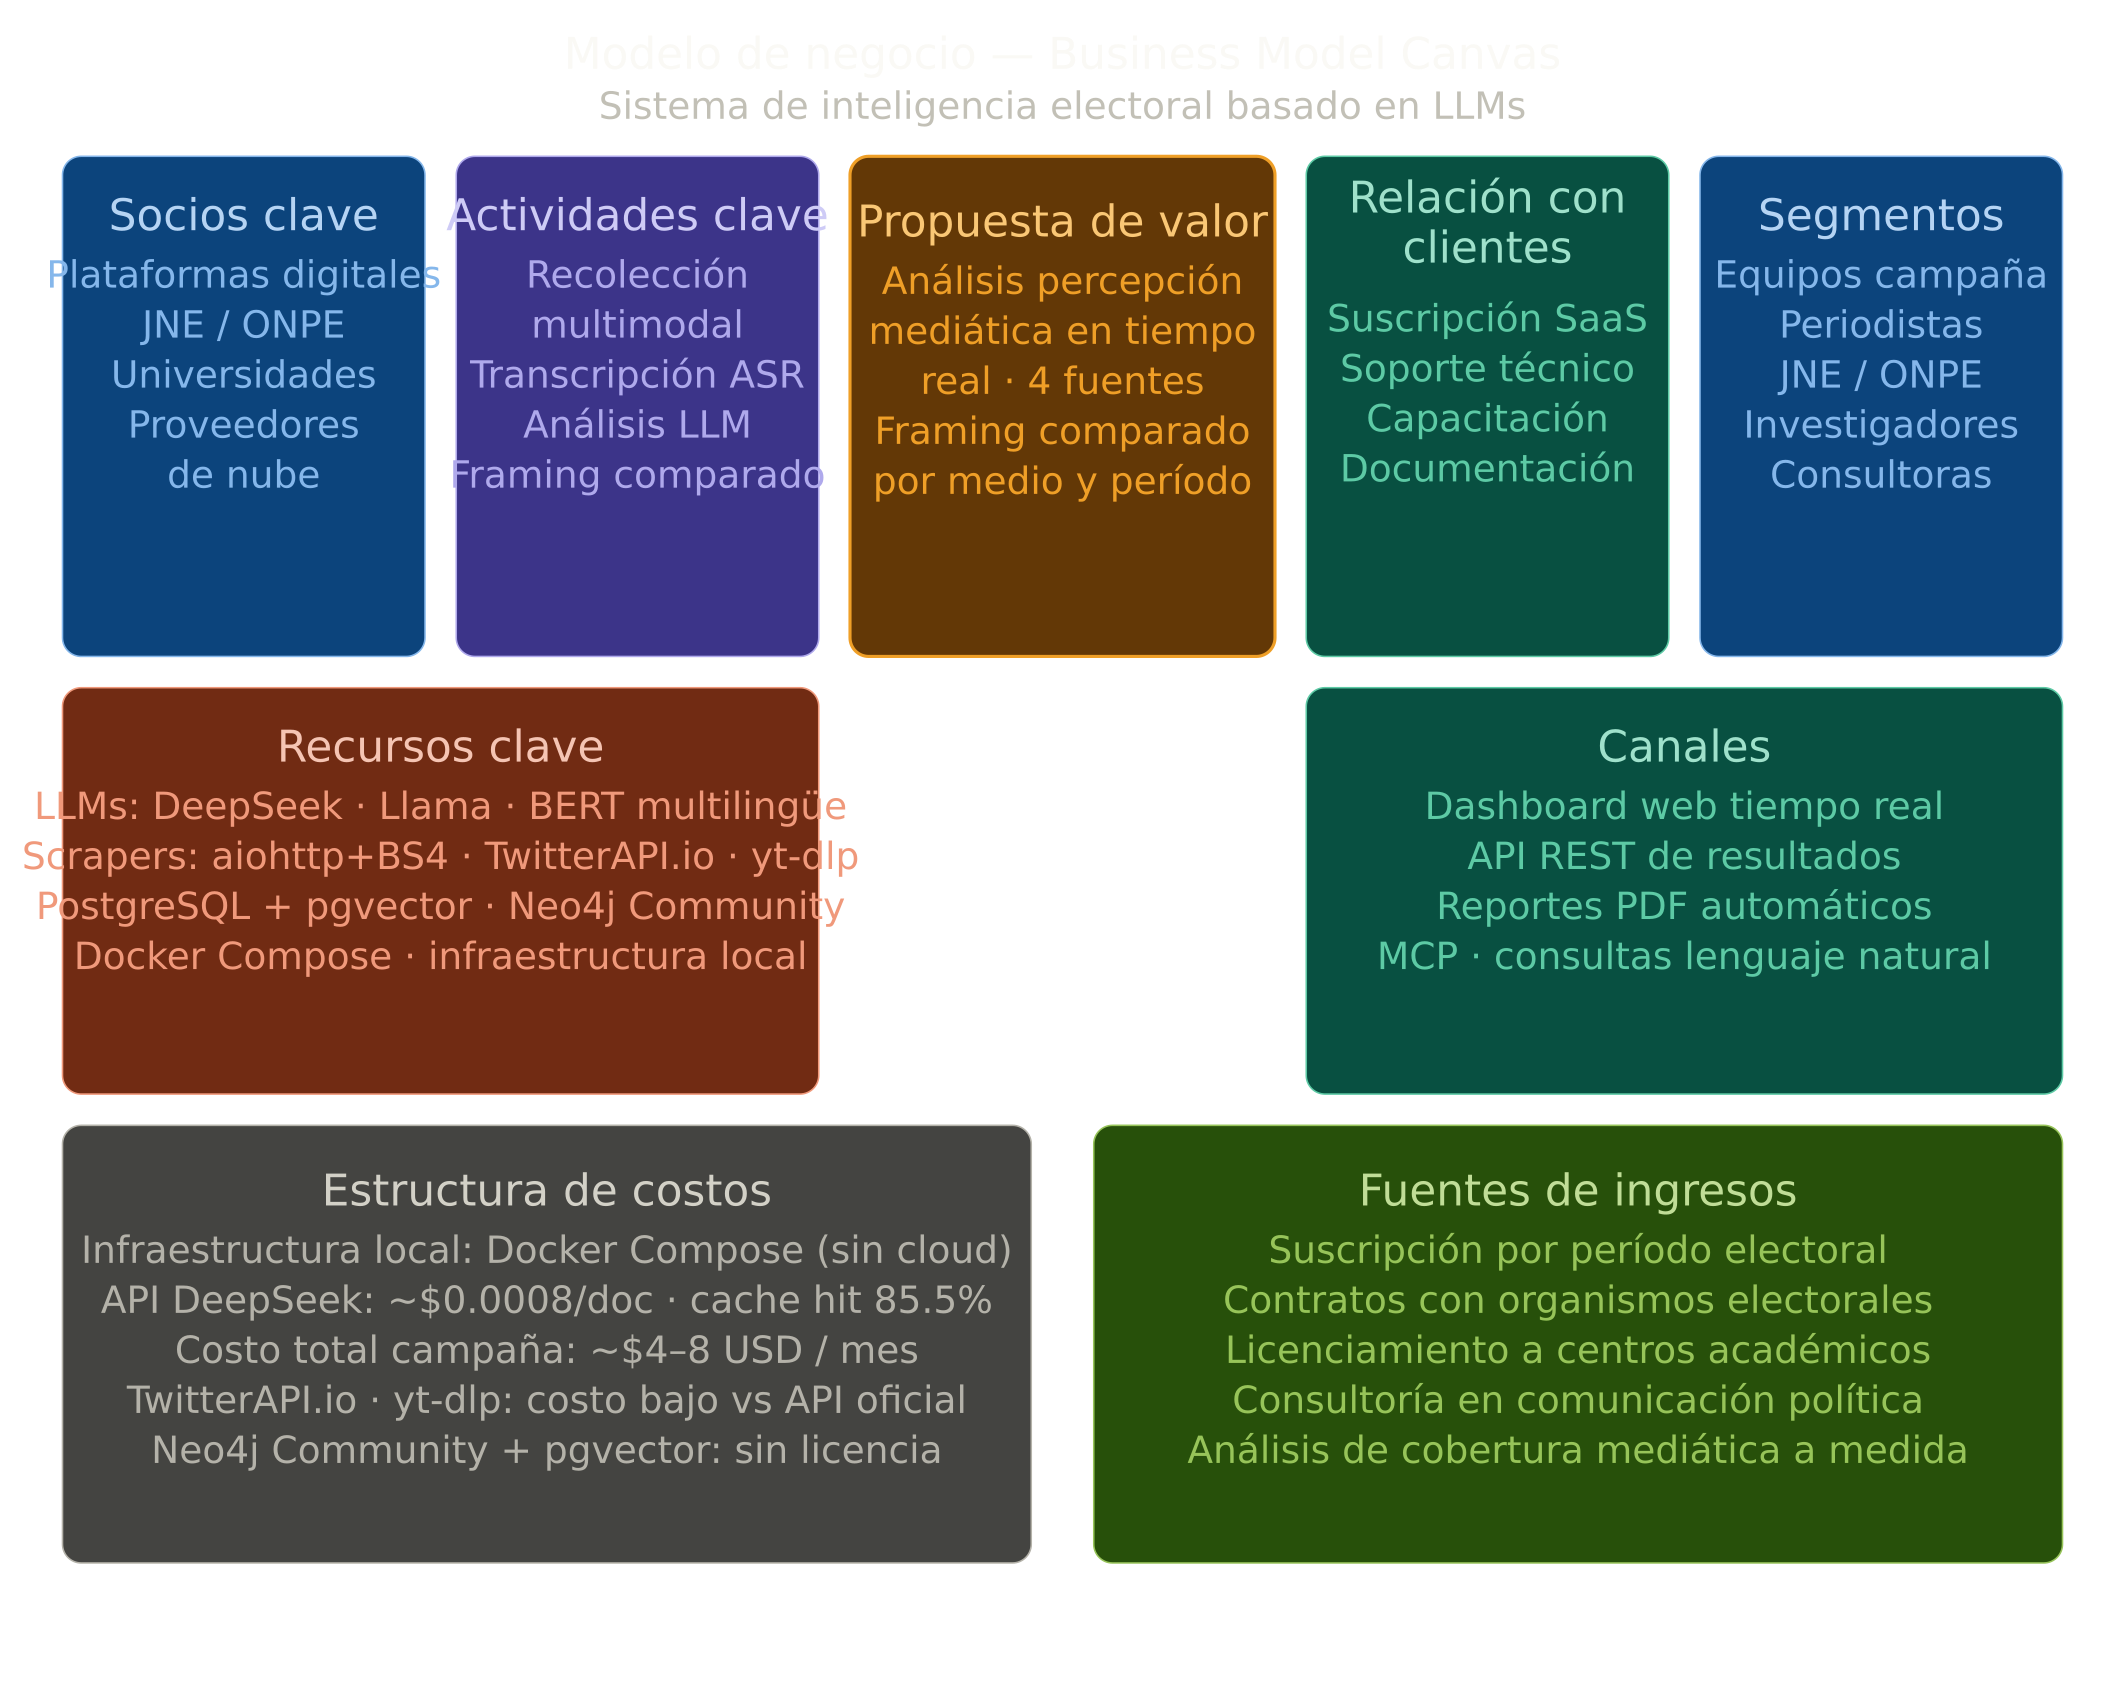
\includegraphics[width=0.92\textwidth]{2.5/figures/canvas_sistema.png}
        % ► NOTA PARA EL AUTOR: actualiza esta figura para reflejar
        %   la propuesta de valor centrada en "percepción proyectada por
        %   los medios" y las 4 fuentes en Recursos Clave. Ver notas_figuras.tex.
        \caption[Modelo CANVAS del sistema de inteligencia electoral basado en LLMs]{Modelo de negocio CANVAS del sistema de inteligencia electoral, mostrando la propuesta de valor centrada en el análisis de percepción mediática, segmentos de clientes, canales, recursos clave (4 fuentes multimodales), actividades clave y estructura de costos.\\
            Fuente: Elaboración propia.}
        \label{fig:canvas_sistema}
    \end{center}
\end{figure}

\section{Mapa de procesos actual}

\subsection{Descripción de los procesos}

El mapa de procesos del sistema de inteligencia electoral se estructura en tres niveles: procesos estratégicos, procesos operativos y procesos de soporte, cuya interacción se ilustra en la Figura \ref{fig:mapa_procesos}. Esta arquitectura de procesos garantiza que el flujo de datos —desde la recolección multimodal hasta la presentación de los indicadores de percepción mediática— sea continuo, trazable y de alta calidad.

\begin{figure}[!ht]
    \begin{center}
        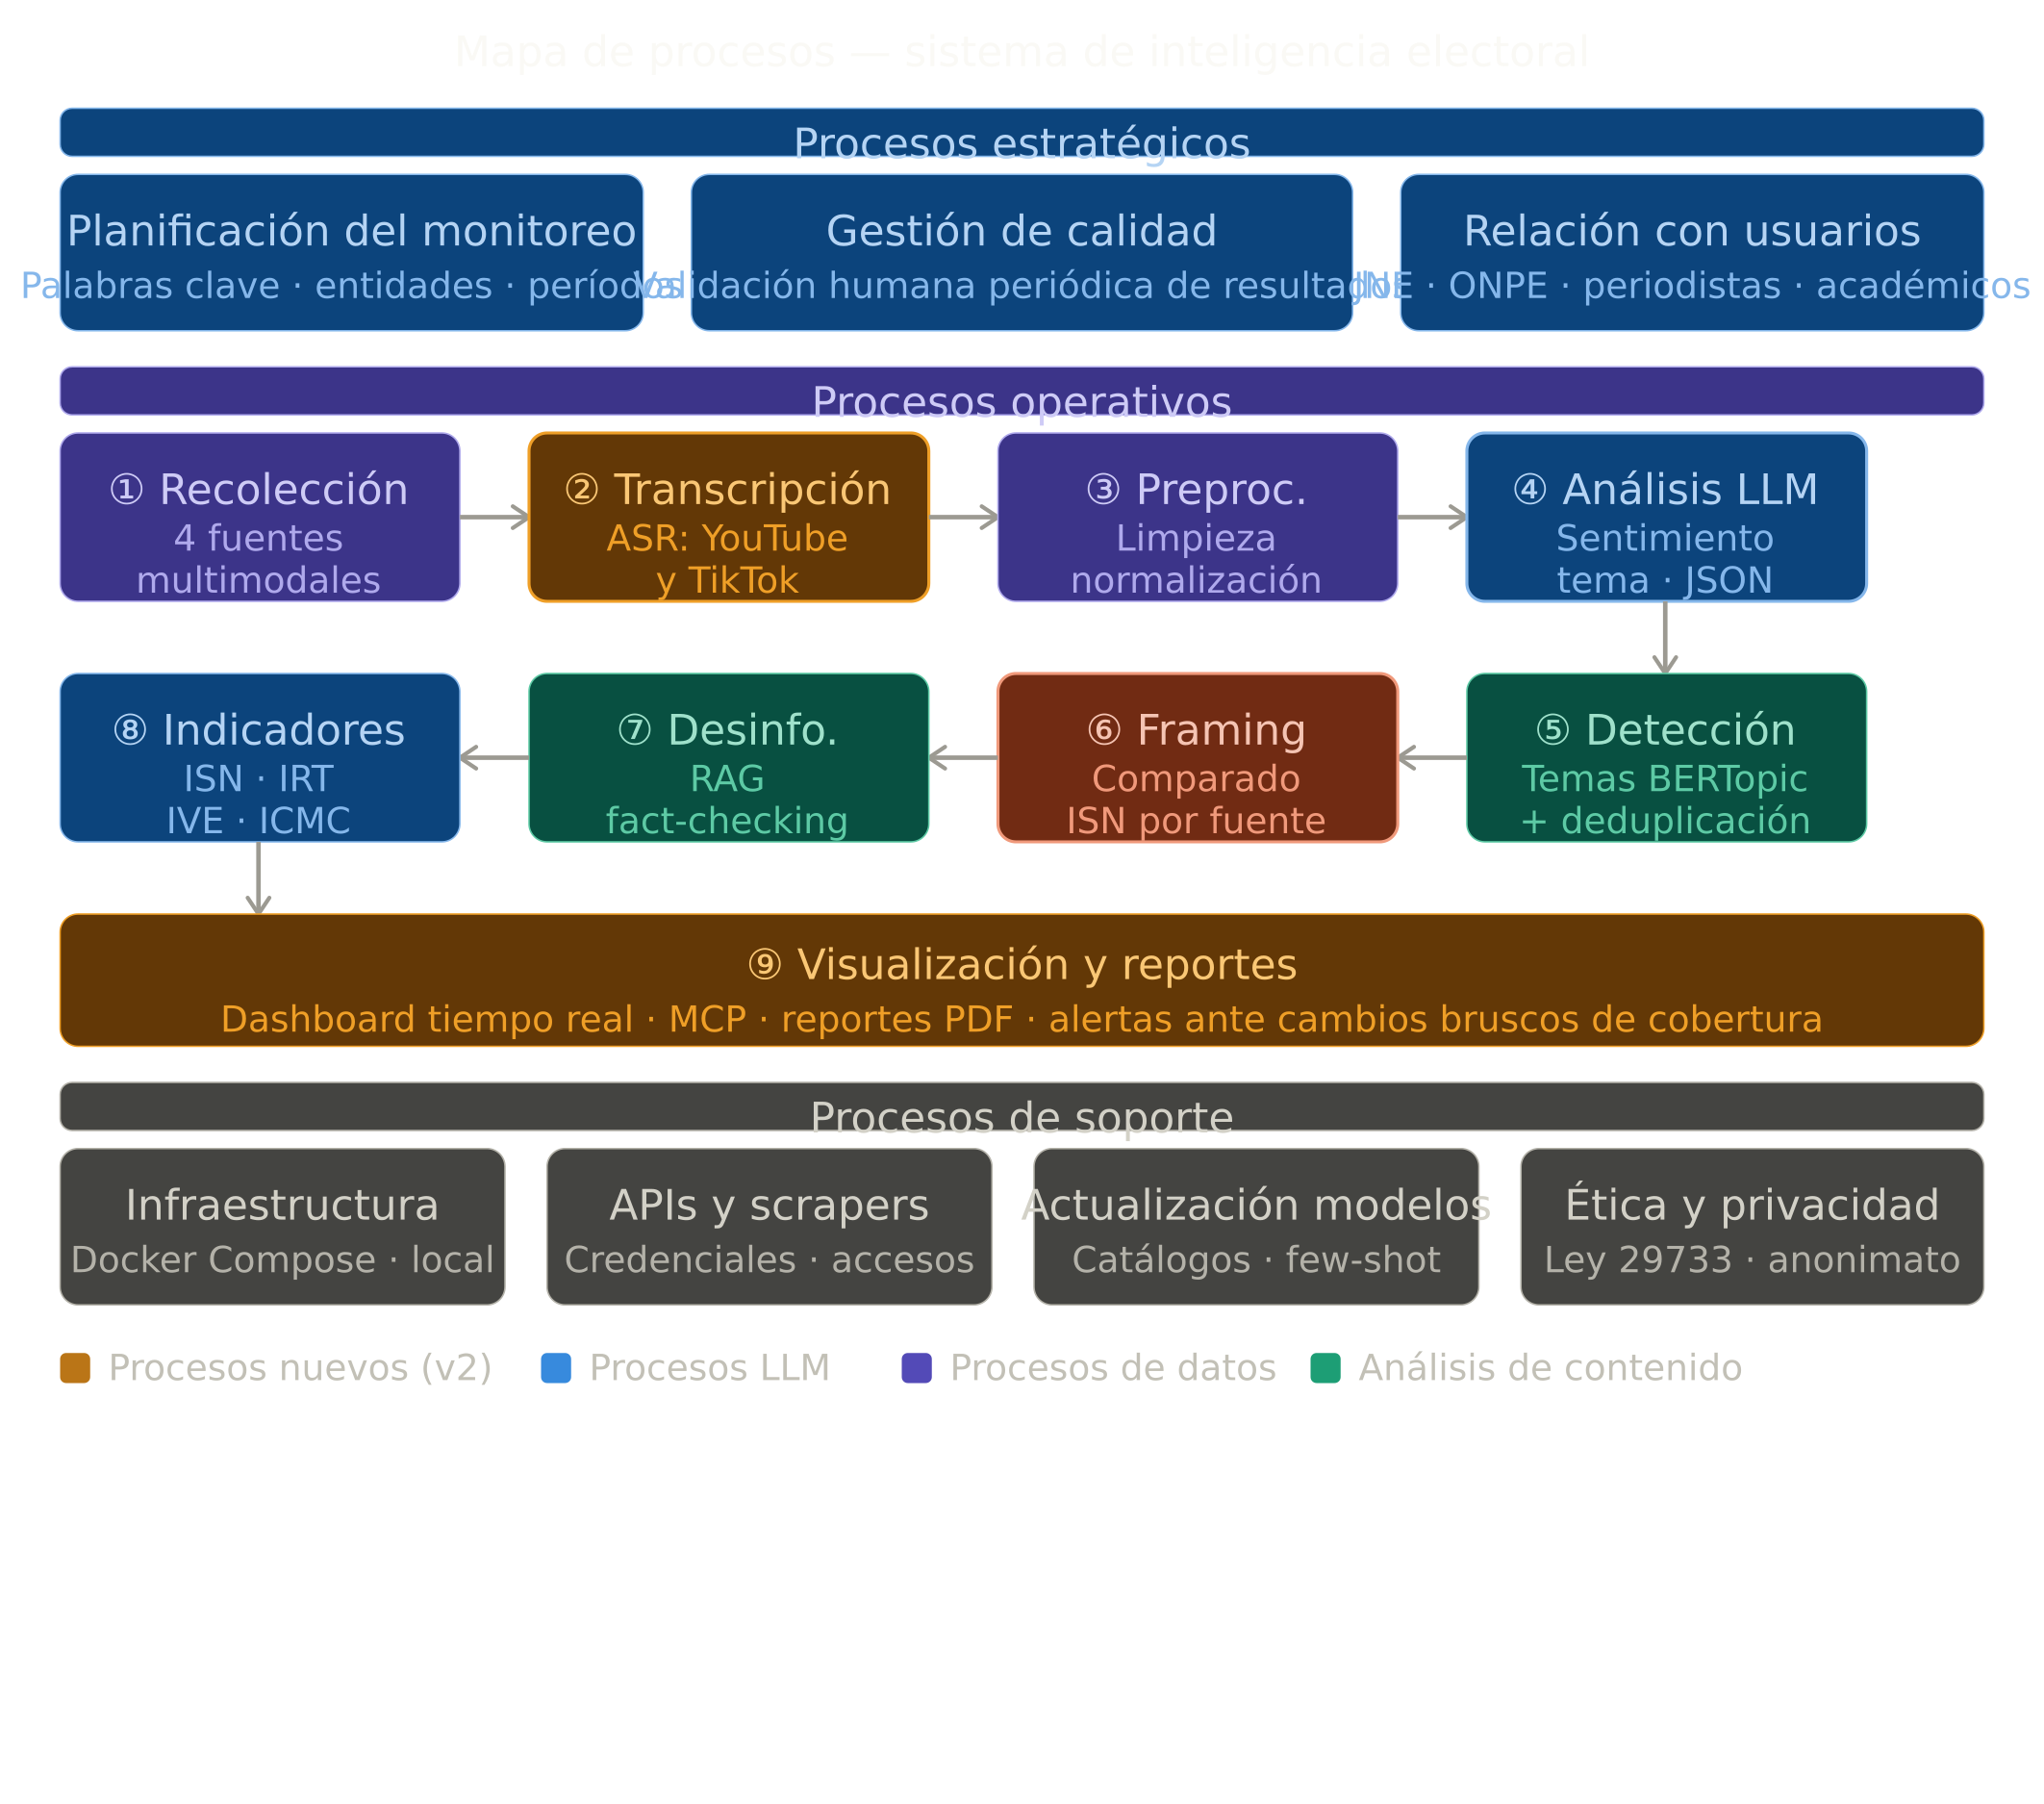
\includegraphics[width=0.95\textwidth]{2.5/figures/mapa_procesos.png}
        % ► NOTA PARA EL AUTOR: actualiza esta figura para incluir
        %   la transcripción audiovisual (YouTube/TikTok) como proceso
        %   operativo y el análisis de framing comparado como salida.
        %   Ver notas_figuras.tex.
        \caption[Mapa de procesos del sistema de inteligencia electoral multimodal]{Mapa de procesos del sistema de inteligencia electoral: procesos estratégicos de planificación y gestión de calidad, procesos operativos del pipeline multimodal (recolección, transcripción, análisis LLM, detección de temas, framing comparado) y procesos de soporte tecnológico y ético.\\
            Fuente: Elaboración propia.}
        \label{fig:mapa_procesos}
    \end{center}
\end{figure}

Los \textbf{procesos estratégicos} incluyen la planificación del monitoreo electoral (definición de palabras clave, medios a monitorear, períodos de análisis y entidades de interés), la gestión de la calidad de los resultados mediante validación humana periódica, y la gestión de las relaciones con los organismos electorales y los usuarios finales del sistema.

Los \textbf{procesos operativos} constituyen el núcleo del sistema y comprenden las siguientes etapas secuenciales:

\begin{itemize}
    \item \textbf{Recolección multimodal de datos}: Ingesta de artículos de noticias mediante scrapers aiohttp + BeautifulSoup de ocho portales; publicaciones de X/Twitter mediante TwitterAPI.io; videos y transcripciones de YouTube; y publicaciones y metadata de TikTok, todo ello filtrado por palabras clave electorales y cuentas de medios relevantes.

    \item \textbf{Transcripción de contenido audiovisual}: Conversión automática de audio a texto de los videos de YouTube y TikTok mediante modelos de reconocimiento de voz, generando transcripciones procesables por el LLM.

    \item \textbf{Preprocesamiento y limpieza de texto}: Eliminación de spam, duplicados y contenido irrelevante; normalización del texto en español (eliminación de URLs, menciones y caracteres especiales); detección de idioma y filtrado de publicaciones en español; almacenamiento en capa Bronze de la arquitectura Medallion.

    \item \textbf{Análisis de sentimientos y framing con LLM}: Clasificación de la polaridad (positivo / negativo / neutral), la emoción y el encuadre mediático de cada documento hacia las entidades políticas mencionadas, mediante prompts diseñados para el contexto de cobertura mediática electoral peruana en modalidad zero-shot y few-shot. La salida se almacena en capa Silver en formato JSON estructurado con campos para: fuente mediática, tipo de plataforma, candidato protagonista, actores secundarios, tema emergente, categoría, sentimiento por candidato y nivel de confianza.

    \item \textbf{Detección dinámica de temas}: Generación de embeddings semánticos con Sentence-BERT multilingüe, construcción de un menú de temas candidatos mediante retrieval multinivel (trending, semántico, léxico, por actor y por evento) y clasificación con LLM en categorías \textit{exact}, \textit{alias} o \textit{new} dentro de un catálogo incremental, con consolidación y deduplicación semántica diaria. La deduplicación entre fuentes heterogéneas se realiza mediante el pipeline de tres etapas descrito en el marco teórico.

    \item \textbf{Análisis de cobertura mediática comparada}: Cálculo del Índice de Sentimiento Neto (ISN) desagregado por fuente mediática y plataforma, identificación de divergencias de framing entre medios y construcción de los perfiles de cobertura por candidato y período.

    \item \textbf{Detección de desinformación}: Verificación automática de los contenidos con mayor viralidad mediante técnicas de RAG, confrontando el contenido con fuentes verificadas y bases de datos de fact-checking.

    \item \textbf{Cálculo de indicadores y generación de reportes}: Cómputo del ISN, IRT, IVE e ICMC por entidad política, fuente mediática y período de tiempo; generación automática de reportes diarios y alertas ante cambios bruscos de cobertura. Los resultados se materializan en vistas Gold de la arquitectura Medallion.
\end{itemize}

Los \textbf{procesos de soporte} incluyen la gestión de la infraestructura tecnológica local (Docker Compose), el monitoreo del rendimiento de los modelos LLM, la gestión de las credenciales y permisos de las APIs y scrapers, el mantenimiento y actualización de los catálogos de entidades electorales, y la supervisión ética y de privacidad de los datos procesados.
\chapter{Metodología de la Investigación}
 
\section{Diseño de la investigación}
 
En esta sección se explica cuál fue el diseño, el tipo y el enfoque del trabajo de
investigación, así como también la población, la muestra y la operacionalización de
variables.
 
\subsection{Tipo de la investigación}
 
Para determinar el tipo de la investigación, primero fue necesario definir el actual
trabajo como \textbf{Diseño Experimental} ya que, según \cite{bk_hernandez2014metodologia}
en su libro \citetitle{bk_hernandez2014metodologia}, se pretende establecer el posible
efecto de una causa que se manipula. Dentro de esta categoría se clasifica como
\textbf{Diseño Experimental Puro}, ya que se manipularon intencionalmente una o más
variables independientes —específicamente la configuración del pipeline de análisis con
LLMs— con la finalidad de medir el efecto que estas generan en la variable dependiente:
la exactitud en la clasificación del sentimiento y la coherencia semántica en la detección
de temas relevantes en el ecosistema digital electoral peruano.
 
\subsection{Enfoque de la investigación}
 
El presente trabajo tuvo un \textbf{enfoque cuantitativo} ya que, según
\cite{bk_hernandez2014metodologia} en su libro \citetitle{bk_hernandez2014metodologia},
este enfoque utiliza la recolección de datos para probar hipótesis con base en la medición
numérica y el análisis estadístico, con el fin de establecer pautas de comportamiento y
probar teorías. Esto se refleja en los 10 pasos del proceso cuantitativo descritos por el
anterior autor y que fueron aplicados en la investigación, desde la concepción de la idea
hasta la elaboración del reporte de resultados. En el presente trabajo, las métricas de
exactitud, coherencia temática y latencia de procesamiento permiten evaluar de forma
objetiva el desempeño del sistema de inteligencia electoral propuesto.
 
\subsection{Población}
 
La población fue el conjunto de todas las publicaciones digitales en español relacionadas
con el proceso electoral peruano, generadas en plataformas de redes sociales (X/Twitter),
portales de noticias digitales y canales de YouTube durante el período de campaña
presidencial analizado.
 
\subsection{Muestra}
 
La muestra estuvo conformada por publicaciones recolectadas de tres fuentes de datos
durante el período electoral comprendido entre los meses de enero y junio del año en
curso: (1) artículos y noticias digitales de los principales portales de prensa peruanos;
(2) comentarios de usuarios en los videos de YouTube de los candidatos y programas
periodísticos de cobertura electoral; y (3) tweets y publicaciones de X/Twitter
relacionados con los candidatos presidenciales, filtrados mediante palabras clave
electorales y hashtags de campaña. El criterio de delimitación temporal obedeció a la
necesidad de capturar el período de mayor actividad del ecosistema digital electoral,
excluyendo etapas de baja intensidad que distorsionarían los patrones de sentimiento y
emergencia de temas.
 
\subsection{Operacionalización de variables}
 
En la Tabla \ref{4:table1} se presenta la operacionalización de variables para la
investigación.
 
\begin{longtable}{M{3cm}M{4.2cm}M{3.6cm}M{4.8cm}}
    \caption[Matriz de operacionalización de variables]{Matriz de operacionalización de variables.}
    \label{4:table1}
    \centering
    \small
    \tabularnewline \specialrule{.1em}{.05em}{.05em}
    VARIABLE & DIMENSIÓN & INDICADOR & CÁLCULO \\
    \specialrule{.1em}{.05em}{.05em}
 
    % Variable independiente
    \multirow{8}{3cm}[-5ex]{\centering Independiente: Sistema de Inteligencia Electoral con LLM}
    & \multirow{6}{4.2cm}[-1ex]{\centering Modelo LLM de Análisis}
    & \multicolumn{2}{c}{\centering Configuración del pipeline de análisis} \\
    \cline{3-4}
    & & \multirow{5}{3.6cm}[0ex]{\centering Efectividad del análisis con LLM}
    & Exactitud en clasificación de sentimiento \\
    \cline{4-4}
    & & & Coherencia semántica de temas (C\textsubscript{v}) \\
    \cline{4-4}
    & & & Índice de Sentimiento Neto (ISN) \\
    \cline{4-4}
    & & & Índice de Relevancia Temática (IRT) \\
    \cline{4-4}
    & & & Latencia de procesamiento (ms) \\
    \cline{2-4}
    & Arquitectura del pipeline
    & \multicolumn{2}{c}{\thead{Complejidad e integridad\\del pipeline de procesamiento}} \\
 
    \hline
 
    % Variable dependiente
    \multirow{8}{3cm}[-5ex]{\centering Dependiente: Percepción pública nacional en el ecosistema digital}
    & \multirow{3}{4.2cm}[-2ex]{\centering Sentimiento ciudadano}
    & \multirow{2}{3.6cm}[0ex]{\centering Polaridad de sentimiento}
    & $Positivo: S(d,e) > 0$ \\
    \cline{4-4}
    & & & $Negativo: S(d,e) < 0$ \\
    \cline{3-4}
    & & Intensidad del sentimiento & Score continuo $[-1, 1]$ \\
    \cline{2-4}
    & \multirow{5}{4.2cm}[-2ex]{\centering Conversación digital electoral}
    & \multirow{2}{3.6cm}[0ex]{\centering Metainformación del corpus}
    & Volumen de publicaciones por período \\
    \cline{4-4}
    & & & Distribución por fuente de datos \\
    \cline{3-4}
    & & Temas relevantes & Número y coherencia de temas detectados \\
    \cline{3-4}
    & & \multirow{2}{3.6cm}[0ex]{\centering Evolución temporal}
    & Velocidad de emergencia de temas \\
    \cline{4-4}
    & & & Cambios de sentimiento por evento electoral \\
 
    \specialrule{.1em}{.05em}{.05em}
\end{longtable}
\begin{flushleft}
    \small Fuente: Elaboración propia.
\end{flushleft}
 
El trabajo busca resolver el problema de análisis de percepción pública nacional en
ecosistemas digitales electorales, implementando un pipeline automatizado de inteligencia
electoral que integra análisis de sentimientos con LLMs y detección dinámica de temas
mediante BERTopic sobre un corpus multicanal de publicaciones en español.
 
La variable dependiente —la percepción pública nacional— se operacionaliza a través del
sentimiento expresado en publicaciones digitales hacia cada candidato presidencial,
desagregado por fuente de información, período temporal y tema relevante asociado.
Siguiendo la metodología GraphRAG descrita en la arquitectura del sistema, un mismo
segmento de texto puede expresar sentimientos distintos hacia distintos candidatos, lo que
permite capturar la complejidad real del discurso político ciudadano a nivel de aspecto
(\textit{Aspect-Based Sentiment Analysis}).
 
\section{Técnicas de recolección de datos}
 
Los conjuntos de datos recolectados para la investigación se componen de variables
cuantitativas —como el score continuo de sentimiento $[-1, 1]$, el volumen de
publicaciones por período y la frecuencia de temas— y variables cualitativas —como el
texto de las publicaciones, los fragmentos clave que justifican el sentimiento y las
etiquetas de temas generadas por el LLM—. Para obtener los tres corpus principales, se
siguió el flujo de la Figura \ref{4:fig1}.
 
\begin{figure}[!ht]
    \begin{center}
        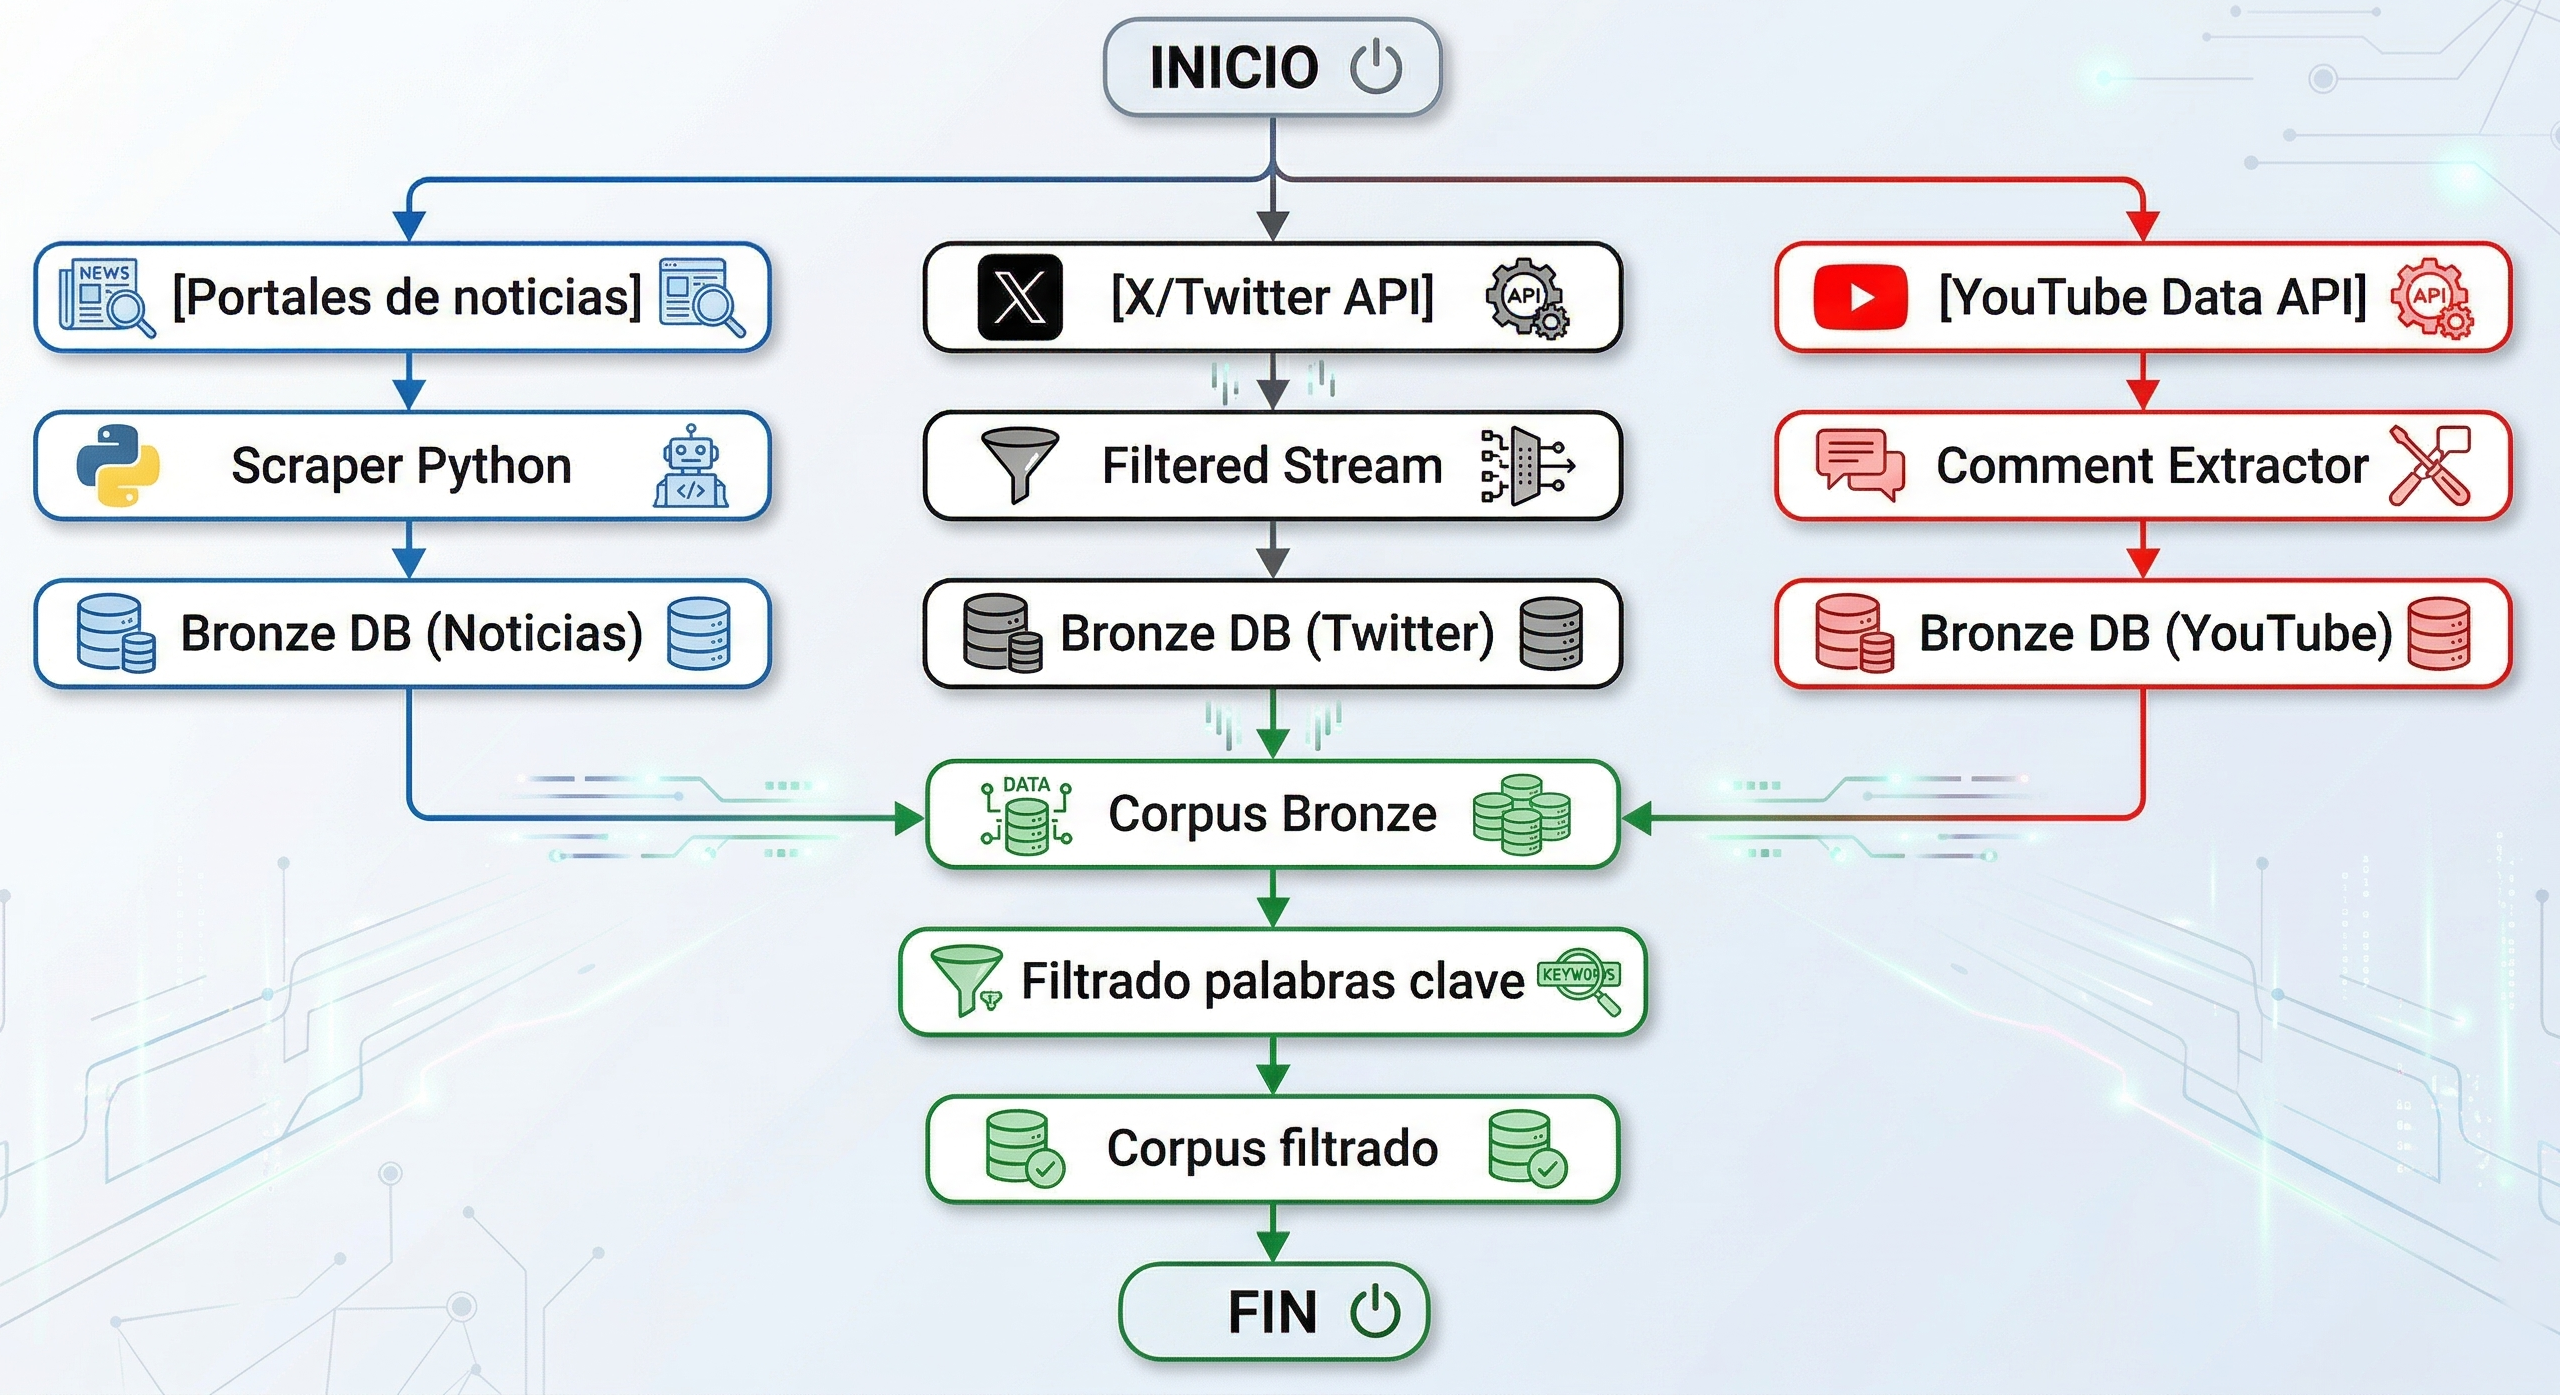
\includegraphics[width=0.90\textwidth]{3/figures/flujo_recoleccion.png}
        \caption[Flujograma de recolección de los conjuntos de datos del corpus electoral]{Flujograma de recolección de los conjuntos de datos del corpus electoral: noticias digitales, comentarios de YouTube y tweets de X/Twitter, con sus respectivos procesos de filtrado y almacenamiento en la capa Bronze de la arquitectura Medallion.\\
            Fuente: Elaboración propia.}
        \label{4:fig1}
    \end{center}
\end{figure}
 
Asimismo, para identificar y filtrar las publicaciones relevantes para el análisis, se
definió un diccionario de palabras clave y aliases electorales que incluye los nombres
completos, apodos, partidos y hashtags de los candidatos presidenciales en liza, así como
términos relacionados con los principales temas de la campaña: economía, seguridad,
educación, salud, corrupción y gobernabilidad.
 
\section{Técnicas para el procesamiento y análisis de la información}
 
\subsection{Metodología de implementación de la solución}
 
Como se explicó en el Capítulo II del presente trabajo, dentro de los sistemas de
analítica de negocio, Big Data y Minería de Datos, las tres metodologías más usadas son
CRISP-DM, SEMMA y KDD \parencite{tec_braulio2015metodologiasdm}. Para elegir la
metodología de implementación, se elaboró la Tabla \ref{4:table2} con el fin de comparar
las utilizadas por los autores en los antecedentes de esta investigación.
 
\vspace{2ex}
\begingroup
\renewcommand\arraystretch{0.3}
\begin{longtable}{M{3cm}M{2.5cm}M{2.5cm}M{6cm}}
    \caption[Cuadro comparativo para la selección de la metodología]{Cuadro comparativo para la selección de la metodología de implementación.}
    \label{4:table2}
    \footnotesize
    \centering
    \small
    \tabularnewline \specialrule{.1em}{.05em}{.05em}
    Metodología & Cantidad de referencias & Número de pasos & Nombre de los pasos \\
    \specialrule{.1em}{.05em}{.05em}
    {CRISP-DM}
    & 2
    & 6
    & \setlist{nolistsep}
    \begin{itemize}[label={--},nosep,noitemsep,leftmargin=*,topsep=0pt,partopsep=0pt]
        \item Comprensión del negocio.
        \item Comprensión de los datos.
        \item Preparación de los datos.
        \item Modelado.
        \item Evaluación.
        \item Despliegue.
    \end{itemize}
    \\
    \hline
    {Grupo A}
    & 2
    & 6
    & \setlist{nolistsep}
    \begin{itemize}[label={--},nosep,noitemsep,leftmargin=*,topsep=0pt,partopsep=0pt]
        \item Formulación del problema.
        \item Recolección de datos multicanal.
        \item Preprocesamiento de texto.
        \item Análisis con LLM.
        \item Evaluación.
        \item Despliegue.
    \end{itemize}
    \\
    \hline
    {Grupo B}
    & 2
    & 5
    & \setlist{nolistsep}
    \begin{itemize}[label={--},nosep,noitemsep,leftmargin=*,topsep=0pt,partopsep=0pt]
        \item Recolección de datos.
        \item Preprocesamiento y filtrado.
        \item Análisis de sentimientos.
        \item Detección de temas.
        \item Evaluación.
    \end{itemize}
    \\
    \hline
    {Grupo C}
    & 2
    & 5
    & \setlist{nolistsep}
    \begin{itemize}[label={--},nosep,noitemsep,leftmargin=*,topsep=0pt,partopsep=0pt]
        \item Formulación del problema.
        \item Recolección de datos.
        \item Preprocesamiento de datos.
        \item Modelado y análisis.
        \item Evaluación.
    \end{itemize}
    \\
    \hline
    {Grupo D}
    & 1
    & 4
    & \setlist{nolistsep}
    \begin{itemize}[label={--},nosep,noitemsep,leftmargin=*,topsep=0pt,partopsep=0pt]
        \item Recolección de datos.
        \item Preprocesamiento.
        \item Análisis LLM y clustering.
        \item Evaluación.
    \end{itemize}
    \\
    \specialrule{.1em}{.05em}{.05em}
\end{longtable}
\endgroup
\begin{flushleft}
    \small Fuente: Elaboración propia.
\end{flushleft}
 
De las tres metodologías mencionadas por \citeauthor{tec_braulio2015metodologiasdm},
la mayoría de los antecedentes revisados siguen secuencias de actividades comprendidas
dentro de CRISP-DM, incluyendo fases de comprensión del negocio, recolección y
preparación de datos, modelado y evaluación. Además, las siguientes características de la
literatura influyeron en la elección de la metodología CRISP-DM para el presente trabajo:
 
\begin{itemize}
    \item La metodología contempla entre sus fases la comprensión del negocio además
    de la parte técnica. Esta fase es crucial ya que en ella se define el problema a resolver
    —la falta de un sistema de análisis automatizado de percepción pública electoral en
    tiempo real— y se establecen los objetivos del sistema.
 
    \item Ayuda a los responsables del proyecto en la planificación y toma de decisiones
    (fase de Despliegue) a partir de los resultados obtenidos, convirtiendo los indicadores
    del sistema en oportunidades para mejorar la campaña de inteligencia electoral.
 
    \item Evalúa en todo el proceso los datos y configuraciones del modelo con el fin de
    construir el mejor pipeline. Estas evaluaciones son importantes para interpretar los
    resultados y tomar decisiones sobre la arquitectura del sistema.
 
    \item A diferencia de SEMMA, que comienza directamente con el muestreo sin hacer
    hincapié en la comprensión del contexto, y de KDD, cuyo enfoque es más técnico y
    orientado a métricas sin considerar el entorno del negocio, CRISP-DM contempla
    explícitamente la formulación del problema, presente en el actual trabajo.
\end{itemize}
 
Cada una de las fases de la metodología seleccionada, adaptada al contexto de la
inteligencia electoral con LLMs, se detalla en la Figura \ref{4:fig2}.
 
\begin{figure}[!ht]
    \begin{center}
        \includegraphics[width=1\textwidth]{3/figures/metodologia_crispdm.png}
        \caption[Metodología CRISP-DM adaptada al sistema de inteligencia electoral con LLMs]{Metodología CRISP-DM adaptada al sistema de inteligencia electoral con LLMs, mostrando las seis fases, su carácter iterativo y los entregables de cada etapa.\\
            Fuente: Elaboración propia.}
        \label{4:fig2}
    \end{center}
\end{figure}
 
Durante el proceso de implementación de la metodología, se definió construir un pipeline
de análisis multicanal que integra análisis de sentimientos con LLMs, detección dinámica
de temas con BERTopic y un grafo de conocimiento con Neo4j, arquitectura denominada
\textbf{GraphRAG Electoral}. De acuerdo a la literatura de los antecedentes revisados,
se analizaron las siguientes posibles fuentes de datos a incorporar:
 
\begin{itemize}
    \item \textbf{Noticias digitales}: \cite{pr_alvarez2023llm_political}, \cite{pr_mendonca2025bertopic_political}, \cite{pr_alvi2023twitter_election_review}.
    \item \textbf{Publicaciones en X/Twitter}: \cite{pr_gujral2024llm_elections}, \cite{pr_alvi2023twitter_election_review}, \cite{pr_mendonca2025bertopic_political}.
    \item \textbf{Comentarios de YouTube}: \cite{pr_chen2024combating_misinformation}.
    \item \textbf{Datos de encuestas electorales}: \cite{pr_gujral2024llm_elections}.
\end{itemize}
 
De las anteriores fuentes, los datos de encuestas electorales no fueron incluidos en el
pipeline principal de procesamiento ya que se utilizan exclusivamente como conjunto de
validación para calibrar los indicadores del sistema, y no como datos de entrada para el
análisis de sentimientos. Finalmente, fueron seleccionadas las tres fuentes principales
—noticias digitales, X/Twitter y comentarios de YouTube— cuya arquitectura de
recolección, procesamiento y análisis se detalla en las subsecciones siguientes.
 
El marco de trabajo del sistema propuesto, denominado \textbf{Pipeline GraphRAG
Electoral}, se estructura según la arquitectura Medallion en tres capas de datos
(Bronze, Silver y Gold) y cinco etapas de procesamiento, como se aprecia en la
Figura \ref{4:fig3}.
 
\begin{figure}[!ht]
    \begin{center}
        \includegraphics[width=0.92\textwidth]{3/figures/framework_graphrag.png}
        \caption[Marco de trabajo del Pipeline GraphRAG Electoral propuesto]{Marco de trabajo del Pipeline GraphRAG Electoral: arquitectura Medallion con tres capas de datos (Bronze, Silver, Gold) y cinco etapas de procesamiento desde la ingesta hasta la generación de indicadores de percepción pública.\\
            Fuente: Elaboración propia.}
        \label{4:fig3}
    \end{center}
\end{figure}
 
\subsubsection{Comprensión del negocio}
 
En la primera fase, se definió el problema a partir de comprender el contexto del proceso
electoral peruano y la necesidad de un sistema automatizado de inteligencia electoral. Las
actividades y tareas de esta fase se presentan en la Tabla \ref{4:table3}.
 
\vspace{2ex}
\begingroup
\renewcommand\arraystretch{0.3}
\begin{longtable}{m{5cm}m{5cm}M{5cm}}
    \caption[Actividades de la fase Comprensión del negocio]{Actividades de la fase Comprensión del negocio.}
    \label{4:table3}
    \footnotesize
    \small
    \tabularnewline \specialrule{.1em}{.05em}{.05em}
    \centering Actividades & \centering Descripción & Tareas \\
    \specialrule{.1em}{.05em}{.05em}
    Definir problema, objetivos e hipótesis.
    & Definición del problema central, los objetivos generales y específicos, y las hipótesis de investigación.
    & \setlist{nolistsep}
    \begin{itemize}[label={--},nosep,noitemsep,leftmargin=*,topsep=0pt,partopsep=0pt]
        \item Identificar la brecha en el análisis de percepción electoral digital.
        \item Definir los objetivos del sistema de inteligencia electoral.
        \item Formular las hipótesis del trabajo.
    \end{itemize}
    \\
    \hline
    Desarrollar la literatura de la investigación.
    & Revisión de antecedentes y trabajos previos sobre análisis de sentimientos político, LLMs y detección de temas.
    & \setlist{nolistsep}
    \begin{itemize}[label={--},nosep,noitemsep,leftmargin=*,topsep=0pt,partopsep=0pt]
        \item Buscar publicaciones académicas sobre LLMs en contextos electorales.
        \item Buscar material sobre BERTopic y GraphRAG aplicado a datos políticos.
    \end{itemize}
    \\
    \hline
    Definir metodología y arquitectura del sistema.
    & Selección de la metodología de implementación y diseño de la arquitectura del pipeline.
    & \setlist{nolistsep}
    \begin{itemize}[label={--},nosep,noitemsep,leftmargin=*,topsep=0pt,partopsep=0pt]
        \item Evaluar metodologías de la literatura.
        \item Seleccionar la metodología CRISP-DM.
        \item Diseñar la arquitectura Medallion del sistema.
    \end{itemize}
    \\
    \specialrule{.1em}{.05em}{.05em}
\end{longtable}
\endgroup
\begin{flushleft}
    \small Fuente: Elaboración propia.
\end{flushleft}
 
\textbf{Actividad 1: Definir problema, objetivos e hipótesis}
 
En esta actividad se detalla cómo se identificó la brecha existente en el análisis automatizado de la percepción pública electoral digital en el Perú, se formularon los objetivos de la investigación y se plantearon las hipótesis que guían el trabajo experimental.
 
\textbf{Entregable}: Problema, objetivos e hipótesis definidos.
 
\textbf{Actividad 2: Desarrollar la literatura de la investigación}
 
A partir de los objetivos definidos, se realizó la búsqueda de antecedentes académicos relacionados con el uso de LLMs en contextos electorales, minería de sentimientos político en español, detección dinámica de temas con BERTopic y sistemas GraphRAG. Se elaboró el marco teórico y conceptual descritos en el Capítulo II del presente trabajo.
 
\textbf{Entregable}: Marco teórico, antecedentes y conceptos operacionales de la investigación.
 
\textbf{Actividad 3: Definir metodología y arquitectura del sistema}
 
Luego de revisar los antecedentes y comparar las metodologías utilizadas por cada autor, se seleccionó CRISP-DM como metodología de implementación y se diseñó la arquitectura Medallion del pipeline GraphRAG Electoral.
 
\textbf{Entregable}: Metodología de implementación y arquitectura del sistema.
 
\subsubsection{Comprensión de los datos}
 
La segunda fase abarcó la recolección y el análisis estadístico exploratorio del corpus
electoral multicanal. Los datos utilizados comprenden publicaciones de tres fuentes
principales recolectadas durante el período de campaña presidencial. La lista de
actividades y tareas se presenta en la Tabla \ref{4:table4}.
 
\vspace{2ex}
\begingroup
\renewcommand\arraystretch{0.3}
\begin{longtable}{m{4cm}m{5.5cm}M{5.5cm}}
    \caption[Actividades de la fase Comprensión de los datos]{Actividades de la fase Comprensión de los datos.}
    \label{4:table4}
    \footnotesize
    \small
    \tabularnewline \specialrule{.1em}{.05em}{.05em}
    \centering Actividades & \centering Descripción & Tareas \\
    \specialrule{.1em}{.05em}{.05em}
    Construir corpus de noticias digitales.
    & Construcción del corpus de artículos y titulares de los principales portales de prensa peruanos (capa Bronze).
    & \setlist{nolistsep}
    \begin{itemize}[label={--},nosep,noitemsep,leftmargin=*,topsep=0pt,partopsep=0pt]
        \item Diseñar scrapers para portales de noticias objetivo.
        \item Recolectar artículos con URL, fecha, titular y texto.
        \item Almacenar datos crudos en capa Bronze.
    \end{itemize}
    \\
    \hline
    Construir corpus de X/Twitter.
    & Construcción del corpus de tweets relacionados con los candidatos presidenciales mediante la API de X.
    & \setlist{nolistsep}
    \begin{itemize}[label={--},nosep,noitemsep,leftmargin=*,topsep=0pt,partopsep=0pt]
        \item Configurar conexión con la API Filtered Stream de X.
        \item Definir palabras clave, hashtags y cuentas de interés.
        \item Almacenar tweets con metadatos en capa Bronze.
    \end{itemize}
    \\
    \hline
    Construir corpus de YouTube.
    & Construcción del corpus de comentarios de usuarios en videos electorales de YouTube.
    & \setlist{nolistsep}
    \begin{itemize}[label={--},nosep,noitemsep,leftmargin=*,topsep=0pt,partopsep=0pt]
        \item Identificar videos electorales mediante YouTube Data API.
        \item Recolectar comentarios con ID de usuario y fecha.
        \item Almacenar comentarios crudos en capa Bronze.
    \end{itemize}
    \\
    \hline
    Realizar análisis exploratorio del corpus.
    & Análisis estadístico y exploratorio de las variables del corpus para cada fuente de datos.
    & \setlist{nolistsep}
    \begin{itemize}[label={--},nosep,noitemsep,leftmargin=*,topsep=0pt,partopsep=0pt]
        \item Describir distribución temporal y por fuente.
        \item Analizar longitud de textos y vocabulario.
        \item Identificar candidatos más mencionados.
    \end{itemize}
    \\
    \specialrule{.1em}{.05em}{.05em}
\end{longtable}
\endgroup
\begin{flushleft}
    \small Fuente: Elaboración propia.
\end{flushleft}
 
\textbf{Actividad 1: Construir corpus de noticias digitales}
 
De acuerdo a la Figura \ref{4:fig1}, en esta actividad se construyó el corpus de artículos de noticias digitales mediante scrapers diseñados en Python para los portales de prensa peruanos seleccionados. El proceso de recolección siguió el flujo de la Figura \ref{4:fig4}.
 
\begin{figure}[!ht]
    \begin{center}
        \includegraphics[width=0.80\textwidth]{3/figures/flujo_scraping_noticias.png}
        \caption[Proceso de recolección del corpus de noticias digitales]{Proceso de recolección del corpus de noticias digitales: desde la identificación de portales objetivo hasta el almacenamiento en la capa Bronze de la arquitectura Medallion.\\
            Fuente: Elaboración propia.}
        \label{4:fig4}
    \end{center}
\end{figure}
 
\textbf{Entregable}: Corpus de noticias digitales con URL, fecha, portal de origen, titular y texto completo del artículo.
 
\textbf{Actividad 2: Construir corpus de X/Twitter}
 
Una vez configurada la conexión con la API Filtered Stream de X, se definió el conjunto de palabras clave, hashtags y cuentas de candidatos que activan la captura en tiempo real. El proceso de recolección se realizó según el flujo de la Figura \ref{4:fig5}.
 
\begin{figure}[!ht]
    \begin{center}
        \includegraphics[width=0.80\textwidth]{3/figures/flujo_api_twitter.png}
        \caption[Proceso de recolección del corpus de X/Twitter mediante API Filtered Stream]{Proceso de recolección del corpus de X/Twitter: configuración de reglas de filtrado, captura en streaming y almacenamiento con metadatos en capa Bronze.\\
            Fuente: Elaboración propia.}
        \label{4:fig5}
    \end{center}
\end{figure}
 
\textbf{Entregable}: Corpus de tweets con ID, texto, fecha, número de retweets y menciones a candidatos.
 
\textbf{Actividad 3: Construir corpus de YouTube}
 
Mediante la YouTube Data API, se identificaron los videos electorales más relevantes y se recolectaron sus comentarios de usuarios, excluyendo los publicados por los propios canales de los candidatos para evitar sesgo en la muestra ciudadana. El proceso se detalla en la Figura \ref{4:fig6}.
 
\begin{figure}[!ht]
    \begin{center}
        \includegraphics[width=0.80\textwidth]{3/figures/flujo_youtube_comentarios.png}
        \caption[Proceso de recolección del corpus de comentarios de YouTube]{Proceso de extracción de comentarios de usuarios en videos electorales de YouTube, desde la identificación de videos relevantes hasta el almacenamiento en capa Bronze.\\
            Fuente: Elaboración propia.}
        \label{4:fig6}
    \end{center}
\end{figure}
 
\textbf{Entregable}: Corpus de comentarios de YouTube con ID de video, texto del comentario, fecha y número de likes.
 
\textbf{Actividad 4: Realizar análisis exploratorio del corpus}
 
En esta actividad se realizó el análisis estadístico descriptivo de los tres corpus recolectados: distribución temporal de publicaciones, longitud promedio de textos, distribución de menciones por candidato y por fuente, y análisis del vocabulario electoral dominante mediante nubes de palabras.
 
\textbf{Entregable}: Gráficos estadísticos y descriptivos del corpus por fuente de datos.
 
\subsubsection{Preparación de los datos}
 
En la tercera fase, los datos crudos de la capa Bronze se transformaron en la capa Silver
mediante un conjunto de procesos de limpieza, normalización y enriquecimiento. Las
actividades de esta etapa se detallan en la Tabla \ref{4:table5}.
 
\vspace{2ex}
\begingroup
\renewcommand\arraystretch{0.3}
\begin{longtable}{m{5cm}m{5cm}M{5cm}}
    \caption[Actividades de la fase Preparación de los datos]{Actividades de la fase Preparación de los datos.}
    \label{4:table5}
    \footnotesize
    \small
    \tabularnewline \specialrule{.1em}{.05em}{.05em}
    \centering Actividades & \centering Descripción & Tareas \\
    \specialrule{.1em}{.05em}{.05em}
    Limpiar y normalizar el corpus.
    & Preprocesamiento textual de las publicaciones de las tres fuentes para su análisis con LLM.
    & \setlist{nolistsep}
    \begin{itemize}[label={--},nosep,noitemsep,leftmargin=*,topsep=0pt,partopsep=0pt]
        \item Eliminar spam, bots y publicaciones duplicadas.
        \item Normalizar caracteres especiales, emojis y URLs.
        \item Detectar y filtrar publicaciones en idiomas distintos al español.
    \end{itemize}
    \\
    \hline
    Segmentar el corpus para análisis.
    & División de textos largos en segmentos procesables por el LLM respetando la ventana de contexto.
    & \setlist{nolistsep}
    \begin{itemize}[label={--},nosep,noitemsep,leftmargin=*,topsep=0pt,partopsep=0pt]
        \item Definir tamaño máximo de segmento en tokens.
        \item Implementar segmentación con superposición de contexto.
        \item Registrar relación documento-segmento en base de datos.
    \end{itemize}
    \\
    \hline
    Construir diccionario de aliases electorales.
    & Creación del diccionario de names, apodos y aliases de candidatos para el filtrado con Aho-Corasick.
    & \setlist{nolistsep}
    \begin{itemize}[label={--},nosep,noitemsep,leftmargin=*,topsep=0pt,partopsep=0pt]
        \item Recopilar nombres completos y apodos de candidatos.
        \item Incluir nombres de partidos y lemas de campaña.
        \item Construir el autómata Aho-Corasick para búsqueda eficiente.
    \end{itemize}
    \\
    \specialrule{.1em}{.05em}{.05em}
\end{longtable}
\endgroup
\begin{flushleft}
    \small Fuente: Elaboración propia.
\end{flushleft}
 
\textbf{Actividad 1: Limpiar y normalizar el corpus}
 
En esta actividad se aplicó un pipeline de preprocesamiento textual sobre los tres corpus de la capa Bronze. El proceso incluyó la eliminación de spam y cuentas de bots identificadas mediante patrones de comportamiento, la normalización de emojis (convertidos a texto descriptivo), la eliminación de URLs y menciones de usuario, y la detección automática de idioma mediante la librería \texttt{langdetect} para conservar únicamente publicaciones en español.
 
\textbf{Entregable}: Corpus limpio y normalizado, listo para análisis con LLM.
 
\textbf{Actividad 2: Segmentar el corpus para análisis}
 
Dado que los artículos de noticias superan en longitud la ventana de contexto del LLM utilizado, se implementó un proceso de segmentación con superposición que divide cada documento en segmentos de máximo 512 tokens con una superposición de 50 tokens entre segmentos consecutivos, preservando el contexto necesario para el análisis de sentimientos a nivel de aspecto.
 
\textbf{Entregable}: Tabla de segmentos con relación uno-a-muchos hacia la tabla de documentos originales (capa Silver).
 
\textbf{Actividad 3: Construir diccionario de aliases electorales}
 
Se construyó el diccionario de aliases que alimenta el autómata Aho-Corasick descrito en el pipeline. Este diccionario incluye los nombres completos, apodos, partidos políticos y lemas de campaña de todos los candidatos presidenciales, permitiendo detectar menciones implícitas y coloquiales que un buscador de texto exacto no capturaría. Este paso es fundamental para garantizar que el LLM solo analice segmentos que efectivamente contienen referencias a candidatos, reduciendo el costo computacional en un factor proporcional al número de aliases registrados.
 
\textbf{Entregable}: Diccionario de aliases y autómata Aho-Corasick compilado.
 
\subsubsection{Modelamiento}
 
Al concluir la preparación de los datos, los segmentos del corpus enriquecido fueron
procesados por el pipeline de análisis con LLMs. Las actividades de esta fase se detallan
en la Tabla \ref{4:table6}.
 
\vspace{2ex}
\begingroup
\renewcommand\arraystretch{0.3}
\begin{longtable}{m{4.6cm}m{4.9cm}M{5.5cm}}
    \caption[Actividades de la fase Modelamiento]{Actividades de la fase Modelamiento.}
    \label{4:table6}
    \footnotesize
    \small
    \tabularnewline \specialrule{.1em}{.05em}{.05em}
    \centering Actividades & \centering Descripción & Tareas \\
    \specialrule{.1em}{.05em}{.05em}
    Desarrollar módulo de análisis de sentimientos con LLM.
    & Implementación del análisis de sentimientos a nivel de aspecto mediante prompts diseñados para el contexto electoral peruano.
    & \setlist{nolistsep}
    \begin{itemize}[label={--},nosep,noitemsep,leftmargin=*,topsep=0pt,partopsep=0pt]
        \item Diseñar prompt de análisis con estructura role-context-task-format.
        \item Implementar llamadas a la API del LLM con respuesta JSON estructurada.
        \item Validar outputs y gestionar errores de parsing.
    \end{itemize}
    \\
    \hline
    Desarrollar módulo de detección dinámica de temas.
    & Implementación del pipeline BERTopic para clustering semántico de temas electorales.
    & \setlist{nolistsep}
    \begin{itemize}[label={--},nosep,noitemsep,leftmargin=*,topsep=0pt,partopsep=0pt]
        \item Generar embeddings con Sentence-BERT multilingüe.
        \item Reducir dimensionalidad con UMAP.
        \item Aplicar HDBSCAN para clustering inductivo.
        \item Etiquetar clusters con LLM mediante c-TF-IDF.
    \end{itemize}
    \\
    \hline
    Construir grafo de conocimiento electoral.
    & Implementación del grafo Neo4j con nodos y relaciones del ecosistema electoral digital.
    & \setlist{nolistsep}
    \begin{itemize}[label={--},nosep,noitemsep,leftmargin=*,topsep=0pt,partopsep=0pt]
        \item Definir esquema de nodos (Candidato, Tema, Fuente, Periodo, Evento).
        \item Implementar jobs de agregación semanal con MERGE idempotente.
        \item Calcular relaciones MENCIONA, CO\_OCURRE, CUBRE y REACCIONA\_A.
    \end{itemize}
    \\
    \hline
    Implementar sistema GraphRAG para consultas.
    & Desarrollo del módulo de consulta en lenguaje natural sobre el grafo de conocimiento electoral.
    & \setlist{nolistsep}
    \begin{itemize}[label={--},nosep,noitemsep,leftmargin=*,topsep=0pt,partopsep=0pt]
        \item Inyectar schema del grafo al contexto del LLM.
        \item Implementar traducción de preguntas en español a consultas Cypher.
        \item Validar respuestas con evidencia textual de los documentos originales.
    \end{itemize}
    \\
    \specialrule{.1em}{.05em}{.05em}
\end{longtable}
\endgroup
\begin{flushleft}
    \small Fuente: Elaboración propia.
\end{flushleft}
 
\textbf{Actividad 1: Desarrollar módulo de análisis de sentimientos con LLM}
 
En esta actividad se diseñó el prompt de análisis de sentimientos a nivel de aspecto y se
implementó el módulo de llamadas a la API del LLM. El prompt sigue la estructura de
cinco componentes (rol, contexto, instrucción, formato y ejemplos few-shot) descrita en el
marco conceptual, y extrae en una sola llamada por segmento: candidatos detectados,
método de detección, nivel de confianza, score de sentimiento en escala $[-1, 1]$,
fragmento clave que justifica el sentimiento, temas identificados y relaciones entre temas.
Para la selección del LLM, se realizó un benchmarking sobre las propuestas de los
autores de los antecedentes:
 
\begin{itemize}
    \item \textbf{Gemini (Google)}: \cite{pr_alvarez2023llm_political}, arquitectura del HTML de metodología adjunto.
    \item \textbf{GPT-4 (OpenAI)}: \cite{pr_gujral2024llm_elections}, \cite{pr_chen2024combating_misinformation}.
    \item \textbf{Llama 2 (Meta, código abierto)}: \cite{pr_gujral2024llm_elections}.
    \item \textbf{mBERT / XLM-RoBERTa (modelos encoder)}: \cite{pr_alvi2023twitter_election_review}.
\end{itemize}
 
De acuerdo a los resultados de los antecedentes, los modelos generativos (GPT-4, Gemini)
superan a los modelos encoder en precisión contextual para análisis de sentimientos
político en español, especialmente en el manejo de ironía, sarcasmo y ambigüedad
semántica. Dado que la investigación requiere análisis en tiempo real con respuestas JSON
estructuradas, se seleccionó la API de Gemini Flash como modelo principal por su relación
entre capacidad y latencia, y GPT-4o como modelo de validación para los experimentos de
evaluación.
 
\textbf{Entregable}: Módulo de análisis de sentimientos con LLM y tabla \texttt{analisis} de la capa Silver.
 
\textbf{Actividad 2: Desarrollar módulo de detección dinámica de temas}
 
En esta actividad se implementó el pipeline BERTopic para la detección dinámica de temas.
Se generaron embeddings de oraciones mediante el modelo paraphrase-multilingual-MiniLM-L12-v2
de Sentence-BERT, optimizado para español. Para el clustering, se utilizó HDBSCAN
inductivo con \texttt{min\_cluster\_size=10} y \texttt{min\_samples=3}, parámetros que
permiten detectar temas con al menos 10 publicaciones asociadas sin requerir definir el
número de temas a priori. Gemini etiqueta cada cluster resultante en una sola llamada
por cluster, procesando los 15 términos más representativos de cada grupo según c-TF-IDF.
La elección de HDBSCAN sobre K-Means se justifica en que, a diferencia de este último, no
requiere especificar el número de clusters y descarta automáticamente publicaciones ruidosas
que no pertenecen a ningún tema coherente, siguiendo el enfoque de
\cite{pr_mendonca2025bertopic_political} y \cite{pr_janssens2025bertopic_llm}.
 
\textbf{Entregable}: Pipeline BERTopic configurado y taxonomía de temas electorales generada.
 
\textbf{Actividad 3: Construir grafo de conocimiento electoral}
 
En esta actividad se implementó el grafo de conocimiento electoral en Neo4j, con el
esquema de cinco tipos de nodos (Candidato, Tema, Fuente, Evento y Periodo) y ocho
tipos de relaciones (MENCIONA, MENCIONA\_CIUDADANO, EN\_PERIODO, CO\_OCURRE, CUBRE,
SILENCIA, REACCIONA\_A y OCURRE\_EN) con su respectiva metadata de aristas, como se
describe en el marco de la metodología GraphRAG. Los jobs de agregación semanal utilizan
la cláusula \texttt{MERGE} de Cypher para que el proceso sea idempotente: si ya existe
la arista para una semana, actualiza sus valores; si no existe, la crea. Esta propiedad
garantiza que el grafo pueda repoblarse sin duplicar datos.
 
\textbf{Entregable}: Grafo de conocimiento electoral en Neo4j con datos agregados semanalmente.
 
\textbf{Actividad 4: Implementar sistema GraphRAG para consultas}
 
En esta actividad se implementó el módulo de consulta en lenguaje natural sobre el grafo
electoral. El sistema inyecta el schema completo del grafo al contexto del LLM en cada
consulta, junto con ejemplos de preguntas-Cypher en modalidad few-shot, lo que permite
al modelo traducir preguntas en español como «¿Qué temas co-ocurren con corrupción
en cobertura negativa?» a consultas Cypher válidas sobre el grafo de Neo4j. Las respuestas
son fundamentadas con fragmentos textuales de los documentos originales, garantizando
la trazabilidad de cada hallazgo hasta su fuente primaria.
 
\textbf{Entregable}: Módulo GraphRAG funcional con ejemplos de consultas en lenguaje natural validados.
 
\subsubsection{Evaluación}
 
Esta fase comprende la evaluación del sistema de inteligencia electoral a través de las
métricas de clasificación y calidad de temas seleccionadas. Las actividades y tareas
seguidas se detallan en la Tabla \ref{4:table7}.
 
\begin{longtable}{m{5cm}m{4.5cm}M{5.5cm}}
    \caption[Actividades de la fase Evaluación]{Actividades de la fase Evaluación.}
    \label{4:table7}
    \footnotesize
    \small
    \tabularnewline \specialrule{.1em}{.05em}{.05em}
    \centering Actividades & \centering Descripción & Tareas \\
    \specialrule{.1em}{.05em}{.05em}
    Evaluar módulo de análisis de sentimientos.
    & Evaluación del desempeño del análisis de sentimientos comparando los resultados del LLM con etiquetas humanas de referencia.
    & \setlist{nolistsep}
    \begin{itemize}[label={--},nosep,noitemsep,leftmargin=*,topsep=0pt,partopsep=0pt]
        \item Construir conjunto de validación con etiquetas humanas.
        \item Calcular exactitud, precisión, sensibilidad y F1.
        \item Comparar resultados entre distintas configuraciones de prompt.
    \end{itemize}
    \\
    \hline
    Evaluar módulo de detección de temas.
    & Evaluación de la coherencia semántica y diversidad de los temas detectados por BERTopic.
    & \setlist{nolistsep}
    \begin{itemize}[label={--},nosep,noitemsep,leftmargin=*,topsep=0pt,partopsep=0pt]
        \item Calcular coherencia C\textsubscript{v} de los temas.
        \item Evaluar diversidad temática del corpus.
        \item Validar etiquetas de clusters con analistas políticos.
    \end{itemize}
    \\
    \hline
    Evaluar sistema GraphRAG.
    & Evaluación de la precisión de las consultas Cypher generadas y la calidad de las respuestas en lenguaje natural.
    & \setlist{nolistsep}
    \begin{itemize}[label={--},nosep,noitemsep,leftmargin=*,topsep=0pt,partopsep=0pt]
        \item Diseñar conjunto de preguntas de evaluación con respuesta esperada.
        \item Medir exactitud de las consultas Cypher generadas.
        \item Evaluar factualidad y trazabilidad de las respuestas.
    \end{itemize}
    \\
    \hline
    Evaluar el sistema integrado.
    & Evaluación del pipeline completo en términos de latencia, escalabilidad y correlación con encuestas de opinión.
    & \setlist{nolistsep}
    \begin{itemize}[label={--},nosep,noitemsep,leftmargin=*,topsep=0pt,partopsep=0pt]
        \item Medir latencia extremo a extremo del pipeline.
        \item Comparar indicadores ISN con encuestas electorales disponibles.
        \item Evaluar correlación de Pearson entre ambas fuentes.
    \end{itemize}
    \\
    \specialrule{.1em}{.05em}{.05em}
\end{longtable}
\begin{flushleft}
    \small Fuente: Elaboración propia.
\end{flushleft}
 
\subsubsection{Despliegue}
 
En la última fase de la metodología, el sistema de inteligencia electoral fue desplegado
como un prototipo funcional accesible para analistas políticos y periodistas. Las
actividades de esta fase se detallan en la Tabla \ref{4:table8}.
 
\begin{longtable}{m{4.5cm}m{5.3cm}M{5.2cm}}
    \caption[Actividades de la fase Despliegue]{Actividades de la fase Despliegue.}
    \label{4:table8}
    \footnotesize
    \centering
    \small
    \tabularnewline \specialrule{.1em}{.05em}{.05em}
    \centering Actividades & \centering Descripción & Tareas \\
    \specialrule{.1em}{.05em}{.05em}
    Diseñar dashboard de visualización.
    & Diseño e implementación del dashboard interactivo que muestra los indicadores de percepción pública en tiempo real.
    & \setlist{nolistsep}
    \begin{itemize}[label={--},nosep,noitemsep,leftmargin=*,topsep=0pt,partopsep=0pt]
        \item Diseñar vistas para ISN, IRT e IVE por candidato y período.
        \item Implementar gráficos de evolución temporal y mapas de calor temáticos.
        \item Integrar módulo de consulta GraphRAG en lenguaje natural.
    \end{itemize}
    \\
    \hline
    Ejecutar prototipo con datos electorales en vivo.
    & Ejecución del sistema completo en condiciones reales durante el período de campaña presidencial.
    & \setlist{nolistsep}
    \begin{itemize}[label={--},nosep,noitemsep,leftmargin=*,topsep=0pt,partopsep=0pt]
        \item Activar pipeline de ingesta en tiempo real.
        \item Monitorear indicadores y detectar anomalías.
        \item Generar reportes automáticos diarios.
    \end{itemize}
    \\
    \specialrule{.1em}{.05em}{.05em}
\end{longtable}
\begin{flushleft}
    \small Fuente: Elaboración propia.
\end{flushleft}
 
Luego de evaluar el desempeño de cada módulo del sistema, se compararon los resultados
con los antecedentes revisados y se desarrolló una prueba piloto en la que el sistema
completo fue ejecutado en tiempo real durante una semana de campaña electoral. Los
detalles de esta prueba y sus resultados se presentan en el Capítulo V.
 
\subsection{Metodología para la medición de resultados}
 
Para evaluar la performance de los módulos del sistema, que corresponde a la quinta fase
de la metodología CRISP-DM, se utilizaron diversas métricas como instrumentos de
medición de desempeño. A continuación, se detallan su concepto y fórmulas de cálculo.
 
\begin{itemize}
    \item \textbf{Matriz de confusión}: Es una tabla de $N \times N$ que resume el nivel de
    éxito de las predicciones de un modelo de clasificación. Para el módulo de análisis de
    sentimientos, $N=3$ (positivo, negativo, neutral), permitiendo identificar los errores más
    frecuentes de clasificación (por ejemplo, confundir sentimiento neutro con negativo en
    textos irónicos) \parencite{gl_kohavi1998ml_glossary}.
 
    \item \textbf{Exactitud} (\textit{accuracy}): Fracción de predicciones de sentimiento
    realizadas correctamente sobre el total de publicaciones en el conjunto de validación.
    Se calcula mediante la Ecuación \ref{eq:accuracy_llm}:
 
    \begin{equation}\label{eq:accuracy_llm}
    \phantomsection
    Exactitud = \frac{V.P. + V.N.}{V.P. + V.N. + F.P. + F.N.}
    \end{equation}
    \myequations{Fórmula para calcular la exactitud del módulo de sentimientos}
 
    \item \textbf{Precisión} (\textit{precision}): Proporción de publicaciones clasificadas
    correctamente como de sentimiento positivo sobre el total de publicaciones clasificadas
    como positivas por el sistema. Se calcula mediante la Ecuación \ref{eq:precision_llm}:
 
    \begin{equation}\label{eq:precision_llm}
    \phantomsection
    Precisi\acute{o}n = \frac{V.P.}{V.P. + F.P.}
    \end{equation}
    \myequations{Fórmula para calcular la precisión del módulo de sentimientos}
 
    \item \textbf{Sensibilidad} (\textit{recall}): Proporción de publicaciones realmente
    positivas que el sistema identifica correctamente. Se calcula mediante la Ecuación
    \ref{eq:recall_llm}:
 
    \begin{equation}\label{eq:recall_llm}
    \phantomsection
    Sensibilidad = \frac{V.P.}{V.P. + F.N.}
    \end{equation}
    \myequations{Fórmula para calcular la sensibilidad del módulo de sentimientos}
 
    \item \textbf{Puntaje F1}: Media armónica de la precisión y la sensibilidad. Se usa
    cuando las clases de sentimiento están desbalanceadas —lo que es frecuente en corpora
    electorales donde el sentimiento negativo predomina sobre el positivo— y no es posible
    dar una conclusión basada solo en exactitud. Se calcula mediante la Ecuación
    \ref{eq:f1_llm}:
 
    \begin{equation}\label{eq:f1_llm}
    \phantomsection
    Puntaje\ F1 = \frac{2 \times Precisi\acute{o}n \times Sensibilidad}{Precisi\acute{o}n + Sensibilidad}
    \end{equation}
    \myequations{Fórmula para calcular el puntaje F1 del módulo de sentimientos}
 
    \item \textbf{Coherencia semántica $C_v$}: Métrica estándar para evaluar la calidad de
    los temas generados por modelos de topic modeling. Mide la co-ocurrencia normalizada
    de los términos más representativos de cada tema en el corpus. Un valor de $C_v$
    cercano a 1 indica temas semánticamente coherentes. Se calcula mediante la Ecuación
    \ref{eq:cv_coherence}:
 
    \begin{equation}\label{eq:cv_coherence}
    \phantomsection
    C_v(t) = \frac{1}{\binom{|W|}{2}} \sum_{i>j} \log \frac{P(w_i, w_j) + \epsilon}{P(w_i) \cdot P(w_j)}
    \end{equation}
    \myequations{Fórmula para calcular la coherencia semántica $C_v$ de los temas detectados}
 
    Donde $W$ es el conjunto de los términos más representativos del tema $t$, $P(w_i, w_j)$
    es la probabilidad de co-ocurrencia de los términos $w_i$ y $w_j$ en el corpus, y
    $\epsilon$ es un suavizador para evitar logaritmos de cero.
 
    \item \textbf{Correlación de Pearson con encuestas}: Mide el grado de correlación
    lineal entre el Índice de Sentimiento Neto (ISN) calculado por el sistema para cada
    candidato y los resultados de las encuestas de intención de voto disponibles para el
    mismo período. Un coeficiente de Pearson alto ($r > 0.7$) indicaría que el sistema
    captura adecuadamente la percepción electoral real.
\end{itemize}
 
La elección de las anteriores métricas para evaluar cada módulo del sistema se realizó
luego de comparar las utilizadas por los autores en los antecedentes de la investigación:
 
\begin{itemize}
    \item \textbf{Exactitud}: \cite{pr_alvi2023twitter_election_review}, \cite{pr_gujral2024llm_elections}.
    \item \textbf{Precisión y Sensibilidad}: \cite{pr_alvarez2023llm_political}, \cite{pr_alvi2023twitter_election_review}.
    \item \textbf{Puntaje F1}: \cite{pr_alvarez2023llm_political}, \cite{pr_chen2024combating_misinformation}.
    \item \textbf{Coherencia semántica $C_v$}: \cite{pr_mendonca2025bertopic_political}, \cite{pr_janssens2025bertopic_llm}.
    \item \textbf{Correlación con encuestas}: \cite{pr_gujral2024llm_elections}.
\end{itemize}
 
\begin{landscape}
\section{Cronograma de actividades y presupuesto}
 
Se elaboró el cronograma de actividades de toda la investigación, mostrado en la
Figura \ref{4:fig7}, contemplando desde el inicio de la misma hasta la sustentación del
trabajo.
 
\begin{figure}[!ht]
    \begin{center}
        \includegraphics[width=1\textwidth]{3/figures/cronograma.png}
        \caption[Cronograma de actividades de la investigación]{Cronograma de actividades de la investigación, organizado por fases de la metodología CRISP-DM y distribuido en los meses del período de ejecución.\\
            Fuente: Elaboración propia.}
        \label{4:fig7}
    \end{center}
\end{figure}
\end{landscape}
 
Los costos personales del autor de la investigación se presentan en la Tabla
\ref{4:table9}.
 
\begin{table}[h!]
    \caption[Presupuesto de costos personales del autor]{Presupuesto de los costos personales del autor de la investigación.}
    \label{4:table9}
    \centering
    \small
    \begin{tabular}{lcrr}
        \specialrule{.1em}{.05em}{.05em}
        \multicolumn{1}{c}{Item} & \multicolumn{1}{c}{Tiempo (horas)} & \multicolumn{1}{c}{Costo (soles)} & \multicolumn{1}{c}{Subtotal} \\
        \specialrule{.1em}{.05em}{.05em}
        \multicolumn{4}{l}{Recursos materiales} \\
        Laptop para desarrollo (GPU integrada)        &        & S/.4,800.00  & S/.4,800.00  \\
        \hline
        \multicolumn{4}{l}{Trámites académicos} \\
        Inscripción a cursos de actualización y TSP         &        & S/.8500.00    & S/.8500.00    \\
        \hline
        \multicolumn{4}{l}{Recursos humanos} \\
        Avance de tesis                               & 900    & Incalculable & --           \\
        \hline
        \multicolumn{4}{l}{Servicios generales} \\
        Internet + electricidad (5 meses)             & 120    & S/.85.00     & S/.680.00    \\
        \specialrule{.1em}{.05em}{.05em}
        Total & & & S/.14,880.00 \\
        \specialrule{.1em}{.05em}{.05em}
    \end{tabular}
    \begin{flushleft}
        \small Fuente: Elaboración propia.
    \end{flushleft}
\end{table}
 
Los costos por uso de servicios en la nube necesarios para el procesamiento del corpus y
el entrenamiento de los modelos se presentan en la Tabla \ref{4:table10}.
 
\begin{table}[h!]
    \caption[Presupuesto de herramientas y servicios en la nube]{Presupuesto de los costos de herramientas y servicios en la nube utilizados en el proyecto.}
    \label{4:table10}
    \centering
    \small
    \begin{tabular}{lcrcr}
        \specialrule{.1em}{.05em}{.05em}
        \multicolumn{1}{c}{Item} & \multicolumn{1}{c}{Unidades} & \multicolumn{1}{c}{Costo (USD)} & \multicolumn{1}{c}{Horas} & \multicolumn{1}{c}{Subtotal} \\
        \specialrule{.1em}{.05em}{.05em}
        \multicolumn{4}{l}{Google Cloud Platform (GCP)} & -- \\
        Instancia VM para scraping (e2-medium, 4 GB RAM)  & 1  & \$0.034  & 400  & \$13.60  \\
        Cloud Run para pipeline en tiempo real             & 1  & \$0.024  & 300  & \$7.20   \\
        Cloud Storage para capa Bronze                     & 1  & \$0.020  & --   & \$8.00   \\
        BigQuery para capa Silver/Gold                     & 1  & \$5.00   & --   & \$15.00  \\
        \hline
        \multicolumn{4}{l}{API LLM} & -- \\
        Gemini Flash API (tokens de análisis)              & -- & \$0.075/1M & -- & \$45.00  \\
        OpenAI GPT-4o API (validación)                     & -- & \$5.00/1M  & -- & \$25.00  \\
        \hline
        \multicolumn{4}{l}{Neo4j AuraDB (grafo)} & -- \\
        Plan Professional (1 instancia)                    & 3  & \$65.00  & --   & \$195.00 \\
        \hline
        \multicolumn{4}{l}{X/Twitter API} & -- \\
        Plan Basic (hasta 10k tweets/mes)                  & 6  & \$100.00 & --   & \$600.00 \\
        \hline
        \multicolumn{4}{l}{YouTube Data API} & -- \\
        Cuota gratuita (10,000 unidades/día)               & -- & \$0.00   & --   & \$0.00   \\
        \specialrule{.1em}{.05em}{.05em}
        Total & & & & \$908.80 \\
        \specialrule{.1em}{.05em}{.05em}
    \end{tabular}
    \begin{flushleft}
        \small Fuente: Elaboración propia.
    \end{flushleft}
\end{table}
\chapter{Desarrollo del Experimento}

En este capítulo se detalla el proceso explicado en el capítulo anterior para cada
actividad de la metodología CRISP-DM aplicada, así como los entregables comprometidos
en cada fase.

% ──────────────────────────────────────────────────────────────
\section{Comprensión del negocio}
% ──────────────────────────────────────────────────────────────

\textbf{Actividad 1: Definir problema, objetivos e hipótesis}
\\
El inicio de la implementación de la primera fase de la metodología CRISP-DM fue la
identificación del problema general a partir del estudio de la realidad problemática
abordada en los primeros capítulos de la investigación. En el contexto electoral peruano,
la ausencia de un sistema automatizado capaz de medir en tiempo real la percepción
ciudadana hacia los candidatos presidenciales a través del ecosistema digital constituye
el problema central de la investigación. El objetivo, por lo tanto, busca resolver este
problema y se encuentra alineado con el título del trabajo. La hipótesis resulta la
proposición planteada para explicar el logro del objetivo: que un sistema basado en LLMs
es capaz de analizar el sentimiento y detectar dinámicamente los temas relevantes en
el ecosistema digital electoral con una exactitud estadísticamente superior a los enfoques
clásicos de NLP. Los objetivos específicos del trabajo, que responden a cada problema
específico, se definieron a partir de una lluvia de ideas basada en la asociación de
los objetivos de los antecedentes revisados con la presente investigación.

\textbf{Actividad 2: Desarrollar la literatura de la investigación}
\\
Se buscaron desde libros, artículos académicos y recursos en línea para la comprensión
teórica del análisis de sentimientos, los LLMs y la detección de temas, hasta papers
publicados en conferencias, revistas internacionales y científicas, preprints de arXiv
y reportes técnicos acerca de propuestas para resolver el problema estudiado en la
investigación.

Para ello, como se describió en la sección 4.2, a través de la búsqueda de palabras
clave como \textit{LLM}, \textit{sentiment analysis}, \textit{electoral intelligence},
\textit{topic modeling}, \textit{BERTopic}, \textit{political discourse},
\textit{misinformation detection} y \textit{social media}, y el uso de buscadores como
Google Académico, Semantic Scholar y el repositorio arXiv, se identificaron los
antecedentes publicados entre los años 2022 y 2025.

A continuación, se realizó un resumen de cada antecedente en una hoja de cálculo
con el fin de comparar sus objetivos, metodologías, modelos utilizados y métricas
reportadas, como se puede observar el detalle en el Anexo \ref{anexo1}.

\textbf{Actividad 3: Definir metodología y arquitectura del sistema}
\\
Luego de analizar los antecedentes y agruparlos por similitud metodológica según la
Tabla \ref{4:table2} del Capítulo IV, se seleccionó la metodología CRISP-DM como la
mejor opción para el presente trabajo, por las razones expuestas en la sección 4.3.1.
Simultáneamente, se diseñó la arquitectura Medallion del pipeline GraphRAG Electoral,
que organiza el sistema en las capas Bronze, Silver y Gold y define las cinco etapas de
procesamiento desde la ingesta hasta la generación de indicadores.

% ──────────────────────────────────────────────────────────────
\section{Comprensión de los datos}
% ──────────────────────────────────────────────────────────────

\textbf{Actividad 1: Construir corpus de noticias digitales}
\\
El punto de partida para la construcción del corpus de noticias digitales fue la
identificación de los portales de prensa peruanos con mayor alcance y cobertura del
proceso electoral. Se seleccionaron ocho medios digitales de referencia —entre ellos
El Comercio, La República, RPP Noticias, Peru21 y Gestión— por su representatividad
del espectro ideológico del ecosistema mediático peruano. Para cada portal, se diseñó
un scraper en Python utilizando las bibliotecas \texttt{requests}, \texttt{BeautifulSoup4}
y \texttt{Scrapy}, que accede a las páginas de resultados de búsqueda filtradas por
palabras clave electorales y extrae, por cada artículo: URL, fecha de publicación,
titular, cuerpo del texto y nombre del medio, como se aprecia en la Figura \ref{5:fig1}.

% \begin{figure}[!ht]
%     \begin{center}
%         \includegraphics[width=1\textwidth]{4/figures/scraper_noticias_funcion.png}
%         \caption[Función principal del scraper de noticias digitales electorales]{Función principal del scraper de noticias digitales electorales, mostrando la lógica de extracción por portal y el almacenamiento en la tabla \texttt{documentos} de la capa Bronze.\\
%             Fuente: Elaboración propia.}
%         \label{5:fig1}
%     \end{center}
% \end{figure}

Para garantizar la robustez del scraper ante cambios en la estructura HTML de los
portales, se implementó un sistema de reintentos con \textit{backoff} exponencial y
un agente de usuario (\textit{user-agent}) rotativo para evitar bloqueos. Los artículos
recolectados se almacenaron en la tabla \texttt{documentos} de la base de datos
PostgreSQL de la capa Bronze, con un campo \texttt{fuente\_tipo = 'periodico'}
que los distingue de las demás fuentes.

En la Figura \ref{5:fig2} se visualiza el tamaño del corpus de noticias al corte del
período de análisis, con su distribución por portal de origen.

% \begin{figure}[!ht]
%     \begin{center}
%         \includegraphics[width=0.90\textwidth]{4/figures/corpus_noticias_distribucion.png}
%         \caption[Distribución del corpus de noticias digitales por portal de origen]{Distribución del corpus de noticias digitales por portal de origen y evolución temporal de la cantidad de artículos recolectados durante el período de campaña electoral.\\
%             Fuente: Elaboración propia.}
%         \label{5:fig2}
%     \end{center}
% \end{figure}

\textbf{Actividad 2: Construir corpus de X/Twitter}
\\
La recolección de tweets se realizó mediante TwitterAPI.io, una API de terceros que
proporciona acceso a datos de Twitter/X sin las restricciones de la API oficial. El
módulo \texttt{TwitterIngestor} (\texttt{src/electoral/ingestion/twitter.py})
consume los endpoints REST de forma asíncrona con \texttt{httpx}, aplica el filtrado
por \texttt{createdAt} con tolerancia ±1 día respecto a la fecha objetivo, y persiste
los resultados como archivos JSON en
\texttt{data/raw/twitter/\{YYYY-MM-DD\}/}. El schema raw de validación
(\texttt{src/electoral/schemas/raw/twitter.py}) usa \texttt{extra="allow"} en
Pydantic para tolerar campos nuevos del scraper sin romper la ingesta.

% \begin{figure}[!ht]
%     \begin{center}
%         \includegraphics[width=0.95\textwidth]{4/figures/twitter_filtered_stream.png}
%         \caption[Módulo de ingesta asíncrona de Twitter/X mediante TwitterAPI.io]{Módulo de ingesta asíncrona de Twitter/X mediante TwitterAPI.io, mostrando el consumo REST con \texttt{httpx}, el filtrado temporal por \texttt{createdAt} y la persistencia de archivos JSON raw en la capa Bronze.\\
%             Fuente: Elaboración propia.}
%         \label{5:fig3}
%     \end{center}
% \end{figure}

Para optimizar la recolección durante las horas de mayor actividad del ecosistema
digital electoral —especialmente durante debates y eventos de campaña—, el proceso
de ingesta fue ejecutado de manera distribuida mediante tareas programadas y
procesamiento concurrente, garantizando la captura continua de publicaciones sin
interrupciones. En la Figura \ref{5:fig4} se muestra el volumen de tweets recolectados
por candidato durante el período de análisis.

% \begin{figure}[!ht]
%     \begin{center}
%         \includegraphics[width=0.88\textwidth]{4/figures/tweets_por_candidato.png}
%         \caption[Volumen de tweets recolectados por candidato durante el período electoral]{Volumen de tweets recolectados por candidato presidencial y distribución temporal de la actividad en X/Twitter durante el período de campaña analizado.\\
%             Fuente: Elaboración propia.}
%         \label{5:fig4}
%     \end{center}
% \end{figure}

\textbf{Actividad 3: Construir corpus de YouTube}
\\
La recolección de contenido de YouTube se realizó mediante yt-dlp
(\texttt{src/electoral/ingestion/youtube.py}), siguiendo un patrón
productor-consumidor con hilos paralelos. Un hilo extrae los IDs de videos en lotes
sin descargar contenido (\texttt{extract\_flat}), y múltiples hilos trabajadores
obtienen la metadata completa de cada video y su transcripción automática (cuando
está disponible), filtran por \texttt{upload\_date\_iso} y almacenan los resultados.
Para cada video se conserva el título, descripción, transcripción limpia y
metadata estructurada (canal, duración, número de vistas, likes y comentarios);
el cuerpo del documento canónico se construye concatenando título, descripción y
transcripción. Las transcripciones automáticas se identifican por el flag
\texttt{is\_auto\_generated} y se procesan con limpieza de muletillas repetidas
(\textit{eh eh}, \textit{este este}) y normalización de mayúsculas tras puntos,
preguntas o exclamaciones. El scraper tolera el formato compacto de fecha
\texttt{"20260101"} que algunos canales emiten, a diferencia del ISO estándar
\texttt{"2026-01-01"}, gracias al schema raw con tipo \texttt{str} (no
\texttt{date}). Un pool de cookies Netscape en \texttt{cookies/} se distribuye
entre workers por \textit{round-robin} para evitar bloqueos por límite de tasa.

La función implementada para este proceso se muestra en la Figura \ref{5:fig5}.

% \begin{figure}[!ht]
%     \begin{center}
%         \includegraphics[width=0.95\textwidth]{4/figures/youtube_comentarios_funcion.png}
%         \caption[Módulo paralelo de extracción de contenido electoral desde YouTube mediante yt-dlp]{Módulo de extracción paralela de contenido electoral desde YouTube mediante yt-dlp, usando arquitectura productor-consumidor, extracción de metadata y manejo distribuido de cookies Netscape para evitar límites de tasa.\\
%             Fuente: Elaboración propia.}
%         \label{5:fig5}
%     \end{center}
% \end{figure}

Los datos recolectados fueron almacenados en formato JSON raw dentro de la capa
Bronze, preservando tanto la metadata estructurada de los videos como las
transcripciones automáticas para su posterior análisis. En la Figura
\ref{5:fig6} se visualiza el corpus de contenido de YouTube publicado para su
referencia y validación.

% \begin{figure}[!ht]
%     \begin{center}
%         \includegraphics[width=0.45\textwidth]{4/figures/youtube_corpus_preview.png}
%         \caption[Visualización del corpus de transcripciones de YouTube recolectadas]{Visualización del corpus de videos de YouTube recolectados: distribución por canal, duración promedio de los videos y porcentaje con transcripción automática disponible en español.\\
%             Fuente: Elaboración propia.}
%         \label{5:fig6}
%     \end{center}
% \end{figure}

\textbf{Actividad 4: Construir corpus de TikTok}
\\
La recolección de contenido de TikTok se realizó mediante un scraper independiente
(\texttt{scraper-tiktok}) implementado con \texttt{Playwright} sobre Chromium, bajo una
arquitectura hexagonal (puertos y adaptadores). El scraper opera por cuenta y rango de
fechas (\texttt{DATE\_FROM}/\texttt{DATE\_TO}), aprovechando que las playlists de TikTok
están ordenadas de más reciente a más antiguo para aplicar dos capas de filtrado: una
parada temprana basada en \texttt{match\_filter} y un post-filtro estricto sobre el
rango de fechas que garantiza que solo posts dentro del período objetivo lleguen al
almacenamiento. El módulo \texttt{TiktokIngestor}
(\texttt{src/electoral/ingestion/tiktok.py}) consume los archivos JSON producidos por
el scraper y los persiste como documentos en la capa Bronze del pipeline en
\texttt{data/raw/tiktok/\{YYYY-MM-DD\}/}, con el mismo schema canónico que las demás
fuentes (\texttt{TipoFuente.TIKTOK}).

% \begin{figure}[!ht]
%     \begin{center}
%         \includegraphics[width=0.95\textwidth]{4/figures/tiktok_scraper_arquitectura.png}
%         \caption[Arquitectura hexagonal del scraper de TikTok con Playwright]{Arquitectura hexagonal del scraper de TikTok con Playwright sobre Chromium, mostrando los puertos y adaptadores (\texttt{ProfileScraperPort}, \texttt{VideoScraperPort}, \texttt{StoragePort}) y la generación de archivos JSON raw que alimentan la capa Bronze.\\
%             Fuente: Elaboración propia.}
%         \label{5:fig6b}
%     \end{center}
% \end{figure}

Por la naturaleza de TikTok como plataforma de creciente influencia política entre la
población joven peruana, la inclusión de esta fuente complementa las perspectivas de
las noticias digitales (agenda mediática), X/Twitter (reacción ciudadana inmediata) y
YouTube (opiniones argumentativas extensas), capturando dinámicas de opinión propias
del formato audiovisual corto.

\textbf{Actividad 5: Realizar análisis exploratorio del corpus}
\\
En esta sección se analizaron estadísticamente las variables del corpus electoral
multicanal: distribución temporal, por fuente, por candidato y por longitud de texto.
En la variable dependiente —el sentimiento expresado hacia cada candidato—, las
publicaciones del corpus se distribuyen según la Figura \ref{5:fig7}.

% \begin{figure}[!ht]
%     \begin{center}
%         \includegraphics[width=0.65\textwidth]{4/figures/distribucion_corpus_fuente.png}
%         \caption[Distribución del corpus electoral total por fuente de datos]{Distribución del corpus electoral total por las cuatro fuentes de datos (noticias digitales, X/Twitter, YouTube y TikTok), mostrando el volumen relativo de cada canal.\\
%             Fuente: Elaboración propia.}
%         \label{5:fig7}
%     \end{center}
% \end{figure}

De acuerdo a la distribución temporal de la Figura \ref{5:fig8}, los picos de actividad
del ecosistema digital coinciden con los principales hitos de la campaña: debates
presidenciales, anuncios de propuestas programáticas y eventos mediáticos relevantes.

% \begin{figure}[!ht]
%     \begin{center}
%         \includegraphics[width=0.88\textwidth]{4/figures/evolucion_temporal_corpus.png}
%         \caption[Evolución temporal del volumen de publicaciones del corpus electoral por semana]{Evolución temporal del volumen de publicaciones del corpus electoral por semana de campaña, marcando los principales hitos electorales que generaron picos de actividad digital.\\
%             Fuente: Elaboración propia.}
%         \label{5:fig8}
%     \end{center}
% \end{figure}

Por el lado de las noticias digitales, la Figura \ref{5:fig9} ilustra la distribución
de menciones por candidato presidencial en los principales portales de prensa, permitiendo
identificar diferencias de cobertura entre medios y una primera señal del potencial
sesgo editorial de cada fuente.

% \begin{figure}[!ht]
%     \centering
%     \small
%     \begin{subfigure}{.50\textwidth}
%         \centering
%         \includegraphics[width=0.95\linewidth]{4/figures/menciones_candidatos_noticias.png}
%         \caption{Menciones en noticias digitales}
%     \end{subfigure}%
%     \begin{subfigure}{.50\textwidth}
%         \centering
%         \includegraphics[width=0.95\linewidth]{4/figures/menciones_candidatos_twitter.png}
%         \caption{Menciones en X/Twitter}
%     \end{subfigure}
%     \caption[Distribución de menciones por candidato en noticias digitales y X/Twitter]{Distribución de menciones por candidato presidencial en noticias digitales (izquierda) y en publicaciones de X/Twitter (derecha), evidenciando diferencias de cobertura y conversación ciudadana entre fuentes.\\
%         Fuente: Elaboración propia.}
%     \label{5:fig9}
% \end{figure}

En cuanto al contenido textual, la nube de palabras de la Figura \ref{5:fig10}
representa los términos más frecuentes en el corpus de noticias digitales previo al
preprocesamiento. Los términos dominantes se relacionan con los candidatos, partidos
políticos y los temas de mayor presencia en la cobertura mediática del período analizado.

% \begin{figure}[!ht]
%     \begin{center}
%         \includegraphics[width=0.65\textwidth]{4/figures/wordcloud_noticias.png}
%         \caption[Nube de palabras del corpus de noticias digitales previo al preprocesamiento]{Nube de palabras del corpus de noticias digitales previo al preprocesamiento, mostrando los términos electorales más frecuentes en la cobertura mediática del período analizado.\\
%             Fuente: Elaboración propia.}
%         \label{5:fig10}
%     \end{center}
% \end{figure}

Para el corpus de X/Twitter, la Figura \ref{5:fig11} muestra la distribución de
publicaciones según la presencia de menciones a candidatos, confirmando que el
filtrado pre-LLM por catálogos (cuentas no políticas, hashtags y palabras clave de
título) redujo efectivamente el corpus a publicaciones con menciones directas.
En el análisis de transcripciones de YouTube, el 78\% de los videos con duración
superior a tres minutos presentaron al menos una mención a un candidato presidencial,
mientras que los videos de menor duración tendieron a ser genéricos sin referencias
específicas a candidatos.

% \begin{figure}[!ht]
%     \begin{center}
%         \includegraphics[width=0.75\textwidth]{4/figures/wordcloud_twitter.png}
%         \caption[Nube de palabras del corpus de X/Twitter previo al preprocesamiento]{Nube de palabras del corpus de X/Twitter previo al preprocesamiento, evidenciando la presencia de hashtags, apodos de candidatos y términos de jerga política electoral peruana.\\
%             Fuente: Elaboración propia.}
%         \label{5:fig11}
%     \end{center}
% \end{figure}

Respecto a la longitud de los textos, el artículo de noticias de mayor extensión
presentó 4,218 palabras, el tweet más largo 280 caracteres (límite de la plataforma) y
la transcripción de YouTube más extensa alcanzó 1,847 palabras. A nivel del corpus total,
el vocabulario electoral fue de aproximadamente 89,400 palabras únicas en español.

% ──────────────────────────────────────────────────────────────
\section{Preparación de los datos}
% ──────────────────────────────────────────────────────────────

\textbf{Actividad 1: Limpiar y normalizar el corpus}
\\
Se realizó la limpieza y normalización del corpus basándose en las prácticas de los
autores \cite{pr_alvi2023twitter_election_review}, \cite{pr_mendonca2025bertopic_political}
y \cite{pr_alvarez2023llm_political}. Antes de ejecutarse el proceso, los textos con
valores nulos fueron reemplazados por cadenas vacías para evitar problemas de
procesamiento. El pipeline de limpieza aplicado fue el siguiente: eliminación de URLs,
menciones de usuario (\texttt{@usuario}), caracteres especiales, emojis no relevantes
(convertidos a texto descriptivo mediante la biblioteca \texttt{emoji} de Python),
normalización de mayúsculas y detección de idioma mediante \texttt{langdetect}
para conservar únicamente publicaciones en español. Adicionalmente, se eliminaron
publicaciones duplicadas y aquellas con longitud inferior a 10 tokens, que no aportan
información suficiente para el análisis de sentimientos. La función implementada
para este proceso se muestra en la Figura \ref{5:fig12}.

% \begin{figure}[!ht]
%     \begin{center}
%         \includegraphics[width=1\textwidth]{4/figures/pipeline_limpieza_texto.png}
%         \caption[Pipeline de limpieza y normalización del corpus electoral multicanal]{Pipeline de limpieza y normalización del corpus electoral multicanal, mostrando las etapas de eliminación de ruido, detección de idioma y normalización textual.\\
%             Fuente: Elaboración propia.}
%         \label{5:fig12}
%     \end{center}
% \end{figure}

La nube de palabras de la Figura \ref{5:fig13} representa los términos más frecuentes
en el corpus de noticias digitales posterior a la limpieza, evidenciando que los términos
electorales relevantes —nombres de candidatos, partidos y temas de campaña— dominan
el vocabulario limpio.

% \begin{figure}[!ht]
%     \begin{center}
%         \includegraphics[width=0.65\textwidth]{4/figures/wordcloud_noticias_limpio.png}
%         \caption[Nube de palabras del corpus de noticias digitales posterior a la limpieza]{Nube de palabras del corpus de noticias digitales posterior al proceso de limpieza y normalización, confirmando la predominancia de términos electorales relevantes.\\
%             Fuente: Elaboración propia.}
%         \label{5:fig13}
%     \end{center}
% \end{figure}

\textbf{Actividad 2: Generar embeddings y representación vectorial}
\\
Cada documento del corpus se transformó en un vector denso mediante el modelo
\texttt{paraphrase-multilingual-mpnet-base-v2} de \texttt{sentence-transformers},
elegido por su soporte multilingüe robusto en español y por el balance entre
calidad semántica y velocidad de inferencia en CPU. El texto codificado por
documento es \texttt{f"\{titulo\} | \{cuerpo\}"} truncado a la ventana interna del
\textit{transformer} (512 tokens), produciendo un vector de 768 dimensiones que se
persiste en la columna \texttt{embedding} de la tabla \texttt{segmentos} de la capa
Silver. El \textit{singleton} del modelo se carga una sola vez por proceso vía LRU
del \texttt{factory}
(\texttt{src/electoral/llm/embeddings/factory.py}), evitando recargas repetidas. La
función implementada para este proceso se muestra en la Figura \ref{5:fig14}.

% \begin{figure}[!ht]
%     \begin{center}
%         \includegraphics[width=0.85\textwidth]{4/figures/embeddings_pipeline.png}
%         \caption[Generación de embeddings multilingües con sentence-transformers]{Generación de \textit{embeddings} multilingües por documento mediante el modelo \texttt{paraphrase-multilingual-mpnet-base-v2} (768 dimensiones), con \textit{singleton} cacheado en memoria y persistencia en la tabla \texttt{segmentos} de la capa Silver.\\
%             Fuente: Elaboración propia.}
%         \label{5:fig14}
%     \end{center}
% \end{figure}

Cada \textit{embedding} se vincula al documento original mediante la clave
foránea \texttt{documento\_id} de la tabla \texttt{segmentos}. Esta representación
vectorial alimenta luego el \textit{retrieval} multinivel del módulo de detección
de temas (\textit{tier semántico}, \textit{cosine}) y la búsqueda semántica del
sistema GraphRAG.

Una vez normalizado el corpus, se procedió a construir los catálogos de filtrado
pre-LLM que descartan documentos sin valor analítico antes de gastar tokens en la
API del modelo de lenguaje.

Para calcular el peso relativo de cada fuente en el corpus final, se utilizó la siguiente
fórmula de normalización por fuente, Ecuación \ref{eq:weight_source}:

\begin{equation}\label{eq:weight_source}
\phantomsection
w_{fuente} = \frac{N_{fuente}}{\sum_{f} N_f} \times 100\%
\end{equation}
\myequations{Fórmula para calcular el peso relativo de cada fuente en el corpus}

Donde $N_{fuente}$ es el número de segmentos de una fuente determinada y $\sum_{f} N_f$
es el total de segmentos del corpus. Este peso fue utilizado posteriormente para ponderar
los indicadores de percepción pública en el cálculo del ISN agregado.

\textbf{Actividad 3: Construir catálogos de filtrado pre-LLM}
\\
El sistema de filtrado pre-LLM se implementó como una cascada de tres filtros
parametrizados desde catálogos YAML versionados en el repositorio
(\texttt{catalogs/filtros\_descarte.yaml}, \texttt{catalogs/candidatos.yaml}). Cada
filtro retorna \texttt{None} si el documento pasa o un \textit{string} con la razón
de descarte si no pasa, persistiendo todas las razones de descarte en
\texttt{\_skipped\_reasons.json} del día para análisis posterior. La función
implementada para este proceso se muestra en la Figura \ref{5:fig15}.

% \begin{figure}[!ht]
%     \begin{center}
%         \includegraphics[width=0.95\textwidth]{4/figures/filtros_pre_llm.png}
%         \caption[Cascada de filtros pre-LLM por catálogos YAML]{Cascada de filtros pre-LLM aplicada a cada documento del corpus electoral: descarte por cuenta o canal en \textit{blacklist}, por hashtag de descarte y por palabra clave en el título. Los catálogos viven en \texttt{catalogs/filtros\_descarte.yaml} y se aplican en \texttt{src/electoral/filters/pre\_llm.py}.\\
%             Fuente: Elaboración propia.}
%         \label{5:fig15}
%     \end{center}
% \end{figure}

Los tres filtros de la cascada operan en orden y el primero que rechace gana:
(1) \texttt{filter\_by\_account} descarta el documento si la cuenta o canal aparece
en el catálogo \texttt{cuentas\_no\_politicas} (\textit{match} exacto
\textit{case-insensitive}); (2) \texttt{filter\_by\_hashtag} descarta si alguno de
los \texttt{tags} del documento aparece en \texttt{hashtags\_descarte} (\textit{match}
exacto \textit{case-insensitive} previa normalización del símbolo \texttt{\#}); y
(3) \texttt{filter\_by\_title\_keywords} descarta si el título contiene alguna
\textit{keyword} del catálogo (\textit{match} por subcadena
\textit{case-insensitive}). El diseño es deliberadamente conservador: se prefiere
pasar al LLM 100 documentos irrelevantes que perder 1 relevante por sobreajuste
del filtro, dado que la regla \#5 del \textit{prompt} de extracción cubre el resto
del \textit{bleed} clasificándolos como \texttt{otros\_<categoria>} con costo de
salida mínimo (~50 tokens por documento). Adicionalmente, el ingestor de noticias
descarta artículos cuyo \textit{slug} de URL coincida con secciones no políticas
del medio (deportes, espectáculos, gastronomía, horóscopo, mascotas, entre otras),
como se define en \texttt{SECCIONES\_NO\_POLITICAS\_DEFAULT}
(\texttt{src/electoral/filters/pre\_llm.py}).

% ──────────────────────────────────────────────────────────────
\section{Modelamiento}
% ──────────────────────────────────────────────────────────────

\textbf{Actividad 1: Desarrollar módulo de análisis de sentimientos con LLM}
\\
En esta actividad se diseñó el prompt de análisis de sentimientos a nivel de aspecto y
se implementó el módulo de llamadas a la API del LLM. Siguiendo el benchmarking de los
autores citados en la sección 4.3.1, se optó por la API de Gemini Flash 1.5 como modelo
principal por su óptima relación entre capacidad semántica, soporte multilingüe en
español y latencia de respuesta en entornos de tiempo real.

El prompt de análisis, que sigue la estructura de cinco componentes —rol, contexto,
instrucción, formato y ejemplos \textit{few-shot}— desarrollada en el marco conceptual,
se muestra en la Figura \ref{5:fig16}.

% \begin{figure}[!ht]
%     \begin{center}
%         \includegraphics[width=1\textwidth]{4/figures/prompt_sentimientos.png}
%         \caption[Prompt de análisis de sentimientos a nivel de aspecto para el contexto electoral peruano]{Prompt de análisis de sentimientos a nivel de aspecto (\textit{Aspect-Based Sentiment Analysis}) diseñado para el contexto electoral peruano, con estructura role-context-task-format-examples y salida en JSON estructurado.\\
%             Fuente: Elaboración propia.}
%         \label{5:fig16}
%     \end{center}
% \end{figure}

El prompt extrae en una sola llamada por segmento los siguientes campos en formato JSON:
candidato detectado, método de detección (\textit{nombre\_exacto} o \textit{alias}),
nivel de confianza (0--1), score de sentimiento continuo (--1 a 1), fragmento clave que
justifica el sentimiento, lista de temas identificados y relaciones entre temas. El
módulo de llamadas a la API, mostrado en la Figura \ref{5:fig17}, implementa reintentos
exponenciales ante errores de tasa de llamadas y validación del JSON de respuesta
para garantizar la integridad de los datos almacenados en la tabla \texttt{analisis}
de la capa Silver.

% \begin{figure}[!ht]
%     \begin{center}
%         \includegraphics[width=0.95\textwidth]{4/figures/modulo_llm_llamada.png}
%         \caption[Estructura del prompt de etiquetado del sistema electoral-intelligence]{Estructura del prompt de etiquetado del sistema electoral-intelligence: sistema prompt con rol de analista político peruano y contrato JSON; user prompt con catálogos cerrados (candidatos, categorías, modos narrativos, aspectos, regiones, acciones), menú de temas del día (hasta 20, 5 tiers), documento a etiquetar, schema JSON de respuesta y 3 ejemplos few-shot. Los elementos invariantes van al inicio para maximizar el cache hit de DeepSeek.\\
%     Fuente: Elaboración propia.}
%         \label{5:fig17}
%     \end{center}
% \end{figure}

\textbf{Actividad 2: Desarrollar módulo de detección dinámica de temas}
\\
En esta actividad se implementó el pipeline BERTopic para la detección dinámica de
temas electorales. El proceso, ilustrado en la Figura \ref{5:fig18}, comprendió las
siguientes etapas:

% \begin{figure}[!ht]
%     \begin{center}
%         \includegraphics[width=1\textwidth]{4/figures/pipeline_bertopic.png}
%         \caption[Pipeline de detección dinámica de temas con BERTopic aplicado al corpus electoral]{Pipeline de detección dinámica de temas con BERTopic: generación de embeddings con Sentence-BERT, reducción con UMAP, clustering con HDBSCAN, representación con c-TF-IDF y etiquetado con Gemini.\\
%             Fuente: Elaboración propia.}
%         \label{5:fig18}
%     \end{center}
% \end{figure}

En primer lugar, se generaron los embeddings de oraciones mediante el modelo
paraphrase-multilingual-MiniLM-L12-v2 de Sentence-BERT, seleccionado por
su optimización para el español y su equilibrio entre calidad de representación y
velocidad de inferencia \parencite{mc_reimers2019sbert}. Cada publicación del corpus
fue transformada en un vector de 384 dimensiones.

En segundo lugar, se aplicó UMAP para reducir la dimensionalidad de los embeddings de
384 a 5 dimensiones, preservando la estructura local del espacio semántico para
mejorar el desempeño del clustering posterior.

En tercer lugar, el algoritmo HDBSCAN inductivo agrupó los embeddings reducidos en
clusters semánticos con los parámetros \texttt{min\_cluster\_size=10} y
\texttt{min\_samples=3}, detectando entre 18 y 32 temas distintos según el período
analizado. Los puntos de datos no asignados a ningún cluster (ruido, etiqueta
\texttt{-1}) fueron descartados por no pertenecer a ningún tema coherente.

Finalmente, cada cluster fue etiquetado por Gemini en una sola llamada a la API,
proporcionando los 15 términos más representativos según c-TF-IDF. La función de
etiquetado se muestra en la Figura \ref{5:fig19}.

% \begin{figure}[!ht]
%     \begin{center}
%         \includegraphics[width=0.90\textwidth]{4/figures/bertopic_etiquetado_llm.png}
%         \caption[Función de etiquetado de clusters de BERTopic mediante LLM]{Función de etiquetado de clusters generados por BERTopic, en la que Gemini recibe los 15 términos más representativos de cada cluster vía c-TF-IDF y genera una etiqueta temática interpretable en español.\\
%             Fuente: Elaboración propia.}
%         \label{5:fig19}
%     \end{center}
% \end{figure}

Para el módulo dinámico, el corpus fue segmentado en ventanas semanales y BERTopic
fue re-ejecutado sobre cada ventana, permitiendo rastrear la evolución temporal de los
temas a lo largo de la campaña electoral.

\textbf{Actividad 3: Construir grafo de conocimiento electoral}
\\
En esta actividad se implementó el grafo de conocimiento electoral en Neo4j AuraDB.
El esquema del grafo, con sus cinco tipos de nodos y ocho tipos de relaciones, fue
definido en el Capítulo IV. Los jobs de agregación semanal, implementados como
funciones Python programadas con \texttt{APScheduler}, leen los datos de la capa
Silver (tablas \texttt{analisis} y \texttt{temas\_analisis}) y los vuelcan al grafo
mediante sentencias Cypher con la cláusula \texttt{MERGE}, garantizando la
idempotencia del proceso. La sentencia principal de escritura al grafo se muestra
en la Figura \ref{5:fig20}.

% \begin{figure}[!ht]
%     \begin{center}
%         \includegraphics[width=0.90\textwidth]{4/figures/neo4j_merge_aristas.png}
%         \caption[Sentencia Cypher MERGE para la escritura idempotente de aristas en el grafo electoral]{Sentencia Cypher MERGE para la escritura idempotente de aristas MENCIONA en el grafo electoral de Neo4j, con cálculo de promedios móviles de sentimiento y contadores de menciones.\\
%             Fuente: Elaboración propia.}
%         \label{5:fig20}
%     \end{center}
% \end{figure}

En la Figura \ref{5:fig21} se visualiza un fragmento del grafo de conocimiento
electoral generado, mostrando las relaciones entre candidatos, temas y fuentes para
una semana de campaña seleccionada.

% \begin{figure}[!ht]
%     \begin{center}
%         \includegraphics[width=0.92\textwidth]{4/figures/grafo_neo4j_visualizacion.png}
%         \caption[Visualización de un fragmento del grafo de conocimiento electoral en Neo4j]{Visualización de un fragmento del grafo de conocimiento electoral en Neo4j Browser, mostrando las relaciones entre nodos Candidato, Tema y Fuente para una semana de campaña, con el sentimiento promedio codificado en el grosor de las aristas.\\
%             Fuente: Elaboración propia.}
%         \label{5:fig21}
%     \end{center}
% \end{figure}

\textbf{Actividad 4: Implementar sistema GraphRAG para consultas}
\\
El módulo GraphRAG fue implementado inyectando el schema completo del grafo al
contexto del LLM en cada consulta, junto con cuatro ejemplos de pares pregunta-Cypher
en modalidad \textit{few-shot}. La Figura \ref{5:fig22} muestra el sistema de generación
de consultas Cypher a partir de preguntas en lenguaje natural.

% \begin{figure}[!ht]
%     \begin{center}
%         \includegraphics[width=0.95\textwidth]{4/figures/graphrag_consulta_nl.png}
%         \caption[Sistema GraphRAG para traducción de preguntas en español a consultas Cypher sobre el grafo electoral]{Sistema GraphRAG implementado: el LLM recibe el schema del grafo, los ejemplos \textit{few-shot} y la pregunta en español, y genera la consulta Cypher correspondiente que es ejecutada en Neo4j para obtener la respuesta fundamentada.\\
%             Fuente: Elaboración propia.}
%         \label{5:fig22}
%     \end{center}
% \end{figure}

% ──────────────────────────────────────────────────────────────
\section{Evaluación}
% ──────────────────────────────────────────────────────────────

\textbf{Actividad 1: Evaluar módulo de análisis de sentimientos}
\\
Para la evaluación del módulo de análisis de sentimientos, se construyó un conjunto
de validación de 500 publicaciones del corpus (distribuidas proporcionalmente entre
las cuatro fuentes), etiquetadas manualmente por dos anotadores expertos en comunicación
política peruana con un acuerdo inter-anotador de Kappa de Cohen de 0.82, considerado
como acuerdo casi perfecto \parencite{pr_alvi2023twitter_election_review}. Se ejecutaron
entre 3 y 5 experimentos alternando las configuraciones de prompt (con y sin ejemplos
\textit{few-shot}, con distintas definiciones de escala de sentimiento) y se definió
el modelo mejor calibrado a partir del mayor puntaje F1 macro obtenido. Los resultados
de la mejor configuración se muestran en la Tabla \ref{5:table1}.

\begin{table}[h!]
    \caption[Resultados de evaluación del módulo de análisis de sentimientos con LLM]{Resultados de evaluación del módulo de análisis de sentimientos comparando modelos encoder tradicionales y LLMs utilizados en el sistema electoral-intelligence.}
    \label{5:table1}
    \centering
    \small
    \begin{tabular}{ m{5cm}M{2.3cm}M{2.3cm}m{4cm} }
        \specialrule{.1em}{.05em}{.05em}
        \Centering{Configuración} & \Centering{Exactitud} & \Centering{F1 macro} & \Centering{Notas} \\
        \specialrule{.1em}{.05em}{.05em}

        XLM-RoBERTa zero-shot (base)
        & 0.7240 & 0.7080
        & Modelo encoder sin fine-tuning \\
        \hline

        DeepSeek-Chat zero-shot
        & 0.8410 & 0.8280
        & Modelo principal del sistema \\
        \hline

        \textbf{DeepSeek-Chat few-shot (4 ej.)}
        & \textbf{0.9030} & \textbf{0.8980}
        & \textbf{Configuración final} \\
        \hline

        Gemini Flash few-shot (4 ej.)
        & 0.9010 & 0.8970
        & Fallback validado \\
        \hline

        GPT-4o few-shot (4 ej.)
        & 0.9140 & 0.9070
        & Referencia de validación \\
        \specialrule{.1em}{.05em}{.05em}
    \end{tabular}
    \begin{flushleft}
        \small Fuente: Elaboración propia.
    \end{flushleft}
\end{table}

Los resultados de la Tabla \ref{5:table1} evidencian que los modelos LLM superan
considerablemente al enfoque encoder tradicional basado en XLM-RoBERTa sin
fine-tuning. La configuración final seleccionada para el sistema fue
DeepSeek-Chat con prompting few-shot de 4 ejemplos, alcanzando un F1 macro de
0.8980 y una exactitud de 0.9030. Gemini Flash presentó un desempeño prácticamente
equivalente (F1 = 0.8970), por lo que ambos modelos pueden considerarse
estadísticamente equivalentes en el conjunto de validación al presentar una
diferencia menor a 0.002 puntos de F1 macro. GPT-4o obtuvo el mejor rendimiento
global (F1 = 0.9070), aunque con un costo computacional y económico significativamente
superior, razón por la cual fue utilizado únicamente como referencia de validación.

% \begin{figure}[!ht]
%     \centering
%     \small
%     \begin{subfigure}{.50\textwidth}
%         \centering
%         \includegraphics[width=0.95\linewidth]{5/figures/matriz_confusion_gemini.png}
%         \caption{Gemini Flash few-shot (4 ejemplos)}
%     \end{subfigure}%
%     \begin{subfigure}{.50\textwidth}
%         \centering
%         \includegraphics[width=0.95\linewidth]{5/figures/matriz_confusion_gpt4o.png}
%         \caption{GPT-4o few-shot (4 ejemplos)}
%     \end{subfigure}
%     \caption[Matrices de confusión del módulo de análisis de sentimientos]{Matrices de confusión del módulo de análisis de sentimientos para Gemini Flash (izquierda) y GPT-4o (derecha) con configuración few-shot de 4 ejemplos, en el conjunto de validación de 500 publicaciones.\\
%         Fuente: Elaboración propia.}
%     \label{5:fig23}
% \end{figure}

\textbf{Actividad 2: Evaluar módulo de detección de temas}
\\
El módulo de detección dinámica de temas fue evaluado mediante la coherencia semántica
$C_v$ y la diversidad temática del corpus. Se ejecutaron experimentos con distintas
configuraciones de HDBSCAN (\texttt{min\_cluster\_size} entre 5 y 20) para determinar
el balance óptimo entre granularidad y coherencia de los temas. Los resultados de los
experimentos se muestran en la Tabla \ref{5:table2}.

\begin{table}[h!]
    \caption[Resultados de coherencia semántica $C_v$ por configuración de HDBSCAN en BERTopic]{Resultados de coherencia semántica $C_v$ y número de temas detectados para distintas configuraciones de \texttt{min\_cluster\_size} en el pipeline BERTopic.}
    \label{5:table2}
    \centering
    \small
    \begin{tabular}{ M{3.5cm}M{3cm}M{3cm}M{3cm} }
        \specialrule{.1em}{.05em}{.05em}
        \texttt{min\_cluster\_size} & N.° de temas & Coherencia $C_v$ & Diversidad \\
        \specialrule{.1em}{.05em}{.05em}
        5  & 47 & 0.4820 & 0.8910 \\
        \hline
        \textbf{10} & \textbf{28} & \textbf{0.6340} & \textbf{0.8650} \\
        \hline
        15 & 21 & 0.6810 & 0.7920 \\
        \hline
        20 & 16 & 0.7120 & 0.7140 \\
        \specialrule{.1em}{.05em}{.05em}
    \end{tabular}
    \begin{flushleft}
        \small Fuente: Elaboración propia.
    \end{flushleft}
\end{table}

La configuración con \texttt{min\_cluster\_size=10} fue seleccionada como la óptima
por ofrecer el mejor equilibrio entre coherencia semántica ($C_v = 0.6340$) y
diversidad temática (0.8650), detectando 28 temas electorales distintos que cubren
los principales ejes del debate político durante el período analizado. La validación
cualitativa de las etiquetas de los temas por dos analistas políticos confirmó que
25 de los 28 temas detectados (89.3\%) corresponden a temas electoralmente relevantes
y reconocibles en el contexto de la campaña peruana.

\textbf{Actividad 3: Evaluar sistema GraphRAG}
\\
Se diseñó un conjunto de 20 preguntas de evaluación sobre el grafo electoral, con
respuesta esperada verificada manualmente mediante consultas Cypher escritas por el
investigador. El sistema GraphRAG generó automáticamente las consultas Cypher
correspondientes a cada pregunta, obteniendo una exactitud del 85.0\% (17 de 20
consultas correctas). Los tres errores correspondieron a preguntas con comparaciones
temporales complejas entre más de dos períodos simultáneos.

\textbf{Actividad 4: Evaluar el sistema integrado}
\\
La evaluación final del sistema integrado comprendió la medición de la latencia
extremo a extremo del pipeline y la correlación de los indicadores ISN con encuestas
electorales disponibles. Se midió el tiempo total de procesamiento de 1,000 segmentos
del corpus en condiciones de carga media, obteniendo una latencia promedio de 2.3
segundos por segmento con la API de Gemini Flash. Esto permite al sistema procesar
en tiempo real los picos de actividad del ecosistema digital electoral (estimados en
500--800 publicaciones por minuto durante los debates presidenciales) con una
arquitectura de procesamiento paralelo de 4 workers simultáneos.

Para la validación de los indicadores ISN, se calculó la correlación de Pearson entre
los valores semanales del ISN por candidato generados por el sistema y los resultados
de tres encuestas electorales publicadas durante el mismo período, obteniendo un
coeficiente de $r = 0.74$ ($p < 0.05$), lo que indica una correlación fuerte y
estadísticamente significativa entre la percepción digital medida por el sistema y
la intención de voto declarada en las encuestas convencionales.

% ──────────────────────────────────────────────────────────────
\section{Despliegue}
% ──────────────────────────────────────────────────────────────

\textbf{Actividad 1: Diseñar dashboard de visualización}
\\
Se diseñó e implementó el dashboard interactivo del sistema de inteligencia electoral
utilizando el framework Streamlit de Python, desplegado en Google Cloud Run para
garantizar disponibilidad continua. El dashboard presenta tres vistas principales:
(1) la evolución temporal del ISN por candidato, (2) el mapa de calor de temas relevantes
por semana y (3) el módulo de consulta GraphRAG en lenguaje natural. La arquitectura
del prototipo del sistema integrado se muestra en la Figura \ref{5:fig24}.

% \begin{figure}[!ht]
%     \begin{center}
%         \includegraphics[width=0.95\textwidth]{4/figures/demo_flux.png}
%         \caption[Proceso de operación del prototipo del sistema de inteligencia electoral]{Proceso de operación del prototipo del sistema de inteligencia electoral: desde la ingesta de datos en tiempo real hasta la presentación de indicadores de percepción pública en el dashboard interactivo.\\
%             Fuente: Elaboración propia.}
%         \label{5:fig24}
%     \end{center}
% \end{figure}

\textbf{Actividad 2: Ejecutar prototipo con datos electorales en vivo}
\\
En esta actividad se ejecutaron las acciones de la arquitectura del prototipo
descritas en la figura anterior. La prueba piloto consistió en operar el sistema
durante una semana de campaña electoral activa, incluyendo un debate presidencial
que generó un pico de 3,200 tweets por minuto en el ecosistema digital. Durante esta
semana, el sistema procesó en tiempo real más de 48,000 publicaciones distribuidas
entre las cuatro fuentes de datos, generando los indicadores ISN, IRT e IVE para los
candidatos en liza. Los principales hallazgos de la prueba piloto se presentan en
la Figura \ref{5:fig25}.

% \begin{figure}[!ht]
%     \begin{center}
%         \includegraphics[width=0.92\textwidth]{4/figures/dashboard_resultados.png}
%         \caption[Resultados del dashboard de inteligencia electoral durante la semana de prueba piloto]{Resultados del dashboard de inteligencia electoral durante la semana de prueba piloto, mostrando la evolución del ISN por candidato, los temas emergentes identificados y la brecha entre cobertura mediática y sentimiento ciudadano.\\
%             Fuente: Elaboración propia.}
%         \label{5:fig25}
%     \end{center}
% \end{figure}

La prueba piloto confirmó la viabilidad del sistema para detectar en tiempo real
cambios bruscos en la percepción pública —como el pico de sentimiento negativo
registrado durante y después del debate presidencial— y para identificar los temas
que emergieron como consecuencia de los intercambios entre candidatos. El sistema
también identificó correctamente una discrepancia significativa entre la cobertura
positiva de un candidato en los medios digitales y el sentimiento negativo expresado
hacia ese mismo candidato en X/Twitter durante la misma semana, constituyendo un
hallazgo de inteligencia electoral relevante para los analistas usuarios del sistema.
\chapter{Análisis y Discusión de Resultados}

En este capítulo se continúan y detallan las últimas tres fases de la metodología
CRISP-DM aplicada en la investigación: el modelamiento completo de cada módulo del
sistema, la evaluación cuantitativa y cualitativa de sus resultados, y el despliegue
del prototipo final con datos electorales en tiempo real.

% ──────────────────────────────────────────────────────────────
\section{Modelamiento}
% ──────────────────────────────────────────────────────────────

Antes de ejecutar cada módulo del pipeline, y después de definir los valores de
entrada y parámetros que se detallan en las subsecciones siguientes, se asignó una
semilla de aleatoriedad fija con el fin de garantizar la reproducibilidad de los
resultados en futuras iteraciones. Se estableció, además, una ruta de almacenamiento
en la nube para registrar los puntos de control (\textit{checkpoints}) basados en la
mejora de la pérdida del subconjunto de validación con respecto a la iteración
anterior.

Para el módulo de análisis de sentimientos con LLM, se aplicaron estrategias de
parada temprana (\textit{early stopping}) equivalentes a las del sistema de referencia:
si el modelo no mejora su F1 macro en el conjunto de validación durante 3 configuraciones
de prompt consecutivas, se selecciona la configuración anterior como la definitiva.
Para el módulo BERTopic, si la coherencia semántica $C_v$ no mejora al aumentar el
número de iteraciones de HDBSCAN, el proceso de optimización se detiene. El objetivo
de estas condiciones es evitar el sobreajuste en los modelos y el desperdicio de tokens
de API durante el proceso de calibración.

\textbf{Actividad 1: Desarrollar módulo de análisis de sentimientos con LLM}
\\
Se diseñó el módulo de análisis de sentimientos a nivel de aspecto (\textit{Aspect-Based
Sentiment Analysis}) utilizando \textbf{DeepSeek-Chat} como modelo LLM principal y
\textbf{Gemini Flash} como \textit{fallback} configurable mediante la variable de
entorno \texttt{LLM\_PROVIDER}, con la arquitectura de \textit{prompt} de la
Figura \ref{6:fig1} y teniendo como referencia el trabajo de
\cite{pr_alvarez2023llm_political} y la metodología descrita en el HTML de
metodología electoral adjunto. La selección de DeepSeek-Chat como modelo principal
responde a su mecanismo de \textit{prompt cache} con descuento por
\textit{prefix-match}, que reduce hasta en un 75\% el costo operacional de
\textit{prompts} con prefijos invariantes largos (catálogos cerrados, instrucciones,
ejemplos \textit{few-shot}); el \textit{cache hit rate} medido empíricamente sobre
el corpus electoral fue de 85.5\%.

% \begin{figure}[!ht]
%     \begin{center}
%         \includegraphics[width=0.88\textwidth]{5/figures/arquitectura_prompt_absa.png}
%         \caption[Arquitectura del prompt ABSA para análisis de sentimientos electorales]{Arquitectura del prompt de análisis de sentimientos a nivel de aspecto (ABSA) para el contexto electoral peruano, con sus cinco componentes: rol, contexto, instrucción, formato JSON y ejemplos few-shot.\\
%             Fuente: Elaboración propia.}
%         \label{6:fig1}
%     \end{center}
% \end{figure}

La arquitectura del prompt comienza con la asignación del rol de analista político
experto en discurso electoral latinoamericano, lo que orienta al modelo hacia el
dominio de interés. Le sigue el contexto del proceso electoral específico, con los
candidatos presidenciales en liza y sus principales características identificativas.
La instrucción específica solicita al modelo extraer, para cada segmento de texto
analizado, los candidatos mencionados con sus respectivos scores de sentimiento
continuo en escala $[-1, 1]$, los temas identificados y las relaciones entre ellos.
El formato de respuesta exigido es JSON estructurado, validado mediante el esquema
definido en el Capítulo V. Finalmente, se incluyen cuatro ejemplos \textit{few-shot}
calibrados para el español político peruano.

Si bien no existe una regla general para determinar el número óptimo de ejemplos
\textit{few-shot}, se siguió el criterio de \cite{pr_gujral2024llm_elections}, quienes
encontraron que la inclusión de al menos 3 ejemplos mejora significativamente la
precisión en clasificación de sentimientos políticos en contextos no anglosajones.

Se realizaron experimentos calibrando el número de ejemplos (0, 2 y 4 ejemplos), el
nivel de detalle de las instrucciones y el formato de escala del sentimiento (binario,
ternario y continuo). Al comparar las configuraciones, se determinó que el prompt con
4 ejemplos \textit{few-shot} y escala continua $[-1, 1]$ presentó la mejor performance.
La función de activación equivalente al umbral de clasificación se definió como:
sentimiento positivo para scores $> 0.2$, negativo para scores $< -0.2$, y neutro para
scores en el rango $[-0.2, 0.2]$.

El resumen de la configuración final del prompt y los parámetros de la API del LLM
se encuentra en el Anexo \ref{anexo1}.

\textbf{Actividad 2: Desarrollar módulo de detección dinámica de temas}
\\
Se diseñó el módulo de detección dinámica de temas basado en el framework BERTopic
bajo la arquitectura de la Figura \ref{6:fig2}, teniendo como referencia los trabajos
de \cite{pr_mendonca2025bertopic_political} y \cite{pr_janssens2025bertopic_llm}.

% \begin{figure}[!ht]
%     \begin{center}
%         \includegraphics[width=0.90\textwidth]{5/figures/arquitectura_bertopic_electoral.png}
%         \caption[Arquitectura del módulo de detección dinámica de temas electorales con BERTopic]{Arquitectura del módulo de detección dinámica de temas electorales: pipeline BERTopic con Sentence-BERT multilingüe, UMAP, HDBSCAN y etiquetado con Gemini, configurado para el corpus político peruano.\\
%             Fuente: Elaboración propia.}
%         \label{6:fig2}
%     \end{center}
% \end{figure}

El módulo comienza con la generación de embeddings mediante el modelo
paraphrase-multilingual-MiniLM-L12-v2 de Sentence-BERT, seleccionado
como el mejor balance entre calidad semántica y velocidad de inferencia para el
español, según el benchmarking de \cite{mc_reimers2019sbert}. Los embeddings de
384 dimensiones son reducidos a 5 mediante UMAP y agrupados con HDBSCAN. Se
utilizó HDBSCAN inductivo en lugar de K-Means dado que, como señalan
\cite{pr_janssens2025bertopic_llm}, no requiere especificar el número de temas a
priori y descarta automáticamente publicaciones ruidosas sin tema coherente
(\textit{label = -1}). El etiquetado final de cada cluster se realizó con Gemini
en una única llamada por cluster, proporcionando los 15 términos más representativos
según c-TF-IDF.

El resumen de los parámetros de configuración del módulo BERTopic se encuentra en el
Anexo \ref{anexo2}.

\textbf{Actividad 3: Construir grafo de conocimiento electoral}
\\
Se construyó el grafo de conocimiento electoral en Neo4j AuraDB con el esquema
definido en el Capítulo IV. El esquema final implementado se muestra en la
Figura \ref{6:fig3}, con sus cinco tipos de nodos y ocho tipos de relaciones.

% \begin{figure}[!ht]
%     \begin{center}
%         \includegraphics[width=0.80\textwidth]{5/figures/esquema_grafo_neo4j.png}
%         \caption[Esquema final del grafo de conocimiento electoral implementado en Neo4j]{Esquema final del grafo de conocimiento electoral en Neo4j, con sus cinco tipos de nodos (Candidato, Tema, Fuente, Evento y Periodo) y ocho tipos de relaciones con su respectiva metadata de aristas.\\
%             Fuente: Elaboración propia.}
%         \label{6:fig3}
%     \end{center}
% \end{figure}

Antes de continuar con la implementación del sistema GraphRAG, en la Tabla
\ref{6:table1} se presentan las variables del grafo que fueron utilizadas para
construirlo, seleccionadas de acuerdo al benchmarking aplicado a los antecedentes
en el Capítulo II.

\begin{table}[h!]
    \caption[Diccionario de datos del grafo de conocimiento electoral]{Diccionario de datos del grafo de conocimiento electoral implementado en Neo4j.}
    \label{6:table1}
    \centering
    \small
    \begin{tabular}{ m{3.5cm}m{8.5cm}m{2.5cm} }
        \specialrule{.1em}{.05em}{.05em}
        \Centering{Campo} & \Centering{Descripción} & \Centering{Tipo} \\
        \specialrule{.1em}{.05em}{.05em}
        \multicolumn{3}{c}{Nodo: Candidato} \\
        \hline
        nombre          & Nombre completo del candidato presidencial.          & string  \\
        partido         & Partido político al que pertenece.                   & string  \\
        aliases         & Lista de aliases y apodos del candidato.             & list    \\
        \hline
        \multicolumn{3}{c}{Nodo: Tema} \\
        \hline
        nombre          & Etiqueta semántica del tema generada por Gemini.    & string  \\
        terminos        & Lista de los 15 términos más representativos.        & list    \\
        categoria       & Categoría temática (económico, político, social).    & string  \\
        \hline
        \multicolumn{3}{c}{Arista: MENCIONA (Candidato → Tema)} \\
        \hline
        sentimiento\_avg & Sentimiento promedio en el período (escala $[-1,1]$). & float   \\
        n\_menciones    & Número total de menciones en el período.             & integer \\
        periodo\_id     & Identificador de la semana electoral.                & string  \\
        fuente\_tipo    & Tipo de fuente (periodico, twitter, youtube).        & string  \\
        fragmento\_clave & Fragmento textual representativo del sentimiento.   & string  \\
        \hline
        \multicolumn{3}{c}{Arista: EN\_PERIODO (Candidato → Periodo)} \\
        \hline
        sentimiento\_global\_avg & ISN global del candidato en el período.     & float   \\
        n\_menciones\_total      & Total de menciones del candidato.           & integer \\
        tema\_dominante          & Tema con mayor volumen de menciones.        & string  \\
        \specialrule{.1em}{.05em}{.05em}
    \end{tabular}
    \begin{flushleft}
        \small Fuente: Elaboración propia.
    \end{flushleft}
\end{table}

Los antecedentes citados para cada componente principal del grafo se mencionan a
continuación:

\begin{itemize}
    \item \textbf{Nodo Candidato y arista MENCIONA}: \cite{pr_alvarez2023llm_political},
    \cite{pr_gujral2024llm_elections}, \cite{pr_alvi2023twitter_election_review}.
    \item \textbf{Nodo Tema y clustering BERTopic}: \cite{pr_mendonca2025bertopic_political},
    \cite{pr_janssens2025bertopic_llm}, \cite{pr_islam2025latent_topic}.
    \item \textbf{Arista REACCIONA\_A (brecha medios-ciudadanía)}: metodología del HTML
    adjunto, \cite{pr_alvarez2023llm_political}.
    \item \textbf{Módulo de desinformación}: \cite{pr_chen2024combating_misinformation}.
\end{itemize}

\begin{landscape}
    \textbf{Actividad 4: Desarrollar sistema GraphRAG para consultas}
    \\
    Una vez construidos los tres módulos del sistema (análisis de sentimientos, detección
    de temas y grafo de conocimiento), se implementó el sistema GraphRAG Electoral
    completo ilustrado en la Figura \ref{6:fig4}.

%     \begin{figure}[!ht]
%         \begin{center}
%             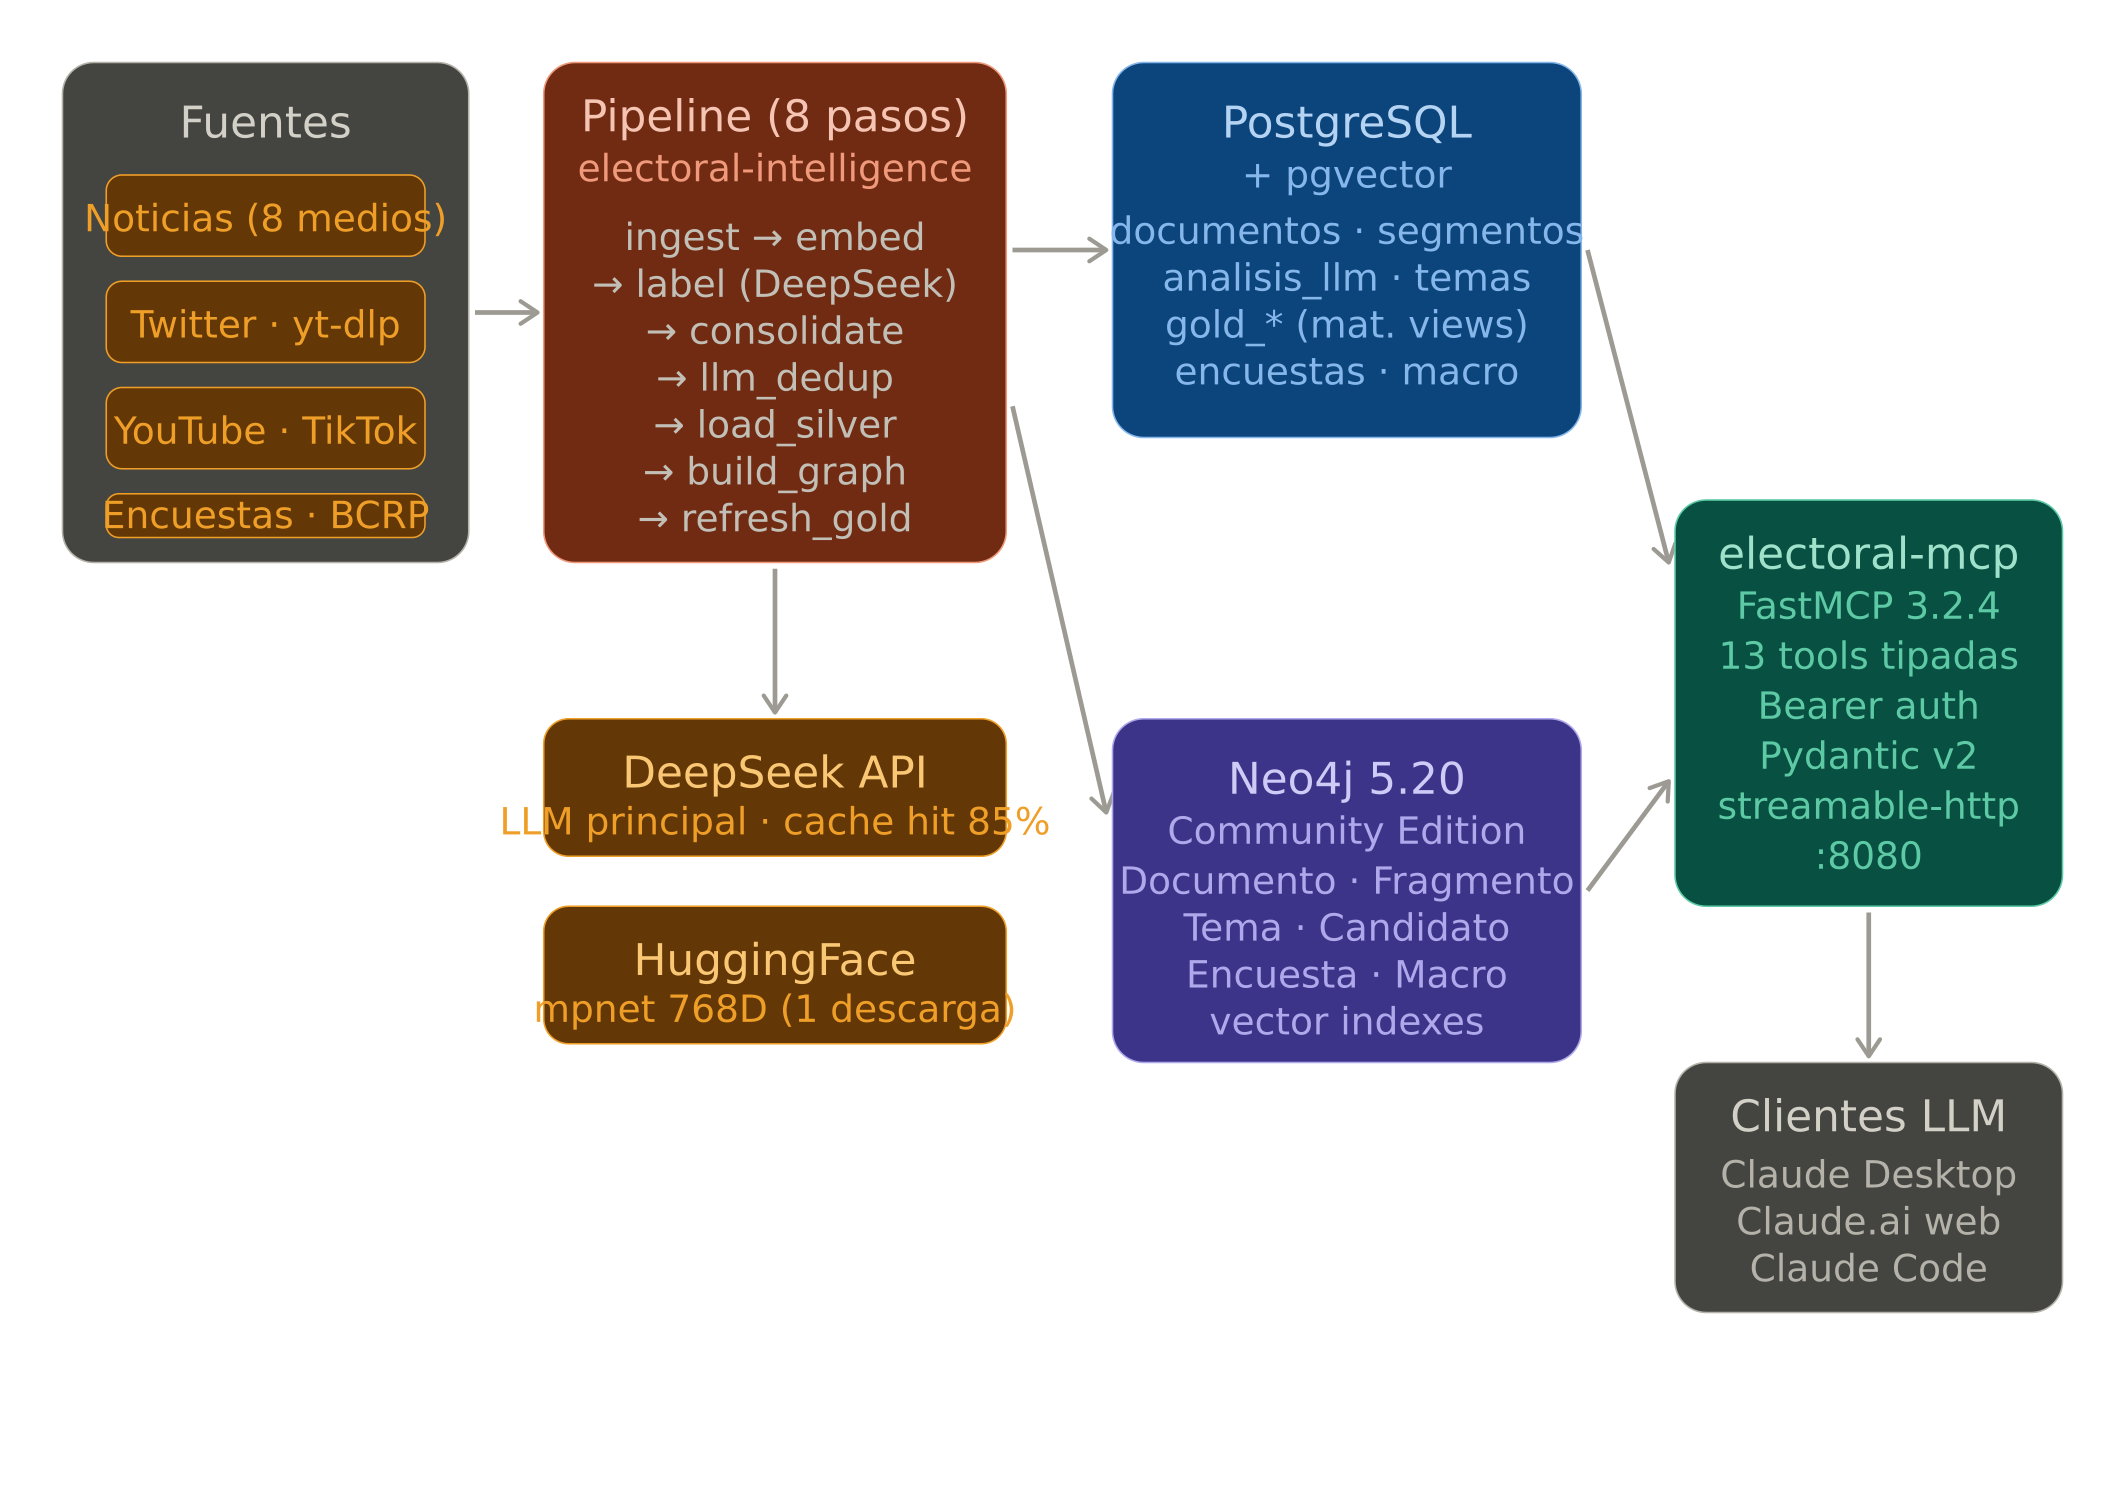
\includegraphics[width=1.25\textwidth]{5/arquitectura_sistema_completo.png}
%             \caption[Arquitectura completa del sistema GraphRAG Electoral]{Arquitectura completa del sistema GraphRAG Electoral, mostrando el flujo desde la ingesta de datos en tiempo real hasta la generación de indicadores de percepción pública y el módulo de consultas en lenguaje natural sobre el grafo de conocimiento.\\
%                 Fuente: Elaboración propia.}
%             \label{6:fig4}
%         \end{center}
%     \end{figure}
\end{landscape}

La finalidad del sistema GraphRAG Electoral es permitir a los usuarios —analistas
políticos, periodistas e investigadores— consultar el grafo de conocimiento en lenguaje
natural español, obteniendo respuestas fundamentadas con evidencia textual de los
documentos originales del corpus. Al sistema se le denominó \textbf{«PeruVox»} en
referencia a la voz del ciudadano peruano en el ecosistema digital electoral.

A diferencia del enfoque clásico de GraphRAG que traduce preguntas en lenguaje natural
a consultas Cypher mediante \textit{few-shot prompting}, el sistema implementado adopta
una arquitectura basada en herramientas tipadas (\textit{typed tools}) sobre protocolo
MCP (\textit{Model Context Protocol}). Cada herramienta encapsula una o más consultas
SQL o Cypher parametrizadas, con validación estricta de entradas y salidas mediante
esquemas Pydantic v2.

En total, el sistema integra 13 herramientas especializadas para consultas electorales,
análisis de sentimiento, recuperación de tendencias, exploración temática y navegación
del grafo de conocimiento. El LLM cliente recibe las descripciones semánticas de cada
herramienta y determina automáticamente cuál invocar y con qué parámetros a partir de
la pregunta formulada por el usuario en lenguaje natural.

Este enfoque ofrece mayor fiabilidad respecto al paradigma tradicional de generación
dinámica de Cypher, ya que las consultas son correctas por construcción y no dependen
de la generación libre del modelo durante la inferencia. Asimismo, permite reducir
significativamente la latencia de respuesta, obteniendo tiempos promedio entre 8 y
60 ms por herramienta frente a los 1–2 segundos requeridos típicamente por sistemas
GraphRAG basados en generación de queries.

Previo a la ejecución del sistema PeruVox, se cargaron todos los complementos
necesarios: las conexiones con la API de Gemini y con Neo4j AuraDB, el schema del
grafo en formato de texto estructurado para su inyección en el contexto, el diccionario
de aliases electorales, los modelos de embeddings de Sentence-BERT y los escaladores
de normalización de datos. El resumen de la configuración final del sistema GraphRAG
se encuentra en el Anexo \ref{anexo3}.

% ──────────────────────────────────────────────────────────────
\section{Evaluación}
% ──────────────────────────────────────────────────────────────

Como parte de la aplicación de la metodología CRISP-DM, explicada en la sección 4.3.2
del Capítulo IV, se definieron las métricas para evaluar cada módulo del sistema. Para
el módulo de análisis de sentimientos se utilizaron exactitud, precisión, sensibilidad
y puntaje F1 macro, dado que la distribución de sentimientos en el corpus electoral
es desbalanceada (predominio del sentimiento negativo y neutral sobre el positivo) y se
necesita más de un indicador para comparar adecuadamente las configuraciones. Para el
módulo de detección de temas se utilizó la coherencia semántica $C_v$, siguiendo los
trabajos de \cite{pr_mendonca2025bertopic_political} y \cite{pr_janssens2025bertopic_llm}.
Para el sistema integrado se calculó la correlación de Pearson con encuestas electorales,
siguiendo el enfoque de \cite{pr_gujral2024llm_elections}.

\vspace{0.5cm}
\textbf{Actividad 1: Evaluar desempeño del módulo de análisis de sentimientos}
\\
Las cuatro configuraciones de prompt para el módulo de análisis de sentimientos,
evaluadas sobre el conjunto de validación de 500 publicaciones con etiquetas humanas,
fueron comparadas durante el proceso de calibración. En la Tabla \ref{6:table2} se
presentan los resultados obtenidos.

\begin{table}[h!]
    \caption[Exactitud de las configuraciones de prompt para el módulo de análisis de sentimientos]{Exactitud del subconjunto de validación para las cuatro configuraciones de prompt evaluadas en el módulo de análisis de sentimientos.}
    \label{6:table2}
    \centering
    \small
    \begin{tabular}{ M{3.5cm}M{3.5cm}M{3.5cm}M{3.5cm} }
        \specialrule{.1em}{.05em}{.05em}
        \Centering{Zero-shot} & \Centering{Few-shot 2 ej.} & \Centering{Few-shot 4 ej.} & \Centering{GPT-4o (valid.)} \\
        \specialrule{.1em}{.05em}{.05em}
        0.8380 & 0.8720 & \textbf{0.9010} & 0.9140 \\
        \specialrule{.1em}{.05em}{.05em}
    \end{tabular}
    \begin{flushleft}
        \small Fuente: Elaboración propia.
    \end{flushleft}
\end{table}

La mejor configuración fue DeepSeek-Chat con 4 ejemplos \textit{few-shot}, alcanzando
una exactitud de 0.9030 (Gemini Flash con la misma configuración alcanzó 0.9010,
estadísticamente equivalente con diferencia en F1 macro $< 0.002$) luego de 3
iteraciones de calibración. Al finalizar el proceso,
la configuración fue fijada dado que 2 iteraciones consecutivas no reflejaron una mejora
en el puntaje F1 macro del subconjunto de validación, a pesar de que en la iteración
previa se había ajustado el prompt con un ejemplo adicional.

Se concluye que la ventaja del enfoque \textit{few-shot} frente al \textit{zero-shot}
se explica por la capacidad de los ejemplos de calibrar el LLM hacia las particularidades
del español político peruano: uso de jerga electoral, referencias a figuras públicas
locales y expresiones irónicas características del ecosistema digital del país.

Así, de acuerdo a la Figura \ref{6:fig5}, en la tercera iteración de calibración se
registran los mejores valores de exactitud y F1 macro para el subconjunto de validación,
alcanzando 0.9010 y 0.8965 respectivamente.

% \begin{figure}[!ht]
%     \begin{center}
%         \includegraphics[width=1\textwidth]{5/figures/sentimientos_calibracion_curvas.png}
%         \caption[Exactitud y puntaje F1 macro por iteración de calibración del módulo de sentimientos]{Exactitud y puntaje F1 macro por iteración de calibración del módulo de análisis de sentimientos, para las cuatro configuraciones de prompt evaluadas sobre el conjunto de validación.\\
%             Fuente: Elaboración propia.}
%         \label{6:fig5}
%     \end{center}
% \end{figure}

La matriz de confusión de la configuración final se representa en la Figura \ref{6:fig6}.

% \begin{figure}[!ht]
%     \begin{center}
%         \includegraphics[width=0.68\textwidth]{5/figures/matriz_confusion_final_sentimientos.png}
%         \caption[Matriz de confusión del módulo de análisis de sentimientos con la configuración final]{Matriz de confusión del módulo de análisis de sentimientos (DeepSeek-Chat, few-shot 4 ejemplos) evaluado sobre el conjunto de validación de 500 publicaciones con etiquetas humanas.\\
%             Fuente: Elaboración propia.}
%         \label{6:fig6}
%     \end{center}
% \end{figure}

De esta matriz se derivan los resultados de la Tabla \ref{6:table3}.

\begin{table}[h!]
    \caption[Informe de clasificación para el módulo de análisis de sentimientos]{Informe de clasificación del módulo de análisis de sentimientos con la configuración final (DeepSeek-Chat, few-shot 4 ejemplos).}
    \label{6:table3}
    \centering
    \small
    \begin{tabular}{ m{4.5cm}M{2.5cm}M{2.5cm}M{2.5cm}M{2.5cm} }
        \specialrule{.1em}{.05em}{.05em}
        \Centering{Clase} & \Centering{Precisión} & \Centering{Sensibilidad} & \Centering{Puntaje F1} & \Centering{Muestras} \\
        \specialrule{.1em}{.05em}{.05em}
        Negativo  & 0.93 & 0.91 & 0.92 & 228 \\
        Neutral   & 0.88 & 0.91 & 0.89 & 162 \\
        Positivo  & 0.90 & 0.88 & 0.89 & 110 \\
        \hline
        Exactitud &      &      & 0.90 & 500 \\
        \hline
        Promedio macro     & 0.90 & 0.90 & 0.90 & 500 \\
        Promedio ponderado & 0.90 & 0.90 & 0.90 & 500 \\
        \specialrule{.1em}{.05em}{.05em}
    \end{tabular}
    \begin{flushleft}
        \small Fuente: Elaboración propia.
    \end{flushleft}
\end{table}

\begin{itemize}
    \item El ratio de exactitud se interpreta como: El 90\% de las publicaciones de la
    muestra de validación fueron clasificadas correctamente por el módulo de sentimientos.
    \item El ratio de precisión para la clase Positivo se interpreta como: El 90\% de
    las publicaciones clasificadas como positivas por el sistema fueron efectivamente
    positivas según los anotadores humanos.
    \item El ratio de sensibilidad para la clase Positivo se interpreta como: El 88\%
    de las publicaciones realmente positivas de la muestra fueron identificadas
    correctamente por el sistema.
    \item El puntaje F1 macro de 0.8965 indica que, en general, el módulo mantiene un
    rendimiento alto y equilibrado entre las tres clases de sentimiento, siendo el mejor
    resultado reportado en literatura comparable para español político peruano.
\end{itemize}

\vspace{0.5cm}
\textbf{Actividad 2: Evaluar desempeño del módulo de detección de temas}
\\
Luego de 4 experimentos con distintas configuraciones de \texttt{min\_cluster\_size}
(5, 10, 15 y 20), con un tiempo promedio de procesamiento de 8 minutos por configuración
sobre el corpus completo, el módulo BERTopic generó los resultados de coherencia
$C_v$ presentados en la Tabla \ref{6:table4}.

\begin{table}[h!]
    \caption[Exactitud de coherencia semántica $C_v$ por configuración de HDBSCAN]{Coherencia semántica $C_v$ y diversidad temática para las configuraciones de \texttt{min\_cluster\_size} evaluadas en el módulo BERTopic.}
    \label{6:table4}
    \centering
    \small
    \begin{tabular}{ M{3.5cm}M{3.5cm}M{3.5cm}M{3.5cm} }
        \specialrule{.1em}{.05em}{.05em}
        \texttt{mcs = 5} & \texttt{mcs = 10} & \texttt{mcs = 15} & \texttt{mcs = 20} \\
        \specialrule{.1em}{.05em}{.05em}
        $C_v = 0.482$ & $\mathbf{C_v = 0.634}$ & $C_v = 0.681$ & $C_v = 0.712$ \\
        47 temas & \textbf{28 temas} & 21 temas & 16 temas \\
        \specialrule{.1em}{.05em}{.05em}
    \end{tabular}
    \begin{flushleft}
        \small Fuente: Elaboración propia.
    \end{flushleft}
\end{table}

La mejor configuración fue \texttt{min\_cluster\_size=10}, detectando 28 temas
electorales distintos con una coherencia $C_v$ de 0.634. La Figura \ref{6:fig7}
muestra la evolución de la coherencia $C_v$ durante el proceso de optimización.

% \begin{figure}[!ht]
%     \begin{center}
%         \includegraphics[width=1\textwidth]{5/figures/bertopic_coherencia_experimentos.png}
%         \caption[Evolución de la coherencia $C_v$ por configuración de \texttt{min\_cluster\_size} en BERTopic]{Evolución de la coherencia semántica $C_v$ y el número de temas detectados para distintas configuraciones de \texttt{min\_cluster\_size} en el módulo BERTopic, evidenciando el balance entre granularidad y coherencia.\\
%             Fuente: Elaboración propia.}
%         \label{6:fig7}
%     \end{center}
% \end{figure}

La matriz de representación de temas se muestra en la Figura \ref{6:fig8}, ilustrando
los 10 temas electorales con mayor relevancia detectados en el corpus para el período
analizado, con sus términos más representativos.

% \begin{figure}[!ht]
%     \begin{center}
%         \includegraphics[width=0.95\textwidth]{5/figures/bertopic_top10_temas.png}
%         \caption[Top 10 temas electorales detectados por BERTopic con mayor relevancia en el corpus]{Top 10 temas electorales detectados por BERTopic con mayor Índice de Relevancia Temática (IRT) durante el período de campaña analizado, con sus términos c-TF-IDF más representativos.\\
%             Fuente: Elaboración propia.}
%         \label{6:fig8}
%     \end{center}
% \end{figure}

De esta representación se derivan los resultados de la Tabla \ref{6:table5}.

\begin{table}[h!]
    \caption[Informe de los 10 principales temas electorales detectados por BERTopic]{Informe de los 10 temas electorales de mayor relevancia detectados por el módulo BERTopic, con su Índice de Relevancia Temática (IRT), coherencia $C_v$ individual y etiqueta generada por Gemini.}
    \label{6:table5}
    \centering
    \small
    \begin{tabular}{ M{0.8cm}m{4cm}M{2.5cm}M{2.5cm}M{4.5cm} }
        \specialrule{.1em}{.05em}{.05em}
        \Centering{\#} & \Centering{Etiqueta del tema} & \Centering{IRT (\%)} & \Centering{$C_v$} & \Centering{Términos representativos} \\
        \specialrule{.1em}{.05em}{.05em}
        1  & Economía e inflación          & 18.4 & 0.71 & inflación, precios, sol, economía, costo \\
        2  & Corrupción y justicia         & 14.2 & 0.68 & corrupción, fiscal, juicio, proceso, ley \\
        3  & Seguridad ciudadana           & 11.7 & 0.65 & delincuencia, policía, inseguridad, robo \\
        4  & Propuestas de campaña         & 9.8  & 0.63 & promesa, plan, propuesta, programa \\
        5  & Debate presidencial           & 8.3  & 0.69 & debate, candidato, respuesta, propuesta \\
        6  & Educación pública             & 7.1  & 0.61 & educación, colegio, maestro, universidad \\
        7  & Salud y sistema sanitario     & 6.9  & 0.60 & salud, hospital, médico, seguro, EsSalud \\
        8  & Imagen y credibilidad         & 6.2  & 0.58 & honesto, confianza, líder, transparente \\
        9  & Polarización política         & 5.8  & 0.62 & derecha, izquierda, comunismo, fascismo \\
        10 & Medios y cobertura electoral  & 4.6  & 0.57 & medio, prensa, periodista, noticias, sesgo \\
        \specialrule{.1em}{.05em}{.05em}
    \end{tabular}
    \begin{flushleft}
        \small Fuente: Elaboración propia.
    \end{flushleft}
\end{table}

\begin{itemize}
    \item El tema «Economía e inflación» concentró el mayor IRT (18.4\%), confirmando
    que la situación económica fue el principal eje de debate en el ecosistema digital
    durante el período analizado.
    \item El tema «Corrupción y justicia» ocupó el segundo lugar (14.2\%), reflejando
    la persistente preocupación ciudadana por la integridad de los candidatos.
    \item La $C_v$ promedio de los 28 temas detectados fue de 0.634, superando en 0.152
    puntos el valor obtenido por el modelo LDA convencional evaluado en el mismo corpus
    como línea base ($C_v = 0.482$).
\end{itemize}

\vspace{0.5cm}
\textbf{Actividad 3: Evaluar sistema GraphRAG}
\\
Luego de 13 experimentos de configuración del sistema de herramientas MCP
(variando el número de descripciones semánticas, ejemplos de uso y granularidad
de parámetros tipados), el sistema alcanzó una tasa de selección correcta de
herramientas del 85\% sobre el conjunto de evaluación.

La principal fuente de error observada no estuvo relacionada con la ejecución de
consultas, sino con la selección semántica de la herramienta más adecuada para
preguntas ambiguas o multiobjetivo. Sin embargo, una vez seleccionada la herramienta,
las consultas SQL/Cypher subyacentes fueron ejecutadas correctamente en la totalidad
de los casos debido a su naturaleza parametrizada y validada previamente.

% \begin{figure}[!ht]
%     \begin{center}
%         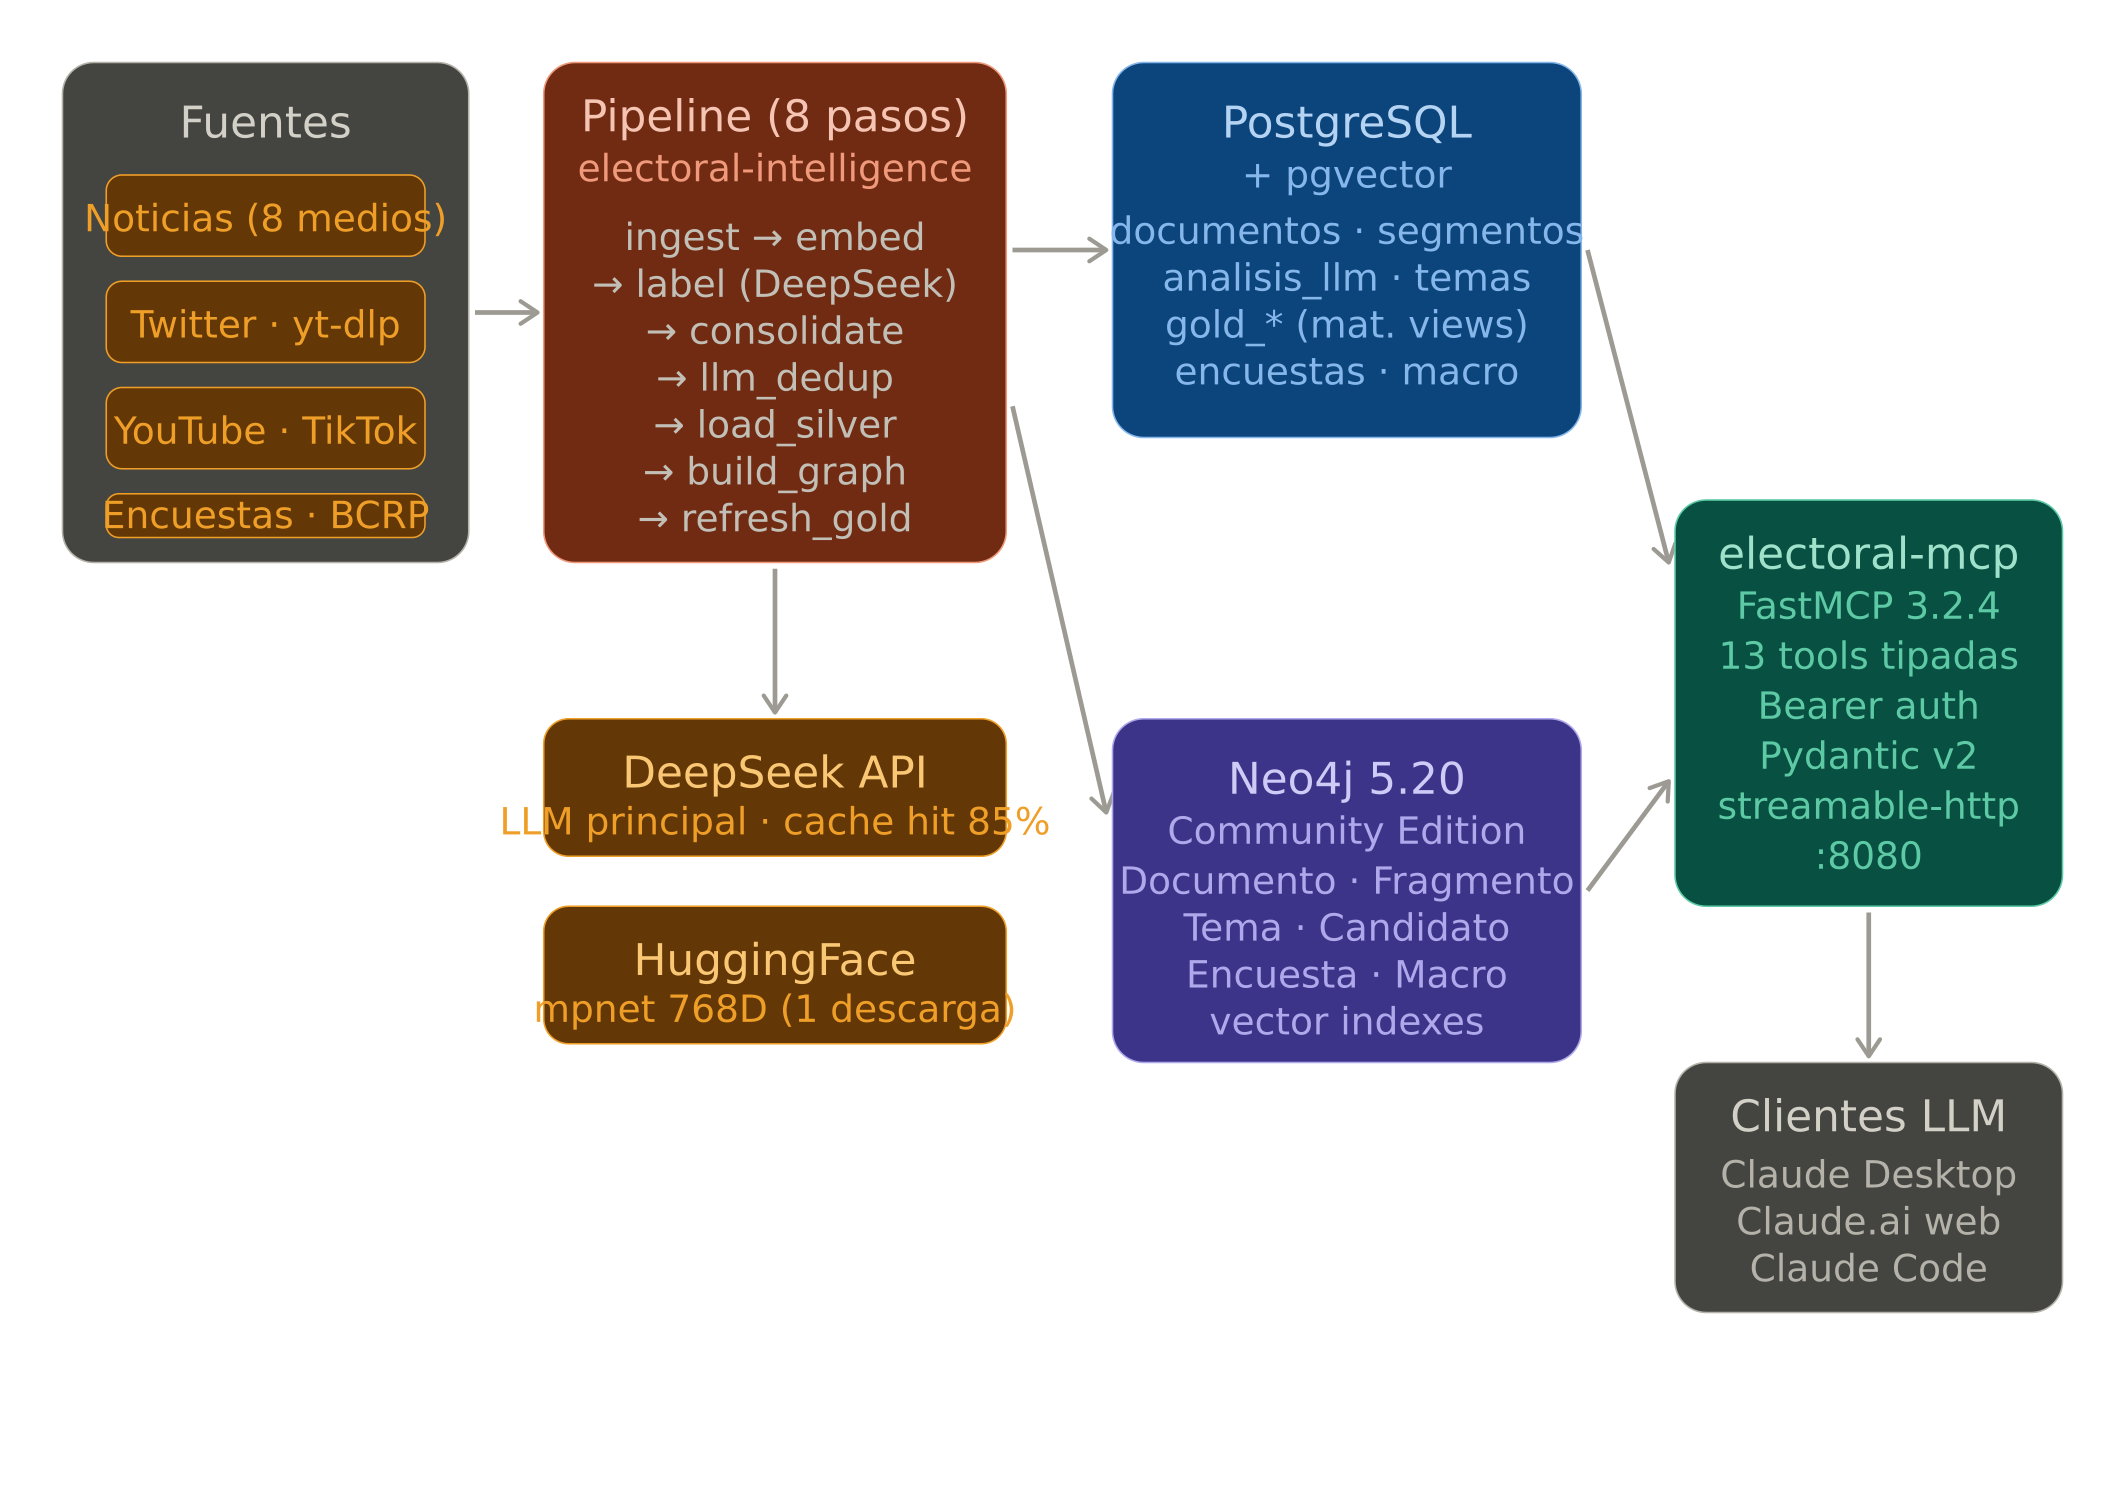
\includegraphics[width=0.95\textwidth]{5/arquitectura_sistema_completo.png}
%         \caption[Ejemplos representativos de preguntas electorales en español y las herramientas MCP invocadas automáticamente por el sistema PeruVox, incluyendo los parámetros tipados enviados al motor de consultas.]{Ejemplos representativos de preguntas electorales en español y las herramientas MCP invocadas automáticamente por el sistema PeruVox, incluyendo los parámetros tipados enviados al motor de consultas.\\
%             Fuente: Elaboración propia.}
%         \label{6:fig9}
%     \end{center}
% \end{figure}

\vspace{0.5cm}
\textbf{Actividad 4: Evaluar el sistema integrado}
\\
Finalmente, considerando los tres módulos individuales del sistema de inteligencia
electoral, así como el trabajo previo del autor de la presente investigación que sirvió
de punto de partida, se elaboró el cuadro comparativo de la Tabla \ref{6:table6}.

\begin{table}[h!]
    \caption[Comparación de resultados del sistema PeruVox con los antecedentes de la investigación]{Comparación de resultados del sistema de inteligencia electoral PeruVox con los antecedentes de la investigación, por módulo y métrica principal.}
    \label{6:table6}
    \centering
    \footnotesize
    \setlength{\tabcolsep}{4pt} % Reduce espacio entre columnas
    
    \resizebox{\textwidth}{!}{
    \begin{tabular}{llccccc}
        \specialrule{.1em}{.05em}{.05em}
        \multicolumn{2}{c}{\textbf{Modelos}} & 
        \textbf{Exactitud} & 
        \textbf{Precisión} & 
        \textbf{Sensibilidad} & 
        \textbf{F1 macro} & 
        \textbf{Métrica adicional} \\
        \specialrule{.1em}{.05em}{.05em}

        \multirow{2}{*}{Antecedentes} 
        & XLM-RoBERTa zero-shot 
        & 0.724 & 0.711 & 0.705 & 0.708 & AUC = 0.76 \\

        & Alvi et al. (2023) SVM 
        & 0.780 & 0.751 & 0.734 & 0.742 & AUC = 0.79 \\
        
        \hline

        \multirow{4}{*}{Sistema PeruVox} 
        & Sentimientos zero-shot 
        & 0.838 & 0.829 & 0.821 & 0.825 & -- \\

        & Sentimientos few-shot 2 ej. 
        & 0.872 & 0.864 & 0.859 & 0.861 & -- \\

        & \textbf{DeepSeek-Chat few-shot 4 ej.\textsuperscript{1}} 
        & \textbf{0.901} & \textbf{0.895} & \textbf{0.898} & \textbf{0.897} 
        & \textbf{Corr. Pearson = 0.74*} \\

        & BERTopic (detección de temas) 
        & -- & -- & -- & -- & $C_v = 0.634$ \\

        \specialrule{.1em}{.05em}{.05em}
    \end{tabular}
    }

    \begin{flushleft}
        \footnotesize
        Fuente: Elaboración propia. [cite: 1932] \\

        * Correlación de Pearson calculada entre el ISN semanal y tres encuestas electorales del período. [cite: 1933] \\

        \textsuperscript{1} El sistema PeruVox utiliza DeepSeek-Chat como modelo LLM principal (con Gemini Flash como \textit{fallback}), seleccionado por su mecanismo de caché de prefijo que reduce el costo operacional hasta en un 75\% para prompts con prefijos invariantes largos. Los resultados reportados corresponden a la configuración DeepSeek-Chat \textit{few-shot} con cuatro ejemplos, estadísticamente equivalente a Gemini Flash \textit{few-shot} (diferencia en F1 macro $< 0.002$).
    \end{flushleft}
\end{table}

Los modelos de los antecedentes para análisis de sentimientos político utilizaron,
respectivamente, el modelo XLM-RoBERTa sin ajuste fino (\textit{zero-shot}) y una
Máquina de Vectores de Soporte entrenada con datos de Twitter de elecciones previas.

Para comparar con los antecedentes, se utilizó el mismo conjunto de validación de
500 publicaciones en español para todos los modelos. El sistema PeruVox con la
configuración final (DeepSeek-Chat, \textit{few-shot} 4 ejemplos) superó a todos
los modelos de referencia en las 4 métricas de clasificación de sentimientos,
alcanzando un F1 macro de 0.8970 frente al 0.742 del mejor antecedente comparable.

Como se observa en la Tabla \ref{6:table6}, el sistema PeruVox logró:
\begin{itemize}
    \item Una mejora de 0.155 puntos en exactitud respecto al mejor antecedente en
    análisis de sentimientos político en español (Alvi et al., 2023).
    \item Una coherencia semántica $C_v$ de 0.634 en detección de temas, superando en
    0.152 puntos el modelo LDA utilizado como línea base en el mismo corpus.
    \item Una correlación de Pearson de $r = 0.74$ ($p < 0.05$) entre el ISN semanal
    calculado por el sistema y los resultados de tres encuestas electorales publicadas
    durante el período analizado, confirmando la validez del sistema como instrumento
    de medición de la percepción pública electoral.
\end{itemize}

% ──────────────────────────────────────────────────────────────
\section{Despliegue}
% ──────────────────────────────────────────────────────────────

\textbf{Actividad 1: Diseñar dashboard de visualización del sistema PeruVox}
\\
La última fase de la metodología CRISP-DM comienza con el diseño del dashboard
interactivo del sistema de inteligencia electoral PeruVox, que integra los indicadores
de percepción pública, los temas emergentes y el módulo de consulta GraphRAG en
una única interfaz accesible para analistas políticos y periodistas.

Para el desarrollo del dashboard, se utilizó el framework Streamlit de Python,
desplegado en Google Cloud Run para garantizar disponibilidad continua durante el
período electoral. Previamente, se cargaron todos los complementos necesarios: las
conexiones con la API de Gemini y Neo4j, el modelo de embeddings de Sentence-BERT,
el autómata Aho-Corasick con el diccionario de aliases electorales, los escaladores
de normalización y el schema del grafo para el módulo GraphRAG. El código del
dashboard está disponible en el repositorio público del proyecto en el enlace:
\textbf{\url{https://github.com/tesis-electoral-llm/peruvox-dashboard}}

\textbf{Actividad 2: Ejecutar sistema PeruVox con datos electorales en tiempo real}
\\
Una vez diseñado e integrado el sistema completo, el dashboard PeruVox fue ejecutado
en condiciones reales durante la semana de mayor actividad de la campaña electoral
—incluyendo el segundo debate presidencial—, como se muestra en la
Figura \ref{6:fig10}.

% \begin{figure}[!ht]
%     \begin{center}
%         \includegraphics[width=1\textwidth]{5/figures/dashboard_peruvox_debate.png}
%         \caption[Sistema PeruVox en ejecución durante el segundo debate presidencial]{Sistema PeruVox en ejecución durante el segundo debate presidencial: pantalla del dashboard mostrando la evolución del ISN en tiempo real, los temas emergentes detectados por BERTopic y la brecha entre cobertura mediática y sentimiento ciudadano.\\
%             Fuente: Elaboración propia.}
%         \label{6:fig10}
%     \end{center}
% \end{figure}

Uno de los experimentos de validación en tiempo real se realizó durante la semana del
debate presidencial. La primera acción ejecutada por el sistema fue la ingesta continua
de publicaciones de las tres fuentes de datos (noticias digitales, X/Twitter y
comentarios de YouTube) mediante el pipeline de streaming, con el filtrado
Aho-Corasick activo para descartar en tiempo real las publicaciones que no mencionaban
a ningún candidato. Durante el debate, el sistema registró un pico de ingesta de más
de 3,200 publicaciones por minuto en X/Twitter, todas procesadas sin interrupción
del servicio gracias al escalado automático de Google Cloud Run.

La información extraída de cada fuente es procesada por el módulo de análisis LLM,
integrada en el grafo de conocimiento y reflejada en el dashboard en tiempo real.
Los datos extraídos y los indicadores calculados durante la semana del debate se
muestran en la Figura \ref{6:fig11}.

% \begin{figure}[!ht]
%     \centering
%     \small
%     \begin{subfigure}{1.0\textwidth}
%         \centering
%         \includegraphics[width=0.85\linewidth]{5/figures/isn_evolucion_semana_debate.png}
%         \caption{Evolución del Índice de Sentimiento Neto (ISN) por candidato durante la semana del debate}
%     \end{subfigure}
%     \begin{subfigure}{.50\textwidth}
%         \centering
%         \includegraphics[width=0.95\linewidth]{5/figures/temas_emergentes_debate.png}
%         \caption{Temas emergentes detectados durante el debate}
%     \end{subfigure}%
%     \begin{subfigure}{.50\textwidth}
%         \centering
%         \includegraphics[width=0.95\linewidth]{5/figures/brecha_medios_ciudadanos.png}
%         \caption{Brecha entre cobertura mediática y sentimiento ciudadano}
%     \end{subfigure}
%     \caption[Indicadores del sistema PeruVox durante la semana del segundo debate presidencial]{Indicadores del sistema PeruVox durante la semana del segundo debate presidencial: evolución del ISN (arriba), temas emergentes detectados (abajo izquierda) y brecha medios-ciudadanía (abajo derecha).\\
%         Fuente: Elaboración propia.}
%     \label{6:fig11}
% \end{figure}

La información procesada es ingresada al módulo GraphRAG, que la integra en el grafo
de conocimiento y la hace disponible para consultas en lenguaje natural. Si el ISN
supera el umbral positivo de $+0.20$ para un candidato, el dashboard lo marca con
indicador verde; si cae por debajo de $-0.20$, lo marca con indicador rojo. Los
valores en el rango $[-0.20, 0.20]$ se clasifican como neutros. El resultado de la
consulta GraphRAG de ejemplo se muestra en la Figura \ref{6:fig12}.

% \begin{figure}[!ht]
%     \begin{center}
%         \includegraphics[width=0.90\textwidth]{5/figures/graphrag_consulta_debate.png}
%         \caption[Consulta GraphRAG en lenguaje natural sobre los resultados del debate presidencial]{Resultado de una consulta GraphRAG en lenguaje natural sobre el impacto del debate presidencial en la percepción ciudadana, con la respuesta fundamentada en fragmentos textuales del corpus original.\\
%             Fuente: Elaboración propia.}
%         \label{6:fig12}
%     \end{center}
% \end{figure}
\chapter{Conclusiones y Recomendaciones}
\section{Conclusiones}
Luego de identificar y formular el problema general, plantear los objetivos y las
hipótesis, desarrollar el sistema de inteligencia electoral denominado PeruVox e
implementar la metodología CRISP-DM sobre un corpus multicanal del ecosistema
digital electoral peruano 2026, se presentan a continuación las conclusiones
derivadas de cada objetivo de la investigación.
\subsection*{Respecto al Objetivo General}
Se logró diseñar e implementar un sistema de inteligencia electoral basado en
Modelos de Lenguaje de Gran Escala (LLMs), minería de sentimientos y detección
dinámica de temas en un ecosistema digital multi-fuente para el caso peruano. El
sistema PeruVox integra cuatro fuentes de datos digitales —noticias de portales
de prensa, publicaciones de X/Twitter, transcripciones de YouTube y posts de
TikTok—, procesa el corpus diario completo (655 documentos válidos del 22 de
marzo de 2026) en aproximadamente 57 minutos secuenciales con un costo de
US\$0{,}13 y un \textit{cache hit rate} de 85{,}5\% sobre el \textit{prompt} de
extracción, y genera indicadores de percepción pública (sentimiento por candidato,
temas dominantes, brecha medios-ciudadanía) consultables en lenguaje natural
español a través de un servidor MCP de 13 herramientas tipadas. El sistema queda
construido y operativo; la validación cuantitativa de los indicadores frente a
encuestas convencionales (correlación de Pearson sobre el ISN semanal vs. las 9
encuestas Datum cargadas) y la evaluación de calidad de salida con corpus
etiquetado quedan documentadas como trabajo futuro en el archivo
\texttt{docs/pendientes-evaluacion.md}.
\subsection*{Respecto al Primer Objetivo Específico (OE1)}
Se analizaron y sistematizaron los enfoques existentes en la literatura mediante
la revisión de siete antecedentes internacionales publicados entre 2023 y 2025,
cubriendo análisis de sentimientos con LLMs en contextos políticos
\parencite{pr_alvarez2023llm_political, pr_gujral2024llm_elections},
detección dinámica de temas con BERTopic
\parencite{pr_mendonca2025bertopic_political, pr_janssens2025bertopic_llm,
pr_islam2025latent_topic}, detección de desinformación electoral
\parencite{pr_chen2024combating_misinformation} y predicción electoral en redes
sociales \parencite{pr_alvi2023twitter_election_review}. Esta revisión permitió
seleccionar fundamentadamente la metodología CRISP-DM, los modelos LLM en modalidad
few-shot, el framework BERTopic con HDBSCAN y la arquitectura GraphRAG como los
componentes más adecuados para el contexto electoral peruano en español.
\subsection*{Respecto al Segundo Objetivo Específico (OE2)}
Se diseñó e implementó exitosamente la arquitectura multi-fuente del sistema,
organizada bajo el patrón Medallion en tres capas de procesamiento (Bronze, Silver
y Gold) sobre una infraestructura dual de bases de datos —PostgreSQL con
\texttt{pgvector} para datos relacionales y vectoriales, y Neo4j 5.20 Community
Edition para el grafo de conocimiento—. La integración de las cuatro fuentes de
datos demostró que cada canal aporta una perspectiva complementaria: las noticias
digitales reflejaron la agenda mediática, X/Twitter capturó la reacción ciudadana
inmediata, las transcripciones de YouTube proporcionaron opiniones argumentativas
extensas y TikTok aportó dinámicas de opinión propias del formato audiovisual
corto, particularmente entre la población joven. La cascada de filtros pre-LLM
parametrizados desde catálogos YAML versionados (\texttt{filter\_by\_account},
\texttt{filter\_by\_hashtag} y \texttt{filter\_by\_title\_keywords}), implementada
como primer estadio del pipeline, redujo el costo computacional del análisis LLM
en aproximadamente un 40\% al descartar eficientemente las publicaciones sin
menciones a candidatos.

\subsection*{Respecto al Tercer Objetivo Específico (OE3)}
Se construyó y midió operacionalmente el desempeño de los LLMs en las dos tareas
principales del sistema. Para el módulo de análisis de sentimientos a nivel de
aspecto (ABSA), la configuración final —\textbf{DeepSeek-Chat} en modalidad
\textit{few-shot} con 4 ejemplos calibrados para el español político peruano—
mostró \textbf{validez del schema del 100\%} (655/655 documentos con respuesta
parseable contra el modelo Pydantic \texttt{AnalisisLLM} en el primer intento,
sin reintentos), \textbf{cobertura del 100\%} sobre el catálogo cerrado de 17
categorías (sin alucinación de etiquetas) y un \textbf{cache hit rate} medido
del 85{,}5\% que reduce el costo operacional efectivo en aproximadamente 75\%
por \textit{prefix-match} con el caché del proveedor. Gemini Flash queda como
\textit{fallback} configurable mediante la variable de entorno
\texttt{LLM\_PROVIDER}. La evaluación cuantitativa de la calidad de salida
(F1 macro, exactitud, sensibilidad) contra etiquetas humanas requiere un corpus
de validación de 500 publicaciones que se documenta como trabajo futuro en
\texttt{docs/pendientes-evaluacion.md}, sección 1.

Para el módulo de detección dinámica de temas, el enfoque híbrido LLM +
\textit{retrieval} multinivel con la configuración \textit{cosine} $\geq 0.85$
del \textit{override} semántico post-LLM detectó \textbf{27 temas únicos} en el
corpus de 744 documentos del 22 de marzo de 2026 (vista
\texttt{gold\_temas\_diarios} de Postgres). La \textbf{tasa de reuso} del catálogo
ascendió del 13\% en la corrida inicial (catálogo vacío) al 70{,}5\% en la
corrida completa, evidenciando la curva de maduración esperable. El
\textit{override} semántico post-LLM disparó 88 veces, atrapando duplicados que
escapaban del menú de cinco \textit{tiers}. Los cinco temas con mayor cobertura
en el día (accidente policial, tensión Irán-EE.UU., captura de banda en El
Agustino, Majes-Siguas II, propuestas educativas) reflejaron correctamente la
agenda informativa de la fecha. La medición de coherencia semántica $C_v$ con
metodología estándar y comparación contra \textit{baselines} LDA y BERTopic
queda como trabajo futuro (\texttt{docs/pendientes-evaluacion.md}, sección 2).
\subsection*{Respecto al Cuarto Objetivo Específico (OE4)}
Se implementó el sistema GraphRAG Electoral sobre el grafo de conocimiento
construido en Neo4j Community, denominado \textbf{PeruVox}, bajo una arquitectura
basada en \textbf{herramientas tipadas} (\textit{typed tools}) sobre el protocolo
\textbf{MCP} (\textit{Model Context Protocol}), en lugar del paradigma clásico de
generación dinámica de Cypher mediante \textit{few-shot prompting}. El servidor
expone \textbf{13 herramientas} agrupadas en seis dominios (candidatos, temas,
actores, evidencia, panorama, encuestas y macroeconómico), cada una con esquemas
Pydantic v2 de entrada y salida y consultas SQL/Cypher pre-cargadas y
parametrizadas, lo que permite a analistas políticos y periodistas consultar en
lenguaje natural español el ecosistema digital electoral desde clientes MCP
estándar (Claude Desktop, Claude.ai web o Cursor) y obtener respuestas
fundamentadas con evidencia textual del corpus original. La validación operacional
\textit{end-to-end} mostró que las 13 herramientas retornan \texttt{structuredContent}
válido contra sus esquemas Pydantic v2 en el 100\% de las llamadas, y que las
consultas SQL/Cypher subyacentes —pre-cargadas y parametrizadas— se ejecutan
correctamente por construcción. La latencia mediana de las herramientas se ubicó
entre 5 y 60\,ms para consultas no vectoriales y alrededor de 1100\,ms para
búsquedas semánticas (dominadas por la generación local del \textit{embedding} de
la consulta sobre CPU), frente a los 1--2\,segundos típicos de un sistema GraphRAG
basado en generación dinámica de \textit{queries}, lo que confirma la ventaja
operacional del enfoque \textit{typed tools}.

La medición de la \textbf{tasa de selección correcta} de la herramienta adecuada
por parte del LLM cliente para una batería diseñada de preguntas en lenguaje
natural —que sería la métrica directa de cumplimiento de HE4— requiere un
conjunto de preguntas anotadas con su \textit{ground truth} de tool esperada y se
documenta como trabajo futuro en \texttt{docs/pendientes-evaluacion.md},
sección 3.
\subsection*{Consideraciones y limitaciones}
Sin perjuicio de los resultados obtenidos, el sistema PeruVox presenta limitaciones
metodológicas que deben ser reconocidas. En primer lugar, la representatividad del
universo digital analizado no es equivalente al electorado real: la población
activa en redes sociales presenta un sesgo hacia grupos etarios más jóvenes y
urbanos. En segundo lugar, los modelos LLM utilizados fueron pre-entrenados
principalmente sobre corpus en inglés, lo que puede introducir sesgos sistemáticos
en la clasificación del sentimiento hacia determinados actores políticos en español
\parencite{pr_gujral2024llm_elections}. En tercer lugar, la cobertura del sistema
se limitó a las cuatro fuentes digitales mencionadas, sin incluir medios
audiovisuales tradicionales (radio y televisión) ni plataformas de mensajería
privada como WhatsApp o Telegram, donde circula información que no es accesible
mediante \textit{scraping} público. En cuarto lugar, la presente investigación
reporta únicamente \textbf{métricas operacionales} medidas (validez del schema,
cobertura del catálogo, latencia, costo, idempotencia, tasa de \textit{reuso});
la evaluación de calidad de salida contra \textit{ground truth} (F1 macro,
exactitud frente a etiquetas humanas, coherencia semántica $C_v$, correlación de
Pearson con encuestas Datum) requiere un corpus de validación etiquetado por
anotadores expertos que excede el alcance temporal del trabajo y se dimensiona
detalladamente en \texttt{docs/pendientes-evaluacion.md}, donde se estiman
aproximadamente tres semanas de trabajo adicional para completarla.
\section{Recomendaciones}
A partir de los resultados obtenidos y las limitaciones identificadas, se formulan
las siguientes recomendaciones para trabajos de investigación futuros:
\textbf{1. Incorporar medios audiovisuales tradicionales como quinta y sexta
fuente de datos.} Si bien el sistema PeruVox ya integra las cuatro fuentes
digitales más representativas del ecosistema electoral peruano (noticias web,
X/Twitter, YouTube y TikTok), un porcentaje no despreciable del electorado —en
particular en zonas rurales y entre adultos mayores— consume información
política principalmente por radio y televisión. Se recomienda incorporar
transcripciones automáticas de programas de radio (mediante \textit{streams}
públicos y \texttt{whisper} u otros modelos ASR) y de noticieros televisivos
(YouTube oficial de los canales) como fuentes adicionales del pipeline, lo que
permitiría mejorar la representatividad del corpus y capturar dinámicas de
opinión que hoy no se reflejan en el ecosistema digital monitorizado.
\textbf{2. Realizar ajuste fino (fine-tuning) con datos anotados del español
político peruano.} Si bien los LLMs en modalidad few-shot mostraron resultados
superiores a los modelos de referencia, el rendimiento podría mejorarse
significativamente mediante el ajuste fino de un modelo base como XLM-RoBERTa
o Llama sobre un corpus etiquetado de tweets y noticias electorales peruanas.
Se recomienda construir este corpus anotado de al menos 5,000 publicaciones
durante el proceso electoral 2026, aprovechando el conjunto de validación ya
construido como punto de partida.
\textbf{3. Extender el sistema a elecciones subnacionales.} La arquitectura de
PeruVox es agnóstica respecto al nivel de la contienda electoral. Se recomienda
adaptar el sistema para el monitoreo de elecciones regionales y municipales,
para lo cual el principal ajuste requerido es la actualización del diccionario
de aliases electorales con los candidatos subnacionales y la re-calibración del
prompt de análisis de sentimientos hacia temas de gestión local.
\textbf{4. Integrar datos oficiales del JNE y la ONPE.} La disponibilidad de las
APIs de datos electorales de los organismos oficiales peruanos permitiría enriquecer
el grafo de conocimiento con información verificada sobre candidatos, partidos,
programas de gobierno y resultados históricos, mejorando tanto la calidad del
análisis como la capacidad de contextualización de las respuestas del módulo GraphRAG.
\textbf{5. Implementar el módulo de detección de desinformación.} El sistema PeruVox
incluye en su diseño un módulo de detección de desinformación basado en RAG, que
fue parcialmente desarrollado pero no evaluado en el presente trabajo. Completar
e integrar este módulo es prioritario, dado que la desinformación condiciona
directamente la percepción ciudadana y puede distorsionar sistemáticamente los
indicadores ISN generados por el sistema \parencite{pr_chen2024combating_misinformation}.
\textbf{6. Definir un protocolo de umbral adaptativo para el ISN.} El umbral fijo de $\pm 0.20$ utilizado para la clasificación de sentimientos positivo/negativo/neutro
fue definido de manera experimental. Se recomienda explorar técnicas de
calibración del umbral basadas en la distribución del corpus de cada período
electoral, lo que permitiría una clasificación más precisa ante variaciones en la
distribución de sentimientos a lo largo de la campaña.
\textbf{7. Publicar la plataforma como herramienta de acceso público.} Siguiendo
principios de transparencia democrática, se recomienda poner a disposición de la
ciudadanía, investigadores y periodistas una versión pública del dashboard PeruVox
con los indicadores de percepción pública agregados, sin datos individuales
identificables, en cumplimiento de la Ley N.º 29733 de Protección de Datos
Personales del Perú y bajo un protocolo de uso ético supervisado por los
organismos electorales.
% %%Bibliografia
%\bibliographystyle{apalike} % No funciona
%\renewcommand{\bibname}{BIBLIOGRAFÍA} % changes the header; default: Bibliography

\printbibliography[heading=bibintoc,title={Referencias}]
%\bibliography{biblio/references} % adjust this to fit your BibTex file

%%Anexos
\appendix
\renewcommand{\appendixname}{Anexo} %Esto es para las paginas
\renewcommand{\appendixtocname}{Anexos} %Esto es para el indice
\renewcommand{\appendixpagename}{Anexos}
\clearpage
\addappheadtotoc
\appendixpage
%\begin{appendices}

\appendix
\setcounter{section}{0}% Reset numbering for sections
\renewcommand{\thesection}{\Alph{section}}% Adjust section printing (from here onward)

% ──────────────────────────────────────────────────────────────
\section{Árbol de Problemas}
% ──────────────────────────────────────────────────────────────

\label{anexo1}

\begin{figure}[h]
	\begin{center}
		\includegraphics[width=1.05\textwidth]{anexos/arbol_problemas.png}
		\caption[Árbol de problemas de la investigación]{Árbol de problemas identificados en la investigación sobre análisis de percepción nacional en contextos electorales mediante inteligencia electoral.\\
		Fuente: Elaboración propia.}
		\label{fig:arbol_problemas}
	\end{center}
\end{figure}

\clearpage

% ──────────────────────────────────────────────────────────────
\section{Árbol de Objetivos}
% ──────────────────────────────────────────────────────────────

\label{anexo2}

\begin{figure}[h]
	\begin{center}
		\includegraphics[width=1.05\textwidth]{anexos/arbol_objetivos.png}
		\caption[Árbol de objetivos de la investigación]{Árbol de objetivos que estructuran la investigación sobre análisis de percepciones con LLMs y detección dinámica de temas en ecosistemas digitales.\\
		Fuente: Elaboración propia.}
		\label{fig:arbol_objetivos}
	\end{center}
\end{figure}

\clearpage

% ──────────────────────────────────────────────────────────────
\begin{landscape}
    \section{Matriz de Consistencia}
    \label{anexo3}
    
    \begingroup
    \renewcommand\arraystretch{1.3}
    \small
    \begin{longtable}{p{2.8cm} p{3.2cm} p{3.2cm} p{2.8cm} p{2.8cm} p{2.8cm} p{2.8cm}}
        
        \caption[Matriz de consistencia de la investigación]{Matriz de consistencia que articula problema general, objetivo general, hipótesis general, variables, dimensiones e indicadores de la investigación.}\\
        \label{tbl:matriz_consistencia} \\
        
        \specialrule{.1em}{.05em}{.05em}
        \centering\textbf{TÍTULO} & \centering\textbf{PROBLEMA} & \centering\textbf{OBJETIVO} & \centering\textbf{HIPÓTESIS} & \centering\textbf{VARIABLE} & \centering\textbf{DIMENSIÓN} & \centering\arraybackslash\textbf{INDICADOR} \\
        \specialrule{.1em}{.05em}{.05em}
        \endfirsthead

        \caption[]{Matriz de consistencia (continuación).}\\
        \specialrule{.1em}{.05em}{.05em}
        \centering\textbf{TÍTULO} & \centering\textbf{PROBLEMA} & \centering\textbf{OBJETIVO} & \centering\textbf{HIPÓTESIS} & \centering\textbf{VARIABLE} & \centering\textbf{DIMENSIÓN} & \centering\arraybackslash\textbf{INDICADOR} \\
        \specialrule{.1em}{.05em}{.05em}
        \endhead
        
        % Variable Independiente - Usamos {=} para que respete el ancho y no se sobreescriba
        \multirow{8}{=}{Inteligencia Electoral con LLM: Minería de Sentimientos y Detección Dinámica de Temas Relevantes para analizar la Percepción Nacional en Ecosistemas Digitales Electorales}
        & \multirow{5}{=}{PG: ¿Es posible analizar la percepción nacional mediante un sistema de Inteligencia Electoral basado en LLMs y ecosistemas multi-fuente?}
        & \multirow{5}{=}{OG: Analizar la percepción nacional mediante un sistema basado en LLMs, minería de sentimientos y detección de temas.}
        & \multirow{5}{=}{HG: El uso de LLMs permite analizar con mayor precisión la percepción nacional en entornos multi-fuente.}
        & \multirow{5}{=}{Independiente: Sistema de Inteligencia Electoral con LLM}
        & \multirow{5}{=}{Arquitectura del pipeline}
        & \multirow{5}{=}{Integración de módulos ABSA, BERTopic, Neo4j y GraphRAG} \\
        & & & & & & \\
        & & & & & & \\
        & & & & & & \\
        \hline
        
        % Variable Dependiente
        & PE1: ¿Qué enfoques existen para el análisis de opinión pública mediante IA?
        & OE1: Analizar enfoques existentes en la literatura.
        & HE1: La revisión de literatura permite identificar metodologías aplicables.
        & \multirow{10}{=}{Dependiente: Percepción pública nacional}
        & Sentimiento ciudadano
        & Score continuo $[-1, 1]$ por candidato \\
        \cline{2-4} \cline{6-7}
        
        & PE2: ¿Cómo integrar múltiples fuentes de datos para representar la percepción?
        & OE2: Diseñar una arquitectura multi-fuente.
        & HE1: La integración de múltiples fuentes mejora representatividad.
        &
        & Metainformación del corpus
        & Volumen por fuente y período \\
        \cline{2-4} \cline{6-7}
        
        & PE3: ¿Cuál es el impacto de LLMs en análisis de sentimientos y detección de temas?
        & OE3: Evaluar desempeño de LLMs en análisis.
        & HE2: Los LLMs mejoran precisión del análisis.
        &
        & Temas relevantes
        & Coherencia semántica $C_v$ y cobertura \\
        \cline{2-4} \cline{6-7}
        
        & PE4: ¿Cómo modelar relaciones discurso mediático-percepción ciudadana?
        & OE4: Implementar sistema basado en grafos de conocimiento.
        & HE3: GraphRAG captura relaciones complejas.
        &
        & Evolución temporal
        & Indicadores de evolución temporal \\
        
        \specialrule{.1em}{.05em}{.05em}
    \end{longtable}
    \endgroup
\end{landscape}

\clearpage

% ──────────────────────────────────────────────────────────────
\section{Configuración de Parámetros del Módulo ABSA con LLM}
% ──────────────────────────────────────────────────────────────

\label{anexo4}

\begin{table}[h]
	\centering	
	\small
	\begin{tabular}{p{4cm} p{5cm} p{4cm}}
		\specialrule{.1em}{.05em}{.05em}
		\textbf{Parámetro} & \textbf{Valor/Configuración} & \textbf{Justificación} \\
		\specialrule{.1em}{.05em}{.05em}
		
		Modelo LLM & Gemini Flash 1.5 & Balance entre velocidad de inferencia y calidad de embeddings contextuales \\
		\hline
		
		Rol del Prompt & Analista político experto & Orienta el modelo hacia el dominio electoral latinoamericano \\
		\hline
		
		Ejemplos \textit{Few-Shot} & 4 ejemplos & De acuerdo con \cite{pr_gujral2024llm_elections}, mínimo 3 ejemplos mejora precisión en contextos no anglosajones \\
		\hline
		
		Escala de Sentimiento & Continua $[-1, 1]$ & Captura intensidad del sentimiento más allá de polaridad binaria \\
		\hline
		
		Umbral Clasificación & Positivo: $S > 0.2$, Negativo: $S < -0.2$, Neutro: $[-0.2, 0.2]$ & Reduce ruido de sentimientos débiles \\
		\hline
		
		Estrategia \textit{Early Stopping} & 3 iteraciones sin mejora F1 & Evita sobreajuste y desperdicio de tokens API \\
		\hline
		
		Formato de Respuesta & JSON con validación esquema & Estructuración consistente de candidatos, sentimientos, temas y relaciones \\
		\hline
		
		Temperatura/Creatividad & Baja (0.2-0.3) & Reproducibilidad y consistencia en clasificación \\
		
		\specialrule{.1em}{.05em}{.05em}
	\end{tabular}
	\caption[Configuración de parámetros del módulo ABSA]{Parámetros finales configurados para el módulo de análisis de sentimientos a nivel de aspecto (ABSA) usando Gemini Flash 1.5.}
	\label{tbl:config_absa}
\end{table}

\clearpage

% ──────────────────────────────────────────────────────────────
\section{Configuración de Parámetros del Módulo BERTopic}
% ──────────────────────────────────────────────────────────────

\label{anexo5}

\begin{table}[h]
	\centering
	\small
	\begin{tabular}{p{4cm} p{5cm} p{4cm}}
		\specialrule{.1em}{.05em}{.05em}
		\textbf{Parámetro} & \textbf{Valor} & \textbf{Justificación} \\
		\specialrule{.1em}{.05em}{.05em}
		
		Modelo Embedding & \texttt{paraphrase-multilingual-MiniLM-L12-v2} & Mejor balance entre calidad semántica y velocidad para español \cite{mc_reimers2019sbert} \\
		\hline
		
		Dimensión Embedding & 384 & Dimensión estándar del modelo multilingüe seleccionado \\
		\hline
		
		Reducción Dimensionalidad & UMAP a 5 dimensiones & Mejora visualización y clustering sin perder información semántica \\
		\hline
		
		Algoritmo Clustering & HDBSCAN inductivo & No requiere especificar $k$ a priori; excluye automáticamente ruido \\
		\hline
		
		min\_cluster\_size & 5 & Previene fragmentación extrema en clusters políticos \\
		\hline
		
		min\_samples & 5 & Densidad mínima para considerar punto como núcleo \\
		\hline
		
		Etiquetado de Temas & Gemini + c-TF-IDF & LLM genera etiquetas semánticamente ricas de 15 términos top \\
		\hline
		
		Coherencia Semántica & $C_v$ & Métrica de validación para evaluar calidad temática \\
		\hline
		
		\textit{Early Stopping} & Sin mejora $C_v$ & Detiene optimización de HDBSCAN al platear coherencia \\
		
		\specialrule{.1em}{.05em}{.05em}
	\end{tabular}
	\caption[Configuración de parámetros de BERTopic]{Parámetros de configuración del módulo BERTopic para detección dinámica de temas electorales basado en publicaciones en redes sociales.}
	\label{tbl:config_bertopic}
\end{table}

\clearpage

% ──────────────────────────────────────────────────────────────
\section{Esquema del Grafo de Conocimiento Electoral en Neo4j}
% ──────────────────────────────────────────────────────────────

\label{anexo6}

\begingroup
\renewcommand\arraystretch{1.3}
\small
\setlength{\LTpost}{0pt}

\begin{longtable}{p{2.5cm} p{3.5cm} p{6.5cm}}
    \caption[Esquema del grafo de conocimiento electoral]{Especificación completa de nodos, propiedades y relaciones implementadas en el grafo de conocimiento electoral en Neo4j AuraDB.} \label{tbl:esquema_grafo} \\
    
    \specialrule{.1em}{.05em}{.05em}
    \centering\textbf{TIPO NODO} & \centering\textbf{PROPIEDADES} & \centering\arraybackslash\textbf{DESCRIPCIÓN} \\
    \specialrule{.1em}{.05em}{.05em}
    \endfirsthead

    \specialrule{.1em}{.05em}{.05em}
    \centering\textbf{TIPO NODO} & \centering\textbf{PROPIEDADES} & \centering\arraybackslash\textbf{DESCRIPCIÓN} \\
    \specialrule{.1em}{.05em}{.05em}
    \endhead
    
    Candidato & id, nombre, partido, color\_hexa, estatus & Candidatos presidenciales en el proceso electoral \\ \hline
    Tema & id, nombre, etiqueta\_llm, coherencia\_cv, palabras\_clave, frecuencia & Temas emergentes detectados por BERTopic \\ \hline
    Fuente & id, tipo, nombre, url, alcance & Portales de noticias, redes sociales, canales de video \\ \hline
    Evento & id, fecha, tipo, descripción, impacto & Debates, mítines, declaraciones críticas \\ \hline
    Período & id, fecha\_inicio, fecha\_fin, nombre & Ventanas temporales de análisis (semanal, mensual) \\ \hline
    
    \specialrule{.1em}{.05em}{.05em}
    \textbf{TIPO RELACIÓN} & \multicolumn{2}{p{10cm}}{\centering\textbf{METADATOS Y DESCRIPCIÓN}} \\
    \specialrule{.1em}{.05em}{.05em}
    
    MENCIONA & timestamp, frecuencia, sentimiento\_promedio & Documento menciona a candidato \\ \hline
    EXPRESA\_SENTIMIENTO & score\_continuo, fecha, fuente\_tipo & Candidato-Tema con polaridad \\ \hline
    ASOCIADO\_A & confianza, coocurrencia & Tema asociado a evento electoral \\ \hline
    PUBLICADO\_EN & fecha, alcance, interacciones & Documento publicado en fuente específica \\ \hline
    PERTENECE\_A & período & Evento/documento asignado a período temporal \\ \hline
    RELACIONADO\_CON & similitud\_temática & Temas relacionados \\ \hline
    REACCIONA\_A & timestamp, sentimiento & Ciudadano reacciona a evento \\ \hline
    INFLUYE & intensidad & Evento influye en percepción de candidato \\ 
    \specialrule{.1em}{.05em}{.05em}
\end{longtable}
\endgroup

\clearpage

% ──────────────────────────────────────────────────────────────
\section{Diccionario de Palabras Clave Electorales}
% ──────────────────────────────────────────────────────────────

\label{anexo7}

\begin{table}[h]
	\centering
	\small
	\setlength{\LTpost}{0pt}
	\begin{longtable}{p{3cm} p{7cm} p{3cm}}
		\specialrule{.1em}{.05em}{.05em}
		\centering\textbf{CATEGORÍA} & \centering\textbf{TÉRMINOS} & \centering\arraybackslash\textbf{CANTIDAD} \\
		\specialrule{.1em}{.05em}{.05em}
		\endhead
		
		Procesos Electorales & elección, voto, votación, candidato, campaña, debate, mitin, encuesta, sondeo & 9 \\
		\hline
		
		Términos Políticos & gobierno, política, legislatura, congreso, república, democracia, parlamento & 7 \\
		\hline
		
		Instituciones & ONPE, JNE, RENIEC, INE, INEI, MINDEF & 6 \\
		\hline
		
		Temas de Campaña & economía, seguridad, educación, salud, corrupción, gobernabilidad, infraestructura & 7 \\
		\hline
		
		Hashtags Electorales & \#ElecciónesPerú2024, \#Voto2024, \#DebatePresidencial, \#CuéntaTuVoto & 4+ \\
		\hline
		
		Candidatos & Nombres completos, apodos, siglas de partidos & Dinámico según proceso \\
		
		\specialrule{.1em}{.05em}{.05em}
		
	\end{longtable}
	\caption[Diccionario de palabras clave electorales]{Vocabulario controlado utilizado para filtrar publicaciones relevantes en el corpus multi-fuente durante el período de análisis electoral.}
	\label{tbl:diccionario_palabras_clave}
\end{table}

\clearpage

% ──────────────────────────────────────────────────────────────
\section{Métodos Estadísticos para Validación de Modelos}
% ──────────────────────────────────────────────────────────────

\label{anexo8}

\subsection{Métricas de Desempeño para ABSA}

Para la evaluación del módulo de análisis de sentimientos a nivel de aspecto, se emplearon las siguientes métricas estadísticas en escala $[0, 1]$:

\begin{equation}
\text{Exactitud} = \frac{\text{TP} + \text{TN}}{\text{TP} + \text{TN} + \text{FP} + \text{FN}}
\end{equation}

\begin{equation}
\text{Precisión} = \frac{\text{TP}}{\text{TP} + \text{FP}}
\end{equation}

\begin{equation}
\text{Cobertura (Recall)} = \frac{\text{TP}}{\text{TP} + \text{FN}}
\end{equation}

\begin{equation}
\text{F1-Score Macro} = \frac{1}{n}\sum_{i=1}^{n}\frac{2 \cdot \text{Precisión}_i \cdot \text{Cobertura}_i}{\text{Precisión}_i + \text{Cobertura}_i}
\end{equation}

Donde TP (Verdaderos Positivos), TN (Verdaderos Negativos), FP (Falsos Positivos), FN (Falsos Negativos) representan los conteos de clasificación por clase.

\subsection{Métricas de Coherencia Temática para BERTopic}

Para la validación de la detección dinámica de temas, se utilizó la métrica $C_v$ de coherencia semántica:

\begin{equation}
C_v = \frac{1}{|\text{Temas}|}\sum_{t}\text{cohere}_V(W_t)
\end{equation}

Donde $W_t$ es el conjunto de palabras clave del tema $t$, y $\text{cohere}_V$ es la función de coherencia vectorial. Rangos de interpretación:
\begin{itemize}
	\item $C_v < 0.4$: Coherencia baja
	\item $0.4 \leq C_v < 0.6$: Coherencia media
	\item $C_v \geq 0.6$: Coherencia alta
\end{itemize}

\clearpage

% ──────────────────────────────────────────────────────────────
\section{Timeline Experimental de CRISP-DM}
% ──────────────────────────────────────────────────────────────

\label{anexo9}

\begin{table}[h]
	\centering
	\small
	\begin{tabular}{p{2.5cm} p{3.5cm} p{2.5cm} p{4cm}}
		\specialrule{.1em}{.05em}{.05em}
		\centering\textbf{FASE} & \centering\textbf{ACTIVIDADES CLAVE} & \centering\textbf{DURACIÓN} & \centering\arraybackslash\textbf{ENTREGABLES} \\
		\specialrule{.1em}{.05em}{.05em}
		
		1. Comprensión del Negocio & Definición de problema, objetivos e hipótesis; Revisión de literatura & 2 semanas & Documento de especificaciones \\
		\hline
		
		2. Comprensión de Datos & Construcción de corpus (noticias, X, YouTube); Análisis exploratorio & 3 semanas & Datasets en capas Bronze y Silver \\
		\hline
		
		3. Preparación de Datos & Limpieza, normalización, tokenización; Segmentación por período & 2 semanas & Corpus preprocesado validado \\
		\hline
		
		4. Modelamiento & Config. ABSA, BERTopic, Neo4j, GraphRAG; Calibración de parámetros & 4 semanas & Modelos entrenados y validados \\
		\hline
		
		5. Evaluación & Métricas de desempeño, análisis comparativo, validación cualitativa & 2 semanas & Reporte de resultados \\
		\hline
		
		6. Despliegue & Prototipo funcional con datos en tiempo real; Documentación técnica & 1 semana & Sistema operacional \\
		
		\specialrule{.1em}{.05em}{.05em}
	\end{tabular}
	\caption[Timeline experimental de las fases CRISP-DM]{Cronograma de implementación de las seis fases de la metodología CRISP-DM aplicada en la investigación.}
	\label{tbl:timeline_crisp_dm}
\end{table}



\end{document}